%-*- coding=utf-8 -*-

% 声明文档的类型是ctexart(即ctex-article, 用于写中文TEX的文章),\ 默认行间距为1.25倍,\ 并且要求双面打印
\documentclass[UTF8, twoside]{ctexart}

% A4纸,\ 上边距为2.5cm,\ 下边距为2.0cm,\ 左边距为2.5cm,\ 右边距为2.0cm
\usepackage{geometry}
\geometry{a4paper, top=2.5cm, bottom=2.0cm, left=2.5cm, right=2.0cm}

% 使用graphicx宏包,\ 方便插入外部图片
\usepackage{graphicx}

% 用graphicx宏包定义合适的点乘符号·
\makeatletter
\newcommand*\bigcdot{\mathpalette\bigcdot@{.5}}
\newcommand*\bigcdot@[2]{\mathbin{\vcenter{\hbox{\scalebox{#2}{$\m@th#1\bullet$}}}}}
\makeatother

% 使用titlesec宏包,\ 方便改变各级标题的大小
\usepackage{titlesec}

% 一级标题:\ 三号黑体
% 二级标题:\ 小三号黑体
% 三级标题:\ 四号黑体
\titleformat*{\section}{\centering \heiti \bfseries \zihao{3}}
\titleformat*{\subsection}{\centering \heiti \bfseries \zihao{-3}}
\titleformat*{\subsubsection}{\centering \heiti \bfseries \zihao{4}}

% 使用tocloft宏包,\ 方便修改目录格式
% 可参考https://www.zhihu.com/question/41960738/answer/176773198
\usepackage{tocloft}
\renewcommand\cftdot{…}  % 更改目录引导点为中文省略号
\renewcommand{\cftdotsep}{0}  % 更改引导线中两点的间距为0(无间距)
\renewcommand{\cftsecleader}{\cftdotfill{\cftdotsep}}  % 中文文档默认无引导点,\ 因此为一级标题section补上引导点
\renewcommand{\cftsubsecleader}{\cftdotfill{\cftdotsep}}  % 为二级标题subsection补上引导点
\renewcommand{\cftsubsubsecleader}{\cftdotfill{\cftdotsep}}  % 为三级标题subsubsection补上引导点
\renewcommand{\cfttoctitlefont}{\heiti \zihao{3}}  % 设置目录题头为三号黑体,\ 目录居中放在\begin{center}环境中即可

% 使用fancyhdr宏包,\ 方便调整页面格式
\usepackage{fancyhdr}
\pagestyle{fancy}
\fancyhf{}  % 清除所有的页眉页脚
\fancyhead[EC]{Witt向量简介}  % 偶数页页眉 论文题目 居中
\fancyhead[OC]{汕头大学本科毕业论文(设计)}  % 奇数页页眉 xx大学本科毕业论文(设计) 居中
\cfoot{\thepage}  % 页脚 页码 居中

% 声明文献格式
\bibliographystyle{plain}

% 引入cite宏包使得正文参考文献的引用命令有效
\usepackage{cite}

% 引入ntheorem宏包,\ 给证明末尾自动加证毕符号
\usepackage[thmmarks]{ntheorem}
{  % 利用分组,\ 令格式设置效果只作用于证明环境
	\theoremstyle{nonumberplain}
	\theoremheaderfont{\bfseries}
	\theoremsymbol{\mbox{$\Box$}}
	\newtheorem{proof}{\heiti 证明}  % 注意证明末尾要空一个空格出来,\ 不然方框不显示
}
{  % 利用分组,\ 令格式设置效果只作用于证明环境
	\theoremstyle{nonumberplain}
	\theoremheaderfont{\bfseries}
	\newtheorem{zhuji}{\heiti 注记}  % 注意证明末尾要空一个空格出来,\ 不然方框不显示
}

% 设置定理类环境格式
\theoremstyle{plain}

% 定义定理类环境  (放在引入ntheorem宏包后面)
\newtheorem{dingyi}{定义}[subsection]
\newtheorem{yinli}[dingyi]{引理}
\newtheorem{dingli}[dingyi]{定理}
\newtheorem{tuilun}[dingyi]{推论}
\newtheorem{mingti}[dingyi]{命题}
\newtheorem{lizi}[dingyi]{例子}
\newtheorem{suanfa}[dingyi]{算法}
\newtheorem{xingzhi}[dingyi]{性质}

\newtheorem{dingyi4}{定义}[subsubsection]
\newtheorem{yinli4}[dingyi4]{引理}
\newtheorem{dingli4}[dingyi4]{定理}
\newtheorem{tuilun4}[dingyi4]{推论}
\newtheorem{mingti4}[dingyi4]{命题}
\newtheorem{lizi4}[dingyi4]{例子}
\newtheorem{xingzhi4}[dingyi4]{性质}
\newtheorem{suanfa4}[dingyi4]{算法}

% 添加amssymb宏包,\ 增加可用的数学字体(如\mathbb)
\usepackage{amssymb}

% 引入宏包并准备索引
\usepackage{makeidx}  % 调用makeidx宏包,\ 开启索引列表排版功能
\makeindex  % 开启索引功能

% 引入其他宏包
\usepackage{amsmath}  % 分式\dfrac, \tfrac, \begin{gather}环境
\usepackage{mathtools}  % 使用方括号
\usepackage[all,pdf]{xy} % 使用交换图表语言
\usepackage{bm}
\usepackage{extarrows}

% 设置目录,\ 参考文献跳转(一定要放最后)
\usepackage{hyperref} 
\hypersetup{hidelinks}  % 隐藏掉碍眼的跳转提示框

% 导言区与正文分割线--------------------------------------------------------------------------------

% 正文部分
\begin{document}
	
	% 进入封面
	
	% 此页不设置页码
	\thispagestyle{empty}
	
	% 插入汕大校徽图
	
\includegraphics[height=2cm, width=6.35cm]{汕大校徽.jpg}
	
	\vskip 2cm
	
	% 鉴定书标题
	\begin{center}
		\kaishu \zihao{-0} 本科毕业论文(设计)
	\end{center}
	
	\vskip 3cm
	
	% 题目
	\kaishu \zihao{2}
	\quad 题\quad 目:\underline{\qquad \ Witt向量简介 \qquad \ }
	
	\vskip 3cm

	% 学院,\ 系别,\ 专业年级,\ 学生姓名,\ 学号,\ 指导老师
	\kaishu \zihao{3}
	\qquad \ 学\qquad 院:\underline{\qquad \qquad \qquad 理学院 \qquad \qquad \qquad }
	\vskip 0.2cm
	\qquad \ 系\qquad 别:\underline{\qquad \qquad \qquad 数学系 \qquad \qquad \qquad }
	\vskip 0.2cm
	\qquad \ 专业年级:\underline{\qquad \ 2017级数学与应用数学 \qquad \ \ }
	\vskip 0.2cm
	\qquad \ 学生姓名:\underline{\qquad \qquad \qquad 吴\quad 彬 \qquad \qquad \qquad }
	\vskip 0.2cm
	\qquad \ 学\qquad 号:\underline{\qquad \qquad \quad \ 2017061033 \qquad \qquad \quad \ }
	\vskip 0.3cm
	\qquad \ 指导教师:\underline{\qquad \qquad \qquad 陈\quad 哲 \qquad \qquad \qquad }
	
	\vskip 4cm
	
	% 完成时间
	\begin{center}
		完成时间:2021年5月
	\end{center}
	
	% 封面到此结束
	\newpage
	% 此页不设置页码
	\thispagestyle{empty}
	\ 
	\newpage
	
	% 进入诚信承诺书
	
	% 此页不设置页码
	\thispagestyle{empty}
	
	% 承诺书标题
	\begin{center}
		\zihao{-2} \heiti
		汕头大学本科生毕业论文(设计)诚信承诺书
	\end{center}
	
	\vskip 1cm
	
	% 承诺内容
	\kaishu \zihao{-3}
	本人承诺呈交的毕业论文(设计)《Witt向量简介》是在指导教师的指导下,独立开展研究取得的成果,
	文中引用他人的观点和材料,
	均在文后按顺序列出其参考文献,
	论文(设计)使用的数据真实可靠。
	
	\vskip 1.5cm
	
	% 签名与日期
	{
	\kaishu \zihao{-3}
	\qquad \qquad \qquad \qquad \qquad \qquad \qquad 
	本人签名:\underline{\qquad \quad \ 吴\quad 彬 \qquad \quad \ }
	
	\vskip 0.3cm
	
	\qquad \qquad \qquad \qquad \qquad \qquad \qquad 
	日\qquad 期:\underline{\qquad \ 2021年5月\  \qquad }
	}

	% 承诺书到此结束
	\newpage
	% 此页不设置页码
	\thispagestyle{empty}
	\ 
	\newpage
	
	% 进入中文摘要页
	
	% 摘要和目录设置罗马字体页码
	\pagenumbering{roman}
	
	% 中文题目
	\begin{center}
		\heiti \zihao{2}
		\textbf{Witt向量简介}
	\end{center}
	
	% 摘要题头
	\begin{center}
		\heiti \zihao{-2}
		\vskip 0.4cm
		摘要
	\end{center}
	
	% 中文摘要内容
	\zihao{-4}
	本文研究了整数环$\mathbb{Z}$关于赋值结构的完备化结果在环同构意义下的另一种代数表示. 我们先介绍环上的赋值概念, 然后引入赋值等价这个二元关系, 并在Ostrowski定理的帮助下将$\mathbb{Z}$上赋值的研究范围缩小到三种典型结构. 在指出$\mathbb{Z}$只关于其中的$p$-进赋值不完备之后, 我们对其完备化得到一个精简的结果: ${{\mathbb{Z}}_{p}}$. 之后我们研究了其剩余域${{\mathbb{F}}_{p}}$上的一种特殊环结构: Witt环$\mathcal{W}\left( {{\mathbb{F}}_{p}} \right)$, 并借助Teichmüller提升${{\tau }_{e}}$实现了$\mathcal{W}\left( {{\mathbb{F}}_{p}} \right)$与${{\mathbb{Z}}_{p}}$的环同构.
	\vskip 0.2cm
	\noindent {\heiti 关键词: Witt向量 \qquad Teichmüller提升 \qquad  Ostrowski定理 \qquad p-进赋值}
	\vskip 1.5cm
	
	% 进入英文摘要页
	
	% 英文题目
	\begin{center}
		\zihao{2}
		\textbf{An introduction to Witt vectors}
	\end{center}

	% 摘要题头
	\begin{center}
		\zihao{-2}
		\vskip 0.4cm
		\textbf{Abstract}
	\end{center}
	
	% 英文摘要内容
	\zihao{-4}
	This paper studies an isomorphic representation of the completion of integer ring $\mathbb{Z}$ under the structure of valuation. First we introduce the concept of valuation and equivalence between valuations as a binary relation. With the help of Ostrowski Theorem we narrow down the range of valuations on $\mathbb{Z}$ to three classic types. Then we point out that $\mathbb{Z}$ only is not completed under p-adic valuation, after which we complete it and have a simple result: ${{\mathbb{Z}}_{p}}$. Then on its residue field ${{\mathbb{F}}_{p}}$ we study a special ring: Witt ring $\mathcal{W}\left( {{\mathbb{F}}_{p}} \right)$. Finally we successfully use Teichmüller lift ${{\tau }_{e}}$ to build isomorphism between $\mathcal{W}\left( {{\mathbb{F}}_{p}} \right)$ and ${{\mathbb{Z}}_{p}}$.
	\vskip 0.2cm
	\noindent {\bfseries Key Words: Witt vectors\qquad Teichmüller lift \qquad Ostrowski Theorem \qquad p-adic valuation}
	
	% 英文摘要页到此结束
	\newpage
	\ 
	\newpage
	
	% 进入目录页
	\begin{center}
		\tableofcontents
	\end{center}
	\newpage
	\ 
	\newpage
	
	\section*{前言}
	\addcontentsline{toc}{section}{前言}  % 将该节以不编号的形式加入到目录
	\zihao{-4}
	在进入正文前, 首先声明该文除去一些关键的思路和证明, 也存在一部分
	{\heiti 完全由本人给出的证明过程或例子}, 涉及但不限于以下内容: 
	\begin{description}
		\item[\S~1.1] 命题1.1.2, 推论1.1.7, 命题1.1.9.
		
		\item[\S~1.2] 命题1.2.4, 命题1.2.5, 命题1.2.6, 命题1.2.7, 命题1.2.8, 命题1.2.9, 
		引理1.2.10, 引理1.2.11, 推论1.2.14.
		
		\item[\S~1.3] 例子1.3.2, 例子1.3.3, 命题1.3.5, 例子1.3.6, 例子1.3.7, 例子1.3.8,
		例子1.3.9, 命题1.3.11, 命题1.3.12, 命题1.3.13, 定理1.3.15.
		
		\item [\S~2.1] 命题2.1.1, 推论2.1.2, 定理2.1.3.
		
		\item [\S~2.2] 命题2.2.1, 命题2.2.3, 命题2.2.5, 命题2.2.10, 推论2.2.11, 
		例子2.2.13, 例子2.2.14.
		
		\item[\S~3.1] 命题3.1.4, 命题3.1.8, 命题3.1.11
		
		\item[\S~3.2] 命题3.2.1, 命题3.2.2, \S~3.2.1中除去引理3.2.1.11的剩余部分, 
		引理3.2.2.6, 推论3.2.2.7, \S~3.2.3全部的证明过程.
		
		\item[\S~3.3] 命题3.3.1.3, 定理3.3.1.4.
	\end{description}
	
	注意虽然上面的内容的证明或例子完全由本人提供, 但是这些命题, 定理, 例子的提出也有部分是来源于或者启发于文后
	所录的一些参考文献. 包括关键思路和定理的提供和证明, 每一小节的最核心的参考文献如下.
	\begin{description}
		\item[\S~1] Neukirch\cite{neukirch}, Enochs\cite{enochs}.
		
		\item[\S~2] 李文威\cite{liwenwei}.
		
		\item[\S~3] 李文威\cite{liwenwei}, Witt\cite{Witt}, Serre\cite{serre}.
	\end{description}
	文中具体涉及到引用的地方也会再次特别标注出来.
	
%	% 进入常用记号部分-----------------------------------------------------------------------------------------
%	\section*{常用记号}
%	\addcontentsline{toc}{section}{常用记号}  % 将该节以不编号的形式加入到目录
%	\zihao{-4}
%	\begin{itemize}
%		\item $\mathbb{Q}$:\ 有理数集.\ 
%		\item 
%	\end{itemize}
	% 进入正文-------------------------------------------------------------------------------------------------
	
	% 正文显示阿拉伯数字的页码
	\pagenumbering{arabic}
	
%	% 进入正文引言一节------------------------------------------------------------------------------------------
%	\section{引言}
%	\zihao{-4}
	
	
	% 进入完备化一节------------------------------------------------------------------------------------------
	\newpage
	\ 
	\newpage
	\section{整数环${\mathbb{Z}}$的完备化}
	\numberwithin{equation}{subsection}  % 规定公式编号格式(加上小节的编号前缀)
	\zihao{-4}
	基于柯西列收敛意义的“完备化”一词在不同的学科有着不同的定义.\ 
	具体到我们研究的整数集$\mathbb{Z}$,\ 
	若将其视为一个带有度量\cite[第二章\S~1]{chengqixiang}的集合,\ 则其完备化是在“度量”意义下的,\ 
	完备化的结果是完备度量空间\cite[第七章\S~4]{chengqixiang};\ 
	若将其视为一个带有范数\cite[第六章\S~3]{xiadaoxing}的线性空间结构,\ 则其完备化是在“范数”意义下的,\ 
	完备化的结果是完备赋范线性空间\cite[第六章\S~5]{xiadaoxing}.\ 
	而本文我们将整数集$\mathbb{Z}$视为一个环结构,\ 所讨论的“完备化”是在“赋值”意义下的.\ 
	以下第1小节我们先介绍关于赋值的一些数学基础,\ 
	然后在第2小节聚焦于$\mathbb{Z}$的分式域$\mathbb{Q}$上的赋值,\ 在等价意义下对所关注的赋值种类的范围进行收缩,\ 
	最后在第3小节简单讨论一下$\mathbb{Z}$的完备化问题.\ 
	\\ \phantom{哈哈}
	
	\subsection{环上赋值基础} % 2.1------------------------------------------------------------------------------
	\zihao{-4}
	我们先引入与完备化相关的一个核心概念:\ 赋值.\ 
	\begin{dingyi} \label{赋值定义}
		设$\Re$是一个环.\ 称单射$\left| \bigcdot \right|: \ \Re \mapsto \mathbb{R}_{\ge 0}$是$\Re$
		上的一个{\heiti 赋值}\index{赋值},\ 若$\left| \bigcdot \right|$满足
		\begin{enumerate}
			\item $\left| x \right| = 0.\ \Longleftrightarrow\ x = \bm{0};$
			\item $\left| xy \right| = \left| x \right| \left| y \right|,\ \forall x,\ y \in \Re;$
			\item $\left| x + y \right| \le \left| x \right| + \left| y \right|,\ \forall x,\ y \in \Re.$
		\end{enumerate}
	\end{dingyi}
	\vskip 0.5cm
	
	基于上面的定义,\ 环上赋值有如下几个基本的性质.\ 
	\begin{mingti} \label{赋值性质}
		环$\Re$上的赋值$\left| \bigcdot \right|$满足以下的性质(1),\ (2),\ (3).\ 特别地,\ 若$\Re =\mathbb{K}$是一个域,\ 则额外满足性质(4).\ 
		\begin{enumerate}
			\item $\left| \bm{1} \right| = 1;$
			\item $\left| -\bm{1} \right| = 1;$
			\item $\left| -x \right| = \left| x \right|,
			\ \forall x \in \Re;$
			\item $\left| \dfrac{x}{y} \right| = \dfrac{\left| x \right|}{\left| y \right|},
			\ \forall x\in \mathbb{K},\ \forall y\in {{\mathbb{K}}_{\ne \bm{0}}}.$
		\end{enumerate}
	\end{mingti}
	\begin{proof}
		\phantom{哈哈}
		\begin{enumerate}
			\item 由定义\ref{赋值定义}条件(2),\ 成立
			\begin{equation} \label{1.2.1}
				\left| r \right| \times \left| \bm{1} \right| = 
				\left| r \times \bm{1} \right| = \left| r \right|,\ \forall r \in \Re.
			\end{equation}
			规定$r \ne \bm{0}$,\ 由定义\ref{赋值定义}条件(1),\ 成立
			\begin{equation} \label{1.2.2}
				\left| r \right| \ne 0.
			\end{equation}
			在式(\ref{1.2.2})的基础上,\ 将式(\ref{1.2.1})两边同时除以$\left| r \right|$,\ 即可得到$\left| \bm{1} \right| = 1$.
			\vskip 0.3cm
			
			\item 由定义\ref{赋值性质}条件(2),\ 对于$-\bm{1} \in \Re$,\ 成立
			\begin{equation*}
				\left| \bm{1} \right| = \left| \left( -\bm{1} \right) \times \left( -\bm{1} \right) \right| = 
				\left| -\bm{1} \right| \times \left| -\bm{1} \right|,
			\end{equation*}
			即有$\left| -\bm{1} \right|^2 = 1$. 由于$\left| -\bm{1} \right| \ge 0$,\ 因此只能是$\left| -\bm{1} \right| = 1$.
			\vskip 0.3cm
			
			\item 由定义\ref{赋值定义}条件(2),\ 成立
			\begin{equation*}
				\left| -r \right| = \left| \left( -\bm{1} \right) r \right| = 
				\left| -\bm{1} \right| \left| r \right| = \left| r \right|,\ \forall r \in \Re.
			\end{equation*}
			\vskip 0.3cm
			
			\item $\forall x \in \mathbb{K}$,\ $\forall y \in \mathbb{K}_{\ne \bm{0}}$,\ 有$x/y \in \mathbb{K}$,\ 且$\left| y \right|\ne 0$. 
			由定义\ref{赋值定义}条件(2),\ 成立
			\begin{equation*}
				\left| x \right| = 
				\left| \frac{x}{y} y \right| = 
				\left| \frac{x}{y} \right| \left| y \right|.\ 
				\Longrightarrow
				\ \left| \frac{x}{y} \right| = 
				\frac{\left| x \right|}{\left| y \right|}. 
			\end{equation*}
		\end{enumerate}
	\vskip 0.3cm
	至此,\ 明所欲证.\ 
	\end{proof}
	\vskip 0.5cm
	
	我们想要对环上的众多赋值进行梳理.\ 
	借由以下定义,\ 我们从一个角度对含幺环上的赋值进行二分类.\ 
	\begin{dingyi} \label{赋值阿基米德性}
		设$\Re$是一个含幺环,\ $\left| \bigcdot \right|$是$\Re$上的一个赋值.\ 记
		\[
			\bm{n} := \underbracket{\bm{1}+\bm{1}+\cdots+\bm{1}}_{n\text{个}},\ \forall n\in {{\mathbb{Z}}_{>0}},
		\]
		其中$\bm{1}$是$\Re$的幺元.\ 
		\begin{enumerate}
			\item 称$\left| \bigcdot \right|$具有{\heiti 非阿基米德性},\ 若$\exists M \in \mathbb{R}_{\ge 0}$,\ 使得
			$\forall n \in \mathbb{Z}_{>0}$,\ $\left| \bm{n} \right| \le M;$
			
			\item 否则称$\left| \bigcdot \right|$具有{\heiti 阿基米德性}\index{阿基米德性},\ 
			即$\forall M \in \mathbb{R}_{\ge 0}$,\ 
			$\exists n \in \mathbb{Z}$,\ 使得$\left| \bm{n} \right| > M$. 
		\end{enumerate}
	\end{dingyi}
	\vskip 0.5cm
	
	在这样的分类视角下,\ 参考J. Neukirch\cite[Proposition 3.6]{neukirch},\ 我们指出非阿基米德赋值存在以下一个很好的等价数学表示.\ 
	\begin{mingti} \label{强三角不等式}
		设$\Re$是一个含幺环,\ 
		$\left| \bigcdot \right|$是$\Re$上的一个非阿基米德赋值,\ 
		当且仅当$\left| \bigcdot \right|$满足{\heiti 强三角不等式}\index{强三角不等式}
		\begin{equation*}
			\left| \bm{x} + \bm{y} \right| \le \max\{\left| \bm{x} \right|,\ \left| \bm{y} \right|\},\ \forall x,\ y \in \mathbb{Z}.
		\end{equation*}
	\end{mingti}
	\begin{proof}
		\phantom{哈哈}
		\begin{enumerate}
			\item 先证明$\Leftarrow$方向的推理是成立的.\ \\
			已知成立
			\begin{equation} \label{1.6.1}
				\left| \bm{x} + \bm{y} \right| \le \max\{\left| \bm{x} \right|,\ \left| \bm{y} \right|\},\ \forall x,\ y \in \mathbb{Z}.
			\end{equation}
			\vskip 0.3cm
			\begin{enumerate}
				\item 第一步,\ 我们指出成立
				\begin{equation} \label{1.6.2}
				\begin{gathered}
					\left| \bm{x_1} + \bm{x_2} + \dots + \bm{x_n} \right| \le 
					\max\{\left| \bm{x_1} \right|,\ \left| \bm{x_2} \right|,\ \dots,\ \left| \bm{x_n} \right|\},\\
					\forall n \in \mathbb{Z}_{>0},\ \forall x_1,\ x_2,\ \dots,\ x_n \in \mathbb{Z}. 
				\end{gathered}
				\end{equation}
				当$n=1$时,\ 显然有$\left| \bm{x_1} \right| = \max\{\left| \bm{x_1} \right|\}.$\\
				假设$n=k$时成立
				\begin{equation} \label{202102171958}
					\left| \bm{x_1} + \bm{x_2} + \dots + \bm{x_k} \right| \le 
					\max\{\left| \bm{x_1} \right|,\ \left| \bm{x_2} \right|,\ \dots,\ \left| \bm{x_k} \right|\}.
				\end{equation} 
				由式(\ref{1.6.1})和式(\ref{202102171958}),\ 有
				\begin{align*}
					& \left| \bm{x_1} + \bm{x_2} + \dots + \bm{x_k} + \bm{x_{k+1}} \right|. \\
					= & \left| \left( \bm{x_1} + \bm{x_2} + \dots + \bm{x_k} \right) + \bm{x_{k+1}} \right|. \\
					\le & \max\{\max\{\left| \bm{x_1} \right|,\ \left| \bm{x_2} \right|,\ \dots,\ \left| \bm{x_k} \right|\},\ 
					\left| \bm{x_{k+1}} \right|\}. \\ 
					= & \max\{\left| \bm{x_1} \right|,\ \left| \bm{x_2} \right|,\ \dots,\ 
					\left| \bm{x_k} \right|,\ \left| \bm{x_{k+1}} \right|\}.
				\end{align*}
				由第一数学归纳法\cite[\S~1.3.3]{quwanlin},\ 式(\ref{1.6.2})成立.\ 
				\vskip 0.3cm
				
				\item 第二步,\ 我们指出成立
				\[
					\left| \bm{n} \right| \le 1,
					\ \forall n \in \mathbb{Z}_{>0}.
				\]
				事实上,\ $\forall n \in \mathbb{Z}_{>0}$,\ 由第一步的结论有
				\begin{equation*}
					\left| \bm{n} \right| = \left| \underbracket{\bm{1}+\dots+\bm{1}}_{n\text{个}} \right| \le 
					\max\{\left| \bm{1} \right|,\ \dots,\ \left| \bm{1} \right|\} = 1.
				\end{equation*}
				由定义\ref{赋值阿基米德性},\ $\left| \bigcdot \right|$具有非阿基米德性.\ 
			\end{enumerate}
			\vskip 0.3cm
			
			\item 再证明$\Rightarrow$方向的推理是成立的.\ \\
			此方向下,\ 已知$\left| \bigcdot \right|$具有非阿基米德性.\ 
			\vskip 0.3cm
			\begin{enumerate}
				\item 第一步,\ 我们指出成立
				\begin{equation}\label{1.6.3}
				\begin{gathered}
					\left| \bm{x} + \bm{y} \right| \le M^{\frac{1}{n}} \left( 1 + n \right) ^ {\frac{1}{n}} 
					\max\{\left| \bm{x} \right|,\ \left| \bm{y} \right|\}, \\
					\forall n \in \mathbb{Z}_{>0},
					\ \forall x,\ y \in \mathbb{Z},
					\ \exists M \in \mathbb{R}_{\ge 0}.
				\end{gathered}
				\end{equation}
				事实上,\ 由于$\left| \bigcdot \right|$具有非阿基米德性,\ 根据定义\ref{赋值阿基米德性},\ 成立
				\begin{equation} \label{202102191510}
					\left| \bm{n} \right| \le M,
					\ \exists M \in \mathbb{R}_{\ge 0},
					\ \forall n \in \mathbb{Z}_{>0}.
				\end{equation}
				由于$\forall v \in \{ 1,\ \dots,\ n \}$,\ 
				组合数$\binom{n}{v} \in \mathbb{Z}_{>0}$\footnote{组合数是正整数的严格证明详见附录\ref{贾宪数}.\ }
				\cite[第一章 \S~5]{minsihe},\ 由式(\ref{202102191510}),自然也就成立
				\begin{equation} \label{1.6.4}
					\left| \binom{n}{v} \right| \le M.
				\end{equation}
				$\forall x,\ y \in \mathbb{Z}$,\ 不妨令$\left| \bm{x} \right| \ge \left| \bm{y} \right| \ge 0$,\ 成立
				\begin{equation} \label{1.6.5}
					\left| \bm{x} \right|^v \left| \bm{y} \right| ^{n-v} \le
					\left| \bm{x} \right|^v \left| \bm{x} \right| ^{n-v} = 
					\left| \bm{x} \right| ^n,
					\ \forall v \in \{1,\ \dots,\ n\}.
				\end{equation}
				考虑$\left| \bm{x}+\bm{y} \right|^n$,\ 由定义\ref{赋值定义}条件(2),\ 有
				\begin{equation} \label{1.6.6}
					\left| \bm{x}+\bm{y} \right|^n = 
					\underbracket{\left| \bm{x}+\bm{y} \right| \dots \left| \bm{x}+\bm{y} \right|}_{n\text{个}} = 
					\left| \left( \bm{x}+\bm{y} \right)^n \right|.
				\end{equation}
				由定义\ref{赋值定义}条件(2),\ 条件(3), 式(\ref{1.6.4}),\ 式(\ref{1.6.5}),\ 成立
				\begin{align*}
					\left| \left( \bm{x}+\bm{y} \right) ^n \right|
					=& \left| \sum_{v=0}^{n} \binom{n}{v} \bm{x}^v \bm{y}^{n-v} \right|.\\
					\le& \sum_{v=0}^{n} \left| \binom{n}{v}  \bm{x} ^v  \bm{y}^{n-v} \right|. \\
					=& \sum_{v=0}^{n} \left| \binom{n}{v} \right| \left| \bm{x} \right|^v \left| \bm{y} \right|^{n-v}. \\
					\le&  \sum_{v=0}^{n} M \left| \bm{x} \right|^n
					= M\left( n+1 \right) \left| \bm{x} \right| ^n,
				\end{align*} 
				即得到
				\begin{equation} \label{1.6.7}
					\left| \left( \bm{x}+\bm{y} \right)^n \right| \le M \left( n+1 \right) \left| \bm{x} \right| ^n.
				\end{equation}
				由式(\ref{1.6.6})和式(\ref{1.6.7})即可得到
				\begin{equation} \label{1.6.8}
					\left| \bm{x} + \bm{y} \right|^n \le
					M \left( n+1 \right) \left| \bm{x} \right|^n = 
					M \left( n+1 \right) \left( \max\{\left| \bm{x} \right|,\ \left| \bm{y} \right|\} \right) ^n.
				\end{equation}
				式(\ref{1.6.8})两边同时开$n$次方,\ 即可得式(\ref{1.6.3})成立.\ 
				\vskip 0.3cm
				
				\item 第二步,\ 我们分别计算$\lim_{n \rightarrow \infty} M^{{1}/{n}}$和
				$\lim_{n \rightarrow \infty} \left( 1+n \right)^{{1}/{n}}$. \\ 
				对于$M^{{1}/{n}}$,\ 显然有$\lim_{n \rightarrow \infty}M^{{1}/{n}} = 1$. \\
				对于$\left( 1+n \right) ^ {{1}/{n}}$,\ 先考虑其对数
				$\ln \left( 1+n \right) ^ {{1}/{n}} = \frac{\ln \left( 1+n \right)}{n}$.
				由洛必达法则\cite[第六章 \S~2]{shuxuefenxi1},\ 有
				\begin{equation*}
					\lim_{n \rightarrow \infty} \frac{\ln \left( 1+n \right)}{n} = 
					\lim_{n \rightarrow \infty} \frac{1}{1+n} = 0.
				\end{equation*}
				于是有
				\begin{equation*}
					\lim_{n \rightarrow \infty} \left( 1+n \right) ^ {\frac{1}{n}} = 
					\lim_{n \rightarrow \infty} \mathtt{e} ^ {\frac{1}{n} \ln \left( 1+n \right)} = 
					\mathtt{e} ^ {\lim_{n \rightarrow \infty} \frac{1}{n} \ln \left( 1+n \right)} = 
					\mathtt{e}^0 = 1.
				\end{equation*}
				\vskip 0.3cm
				
				\item 第三步,\ 我们指出成立
				\begin{equation} \label{202102191821}
					\left| \bm{x}+\bm{y} \right| \le \max\{\left| \bm{x} \right|,\ \left| \bm{y} \right|\}.
				\end{equation}
				事实上,\ 基于第二步,\ 令式(\ref{1.6.3})两边的$n \rightarrow \infty$,\ 即有
				\begin{equation*}
					\left| \bm{x}+\bm{y} \right| \le M^{\frac{1}{n}} \left( 1+n \right)^{\frac{1}{n}} 
					\max\{\left| \bm{x} \right|,\ \left| \bm{y} \right|\} \rightarrow
					\max\{\left| \bm{x} \right|,\ \left| \bm{y} \right|\}\ \left( n \rightarrow \infty \right).
				\end{equation*}
			由极限的保不等式性\cite[定理2.5]{shuxuefenxi1},\ 式(\ref{202102191821})成立.
			\end{enumerate}
		\end{enumerate}
		\vskip 0.3cm
		至此,\ 明所欲证.\ 
	\end{proof}
	
	\begin{tuilun}  \label{强三角不等式推论}
		设$\Re$是一个含幺环,\ 
		$\left| \bigcdot  \right|$是$\Re$上的一个非阿基米德赋值.\ 
		$\forall {{x}_{1}}$,\ ${{x}_{2}}$,\ $\cdots$,\ ${{x}_{n}}\in \mathbb{Z}\ \left(1 \le n<\infty  \right)$,\ 成立
		\[
			\left| \bm{{x}_{1}}+\bm{{x}_{2}}+\cdots +\bm{{x}_{n}} \right|\le \max \left\{ \left| \bm{{x}_{i}} \right|:\ 
			i=1,\ 2,\ \cdots,\ n \right\}.
		\]
	\end{tuilun}
	\begin{proof}
		$n=1$时结论是显然的.\ $n=2$时结论已由命题\ref{强三角不等式}给出.\ 
		假设$n=k$时成立
		\begin{equation} \label{202102191530}
			\left| \bm{{x}_{1}}+\bm{{x}_{2}}+\cdots +\bm{{x}_{k}} \right|\le \underset{1\le i\le k}{\mathop{\max }}\,\left\{ \left| \bm{{x}_{i}} \right| \right\}.
		\end{equation}
		由于$\left| \bigcdot  \right|$是非阿基米德的, 根据命题\ref{强三角不等式}和式(\ref{202102191530}),\ 有
		\begin{align*}
			&\left| \bm{{x}_{1}}+\bm{{x}_{2}}+\cdots +\bm{{x}_{k}}+\bm{{x}_{k+1}} \right|. \\
			=&\left| \left( \bm{{x}_{1}}+\bm{{x}_{2}}+\cdots +\bm{{x}_{k}} \right)+\bm{{x}_{k+1}} \right|. \\ 
			 \le& \max \left\{ \left| \bm{{x}_{1}}+\bm{{x}_{2}}+\cdots +\bm{{x}_{k}} \right|,\ \left| \bm{{x}_{k+1}} \right| \right\}. \\ 
			 \le& \max \left\{ \underset{1\le i\le k}{\mathop{\max }}\,\left\{ \left| \bm{{x}_{i}} \right| \right\},\ \left| \bm{{x}_{k+1}} \right| \right\}. \\
			 =&\underset{1\le i\le k+1}{\mathop{\max }}\,\left\{ \left| \bm{{x}_{i}} \right| \right\}.
		\end{align*}
		由第一数学归纳法,\ 推论得证.\ 
	\end{proof}
	\vskip 0.5cm
	
	更进一步地,\ 我们可以得到关于含幺环上非阿基米德赋值的一个很好的性质.\ 
	\begin{mingti} \label{强三角不等式推论2}
		设$\Re$是一个含幺环,\ 
		$\left| \bigcdot \right|$是$\Re$上的一个赋值.\ 
		若$\left| \bigcdot \right|$具有非阿基米德性,\ 则$\forall x,\ y \in \mathbb{Z}$,\ 
		当$\left| \bm{x} \right| \ne \left| \bm{y} \right|$时成立{\heiti 严格三角等式}\index{严格三角等式}
		\[
			\left| \bm{x}+\bm{y} \right| = \max\{\left| \bm{x} \right|,\ \left| \bm{y} \right|\}.
		\]
	\end{mingti}
	\begin{proof}
		由于$\left| \bm{x} \right| \ne \left| \bm{y} \right|$,\ 不失一般性地规定$\left| \bm{x} \right| > \left| \bm{y} \right|$. 
		$\left| \bigcdot \right|$是非阿基米德的,\ 由命题\ref{强三角不等式},\ $\forall x,\ y \in \mathbb{Z}$,\ 成立
		\begin{equation} \label{1.7.1}
			\left| \bm{x}+\bm{y} \right| \le \max\{\left| \bm{x} \right|,\ \left| \bm{y} \right|\}.
		\end{equation}
		在上式中令$\bm{x}:=\bm{x}+\bm{y} \in \Re$,\ $\bm{y}:=-\bm{y} \in \Re$,\ 得到
		\begin{equation} \label{1.7.2}
			\left| \bm{x} \right| = \left| \left( \bm{x}+\bm{y} \right) - \bm{y} \right| \le 
			\max\{\left| \bm{x}+\bm{y} \right|,\ \left| -\bm{y} \right|\} = 
			\max\{\left| \bm{x}+\bm{y} \right|,\ \left| \bm{y} \right| \}.
		\end{equation}
		由式(\ref{1.7.1}),\ 式(\ref{1.7.2}),\ 成立
		\begin{equation} \label{202102191535}
			\left| \bm{x} \right| \le \max\{\left| \bm{x}+\bm{y} \right|,\ \left| \bm{y} \right|\} 
			\le \max\{\left| \bm{x} \right|,\ \left| \bm{y} \right| \} = \left| \bm{x} \right|.
		\end{equation}
		基于式(\ref{202102191535}), 成立以下推理
		\[
			\left. \begin{matrix}
				\max \left\{ \left| \bm{x}+\bm{y} \right|,\ \left| \bm{y} \right| \right\}=\left| \bm{x} \right|.  \\
				\left| \bm{x} \right|>\left| \bm{y} \right|. 
			\end{matrix} \right\}\ \Longrightarrow \ \left| \bm{x}+\bm{y} \right|=\left| \bm{x} \right|=\max \left\{ \left| \bm{x} \right|,\ \left| \bm{y} \right| \right\}.
		\]
		至此,\ 明所欲证.\ 
	\end{proof}
	\begin{tuilun} \label{强三角不等式推论3}
		设$\Re $是一个含幺环,\ $\left| \bigcdot  \right|$是$\Re $上的一个非阿基米德赋值.\ $\forall n\in {{\mathbb{Z}}_{\ge 2}}$,\ $\forall {{x}_{1}}$,\ ${{x}_{2}}$,\ $\cdots$,\ ${{x}_{n}}\in \mathbb{Z}$,\ 若它们的赋值两两不等,\ 即$\forall i\ne j\in \left\{ 1,\ 2,\ \cdots ,\ n \right\}$,\ $\left| \bm{{x}_{i}} \right|\ne \left| \bm{{x}_{j}} \right|$,\ 则成立
		\[
		\left| \sum\limits_{k=1}^{n}\bm{{{x}_{k}}} \right|=\underset{1\le k\le n}{\mathop{\max }}\,\left\{ \left| \bm{{x}_{k}} \right| \right\}.	
		\]
	\end{tuilun}
	\begin{proof}
		\ 
		\begin{enumerate}
			\item 第一步,\ 我们指出$\forall n\in {{\mathbb{Z}}_{\ge 2}}$,\ 在成立条件
			\begin{equation} \label{202102191553}
				\forall {{x}_{1}},\ {{x}_{2}},\ \cdots,\  {{x}_{n}}\in \mathbb{Z},\ \textup{s.t.}
				\left| {{x}_{i}} \right|\ne \left| {{x}_{j}} \right|,\ \forall i\ne j,
			\end{equation}
			的前提下,\ 成立
			\begin{equation} \label{202102190114}
					\left| \sum\limits_{\begin{smallmatrix} 
							1\le k\le n \\ 
							k\ne {{k}_{0}} 
					\end{smallmatrix}}^{{}}\bm{{{x}_{k}}} \right|\ne \left| \bm{{x}_{{{k}_{0}}}} \right|,\ 
				\forall {{k}_{0}}\in \left\{ 1,\ 2,\ \cdots ,\ n \right\},
			\end{equation}
			并记$X:=\left\{ {{x}_{1}},\ {{x}_{2}},\  \cdots ,\ {{x}_{n}}\in \mathbb{Z} \right\}$.\\
			任意挑选$2$个满足条件(\ref{202102191553})的${{x}_{i,1}},\ {{x}_{i,2}}\in X$,\ 显然有$\left| \bm{{x}_{i,1}} \right|\ne \left| \bm{{x}_{i,2}} \right|$. \\
			假设任意挑选满足条件(\ref{202102191553})的$j\left( <n \right)$个${{x}_{i,1}},\ {{x}_{i,2}},\ \cdots ,\ {{x}_{i,j}}\in X$,\ 均成立
			\begin{equation} \label{202102191545}
				\left| \sum\limits_{\begin{smallmatrix} 
						1\le k\le j \\ 
						k\ne {{k}_{0}} 
				\end{smallmatrix}}^{{}}\bm{{{x}_{i,k}}} \right|\ne \left| \bm{{x}_{i,{{k}_{0}}}} \right|,
			\ \forall {{k}_{0}}\in \left\{ 1,\ 2,\ \cdots ,\ j \right\}.
			\end{equation}
			则任意挑选$j+1$个满足条件(\ref{202102191553})的${{x}_{i,1}},\ {{x}_{i,2}},\ \cdots ,\ {{x}_{i,j}},\ {{x}_{i,j+1}}\in X$,\ $\forall {{k}_{0}}\in \left\{ 1,\ 2,\ \cdots ,\ j+1 \right\}$,\ 再任取${{k}_{1}}\in \left\{ 1,\ 2,\ \cdots ,\ j+1 \right\}$满足${{k}_{1}}\ne {{k}_{0}}$,\ 由式(\ref{202102191545}),\ 命题\ref{强三角不等式推论2},\ 条件(\ref{202102191553}),\ 成立
			\[
				\left| \sum\limits_{\begin{smallmatrix} 
						1\le k\le j+1 \\ 
						k\ne {{k}_{0}} 
				\end{smallmatrix}}^{{}}\bm{{{x}_{i,k}}} \right|=\left|\left( \sum\limits_{\begin{smallmatrix} 
						1\le k\le j+1 \\ 
						k\ne {{k}_{0}},{{k}_{1}} 
				\end{smallmatrix}}^{{}}\bm{{{x}_{i,k}}}
			\right)
			+\bm{{x}_{i,{{k}_{1}}}} \right|=\max \left\{ \left| \sum\limits_{\begin{smallmatrix} 
						1\le k\le j+1 \\ 
						k\ne {{k}_{0}},{{k}_{1}} 
				\end{smallmatrix}}^{{}}\bm{{{x}_{i,k}}} \right|,\left| \bm{{x}_{i,{{k}_{1}}}} \right| \right\}\ne \left| \bm{{x}_{i,{{k}_{0}}}} \right|.
			\]
			由第一数学归纳法,\ 式(\ref{202102190114})成立.\ 
			\vskip 0.3cm
			
			\item 第二步,\ 基于第一步的结论,\ 并根据命题\ref{强三角不等式推论2},\ 成立
			\begin{align*}
				\left| \sum\limits_{k=1}^{n}\bm{{{x}_{k}}} \right|&=\left| \left( \sum\limits_{k=1}^{n-1}\bm{{{x}_{k}}}
				\right)
				+\bm{{x}_{n}} \right|. \\ 
				& =\max \left\{ \left| \sum\limits_{k=1}^{n-1}\bm{{{x}_{k}}} \right|,\left| \bm{{x}_{n}} \right| \right\}. \\ 
				& =\max \left\{ \max \left\{ \left| \sum\limits_{k=1}^{n-2}\bm{{{x}_{k}}} \right|,\left| \bm{{x}_{n-1}} \right| \right\},\left| \bm{{x}_{n}} \right| \right\}=\max \left\{ \left| \sum\limits_{k=1}^{n-2}\bm{{{x}_{k}}} \right|,\left| \bm{{x}_{n-1}} \right|,\left| \bm{{x}_{n}} \right| \right\}. \\ 
				& =\cdots.  \\ 
				& =\underset{1\le k\le n}{\mathop{\max }}\,\left\{ \left| \bm{{x}_{k}} \right| \right\}.
			\end{align*}
		\end{enumerate}
	\vskip 0.3cm
	至此,\ 明所欲证.\ 
	\end{proof}
	\vskip 0.5cm
	
	对含幺环上众多赋值进行分类和性质探讨后,\ 我们想引入“等价”概念对这些赋值建立起联系,\ 以实现进一步的梳理.\ 
	等价概念的建立需要借助拓扑学基础,\ 于是我们参考尤承业\cite[第一章 \S~1]{youchengye},\ 先引入相关的基本概念.\ 
	\begin{dingyi} \label{度量定义}
		设$X$是一个集合,\ 称$X$上的一个映射$d:\ X \times X \mapsto \mathbb{R}_{\ge 0}$是一个{\heiti 度量}\index{度量},\ 
		若$d$满足:\ 
		\begin{enumerate}
			\item $d \left( x,y \right) = 0.\ \Longleftrightarrow\ x = y;$
			\item $d \left( x,y \right) = d \left( y,x \right),\ \forall x,\ y \in X;$
			\item $d \left( x,z \right) \le d \left( x,y \right) + d \left( y,z \right),\ \forall x,\ y,\ z \in X.$
		\end{enumerate}
		当集合$X$上规定了一个度量$d$后,\ 称$X$为{\heiti 度量空间}\index{度量空间},\ 记作$\left( X,d \right)$.
	\end{dingyi}
	\vskip 0.5cm
	
	当集合$X$是带赋值$\left| \bigcdot \right|$的环结构时,\ 我们考虑以下的一类特殊度量.\ 
	\begin{mingti}
		设$\Re$是一个环,\ $\left| \bigcdot \right|$是$\Re$上的一个赋值.\ 定义映射$d$
		\[
			d \left( x,y \right) := \left| x-y \right|,\ \forall x,\ y \in \Re,
		\]
		则$d$是$\Re$上的一个度量,\ 称为{\heiti 由$\Re$上赋值$\left| \bigcdot \right|$定义的度量}\index{由赋值定义的度量}.\ 
	\end{mingti}
	\begin{proof}
		$\forall x,\ y\in \Re$,\ 有$\left| x-y \right|\ge 0$,\ 
		因此映射$d$可以表示为$d:\ \Re\times \Re \mapsto {{\mathbb{R}}_{\ge 0}}$.
		\[
			d\left( x,y \right)=0.\ \Longleftrightarrow\ \left| x-y \right|=0.\ \Longleftrightarrow\ x-y=0.
			\ \Longleftrightarrow \ x=y,
		\]
		满足定义(\ref{度量定义})条件(1).\ 
		\[
			d\left( x,y \right)=\left| x-y \right|=\left| y-x \right|=d\left( y,x \right),\ \forall x,\ y \in \Re,
		\]
		满足定义(\ref{度量定义})条件(2).\\
		由定义\ref{赋值定义}条件(3),\ 成立
		\begin{align*}
			d\left( x,z \right)=\left| x-z \right|
			&= \left| \left( x-y \right)+\left( y-z \right) \right|. \\
			& \le \left| x-y \right|+\left| y-z \right| 
			=d\left( x,y \right)+d\left( y,z \right),
			\ \forall x,\ y,\ z \in \Re,
		\end{align*}
		满足定义(\ref{度量定义})条件(3).\ 
		
		综上,\ $d$是$\Re$上的一个度量.\ 
	\end{proof}
	\vskip 0.5cm
	
	在度量意义下,\ 对一个环$\Re$里面的点列的收敛性进行以下严格定义.\ 
	\begin{dingyi}
		设$\Re$是一个环,\ $\left| \bigcdot  \right|$是$\Re$上的一个赋值,\ 
		$d$是$\left| \bigcdot  \right|$定义的度量.\ 
		对于一个可数无穷序列$\left\{ {{x}_{n}} \right\}$,\ 
		称$\left\{ {{x}_{n}} \right\}${\heiti 依度量$d$收敛于点$a\in \Re$}
		\index{依度量收敛}
		,\ 若满足
		\[
			\lim_{n \rightarrow \infty } d\left( {{x}_{n}},a \right)=0.
		\]
	\end{dingyi}
	\vskip 0.5cm
	
	基于度量,\ 我们可以定义出以下的一种拓扑结构.\ 
	\begin{dingyi}
		设$\left( X,d \right)$是一个度量空间.\ $\forall \varepsilon >0$,\ $\forall {{x}_{0}}\in X$,\ 记
		\[
			B\left( {{x}_{0}},\varepsilon  \right):=\left\{ x\in X:\ d\left( {{x}_{0}},x \right)<\varepsilon  \right\},
		\]
		称
		\[
			{{\tau }_{d}}:=\left\{ \bigcup\limits_{x\in \mathcal{I}}^{{}}{B\left( x,\varepsilon_x  \right)}:\ \mathcal{I}\subseteq X,\ \varepsilon_x >0 \right\}
		\]
		为$X$上的{\heiti 度量拓扑}\index{度量拓扑}.\ 
	\end{dingyi}
	\vskip 0.5cm
	
	有了度量拓扑这个结构,\ 我们就可以定义联系不同赋值的一种纽带:赋值等价.\ 
	\begin{dingyi} \label{赋值等价}
		设$\Re$是一个环,\ ${{\left| \bigcdot  \right|}_{1}}$和${{\left| \bigcdot  \right|}_{2}}$
		是$\Re$上的两个赋值,\ ${{d}_{1}}$和${{d}_{2}}$分别是由${{\left| \bigcdot  \right|}_{1}}$
		和${{\left| \bigcdot  \right|}_{2}}$定义的度量,\ ${{\tau }_{1}}$和${{\tau }_{2}}$分别是度量空间
		$\left( \Re,{{d}_{1}} \right)$和$\left( \Re,{{d}_{2}} \right)$的度量拓扑.\ 
		称${{\left| \bigcdot  \right|}_{1}}$与${{\left| \bigcdot  \right|}_{2}}$满足{\heiti 赋值等价}\index{赋值等价},\ 
		若${{\tau }_{1}}={{\tau }_{2}}$.\ 此时可记${{\left| \bigcdot  \right|}_{1}}\cong {{\left| \bigcdot  \right|}_{2}}$. 
	\end{dingyi}
	\vskip 0.5cm
	
	赋值等价的原始定义是基于度量拓扑结构的,\ 实际应用起来不太方便.\ 
	为此,\ 参考了J. Neukirch\cite[Proposition 3.3]{neukirch},\ 在域的范围内我们指出存在以下几种应用性较强的,\ 意义等价的表述.\ 
	\begin{mingti} \label{赋值等价的等价表述}
		设$\mathbb{K}$是一个域,\ ${{\left| \bigcdot  \right|}_{1}}$和${{\left| \bigcdot  \right|}_{2}}$
		是$\mathbb{K}$上的两个赋值,\ 
		则以下三种说法是等价的.
		\begin{enumerate}
			\item ${{\left| \bigcdot  \right|}_{1}}$和${{\left| \bigcdot  \right|}_{2}}$等价$;$
			\item ${{\left| x \right|}_{1}}<1.\ \Longleftrightarrow\ {{\left| x \right|}_{2}}<1;$
			\item $\exists s\in {{\mathbb{R}}_{\ge 0}}$,\ 使得$\forall x\in \mathbb{K}$,\ 
			${{\left| x \right|}_{1}}={{\left| x \right|}_{2}}^{s}.$
		\end{enumerate}
	\end{mingti}
	\begin{zhuji}
		若$\mathbb{K}=\Re$只是一个环而不是域,\ 
			根据下面具体的证明过程,\ 还是能够成立推理$\left( 3 \right)\Longrightarrow \left( 1 \right)\Longrightarrow \left( 2 \right)$.
	\end{zhuji}
	\begin{proof}
		记${{\left| \bigcdot  \right|}_{1}}$和${{\left| \bigcdot  \right|}_{2}}$定义的度量为
		${{d}_{1}}$和${{d}_{2}}$,\ 相应的度量拓扑为${{\tau }_{1}}$和${{\tau }_{2}}$.
		\vskip 0.3cm
		\begin{enumerate}
			\item $(3) \Longrightarrow (1)$
			\begin{enumerate}
				\item 我们指出成立
				$
					{{\tau }_{1}}={{\tau }_{2}}
				$.\\
				$\forall {{B}_{1}}\left( {{x}_{0}},\varepsilon  \right)=
				\left\{ x\in \mathbb{K}:\ {{d}_{1}}\left( {{x}_{0}},x \right)<\varepsilon  \right\}\in {{\tau }_{1}}$,\ 
				其中$\varepsilon \in {{\mathbb{R}}_{>0}}$,\ (3)的成立蕴含
				\begin{equation}
					{{d}_{1}}\left( {{x}_{0}},x \right)={{\left| {{x}_{0}}-x \right|}_{1}}={{\left| {{x}_{0}}-x \right|}_{2}}^{s}<\varepsilon,
					\ \forall x\in {{B}_{1}}\left( {{x}_{0}},\varepsilon  \right),
					\ \exists s \in \mathbb{R}_{\ge 0}.
				\end{equation}
				\vskip 0.3cm
				\begin{enumerate}
					\item 当$s\ne 0$时即有
					\[
						{{\left| {{x}_{0}}-x \right|}_{2}}<{{\varepsilon }^{{1}/{s}}},\ 
						{{\varepsilon }^{{1}/{s}}}\in {{\mathbb{R}}_{>0}}.	
					\]
					因此${{B}_{1}}\left( {{x}_{0}},\varepsilon  \right)={{B}_{2}}\left( {{x}_{0}},{{\varepsilon }^{{1}/{s}}} \right)\in {{\tau }_{2}}$.
					\vskip 0.3cm
					\item 当$s=0$时,\ ${{d}_{1}}\left( {{x}_{0}},x \right)={{\left| {{x}_{0}}-x \right|}_{2}}^{0}=1$.
					\begin{enumerate}
						\item 若$0<\varepsilon \le 1$,\ 则${{B}_{1}}\left( {{x}_{0}},\varepsilon  \right)=\varnothing \in {{\tau }_{2}}$.
						
						\item 若$\varepsilon >1$,\ 则${{d}_{1}}\left( {{x}_{0}},x \right)<\varepsilon $恒成立,\ ${{B}_{1}}\left( {{x}_{0}},\varepsilon  \right)=\mathbb{K} \in {{\tau }_{2}}$.
					\end{enumerate}
				\end{enumerate}
				\vskip 0.3cm
				综上可推得${{\tau }_{1}}\subseteq {{\tau }_{2}}$. 同理可证得${{\tau }_{2}}\subseteq {{\tau }_{1}}$. 因此即可证得${{\tau }_{1}}={{\tau }_{2}}$. 
				\vskip 0.3cm
				
				\item 在前一步的基础上,\ 由定义(\ref{赋值等价}),\ 
				${{\left| \bigcdot  \right|}_{1}}$与${{\left| \bigcdot  \right|}_{2}}$等价.\ 
			\end{enumerate}
			\vskip 0.3cm
			
			\item $(1) \Longrightarrow (2)$
			\begin{enumerate}
				\item 第一步,\ 我们指出成立
				\[
				\ x\text{的赋值}\left| x \right|<1.
				\ \Longleftrightarrow \ 
				{{\left\{ {{x}^{n}} \right\}}_{n\in {{\mathbb{Z}}_{>0}}}}\text{依赋值}
					\left| \bigcdot \right|
					\text{定义的度量}d\text{收敛于}0\in \mathbb{K},\ 
				\forall x\in \mathbb{K}.
				\]
				\vskip 0.3cm
				\begin{enumerate}
					\item 已知$\left| x \right|<1$,\ 结合定义\ref{赋值定义}的第(2)条,\ 则有
					\[
						\left| {{x}^{n}}-0 \right|=\left| {{x}^{n}} \right|={{\left| x \right|}^{n}}
						\rightarrow 0\ \left( n \rightarrow \infty  \right).
					\]
					\vskip 0.3cm
					\item 反之,\ 已知${{\left\{ {{x}^{n}} \right\}}_{n\in {{\mathbb{Z}}_{>0}}}}$依度量$d$收敛于$0\in \mathbb{K}$.
					\vskip 0.3cm
					\begin{enumerate}
						\item 若$\left| x \right|=1$,\ 则有
						\[
							\left| {{x}^{n}}-0 \right|={{\left| x \right|}^{n}}=1 \ \left( n\rightarrow \infty  \right),
						\]
						即$0$不是${{\left\{ {{x}^{n}} \right\}}_{n\in {{\mathbb{Z}}_{>0}}}}$的收敛点,\ 矛盾.\ 
						\vskip 0.3cm
						\item 若$\left| x \right|>1$,\ 则有
						\[
							\left| {{x}^{n}}-0 \right|={{\left| x \right|}^{n}}\to \infty\ \left( n\rightarrow \infty  \right),
						\]
						即$0$不是${{\left\{ {{x}^{n}} \right\}}_{n\in {{\mathbb{Z}}_{>0}}}}$的收敛点,\ 矛盾.\ 
					\end{enumerate}
					\vskip 0.3cm
					由反证法,\ 得出$\left| x \right|<1$.
				\end{enumerate}
				\vskip 0.3cm
				
				\item 第二步,\ 我们指出在(1)成立的条件下,\ 成立
				\begin{align*}
					&{{\left\{ {{x}^{n}} \right\}}_{n\in {{\mathbb{Z}}_{>0}}}}
					\text{依度量}
					d_1
					\text{收敛于}
					0\in \mathbb{K}. \\
					\Longleftrightarrow\ 
					&{{\left\{ {{x}^{n}} \right\}}_{n\in {{\mathbb{Z}}_{>0}}}}
					\text{依度量}
					d_2
					\text{收敛于}
					0\in \mathbb{K}.
				\end{align*}
				\vskip 0.3cm
				\begin{enumerate}
					\item 已知${{\left\{ {{x}^{n}} \right\}}_{n\in {{\mathbb{Z}}_{>0}}}}$依度量${{d}_{1}}$收敛于$0$,\ 则有
					\[
						\lim_{n\rightarrow \infty }{{\left| {{x}^{n}}-0 \right|}_{1}}=\lim_{n\to \infty }{{\left| x \right|}_{1}}^{n}=0.
					\]
					在度量空间$\left( \mathbb{K},{{d}_{1}} \right)$中,\ 对每一个${{x}^{n}}$,\ 构造球形区域
					\[
						{{B}_{n}}\left( 0,\ {{\left| x \right|}_{1}}^{n}+\frac{1}{n} \right)\in {{\tau }_{1}},
					\]
					简记为${{B}_{n}}$,\ 有${{x}^{n}}\in {{B}_{n}}$,\ 且成立
					\begin{equation}  \label{1.13.1}
						\lim_{n\rightarrow \infty }{{B}_{n}}\left( 0,\ {{\left| x \right|}_{1}}^{n}+\frac{1}{n} \right)=\left\{ 0 \right\}.
					\end{equation}
					由于${{\left| \bigcdot  \right|}_{1}}$与${{\left| \bigcdot  \right|}_{2}}$等价,\ 因此${{\tau }_{1}}={{\tau }_{2}}$,\ 有$\forall n\in {{\mathbb{Z}}_{>0}}$,\ ${{B}_{n}}\in {{\tau }_{2}}$,\ 即在度量空间$\left( \mathbb{K},{{d}_{2}} \right)$中,\ 也存在序列$\left\{ {{B}_{n}} \right\}$. 
					记
					\begin{align*}
						{{d}_{2}}^{\left( n \right)}&:={{\left| {{x}^{n}}-0 \right|}_{2}}
						={{\left| x \right|}_{2}}^{n}, \\
						{{d}_{\sup }}^{\left( n \right)}&:=\underset{b\in {{B}_{n}}}{\mathop{\sup }}\,\left| b-0 \right|=\underset{b\in {{B}_{n}}}{\mathop{\sup }}\,\left| b \right|.
					\end{align*}
					式(\ref{1.13.1})蕴含
					\begin{equation} \label{1.13.2}
						{{d}_{\sup }}^{\left( n \right)} \rightarrow 0 \ \left( n\rightarrow \infty  \right).
					\end{equation}
					由于${{x}^{n}}\in {{B}_{n}}$,\ 成立
					\begin{equation} \label{1.13.3}
						0\le {{d}_{2}}^{\left( n \right)}\le {{d}_{\sup }}^{\left( n \right)}.
					\end{equation}
					式(\ref{1.13.2})和(\ref{1.13.3})蕴含$\lim_{n\rightarrow \infty }{{d}_{2}}^{\left( n \right)}=0$,\ 因此${{\left\{ {{x}^{n}} \right\}}_{n\in {{\mathbb{Z}}_{>0}}}}$
					依度量${{d}_{2}}$收敛于$0$.\ 
					\vskip 0.3cm
					\item 同理可证得若${{\left\{ {{x}^{n}} \right\}}_{n\in {{\mathbb{Z}}_{>0}}}}$依度量${{d}_{2}}$收敛于$0$,\ 则${{\left\{ {{x}^{n}} \right\}}_{n\in {{\mathbb{Z}}_{>0}}}}$依度量${{d}_{1}}$收敛于$0$,\ 因此二者等价.\  
				\end{enumerate}
				\vskip 0.3cm
			
				\item 第三步,\ 基于第一步和第二步,\ 成立以下等价关系
				\begin{align*}
					& {{\left| x \right|}_{1}}<1. \\ 
					\Longleftrightarrow\ & {{\left\{ {{x}^{n}} \right\}}_{n\in {{\mathbb{Z}}_{>0}}}}\text{依度量}{{d}_{1}}\text{收敛于}0. \\ 
					\Longleftrightarrow\ & {{\left\{ {{x}^{n}} \right\}}_{n\in {{\mathbb{Z}}_{>0}}}}\text{依度量}{{d}_{2}}\text{收敛于}0. \\
					\Longleftrightarrow\ & {{\left| x \right|}_{2}}<1.
				\end{align*}
			\end{enumerate}
			\vskip 0.3cm
		
		\item $(2) \Longrightarrow (3)$
		\begin{enumerate}
			\item 若${{\left| \bigcdot  \right|}_{1}}$满足$\forall x\in {{\mathbb{K}}_{\ne 0}}$,\ ${{\left| x \right|}_{1}}=1$,\ 显然$\exists s=0\in {{\mathbb{R}}_{\ge 0}}$,\ 
			使得$\forall x\in \mathbb{K}$,\ 恒成立${{\left| x \right|}_{1}}={{\left| x \right|}_{2}}^{0}$.
			\vskip 0.3cm
			
			\item 若${{\left| \bigcdot  \right|}_{1}}$满足$\exists y\in \mathbb{K}$,\ ${{\left| y \right|}_{1}}\ne 1$,\ 
			不失一般性地令${{\left| y \right|}_{1}}<1$(若${{\left| y \right|}_{1}}>1$,\ 则${{\left| {1}/{y} \right|}_{1}}<1$),\ 固定该点$y$ ,\ $\forall x\in \mathbb{K}$,\ 讨论以下情况.\ 
			\vskip 0.3cm
			\begin{enumerate}
				\item 情况一\\
				$x\ne 0$,\ 则$\exists \alpha \in \mathbb{R}$
				使得${{\left| x \right|}_{1}}={{\left| y \right|}_{1}}^{\alpha }$. 
				由实数理论\cite[附录II]{shuxuefenxi1},\ 存在无限逼近$\alpha$的一列有理数序列,\ 更具体地,\ 存在$\left\{ {{{m}_{i}}}/{{{n}_{i}}} \right\}$满足
				$\forall i$,\ ${{m}_{i}} \in \mathbb{Z},\ {{n}_{i}} \in \mathbb{Z}_{>0}$,\ 
				${{{m}_{i}}}/{{{n}_{i}}}<\alpha $,\ 
				且$\lim_{i\rightarrow \infty }{{{m}_{i}}}/{{{n}_{i}}}=\alpha $. 
				结合命题\ref{赋值性质}的性质(4),\ 成立
				\begin{align}
					&{{\left| x \right|}_{1}}={{\left| y \right|}_{1}}^{\alpha }<{{\left| y \right|}_{1}}^{{{{m}_{i}}}/{{{n}_{i}}}}
					.\notag\\ \ \Longrightarrow\ 
					&{{\left| x \right|}_{1}}^{{{n}_{i}}}<{{\left| y \right|}_{1}}^{{{m}_{i}}}
					.\notag\\ \ \Longrightarrow \ 
					&{{\left| \frac{{{x}^{{{n}_{i}}}}}{{{y}^{{{m}_{i}}}}} \right|}_{1}}=\frac{{{\left| x \right|}_{1}}^{{{n}_{i}}}}{{{\left| y \right|}_{1}}^{{{m}_{i}}}}<1.
					\label{202102191851}
				\end{align}
				
				根据式(\ref{202102191851})和条件(2),\ 推得
				\[
					{{\left| \frac{{{x}^{{{n}_{i}}}}}{{{y}^{{{m}_{i}}}}} \right|}_{2}}<1,
				\]
				
				也就有
				\[
					\frac{{{\left| x \right|}_{2}}^{{{n}_{i}}}}{{{\left| y \right|}_{2}}^{{{m}_{i}}}}<1
					.\ \Longrightarrow \ 
					{{\left| x \right|}_{2}}<{{\left| y \right|}_{2}}^{{{{m}_{i}}}/{{{n}_{i}}}}.
				\]
				
				令$i\rightarrow \infty $,\ 则得到${{\left| x \right|}_{2}}\le {{\left| y \right|}_{2}}^{\alpha }$. 
				同样由实数理论,\ 存在一列有理数序列$\left\{ {{{r}_{i}}}/{{{t}_{i}}} \right\}$满足$\forall i$,\ ${{r}_{i}} \in \mathbb{Z},\ {{t}_{i}} \in \mathbb{Z}_{>0}$,\ ${{{r}_{i}}}/{{{t}_{i}}}>\alpha $,\ 
				且$\lim_{i\rightarrow \infty }{{{r}_{i}}}/{{{t}_{i}}}=\alpha $. 同理可推得${{\left| x \right|}_{2}}\ge {{\left| y \right|}_{2}}^{\alpha }$. 因此有${{\left| x \right|}_{2}}={{\left| y \right|}_{2}}^{\alpha }$. 
				
				条件(2)和${{\left| y \right|}_{1}}<1$蕴含${{\left| y \right|}_{2}}<1$,\ 于是$\log {{\left| y \right|}_{1}},\ \log {{\left| y \right|}_{2}}\ne 0$. 于是可将$\alpha $表示为
				\begin{equation} \label{1.13.4}
					\alpha =\frac{\log {{\left| x \right|}_{1}}}{\log {{\left| y \right|}_{1}}}=\frac{\log {{\left| x \right|}_{2}}}{\log {{\left| y \right|}_{2}}}.
				\end{equation}
				\vskip 0.3cm
				\begin{enumerate}
					\item 若${{\left| x \right|}_{2}}\ne 1$,\ 即$\log {{\left| x \right|}_{2}}\ne 0$,\ 
					则式(\ref{1.13.4})可以进一步推出
					\begin{equation} \label{1.13.5}
						\frac{\log {{\left| x \right|}_{1}}}{\log {{\left| x \right|}_{2}}}=\frac{\log {{\left| y \right|}_{1}}}{\log {{\left| y \right|}_{2}}}=:s.
					\end{equation}
				
					${{\left| y \right|}_{1}}<1$且${{\left| y \right|}_{2}}<1$
					蕴含$\log {{\left| y \right|}_{1}},\ \log {{\left| y \right|}_{2}}<0$,\ 
					由式(\ref{1.13.5}),\ $s>0$,\ 且由于$y$是固定的,\ $s$是一个与$x$取值无关的常数.\ 显然成立
					\begin{equation}  \label{1.13.6}
						{{\left| x \right|}_{1}}={{\left| x \right|}_{2}}^{s},\ s>0.
					\end{equation}
					\vskip 0.3cm
					\item 若${{\left| x \right|}_{2}}=1$,\ 则$\log {{\left| x \right|}_{2}}=0$,\ 
					由式(\ref{1.13.4}),\ $\log {{\left| x \right|}_{1}}=0$,\ ${{\left| x \right|}_{1}}=1$,\ 
					也满足式(\ref{1.13.6}).\ 
				\end{enumerate}
				\vskip 0.3cm
				
				\item 情况二\\
				$x=0$,\ 有${{\left| 0 \right|}_{1}}={{\left| 0 \right|}_{2}}=0$,\ 显然也满足式(\ref{1.13.6}).\ 
			\end{enumerate}
			\vskip 0.3cm
			
		\item 综上,\ $\exists s\in {{\mathbb{R}}_{\ge 0}}$,\ 使得$\forall x\in \mathbb{K}$,\ ${{\left| x \right|}_{1}}={{\left| x \right|}_{2}}^{s}$.
		\end{enumerate}
		\end{enumerate}
	\end{proof}
	\vskip 0.5cm
	
	至此,\ 我们便介绍完了赋值的数学概貌.
	% 该小节的修改至此告一段落
	
	\newpage
	\ 
	\newpage
	\subsection{三个特殊赋值与Ostrowski定理} % --------------------------------------------------------------
	\zihao{-4}
	在\S~1.1节建立起环上赋值的类别基础和联系桥梁后,\ 我们先将目光转移到有理数域$\mathbb{Q}$,\ 研究其上的一些经典的赋值结构,\ 然后通过赋值等价的桥梁得以
	间接地窥探$\mathbb{Q}$上所有的赋值结构,\ 
	以至间接地窥探整数环$\mathbb{Z}$上所有的赋值结构,\ 
	方便后面\S~1.3节研究$\mathbb{Z}$的完备化.\ 
	以下我们先介绍三种典型的映射结构.\ 
	\begin{dingyi} \label{平凡绝对值定义}
		设$\Re$是一个环.\ 单射$\left| \bigcdot  \right|:$ 
		\[
			\left| x \right|=\left\{ 
			\begin{aligned}
				& 1,\ x\in {{\Re}_{\ne \bm{0}}}, \\ 
				& 0,\ x= \bm{0}, \\ 
			\end{aligned} \right.
		\]
		称为{\heiti 平凡绝对值}\index{平凡绝对值},\ 记为$\left| \bigcdot \right|_{\clubsuit}$.
	\end{dingyi}
	\begin{dingyi} \label{普通绝对值定义}
		有理数域$\mathbb{Q}$上的单射$\left| \bigcdot  \right|:$
		\[
			\left| x \right|=x \bigcdot \mathrm{sgn} \left( x \right)=\left\{ 
			\begin{aligned}
				&x,\ x > 0, \\
				&0,\ x = 0, \\ 
				&-x,\ x < 0, \\ 
			\end{aligned} \right.
		\]
		称为{\heiti 普通绝对值}\index{普通绝对值},\ 记为${{\left| \bigcdot  \right|}_{\infty }}$.
	\end{dingyi}
	\begin{dingyi}  \label{p-进绝对值定义}
		设$p$是一个素数.\ $\forall a = b/c \in {{\mathbb{Q}}_{\ne 0}}$且$b,\ c\in {{\mathbb{Z}}_{\ne 0}}$,\ 
		令$\left. {{p}^{m}} \right\| b$
		\footnote{表示${{p}^{m}}\mid b$但${{p}^{m+1}}\nmid b$,\ 下同.\ }
		,\ $\left. {{p}^{n}} \right\| c$,\ $b={{p}^{m}}b'$,\ $c={{p}^{n}}c'$. 
		显然有$m,\ n<\infty$,\ 且成立
		\[
			a=\frac{b}{c}=\frac{{{p}^{m}}b'}{{{p}^{n}}c'}={{p}^{m-n}}\frac{b'}{c'},\ \gcd \left( b'c',p \right)=1.
		\]
		称${{\left| \bigcdot  \right|}_{p}}$是$\mathbb{Q}$上的{\heiti p-进绝对值}\index{p-进绝对值},\ 若满足
		\[
			{{\left| a \right|}_{p}}=\left\{ 
			\begin{aligned}
				& {{p}^{n-m}},\ a\in {{\mathbb{Q}}_{\ne 0}}, \\ 
				& 0,\ a=0. \\ 
			\end{aligned} \right.
		\]
	\end{dingyi}
	\begin{zhuji}
		上面定义的$p$-进绝对值是狭义的,\ 该定义可拓展到特征不为$p$的一般环$\Re$上.\
		记$\bm{p}:=\sum_{i=1}^{p}{\bm{1}\in \Re }$, 令$\left. {{\bm{p}}^{n}} \right\|a\in \Re $, 
		$n\in \mathbb{Z}\cup \left\{ \infty  \right\}$
		,定义
		\[
			{{\left| a \right|}_{\bm{p}}}:=\left\{ \begin{aligned}
				& {{p}^{-n}},\ a\ne \bm{0}, \\ 
				& 0,\ a=\bm{0}. 
			\end{aligned} \right.
		\]
		称$\left| \bigcdot \right|_{\bm{p}}$是{\heiti 广义的$p$-进绝对值}.
	\end{zhuji}
	\vskip 0.5cm
	
	我们指出,\ 以上列举的这三种绝对值都可以视为$\mathbb{Q}$上的赋值结构.\ 
	\begin{mingti}
		$\mathbb{Q}$上的平凡绝对值$\left| \bigcdot \right|_{\clubsuit}$是$\mathbb{Q}$上的赋值.\ 
		此时也称$\left| \bigcdot \right|_{\clubsuit}$是$\mathbb{Q}$上的{\heiti 平凡赋值}\index{平凡赋值}.\ 
	\end{mingti}
	\begin{proof}
		由${{\left| \bigcdot  \right|}_{\clubsuit}}$的定义\ref{平凡绝对值定义},\ 显然成立
		\[
			{{\left| x \right|}_{\clubsuit}}=0.\ \Longleftrightarrow \ x=0,
		\]
		满足定义\ref{赋值定义}的条件(1).\ 
		
		$\forall x,\ y\in \mathbb{Q}$,\ 进行分类讨论如下:
		\vskip 0.3cm
		\begin{enumerate}
			\item 当$x,\ y$均不为$0$时,\ 成立
			\begin{gather*}
				xy\ne 0.\ \Longrightarrow \ \left| xy \right|_{\clubsuit} =1=1\times 1=\left| x \right|_{\clubsuit} \bigcdot \left| y \right|_{\clubsuit} , \\
				\left| x+y \right|_{\clubsuit} \le 1<1+1=\left| x \right|_{\clubsuit} +\left| y \right|_{\clubsuit} .
			\end{gather*}
			\vskip 0.3cm
			
			\item 当$x,\ y$至少有一个为$0$时,\ 不妨令$y=0$,\ 则成立
			\[
				\begin{aligned}
					xy=0. \ &\Longrightarrow \ \left| xy \right|_{\clubsuit}=0=1\times 0=\left| x \right|_{\clubsuit} \bigcdot \left| y \right|_{\clubsuit},  \\
					\left| y \right|_{\clubsuit} \ge 0.\ &\Longrightarrow \ \left| x+y \right|_{\clubsuit} =\left| x \right|_{\clubsuit} \le \left| x \right|_{\clubsuit} +\left| y \right|_{\clubsuit} .  \\
				\end{aligned}
			\]
		\end{enumerate}
		\vskip 0.3cm
		因此${{\left| \bigcdot  \right|}_{\clubsuit}}$满足定义\ref{赋值定义}的条件(2)和(3).\ 
		
		综上,\ ${{\left| \bigcdot  \right|}_{\clubsuit}}$是域$\mathbb{Q}$上的赋值.\ 
	\end{proof}

	\begin{mingti}
		$\mathbb{Q}$上的普通绝对值$\left| \bigcdot \right|_{\infty}$是$\mathbb{Q}$上的赋值.\ 
		此时也称$\left| \bigcdot \right|_{\infty}$是$\mathbb{Q}$上的{\heiti 普通赋值}\index{普通赋值}.\ 
	\end{mingti}
	\begin{proof}
		结论是显然的.\ 
	\end{proof}
	\begin{mingti} \label{p-进赋值验证}
		$\mathbb{Q}$上的p-进绝对值$\left| \bigcdot \right|_{p}$是$\mathbb{Q}$上的赋值.\ 
		此时也称$\left| \bigcdot \right|_{p}$是$\mathbb{Q}$上的{\heiti p-进赋值}\index{p-进赋值}.\ 
	\end{mingti}
	\begin{proof}
		根据定义\ref{p-进绝对值定义},\ 显然有${{\left| \bigcdot  \right|}_{p}}:
		\ \mathbb{Q}\mapsto {{\mathbb{R}}_{\ge 0}}$. 
		$\forall {{a}_{1,2}}\in {{\mathbb{Q}}_{\ne 0}}$, 将其记为以下形式
		\begin{equation*}
			\begin{gathered}
			{{a}_{1,2}}={{p}^{{{n}_{1,2}}}}\frac{{{b}_{1,2}}'}{{{c}_{1,2}}'},\\
			\exists {{b}_{1,2}}\in \mathbb{Z},
			\ \exists{{\text{c}}_{1,2}}\in {{\mathbb{Z}}_{\ne 0}},
			\ \gcd \left( {{b}_{1,2}}'{{c}_{1,2}}',p \right)=1.
			\end{gathered}
		\end{equation*}
		\vskip 0.3cm
		\begin{enumerate}
			\item 由于${{\left| 0 \right|}_{p}}=0$, 而${{\left| {{a}_{1}} \right|}_{p}}={{p}^{-{{n}_{1}}}}\ne 0$, 因此满足定义\ref{赋值定义}的条件(1). 
			\vskip 0.3cm
			
			\item 一方面, 成立
			\begin{equation} \label{202102192032_1}
				{{\left| {{a}_{1}}{{a}_{2}} \right|}_{p}}={{\left| \left( {{p}^{{{n}_{1}}}}\frac{{{b}_{1}}'}{{{c}_{1}}'} \right)\left( {{p}^{{{n}_{2}}}}\frac{{{b}_{2}}'}{{{c}_{2}}'} \right) \right|}_{p}}={{\left| {{p}^{{{n}_{1}}+{{n}_{2}}}}\frac{{{b}_{1}}'{{b}_{2}}'}{{{c}_{1}}'{{c}_{2}}'} \right|}_{p}}.
			\end{equation}
			另一方面, 成立推理
			\begin{equation} \label{202102192032_2}
				\left. \begin{aligned}
					& \gcd \left( {{b}_{1}}'{{c}_{1}}',p \right)=1. \\ 
					& \gcd \left( {{b}_{2}}'{{c}_{2}}',p \right)=1. \\ 
				\end{aligned} \right\}
			\ \Longrightarrow \ 
			\gcd \left( \left( {{b}_{1}}'{{b}_{2}}' \right)\left( {{c}_{1}}'{{c}_{2}}' \right),p \right)=1.
			\end{equation}
			由式(\ref{202102192032_1}), 式(\ref{202102192032_2})和定义\ref{p-进绝对值定义}, 成立
			\[
				{{\left| {{a}_{1}}{{a}_{2}} \right|}_{p}}={{p}^{-\left( {{n}_{1}}+{{n}_{2}} \right)}}={{p}^{-{{n}_{1}}}}{{p}^{-{{n}_{2}}}}={{\left| {{a}_{1}} \right|}_{p}}{{\left| {{a}_{2}} \right|}_{p}},
			\]
			满足定义\ref{赋值定义}的条件(2). 
			\vskip 0.3cm
			
			\item 不妨令${{n}_{1}}=\min \left\{ {{n}_{1}},\ {{n}_{2}} \right\}$. 一方面, 成立
			\begin{equation} \label{202102192032_3}
			\begin{gathered}
				 {{a}_{1}}+{{a}_{2}}={{p}^{{{n}_{1}}}}\frac{{{b}_{1}}'}{{{c}_{1}}'}+{{p}^{{{n}_{2}}}}\frac{{{b}_{2}}'}{{{c}_{2}}'}={{p}^{{{n}_{1}}}}\frac{{{b}_{1}}'{{c}_{2}}'+{{p}^{{{n}_{2}}-{{n}_{1}}}}{{b}_{2}}'{{c}_{1}}'}{{{c}_{1}}'{{c}_{2}}'}, \\ 
				 {{b}_{1}}'{{c}_{2}}'+{{p}^{{{n}_{2}}-{{n}_{1}}}}{{b}_{2}}'{{c}_{1}}'\in \mathbb{Z},
				 \ {{c}_{1}}'{{c}_{2}}'\in {{\mathbb{Z}}_{\ne 0}}. 
			\end{gathered}
			\end{equation}
			另一方面, 成立推理
			\begin{equation} \label{202102192032_4}
				\left. \begin{aligned}
					& \gcd \left( {{b}_{1}}'{{c}_{1}}',p \right)=1. \\ 
					& \gcd \left( {{b}_{2}}'{{c}_{2}}',p \right)=1. \\ 
				\end{aligned} \right\}
			\ \Longrightarrow \ 
			\left. \begin{aligned}
					& \gcd \left( {{c}_{1}}',p \right)=1. \\ 
					& \gcd \left( {{c}_{2}}',p \right)=1. \\ 
				\end{aligned} \right\}
			\ \Longrightarrow \ 
			\gcd \left( {{c}_{1}}'{{c}_{2}}',p \right)=1.
			\end{equation}
			令$\left. {{p}^{k}} \right\|\left( {{a}_{1}}+{{a}_{2}} \right)$, 由式(\ref{202102192032_3}), 式(\ref{202102192032_4})和定义\ref{p-进绝对值定义}, 有$k\ge {{n}_{1}}$, 成立
			\begin{align}
				{{\left| {{a}_{1}}+{{a}_{2}} \right|}_{p}}=&{{p}^{-k}}\le {{p}^{-{{n}_{1}}}}. \notag\\
				=&{{p}^{-\min \left\{ {{n}_{1}},\ {{n}_{2}} \right\}}}
				={{p}^{\max \left\{ -{{n}_{1}},\ -{{n}_{2}} \right\}}}. \notag\\
				=&\max \left\{ {{p}^{-{{n}_{1}}}},\ {{p}^{-{{n}_{2}}}} \right\}=\max \left\{ {{\left| {{a}_{1}} \right|}_{p}},\ {{\left| {{a}_{2}} \right|}_{p}} \right\}. \label{202102192308}
			\end{align}
			由于${{\left| {{a}_{1}} \right|}_{p}},\ {{\left| {{a}_{2}} \right|}_{p}}\ge 0$, 因此又成立
			\[
				\max \left\{ {{\left| {{a}_{1}} \right|}_{p}},\ {{\left| {{a}_{2}} \right|}_{p}} \right\}
				\le {{\left| {{a}_{1}} \right|}_{p}}+{{\left| {{a}_{2}} \right|}_{p}}, 
			\]
			从而满足定义\ref{赋值定义}的条件(3). 
		\end{enumerate}
		\vskip 0.3cm
		
		综上, ${{\left| \bigcdot  \right|}_{p}}$是$\mathbb{Q}$上的赋值. 
	\end{proof}
	\vskip 0.5cm
	
	在明确了$\left| \bigcdot \right|_{\clubsuit},\ \left| \bigcdot \right|_{\infty},\ \left| \bigcdot \right|_{p}$
	都是$\mathbb{Q}$上的赋值结构后,\ 基于\S~1.1节提供的分类标准,\ 我们进一步确定这三个赋值的类别.\ 
	
	\begin{mingti}
		$\mathbb{Q}$上的平凡赋值$\left| \bigcdot \right|_{\clubsuit}$是非阿基米德赋值.\ 
	\end{mingti}
	\begin{proof}
		结论是显然的.
	\end{proof}
	\begin{mingti}
		$\mathbb{Q}$上的普通赋值$\left| \bigcdot \right|_{\infty}$是阿基米德赋值.\ 
	\end{mingti}
	\begin{proof}
		$\forall M\in {{\mathbb{R}}_{\ge 0}}$,\ $\exists n=\left[ M \right]+1\in {{\mathbb{Z}}_{>0}}\subseteq \mathbb{Q}$,\ 使得${{\left| n \right|}_{\infty }}=\left[ M \right]+1>M$,\ 
		故普通赋值${{\left| \bigcdot  \right|}_{\infty }}$具有阿基米德性.\ 
	\end{proof}
	\begin{mingti}
		$\mathbb{Q}$上的p-进赋值$\left| \bigcdot \right|_{p}$是非阿基米德赋值.\ 
	\end{mingti}
	\begin{proof}
		$\forall n\in {{\mathbb{Z}}_{>0}}\subseteq \mathbb{Q}$,\ 令$\left. {{p}^{k}} \right\| n$,\ 其中$k\in {{\mathbb{Z}}_{\ge 0}}$,\ 此时有
		\[
			{{\left| n \right|}_{p}}={{\left| {n}/{1} \right|}_{p}}={{p}^{0-k}}={{p}^{-k}}\le 1.
		\]
		故p-进赋值${{\left| \bigcdot  \right|}_{p}}$具有非阿基米德性.\ 或者直接根据命题\ref{p-进赋值验证}中的式(\ref{202102192308})和命题\ref{强三角不等式},\ 直接得出其非阿基米德性.
	\end{proof}
	\vskip 0.5cm
	
	完成了$\left| \bigcdot \right|_{\clubsuit},\ \left| \bigcdot \right|_{\infty},\ \left| \bigcdot \right|_{p}$
	的归类后,\ 我们打算将有理数域$\mathbb{Q}$上的其他赋值通过“赋值等价”与这三个赋值建立联系,\ 而这个联系已经由A. Ostrowski
	\footnote{Alexander Ostrowski,\ 1893.9---1986.11,\ 著名东欧数学家.\ }
	给出\cite[Chapter II \S~3]{neukirch}.\ 为了说明Ostrowski
	在这方面的工作,\ 下面先给出几个奠基性的引理.\ 
	\begin{yinli}  \label{yinli2.4}
		设$\left\| \bigcdot  \right\|$是有理数域$\mathbb{Q}$上的非阿基米德赋值,\ 则集合$I:=\left\{ a\in \mathbb{Z}:\ \left\| a \right\|<1 \right\}$是整数环$\mathbb{Z}$的双边理想.\ 
	\end{yinli}
	\begin{proof}
		记整数环结构为$\left( \mathbb{Z},+,\times  \right)$. 
		\vskip 0.3cm
		\begin{enumerate}
			\item 首先,\ $I=\left\{ a\in \mathbb{Z}:\ \left\| a \right\|<1 \right\}$显然满足$I\subseteq \mathbb{Z}$.
			\vskip 0.3cm
			
			\item 其次,\ 我们指出
			\[\left( I,+ \right)\text{是一个交换群}.\]
			\vskip 0.3cm
			\begin{enumerate}
				\item $\forall a,\ b\in I$,\ 一方面,\ 有$a,\ b\in \mathbb{Z}$,\ 
				成立$\left\| a \right\|,\left\| b \right\|<1$.\\
				另一方面,\ 由$\mathbb{Z}$关于$+$的运算封闭性,\ 有$a+b\in \mathbb{Z}$. 
				由于$\left\| \bigcdot  \right\|$是非阿基米德的,\ 根据命题\ref{强三角不等式},\ 有
				\[
				\left\| a+b \right\|\le \max \left\{ \left\| a \right\|,\left\| b \right\| \right\}<1.
				\]
				因此有$a+b\in I$. 
				\vskip 0.3cm
				
				\item $I$关于$+$的结合律和交换律继承于$\mathbb{Z}$. 
				\vskip 0.3cm
				
				\item $\left\| 0 \right\|=0<1$,\ 即$I$也包含$\mathbb{Z}$的加法单位元$0$. 
				\vskip 0.3cm
				
				\item $\forall a\in I$满足$\left\| a \right\|<1$,\ 有
				\[
				\left\| -a \right\|=\left\| -1 \right\|\left\| a \right\|=\left\| a \right\|<1,
				\]
				即$\exists \left( -a \right)\in I$,\ 使得$a+\left( -a \right)=0\in I$. 
			\end{enumerate}
			\vskip 0.3cm
			
			\item 最后,\ 我们指出成立
			\[I\mathbb{Z}\subseteq I,\ \mathbb{Z}I\subseteq I.\]
			$\forall n\in {{\mathbb{Z}}_{>0}}$,\ 由于$\left\| \bigcdot  \right\|$是非阿基米德的,\ 
			根据推论\ref{强三角不等式推论},\ 有
			\[
			\left\| n \right\|=\left\| 1+\cdots +1 \right\|\le \max \left\{ \left\| 1 \right\|,\ \cdots,\ \left\| 1 \right\| \right\}=\left\| 1 \right\|=1.
			\]
			而$\left\| -n \right\|=\left\| -1 \right\|\left\| n \right\|=\left\| n \right\|$,\ $\left\| 0 \right\|=0$,\ 因此$\forall n\in \mathbb{Z}$,\ $\left\| n \right\|\le 1$.\\
			基于此,\ $\forall a\in I$,\ $\left\| a \right\|<1$,\ 成立$\left\| an \right\|=\left\| a \right\|\left\| n \right\|<1$,\ 蕴含$an\in I$,\ $I\mathbb{Z}\subseteq I$. 同理可证得$\mathbb{Z}I\subseteq I$.
		\end{enumerate}
		\vskip 0.3cm
		
		综上,\ $I$是$\mathbb{Z}$的双边理想.\ 
	\end{proof}
	\begin{yinli}  \label{yinli2.5}
		$p\mathbb{Z}$是整数环$\mathbb{Z}$的一个极大理想.\ 
	\end{yinli}
	\begin{proof}
		记整数环结构为$\left( \mathbb{Z},+,\times  \right)$.
		\vskip 0.3cm
		\begin{enumerate}
			\item 第一步,\ 我们指出
			\[p\mathbb{Z}\text{是整数环}\mathbb{Z}\text{的双边理想}.\]
			\vskip 0.3cm
			\begin{enumerate}
				\item 首先显然有$p\mathbb{Z}\subseteq \mathbb{Z}$.
				\vskip 0.3cm
				
				\item 其次证明$\left( p\mathbb{Z},+ \right)$是一个交换群.\ 
				\vskip 0.3cm
				\begin{enumerate}
					\item $\forall p{{a}_{1}},\ p{{a}_{2}}\in p\mathbb{Z}$,\ ${{a}_{1}},\ {{a}_{2}}\in \mathbb{Z}$,\ 由$\mathbb{Z}$关于$+$的运算封闭性有${{a}_{1}}+{{a}_{2}}\in \mathbb{Z}$,\ 从而成立
					\[
					p{{a}_{1}}+p{{a}_{2}}=p\left( {{a}_{1}}+{{a}_{2}} \right)\in p\mathbb{Z}.
					\]
					\vskip 0.3cm
					
					\item $p\mathbb{Z}$关于$+$的结合律和交换律继承于$\mathbb{Z}$.
					\vskip 0.3cm
					
					\item $0\in p\mathbb{Z}$,\ 且$\forall pa\in p\mathbb{Z}$,\ 
					$\exists p\left( -a \right)\in p\mathbb{Z}$,\ 使得$pa+p\left( -a \right)=0$. 
				\end{enumerate}
				\vskip 0.3cm
				
				\item 然后证明成立$\left( p\mathbb{Z} \right)\mathbb{Z}\subseteq p\mathbb{Z}$且$\mathbb{Z}\left( p\mathbb{Z} \right)\subseteq p\mathbb{Z}$. \\
				$\forall pa\in \mathbb{Z}$,\ $a\in \mathbb{Z}$,\ $\forall b\in \mathbb{Z}$,\ 由$\mathbb{Z}$关于$\times $运算的封闭性,\ $a\times b\in \mathbb{Z}$,\ 因此成立
				\[
				\left( pa \right)\times b=p\left( a\times b \right)\in p\mathbb{Z},
				\]
				即有$\left( p\mathbb{Z} \right)\mathbb{Z}\subseteq p\mathbb{Z}$.\ 同理可证得$\mathbb{Z}\left( p\mathbb{Z} \right)\subseteq p\mathbb{Z}$. 
			\end{enumerate}
			\vskip 0.3cm
			于是$p\mathbb{Z}$是整数环$\mathbb{Z}$的双边理想.\ 
			\vskip 0.3cm
			
			\item 第二步,\ 我们指出
			\[\text{理想}p\mathbb{Z}\text{是}\mathbb{Z}\text{的极大理想}.\]
			假设$p\mathbb{Z}$不是$\mathbb{Z}$的极大理想,\ 则存在真理想$I\subset \mathbb{Z}$满足$p\mathbb{Z}\subset I$,\ 即$\exists a\in I\subset \mathbb{Z}$,\ $a\notin p\mathbb{Z}$,\ 即$p\nmid a$,\ $\gcd \left( p,a \right)=1$. \\
			对素数$p\in p\mathbb{Z}\subset I$和整数$a\in I$作辗转相除法,\ 
			由初等数论的知识\cite[第一章 \S~2]{minsihe},\ $\exists s,t\in \mathbb{Z}$,\ 使得
			\[
			ps+at=\gcd \left( p,a \right)=1.
			\]
			由于$I$是$\mathbb{Z}$的双边理想,\ 有$ps\in I$,\ $at\in I$,\ $1\in I$. 此时有$I\mathbb{Z}=\mathbb{Z}\subseteq I\subseteq \mathbb{Z}$,\ 即$I=\mathbb{Z}$,\ 这与假设$I\subset \mathbb{Z}$矛盾.\ 由反证法,\ 不存在真理想$I\subset \mathbb{Z}$满足$p\mathbb{Z}\subset I$,\ $I$就是整数环$\mathbb{Z}$的极大理想.\ 
		\end{enumerate}
	\end{proof}
	\begin{yinli}  \label{yinli2.6}
		设$\left\| \bigcdot  \right\|$是有理数域$\mathbb{Q}$上的赋值,\ 则 
		成立等式
		\[
			{{\left\| m \right\|}^{{1}/{\log m}}}={{\left\| n \right\|}^{{1}/{\log n}}},
			\ \forall n,\ m\in {{\mathbb{Z}}_{>1}}.
		\]
	\end{yinli}
	\begin{proof}
		$\forall n,\ m\in {{\mathbb{Z}}_{>1}}$,\ 将$m$记为n-进制数形式
		\[
		m={{a}_{0}}+{{a}_{1}}n+\cdots +{{a}_{r}}{{n}^{r}},
		\]
		其中${{a}_{i}}\in \left\{ 0,\ 1,\ \cdots,\ n-1 \right\}$,\ ${{n}^{r}}\le m$即$r\le {\log m}/{\log n}$. 
		由定义\ref{赋值定义},\ $\left\| \bigcdot  \right\|$满足三角不等式性质,\ 有
		\[
		\left\| {{a}_{i}} \right\|=\left\| \underbracket{1+\cdots +1}_{{{a}_{i}}\text{个}} \right\|\le \underbracket{\left\| 1 \right\|+\cdots +\left\| 1 \right\|}_{{{a}_{i}}\text{个}}={{a}_{i}}\left\| 1 \right\|={{a}_{i}}<n.
		\]
		因此成立以下不等式
		\begin{align} \label{式2.6.1}
			\left\| m \right\| &\le \sum_{i=0}^{r}{\left\| {{a}_{i}} \right\|\bigcdot {{\left\| n \right\|}^{i}}} \notag. \\
			&\le \sum_{i=0}^{r}{n\bigcdot {{\left\| n \right\|}^{r}}} \notag. \\
			&=\left( 1+r \right)n\bigcdot {{\left\| n \right\|}^{r}} \notag. \\
			&\le \left( 1+\frac{\log m}{\log n} \right)n\bigcdot {{\left\| n \right\|}^{{\log m}/{\log n}}}.
		\end{align}
		令式(\ref{式2.6.1})中的$m={{m}^{k}}$,\ $k\in {{\mathbb{Z}}_{\ge 0}}$,\ 则有
		\begin{align} \label{式2.6.2}
			{{\left\| m \right\|}^{k}}&=\left\| {{m}^{k}} \right\| \notag. \\
			&\le \left( 1+\frac{\log {{m}^{k}}}{\log n} \right)n\bigcdot {{\left\| n \right\|}^{{\log {{m}^{k}}}/{\log n}}} \notag. \\
			&=\left( 1+\frac{\log m}{\log n}k \right)n\bigcdot {{\left\| n \right\|}^{k{\log m}/{\log n}}}.
		\end{align}
		式(\ref{式2.6.2})两边同时开$k$次方,\ 得到
		\begin{equation} \label{式2.6.3}
			\left\| m \right\|\le {{\left( 1+\frac{\log m}{\log n}k \right)}^{{1}/{k}}}{{n}^{{1}/{k}}}{{\left\| n \right\|}^{{\log m}/{\log n}}}.
		\end{equation}
		计算得极限值 
		\begin{equation} \label{式式}
			\lim_{k \to \infty}\frac{1}{k}\ln \left( 1+\frac{\log m}{\log n}k \right)=
			\lim_{k \to \infty}\frac{{\log m}/{\log n}\;}{1+{k\log m}/{\log n}\;}=0.
		\end{equation}
		式(\ref{式式})蕴含了
		\begin{equation} \label{式2.6.4}
			\lim_{k \to \infty}{{\left( 1+\frac{\log m}{\log n}k \right)}^{{1}/{k}}}={{e}^{0}}=1.
		\end{equation}
		令式(\ref{式2.6.3})中$k\to \infty $,\ 结合式(\ref{式2.6.4}),\ 即可得到
		\[
		\left\| m \right\|\le {{\left\| n \right\|}^{{\log m}/{\log n}}}.
		\ \Longrightarrow \ 
		{{\left\| m \right\|}^{{1}/{\log m}}}\le {{\left\| n \right\|}^{{1}/{\log n}}}.
		\]
		在上述证明过程中,\ 交换$m$和$n$的地位,\ 可得到${{\left\| m \right\|}^{{1}/{\log m}}}\ge {{\left\| n \right\|}^{{1}/{\log n}}}$. 
		于是证得${{\left\| m \right\|}^{{1}/{\log m}}}={{\left\| n \right\|}^{{1}/{\log n}}}$.
	\end{proof}
	\vskip 0.5cm
	
	有了以上的引理,\ 现在正式引入{\heiti Ostrowski定理}\index{Ostrowski定理}如下.\ 
	\begin{dingli}[A. Ostrowski]
		有理数域$\mathbb{Q}$上除去平凡赋值的任一非阿基米德赋值$\left\| \bigcdot  \right\|$等价于某一个具有非阿基米德性的$p$-进赋值${{\left| \bigcdot  \right|}_{p}}$($p$是素数),\ 任一阿基米德赋值$\left\| \bigcdot  \right\|$等价于具有阿基米德性的普通赋值${{\left| \bigcdot  \right|}_{\infty }}$. 
	\end{dingli}
	\begin{proof}
		\phantom{哈哈}
		\begin{enumerate}
			\item 我们先讨论$\mathbb{Q}$上非阿基米德赋值的情况.\ 
			\vskip 0.3cm
			\begin{enumerate}
				\item 第一步,\ 任取$\mathbb{Q}$上一个非平凡的非阿基米德赋值$\left\| \bigcdot  \right\|$,\ 我们指出成立
				\[\left\| p \right\|<1,\ 
				\exists \text{素数} p\in \mathbb{Z}\subset \mathbb{Q}.\]
				事实上,\ $\forall n\in \mathbb{Z}$,\ 由推论\ref{强三角不等式推论},\ 成立
				\begin{equation} \label{Os:1.1.1}
					\left\| n \right\|=\left\| 1+\cdots +1 \right\|\le 1.
				\end{equation}
				若$\mathbb{Z}$上所有素数$p$均满足$\left\| p \right\|=1$,\ 则一方面,\ $\forall n\in {{\mathbb{Z}}_{>1}}$,\ 由算数基本定理\cite[第一章 \S~4]{minsihe},\ 存在素数${{p}_{1}},\ {{p}_{2}},\ \cdots,\ {{p}_{m}}\in \mathbb{Z}$和${{\alpha }_{1}},\ {{\alpha }_{2}},\ \cdots,\ {{\alpha }_{m}}>0$,\ 使得
				\begin{equation} \label{Os:1.1.2}
					n={{p}_{1}}^{{{\alpha }_{1}}}{{p}_{2}}^{{{\alpha }_{2}}}\cdots {{p}_{m}}^{{{\alpha }_{m}}}.
				\end{equation}
				式(\ref{Os:1.1.2})蕴含了
				\begin{align} \label{Os:1.1.3}
					 \left\| n \right\|&=\left\| {{p}_{1}}^{{{\alpha }_{1}}}{{p}_{2}}^{{{a}_{2}}}\cdots {{p}_{m}}^{{{\alpha }_{m}}} \right\| \notag. \\ 
					& =\left\| {{p}_{1}}^{{{\alpha }_{1}}} \right\|\left\| {{p}_{2}}^{{{\alpha }_{2}}} \right\|\cdots {{\left\| {{p}_{m}} \right\|}^{{{\alpha }_{m}}}}. \notag \\ 
					& ={{\left\| {{p}_{1}} \right\|}^{{{\alpha }_{1}}}}{{\left\| {{p}_{2}} \right\|}^{{{\alpha }_{2}}}}\cdots {{\left\| {{p}_{m}} \right\|}^{{{\alpha }_{m}}}}. \notag \\ 
					& =1\times 1\times \cdots \times 1 \notag. \\ 
					& =1. 
				\end{align}
				另一方面,\ 由定义\ref{赋值定义}的第(1)条,\ 有
				\begin{equation} \label{Os:1.1.4}
					\left\| 0 \right\|=0.
				\end{equation}
				由命题\ref{赋值性质}的性质(1),\ 有
				\begin{equation} \label{Os:1.1.5}
					\left\| 1 \right\|=1.
				\end{equation}
				由式(\ref{Os:1.1.3}),\ 式(\ref{Os:1.1.4}),\ 式(\ref{Os:1.1.5})和命题\ref{赋值性质}的性质(4),\ 
				$\forall a=b/c\in \mathbb{Q}$,\ 其中$b\in \mathbb{Z}$,\ $c\in {{\mathbb{Z}}_{\ne 0}}$,\ 有
				\begin{equation} \label{Os:1.1.6}
					\left\| a \right\|=\left\| \frac{b}{c} \right\|=\frac{\left\| b \right\|}{\left\| c \right\|}=\left\{ \begin{aligned}
						& 1,\ b\ne 0, \\ 
						& 0,\ b=0. \\ 
					\end{aligned} \right.
				\end{equation}
				式(\ref{Os:1.1.6})意味着$\left\| \bigcdot  \right\|$是平凡赋值,\ 矛盾.\ 
				由反证法,\ 至少存在一个素数$p$满足$\left\| p \right\|\ne 1$. 由式(\ref{Os:1.1.1}),\ 
				成立$\left\| p \right\|<1$.
				\vskip 0.3cm
			
				\item 第二步,\ 我们指出成立
				\begin{equation} \label{Os:1.2.1}
					p\mathbb{Z}=\left\{ a\in \mathbb{Z}:\ \left\| a \right\|<1 \right\}=:I.
				\end{equation}
				\vskip 0.3cm
				\begin{enumerate}
					\item 首先我们证明$p\mathbb{Z}\subseteq I$.\\
					$\forall a=pb\in p\mathbb{Z}\subset \mathbb{Z}$,\ 其中$b\in \mathbb{Z}$,\ 成立
					\[
					\left\| a \right\|=\left\| pb \right\|=\left\| p \right\|\left\| b \right\|<1\times \left\| b \right\|\le 1\times 1=1.
					\]
					于是有$p\mathbb{Z}\subseteq I$.\ 
					\vskip 0.3cm
					
					\item 然后我们证明$I\subseteq p\mathbb{Z}$.\\
					由引理\ref{yinli2.4},\ $I$是$\mathbb{Z}$的双边理想;\ 
					由引理\ref{yinli2.5},\ $p\mathbb{Z}$是$\mathbb{Z}$的极大理想,\ 因此只能是$I\subseteq p\mathbb{Z}$. 
				\end{enumerate}
				\vskip 0.3cm
				
				综上,\ 式(\ref{Os:1.2.1})成立.\ 
				\vskip 0.3cm
				
				\item 第三步,\ 我们指出成立
				\begin{equation} \label{Os:1.3.1}
					\left\| a \right\|={{\left| a \right|}_{p}}^{s},\ 
					\forall a\in \mathbb{Z},\ \exists s>0.
				\end{equation}
				将$a$中的素因子$p$提取出来,\ 即将$a$表为
				$
					a=b{{p}^{m}}
				$,\ 
				其中$m\in {{\mathbb{Z}}_{\ge 0}},\ b\in \mathbb{Z},\ p \nmid b$. 于是有$b\notin p\mathbb{Z}=I$. 结合式(\ref{Os:1.1.1}),\ 得到$\left\| b \right\|=1$. 成立
				\begin{align*}
					 \left\| a \right\|&=\left\| b{{p}^{m}} \right\|=\left\| b \right\|{{\left\| p \right\|}^{m}}=1\times {{\left\| p \right\|}^{m}}. \\ 
					& ={{\left( {{p}^{{{\log }_{p}}\left\| p \right\|}} \right)}^{m}}={{\left( {{p}^{-m}} \right)}^{-\log \left\| p \right\|/\log p}}={{\left| a \right|}_{p}}^{-\log \left\| p \right\|/\log p}. 
				\end{align*}
				由第一步,\ $\left\| p \right\|<1$,\ 因此$\exists s=-\log \left\| p \right\|/\log p>0$,\ 
				使得式(\ref{Os:1.3.1})成立.\ 
				\vskip 0.3cm
				
				\item 第四步,\ 我们将第三步中的结论推广到有理数域$\mathbb{Q}$的情况.\ \\
				任取$\forall a=b/c\in \mathbb{Q}$,\ 其中$b\in \mathbb{Z}$,\ $c\in {{\mathbb{Z}}_{\ne 0}}$,\ 成立
				\[
					\left\| a \right\|=\left\| \frac{b}{c} \right\|=\frac{\left\| b \right\|}{\left\| c \right\|}=\frac{{{\left| b \right|}_{p}}^{s}}{{{\left| c \right|}_{p}}^{s}}={{\left( \frac{{{\left| b \right|}_{p}}}{{{\left| c \right|}_{p}}} \right)}^{s}}={{\left| \frac{b}{c} \right|}_{p}}^{s}={{\left| a \right|}_{p}}^{s},
				\]
				其中$s=-\log \left\| p \right\|/\log p$.
			\end{enumerate}
			\vskip 0.3cm
			
			至此,\ 根据命题\ref{赋值等价的等价表述},\ 
			$\mathbb{Q}$上任一个非平凡的非阿基米德赋值$\left\| \bigcdot  \right\|$等价于某一个$p$-进赋值${{\left| \bigcdot  \right|}_{p}}$.
			\vskip 0.3cm
			
			\item 我们再来讨论$\mathbb{Q}$上阿基米德赋值的情况.\ 
			$\forall a=m/n\in \mathbb{Q}$,\ 其中$m\in \mathbb{Z}$,\ $n\in {{\mathbb{Z}}_{\ne 0}}$.
			\vskip 0.3cm
			\begin{enumerate}
				\item 先关注$m,\text{ }n>1$的情况.\ \\
				由引理\ref{yinli2.6},\ 可令
				\begin{equation} \label{Os:2.1.1}
					{{\left\| m \right\|}^{1/\ln m}}={{\left\| n \right\|}^{1/\ln n}}={{c}_{0}}.
				\end{equation}
				由于$m>1$,\ $1/\ln m>0$,\ $\left\| m \right\|>0$,\ 有${{c}_{0}}>1$,\ 因此$\exists s\in {{\mathbb{R}}_{>0}}$,\ 使得
				\begin{equation} \label{Os:2.1.2}
					{{e}^{s}}={{c}_{0}}.
				\end{equation}
				联立式(\ref{Os:2.1.1}),\ 式(\ref{Os:2.1.2}),\ 解得
				\[
					\left\| m \right\|={{e}^{s\ln m}},\ \left\| n \right\|={{e}^{s\ln n}}.
				\]
				于是有
				\[
					\left\| a \right\|=\left\| \frac{m}{n} \right\|=\frac{\left\| m \right\|}{\left\| n \right\|}=\frac{{{e}^{s\ln m}}}{{{e}^{s\ln n}}}={{e}^{s\ln \frac{m}{n}}}={{e}^{s\ln a}}={{a}^{s}},
				\]
				其中$a=m/n>0$. 因此存在一常数$s=\ln {{c}_{0}}\in {{\mathbb{R}}_{>0}}$使得
				\begin{equation} \label{Os:2.1.3}
					\left\| a \right\|={{\left| a \right|}_{\infty }}^{s}.
				\end{equation}
				\vskip 0.3cm
				
				\item 然后将式(\ref{Os:2.1.3})的适用范围推广到$m\ge 0,\ n\ge 1$. 只需要补充讨论以下情况.\ 
				\vskip 0.3cm
				\begin{enumerate}
					\item 当$m=0$时,\ 由定义\ref{赋值定义},\ 自然有
					\[
						\left\| 0 \right\|=0={{\left| 0 \right|}_{\infty }}={{\left| 0 \right|}_{\infty }}^{s}.
					\]
					\vskip 0.3cm
					\item 当$m=n=1$时,\ 由命题\ref{赋值性质}性质(1),\ 有
					\[
						\left\| \frac{1}{1} \right\|=\left\| 1 \right\|=1={{\left| 1 \right|}_{\infty }}={{\left| 1 \right|}_{\infty }}^{s}.
					\]
					\vskip 0.3cm
					\item 当$m>1$且$n=1$时,\ 有
					\[
						\left\| a \right\|=\left\| m \right\|={{e}^{s\ln m}}={{m}^{s}}={{\left| m \right|}_{\infty }}^{s}={{\left| a \right|}_{\infty }}^{s}.
					\]
					\vskip 0.3cm
					\item 当$m=1$且$n>1$时,\ 有
					\[
						\left\| a \right\|=\left\| \frac{1}{n} \right\|=\frac{\left\| 1 \right\|}{\left\| n \right\|}=\frac{1}{{{e}^{s\ln n}}}={{\left( \frac{1}{n} \right)}^{s}}={{\left| \frac{1}{n} \right|}_{\infty }}^{s}={{\left| a \right|}_{\infty }}^{s}.
					\]
				\end{enumerate}
				\vskip 0.3cm	
			
				\item 最后将式(\ref{Os:2.1.3})的适用范围推广到$a<0$的情况.\ \\
					当$a<0$时,\ 有$-a>0$,\ 由命题\ref{赋值性质}的性质(3),\ 成立
					\[
						\left\| a \right\|=\left\| -a \right\|={{\left| -a \right|}_{\infty }}^{s}={{\left| a \right|}_{\infty }}^{s}.
					\]		
			\end{enumerate}
			\vskip 0.3cm
		
			至此,\ 证得$\forall a\in \mathbb{Q}$,\ $\exists s=\ln {{c}_{0}}\in {{\mathbb{R}}_{>0}}$使得$\left\| a \right\|={{\left| a \right|}_{\infty }}^{s}$. 
			根据命题\ref{赋值等价的等价表述},\ $\mathbb{Q}$上任一个阿基米德赋值$\left\| \bigcdot  \right\|$等价于普通赋值${{\left| \bigcdot  \right|}_{\infty }}$.
		\end{enumerate}
	\end{proof}
	\begin{tuilun}[A. Ostrowski]
		整数环$\mathbb{Z}$上除去平凡赋值的任一非阿基米德赋值$\left\| \bigcdot  \right\|_{fa}$等价于某一个具有非阿基米德性的$p$-进赋值${{\left| \bigcdot  \right|}_{p}}$($p$是素数),\ 任一阿基米德赋值$\left\| \bigcdot  \right\|_{a}$等价于具有阿基米德性的普通赋值${{\left| \bigcdot  \right|}_{\infty }}$.
	\end{tuilun}
	\begin{proof}
		基于推理
			\begin{align*}
				\mathbb{Q}\text{上}&
				\left\{ \begin{aligned}
					{{\left\| \bigcdot  \right\|}_{fa}}&\cong {{\left| \bigcdot  \right|}_{p}}, \\ 
					{{\left\| \bigcdot  \right\|}_{a}}&\cong {{\left| \bigcdot  \right|}_{\infty }}.
				\end{aligned} \right. \\
			\xRightarrow{\text{命题}\ref{赋值等价的等价表述}}&
			 \left\{ \begin{aligned}
					{{\left\| x \right\|}_{fa}}<1.&\Leftrightarrow {{\left| x \right|}_{p}}<1,
					\ \forall x\in \mathbb{Q}, \\ 
					{{\left\| x \right\|}_{a}}<1.&\Leftrightarrow {{\left| x \right|}_{\infty }}<1,\ \forall x\in \mathbb{Q}. 
				\end{aligned} \right. \\
				\xRightarrow{\mathbb{Z} \subset \mathbb{Q}}& \left\{ \begin{aligned}
					{{\left\| x \right\|}_{fa}}<1.&\Leftrightarrow {{\left| x \right|}_{p}}<1,
					\ \forall x\in \mathbb{Z}, \\ 
					{{\left\| x \right\|}_{a}}<1.&\Leftrightarrow {{\left| x \right|}_{\infty }}<1,\ \forall x\in \mathbb{Z}.
				\end{aligned} \right. \\
			\xRightarrow{\text{命题}\ref{赋值等价的等价表述}}\mathbb{Z}\text{上}&
			\left\{ \begin{aligned}
					{{\left\| \bigcdot  \right\|}_{fa}}&\cong {{\left| \bigcdot  \right|}_{p}}, \\ 
					{{\left\| \bigcdot  \right\|}_{a}}&\cong {{\left| \bigcdot  \right|}_{\infty }}, \\ 
				\end{aligned} \right.
			\end{align*}
		该推论成立.\ 
	\end{proof}
	\vskip 0.5cm
	
	由于赋值等价涉及到同一个环上的两个不同的赋值,\ 因此我们可以将赋值等价视为赋值间的一种二元关系.\ 设${{\left| \bigcdot  \right|}_{1}},\ {{\left| \bigcdot  \right|}_{2}},
	\ {{\left| \bigcdot  \right|}_{3}}$是环$\Re$上的赋值.\ 
	\vskip 0.3cm
	\begin{enumerate}
		\item $\forall x\in \Re $,\ 显然有${{\left| x \right|}_{1}}<1.\Leftrightarrow {{\left| x \right|}_{1}}<1$,\ 
		由命题\ref{赋值等价的等价表述},\ 
		${\left| \bigcdot \right|}_{1}$和${\left| \bigcdot \right|}_{1}$等价,\ 说明
		赋值等价具有{\heiti 自反性}.\ 
		
		\item 显然${{\left| \bigcdot  \right|}_{1}}\cong {{\left| \bigcdot  \right|}_{2}}.
		\ \Leftrightarrow \ 
		{{\left| \bigcdot  \right|}_{2}}\cong {{\left| \bigcdot  \right|}_{1}}.$说明赋值等价具有{\heiti 对称性}.\ 
		
		\item 若${{\left| \bigcdot  \right|}_{1}}$与${{\left| \bigcdot  \right|}_{2}}$等价,\ ${{\left| \bigcdot  \right|}_{2}}$与${{\left| \bigcdot  \right|}_{3}}$等价,\ 则成立
		\[
		{{\left| x \right|}_{1}}<1.
		\ \Longleftrightarrow \ 
		{{\left| x \right|}_{2}}<1.
		\ \Longleftrightarrow \ 
		{{\left| x \right|}_{3}}<1,
		\]
		由命题\ref{赋值等价的等价表述},\ 
		${\left| \bigcdot \right|}_{1}$和
		${\left| \bigcdot \right|}_{3}$等价,\ 
		说明赋值等价具有{\heiti 传递性}.\ 
	\end{enumerate}
	\vskip 0.3cm
	
	由此可见,\ 赋值等价可视为一种等价关系,\ 能够对一个环上的赋值进行分划,\ 产生等价类.\ 
	结合Ostrowski定理,\ 我们可对整数环$\mathbb{Z}$上的所有赋值进行分划并得到下列等价类:\ 
	\vskip 0.3cm
	\begin{enumerate}
		\item 单独一个平凡赋值$\left| \bigcdot \right|_{\clubsuit}$构成的集合:\ 
		\[
			{{\Upsilon}_{\clubsuit}}:=\left\{ {{\left| \bigcdot  \right|}_{\clubsuit}} \right\}.
		\]
		\vskip 0.3cm
		\item 由$\mathbb{Z}$上某些非平凡的非阿基米德赋值构成的集合
		\footnote{这里并没有讨论不同$\Upsilon_p$之间交集是否为空,\ 
			即是否存在素数$p_1 \ne p_2$,\ 而$\Upsilon_{p_1}$和$\Upsilon_{p_2}$是同个集合的问题,\ 
			但这无伤大雅,\ 此处略过.\ }
		:\ 
		\begin{align*}
			{\Upsilon}_{2}&:=\left\{  \left| \bigcdot \right|:\ 
			\left| \bigcdot \right| \cong \left| \bigcdot \right|_{2} \right\},\\ 
			{\Upsilon}_{3}&:=\left\{  \left| \bigcdot \right|:\ 
			\left| \bigcdot \right| \cong \left| \bigcdot \right|_{3} \right\}, \\
			{\Upsilon}_{5}&:=\left\{  \left| \bigcdot \right|:\ 
			\left| \bigcdot \right| \cong \left| \bigcdot \right|_{5} \right\},\\
			{\Upsilon}_{7}&:=\left\{  \left| \bigcdot \right|:\ 
			\left| \bigcdot \right| \cong \left| \bigcdot \right|_{7} \right\}, \\
			&\ldots\ldots\ldots\ldots\ldots
		\end{align*}
		以上所有的$\Upsilon_p$中的$p$是素数.\ 
		\vskip 0.3cm
		\item 由$\mathbb{Z}$上所有的阿基米德赋值构成的集合:\ 
		\[
			{\Upsilon}_{\infty}:=
			\left\{ \left| \bigcdot  \right|:\ \left| \bigcdot  \right|\cong {{\left| \bigcdot  \right|}_{\infty }} \right\}.
		\]
	\end{enumerate}
	\vskip 0.3cm
	
	至此,\ 本小节实现了整数环$\mathbb{Z}$上的赋值在赋值等价意义下的范围收缩.
	
	% 本小节至此告一段落
	\newpage
	\ 
	\newpage
	\subsection{$\mathbb{Z}$的一种完备化结果} %----------------------------------------------------------------------
	\zihao{-4}
	基于\S~1.1节给出的赋值概念,\ 我们给出赋值意义下的柯西列定义.\ 
	\begin{dingyi} \label{柯西列定义}
		设$\Re$是一个环,\ $\left| \bigcdot  \right|$是$\Re$上的一个赋值,\ ${{\left\{ {{a}_{n}} \right\}}_{n\in \mathbb{N}}}$是$\Re$中的一个序列.\ 
		称${{\left\{ {{a}_{n}} \right\}}_{n\in \mathbb{N}}}$为环$\Re$上的一个
		{\heiti 关于赋值$\left| \bigcdot \right|$的柯西列}\index{关于赋值的柯西列},\ 
		若$\forall \varepsilon >0$,\ $\exists N\in \mathbb{N}$,\ 使得
		\[
			\left| {{a}_{n}}-{{a}_{m}} \right|<\varepsilon ,\ \forall n,\ m\ge N.
		\]
	\end{dingyi}
	\begin{lizi}
		带$p$-进赋值的整数环$\left( \mathbb{Z},{{\left| \bigcdot  \right|}_{p}} \right)$上的序列
		\[
			1,\ p,\ {{p}^{2}},\ {{p}^{3}},\ \cdots,
		\]
		是柯西列.\ 
	\end{lizi}
	\begin{proof}
		不妨令$m,\ n\in {{\mathbb{Z}}_{\ge 0}}$,\ $n>m$,\ 根据命题\ref{强三角不等式},\ 成立
		\[
			{{\left| {{p}^{n}}-{{p}^{m}} \right|}_{p}}\le \max \left\{ {{\left| {{p}^{n}} \right|}_{p}},\ {{\left| -{{p}^{m}} \right|}_{p}} \right\}={{p}^{-m}}.
		\]
		$\forall \varepsilon >0$,\ 并限制$\varepsilon <1$,\ 令${{p}^{-m}}<\varepsilon $,\ 得到$-m<{{\log }_{p}}\varepsilon $即
		\[
			m>-{{\log }_{p}}\varepsilon >0.
		\]
		于是$\exists N=\left[ -{{\log }_{p}}\varepsilon  \right]+1\in {{\mathbb{Z}}_{>0}}$,\ 成立
		\[
			{{\left| {{p}^{n}}-{{p}^{m}} \right|}_{p}}<\varepsilon ,
			\ \forall m,\ n\ge N.
		\]
		由定义\ref{柯西列定义},\ 序列${{\left\{ {{p}^{n}} \right\}}_{n\in {{\mathbb{Z}}_{\ge 0}}}}$是一个柯西列.\ 
	\end{proof}
	\begin{lizi}  \label{柯西列例子}
		带$p$-进赋值的整数环$\left( \mathbb{Z},{{\left| \bigcdot  \right|}_{p}} \right)$上的序列
		\[
			\sum\limits_{v=0}^{0}{{{a}_{v}}{{p}^{v}}},
			\ \sum\limits_{v=0}^{1}{{{a}_{v}}{{p}^{v}}},
			\ \sum\limits_{v=0}^{2}{{{a}_{v}}{{p}^{v}}},
			\ \cdots, \ \sum\limits_{v=0}^{n}{{{a}_{v}}{{p}^{v}}},\ \cdots,
		\]
		其中$\forall v\in {{\mathbb{Z}}_{\ge 0}}$,\ ${{a}_{v}}\in \left\{ 0,\ 1,\ \cdots ,\ p-1 \right\}$,\ 是一个柯西列.\ 
	\end{lizi}
	\begin{proof}
		不妨令$m,\ n\in {{\mathbb{Z}}_{\ge 0}}$,\ $n>m$. 
		根据推论\ref{强三角不等式推论},\ 成立
		\begin{equation} \label{柯西列例子:eq1}
			{{\left| \sum\limits_{v=0}^{n}{{{a}_{v}}{{p}^{v}}}-\sum\limits_{v=0}^{m}{{{a}_{v}}{{p}^{v}}} \right|}_{p}}={{\left| \sum\limits_{v=m+1}^{n}{{{a}_{v}}{{p}^{v}}} \right|}_{p}}\le 
			\max_{m+1\le v\le n}\left\{ {{\left| {{a}_{v}}{{p}^{v}} \right|}_{p}} \right\}.
		\end{equation}
		由于${{a}_{v}}\in \left\{ 0,\ 1,\ \cdots,\ p-1 \right\}$,\ 
		\begin{enumerate}
			\item 当${{a}_{v}}\ne 0$时有
			\[
				\left. {{p}^{v}} \right\|{{a}_{v}}{{p}^{v}}.\ \Longrightarrow\ {{\left| {{a}_{v}}{{p}^{v}} \right|}_{p}}={{p}^{-v}}.
			\]
			
			\item 当${{a}_{v}}=0$时有
			\[
				{{\left| {{a}_{v}}{{p}^{v}} \right|}_{p}}={{\left| 0 \right|}_{p}}=0.	
			\]
		\end{enumerate}
		由此成立
		\begin{equation} \label{柯西列例子:eq2}
			\max_{m+1\le v\le n}\left\{ {{\left| {{a}_{v}}{{p}^{v}} \right|}_{p}} \right\}\le \frac{1}{{{p}^{m+1}}}<\frac{1}{{{p}^{m}}}.
		\end{equation}
		$\forall \varepsilon >0$并限制$\varepsilon <1$
		\footnote{$\varepsilon <1$下的结果也能满足$\varepsilon \ge 1$的情况.\ }
		,\ 令${{p}^{-m}}<\varepsilon $,\ 得到$-m<{{\log }_{p}}\varepsilon $即
		\[
			m>-{{\log }_{p}}\varepsilon >0.
		\]
		于是由式(\ref{柯西列例子:eq1}),\ 式(\ref{柯西列例子:eq2}),\ 
		$\exists N=\left[ -{{\log }_{p}}\varepsilon  \right]+1\in {{\mathbb{Z}}_{>0}}$,\ 成立
		\[
			{{\left| \sum\limits_{v=0}^{n}{{{a}_{v}}{{p}^{v}}}-\sum\limits_{v=0}^{m}{{{a}_{v}}{{p}^{v}}} \right|}_{p}}<\varepsilon ,\ \forall n,\ m\ge N.
		\]
		根据定义\ref{柯西列定义},\ 
		$
			{{\left\{ \sum_{v=0}^{n}{{{a}_{v}}{{p}^{v}}} \right\}}_{n\in {{\mathbb{Z}}_{\ge 0}}}}
		$
		是一个柯西列.\ 
	\end{proof}
	\vskip 0.5cm
	
	对于环$\Re$上的一个序列${{\left\{ {{a}_{n}} \right\}}_{n\in \mathbb{N}}}$的收敛性问题,\ 我们给出如下界定.\ 
	\begin{dingyi}  \label{收敛定义}
		设$\Re$是一个环,\ $\left| \bigcdot  \right|$是$\Re$上的一个赋值,\ 
		${{\left\{ {{a}_{n}} \right\}}_{n\in \mathbb{N}}}$是$\Re$中的一个序列.\ 
		称${{\left\{ {{a}_{n}} \right\}}_{n\in \mathbb{N}}}$
		{\heiti 关于赋值$\left| \bigcdot \right|$是收敛的}\index{关于赋值收敛},\ 
		若满足
		\[
			\lim_{n\to \infty }\left| {{a}_{n}}-a \right|=0,\ 
			\exists a\in \Re.
		\]
		此时称$a$是序列${{\left\{ {{a}_{n}} \right\}}_{n\in \mathbb{N}}}$的{\heiti 收敛点}.\ 
	\end{dingyi}
	\begin{mingti}
		设${{\left\{ {{a}_{n}} \right\}}_{n\in \mathbb{N}}}$是$\left( \Re ,\left| \bigcdot  \right| \right)$中的一个序列. 若${{\left\{ {{a}_{n}} \right\}}_{n\in \mathbb{N}}}$收敛, 则其收敛点唯一.
	\end{mingti}
	\begin{proof}
		设$r,\ s\in \Re $均为序列${{\left\{ {{a}_{n}} \right\}}_{n\in \mathbb{N}}}$的收敛点, 则成立
		\[
		0\le \left| r-s \right|=\left| \left( r-{{a}_{n}} \right)+\left( {{a}_{n}}-s \right) \right|\le \left| {{a}_{n}}-r \right|+\left| {{a}_{n}}-s \right|\to 0+0=0
		\ \left( n\to \infty  \right),	
		\]
		上式蕴含了$r-s=0$即$r=s$.
	\end{proof}
	\begin{lizi}
		带$p$-进赋值的整数环$\left( \mathbb{Z},{{\left| \bigcdot  \right|}_{p}} \right)$上的序列
		\[
			1,\ p,\ {{p}^{2}},\ {{p}^{3}},\ \cdots.
		\]
		是收敛的.\ 
	\end{lizi}
	\begin{proof}
		由于
		\[
			\lim_{n\to \infty }{{\left| {{p}^{n}}-0 \right|}_{p}}=
			\lim_{n\to \infty }{{\left| {{p}^{n}} \right|}_{p}}=
			\lim_{n\to \infty }{{p}^{-n}}=0.
		\]
		因此序列${{\left\{ {{p}^{n}} \right\}}_{n\in {{\mathbb{Z}}_{\ge 0}}}}$是收敛的,\ 收敛点是$0$.
	\end{proof}
	\vskip 0.5cm
	
	根据定义\ref{收敛定义},\ 带赋值的环$\left( \Re,\left| \bigcdot  \right| \right)$上的一个序列${{\left\{ {{a}_{n}} \right\}}_{n\in \mathbb{N}}}$如果不收敛,\ 则可能是不存在收敛点,\ 或者存在收敛点$a$但是$a\notin \Re$. 为了帮助理解,\ 以下给出几个具体的例子.\ 
	\begin{lizi}[收敛点在环外]
		考虑定义域是带普通赋值有理数域$\left( \mathbb{Q},{{\left| \bigcdot  \right|}_{\infty }} \right)$的函数
		\[
			f\left( x \right)={{x}^{2}}-2.
		\]
		我们通过二分法\cite[第五章 \S~2]{yidayi}创建一个无限逼近$f$在$x>0$的零点
		\[
			\sqrt[{}]{2}=1.4142135623731\cdots
		\]
		的一个有理小数序列${{\left\{ {{a}_{n}} \right\}}_{n\in \mathbb{N}}}$.
		
		由于$f\left( 1 \right)=-1<0$,\ $f\left( 2 \right)=2>0$,\ 因此将二分法的初始区间定为$\left( 1,2 \right)$. 
		执行二分法得到有理小数逼近值序列${{\left\{ {{a}_{n}} \right\}}_{n\in \mathbb{N}}}$的过程用表格表示如下.\ 
		\begin{center}
			\begin{tabular}{|c|c|c|c|c|c|}
				\hline
				$k$ & $a_k$ & $b_k$ & $x_k$ & $f \left( x_k \right)$ & $a_k$ \\
				\hline
				$1$ & $1$ & $2$ & $\frac{1+2}{2} = 1.5$ & $0.25$ & $1$ \\
				\hline
				$2$ & $1$ & $1.5$ & $\frac{1+1.5}{2} = 1.25$ & $-0.4375$ & $1.25$ \\
				\hline
				$3$ & $1.25$ & $1.5$ & $\frac{1.25+1.5}{2}=1.375$ & $-0.1094$ & $1.375$ \\
				\hline
				$4$ & $1.375$ & $1.5$ & $\frac{1.375+1.5}{2}=1.4375$ & $0.0664$ & $1.4375$ \\
				\hline
				$5$ & $1.375$ & $1.4375$ & $\frac{1.375+1.4375}{2}=1.40625$ & $-0.0225$ & $1.40625$ \\
				\hline
				$6$ & $1.40625$ & $1.4375$ & $\frac{1.40625+1.4375}{2}=1.421875$ & $0.0217$ & $1.421875$ \\
				\hline
				$7$ & $1.40625$ & $1.421875$ & $\frac{1.40625+1.421875}{2}=1.4140625$ & $-0.0004$ & $1.4140625$ \\
				\hline
				$\cdots$ & $\cdots$ & $\cdots$ & $\cdots$ & $\cdots$ & $\cdots$ \\
			\end{tabular}
		\end{center}
		
		显然,\ 序列
		\[
			1,\ 1.25,\ 1.375,\ 1.4375,\ 1.40625,\ 1.421875,\ 1.4140625,\ \cdots
		\]
		是有理数域$\left( \mathbb{Q},{{\left| \bigcdot  \right|}_{\infty }} \right)$上的序列,\ 
		$\sqrt{2}$是该序列的收敛点,\ 但是$\sqrt[{}]{2}\notin \mathbb{Q}$,\ 因此该序列是不收敛的.\ 
	\end{lizi}
	\begin{lizi}[收敛点不存在]
		带普通赋值的有理数域$\left( \mathbb{Q},{{\left| \bigcdot  \right|}_{\infty}} \right)$上的序列
		\[
			1,\ p,\ {{p}^{2}},\ {{p}^{3}},\ \cdots,
		\]
		是不收敛的.\ 
	\end{lizi}
	\begin{proof}
		$\forall x\in \mathbb{Q}$,\ 由于素数$p>1$,\ 成立
		\[
			\infty \leftarrow {{\left| {{\left| p \right|}_{\infty }}^{n}-{{\left| x \right|}_{\infty }} \right|}_{\infty }}\le {{\left| {{p}^{n}}-x \right|}_{\infty }}\le {{\left| p \right|}_{\infty }}^{n}+{{\left| x \right|}_{\infty }}\to \infty \ \left( n\to \infty  \right),
		\]
		由极限的迫敛性\cite[第二章 \S~2]{shuxuefenxi1},\ 有
		\[
			\underset{n\to \infty }{\mathop{\lim }}\,{{\left| {{p}^{n}}-x \right|}_{\infty }}=\infty \ne 0,
		\]
		即$\mathbb{Q}$上的任一点都不是序列${{\left\{ {{p}^{n}} \right\}}_{n\in {{\mathbb{Z}}_{\ge 0}}}}$的收敛点.\ 因此序列${{\left\{ {{p}^{n}} \right\}}_{n\in {{\mathbb{Z}}_{\ge 0}}}}$是不收敛的.\ 
	\end{proof}
	\begin{lizi}[收敛点不存在]  \label{不存在收敛点的例子}
		带$p$-进赋值$\left( p>2 \right)$的有理数域$\left( \mathbb{Q},{{\left| \bigcdot  \right|}_{p}} \right)$上的序列
		\[
		\sum\limits_{v=0}^{0}{{{a}_{v}}{{p}^{v}}},
		\ \sum\limits_{v=0}^{1}{{{a}_{v}}{{p}^{v}}},
		\ \sum\limits_{v=0}^{2}{{{a}_{v}}{{p}^{v}}},
		\ \cdots, \ \sum\limits_{v=0}^{n}{{{a}_{v}}{{p}^{v}}},\ \cdots,
		\]
		其中$\forall v\in {{\mathbb{Z}}_{\ge 0}}$,\ ${{a}_{v}}\in \left\{ 0,\ 1,\ \cdots ,\ p-1 \right\}$,\ 不是收敛的.\ 
	\end{lizi}
	\begin{proof}
		我们指出总有
		\begin{equation} \label{Q不完备例子:eq1}
			\underset{n\to \infty }{\mathop{\lim }}\,{{\left| \sum\limits_{v=0}^{n}{{{a}_{v}}{{p}^{v}}}-x \right|}_{p}}\ne 0,\ \forall x\in \mathbb{Q}. 
		\end{equation}
		事实上,\ $\forall x={b}/{c}\in \mathbb{Q}$,\ 其中$b\in \mathbb{Z}$,\ $c\in {{\mathbb{Z}}_{\ne 0}}$,\ 先将$b<\infty $表为$p$-进数形式
		\[
			b={{b}_{0}}+{{b}_{1}}p+{{b}_{2}}{{p}^{2}}\cdots +{{b}_{s}}{{p}^{s}},
		\]
		其中${{b}_{0}},\ {{b}_{1}},\ \cdots,\ {{b}_{m}}\in \left\{ 0,\ \pm 1,\ \cdots,\ \pm \left( p-1 \right) \right\}$(当$b>0$时均取非负数, 当$b<0$时均取非正数),\ $s\in {{\mathbb{Z}}_{\ge 0}}$. 将$c$中的素因子$p$提取出来,\ 得到
		$
			c={{p}^{r}}c'
		$,
		其中$r\in {{\mathbb{Z}}_{\ge 0}}$. 于是可以将$x$表为
		\[
			x=\frac{1}{c'}\left( {{b}_{0}}{{p}^{-r}}+{{b}_{1}}{{p}^{-r+1}}+{{b}_{2}}{{p}^{-r+2}}+\cdots +{{b}_{s}}{{p}^{-r+s}} \right).
		\]
		\vskip 0.3cm
		\begin{enumerate}
			\item 若$-r+s<0$即$r>s$,\ 则有
			\begin{equation}  \label{Q不完备例子:eq2}
				{{\left| \sum\limits_{v=0}^{n}{{{a}_{v}}{{p}^{v}}}-x \right|}_{p}}={{\left| \sum\limits_{u=0}^{s}{\frac{-{{b}_{u}}}{c'}{{p}^{-r+u}}}+\sum\limits_{v=0}^{n}{{{a}_{v}}{{p}^{v}}} \right|}_{p}}.
			\end{equation}
			由于${{a}_{v}},\ {{\left| {{b}_{u}} \right|}_{\infty }}\in \left\{ 0,\ 1,\ \cdots,\ p-1 \right\}$,\ $\gcd \left( {{a}_{v}},p \right)=1$,\ $\gcd \left( {{b}_{u}},p \right)=1$,\ $\gcd \left( c',p \right)=1$,\ 因此有
			\[
				{{\left| \frac{-{{b}_{u}}}{c'}{{p}^{-r+u}} \right|}_{p}}={{p}^{r-u}},\ \left| {{a}_{v}}{{p}^{v}} \right|={{p}^{-v}}.
			\]
			由推论\ref{强三角不等式推论3},\ 有
			\begin{equation}  \label{Q不完备例子:eq3}
				{{\left| \sum\limits_{u=0}^{s}{\frac{-{{b}_{u}}}{c'}{{p}^{-r+u}}}+\sum\limits_{v=0}^{n}{{{a}_{v}}{{p}^{v}}} \right|}_{p}}=\underset{
					\begin{smallmatrix} 
						0\le u\le s \\ 
						0\le v\le n 
					\end{smallmatrix}}{\mathop{\max }}\,\left\{ {{p}^{r-u}},\ {{p}^{-v}} \right\}={{p}^{r}},
			\end{equation}
			由式(\ref{Q不完备例子:eq2}),\ (\ref{Q不完备例子:eq3}),\ 即有
			\begin{equation}  \label{Q不完备例子:eq4}
				{{\left| \sum\limits_{v=0}^{n}{{{a}_{v}}{{p}^{v}}-x} \right|}_{p}}={{p}^{r}}\to {{p}^{r}}\ne 0
				\ \left( n\to \infty  \right).
			\end{equation}
			\vskip 0.3cm
			
			\item 若$-r+s\ge 0$即$r\le s$,\ 不妨限制$n>-r+s$,\ 则有
			\begin{equation}  \label{Q不完备例子:eq5}
				{{\left| \sum\limits_{v=0}^{n}{{{a}_{v}}{{p}^{v}}-x} \right|}_{p}}={{\left| \sum\limits_{w=0}^{r-1}{\frac{-{{b}_{w}}}{c'}{{p}^{-r+w}}}+\sum\limits_{v=0}^{-r+s}{\left( {{a}_{v}}-\frac{{{b}_{r+v}}}{c} \right){{p}^{v}}}+\sum\limits_{u=-r+s+1}^{n}{{{a}_{u}}{{p}^{u}}} \right|}_{p}},
			\end{equation}
			其中
			\[
				\mathbb{Z}\ni {{\left| \sum\limits_{v=0}^{-r+s}{\left( {{a}_{v}}-\frac{{{b}_{r+v}}}{c} \right){{p}^{v}}} \right|}_{\infty }}\le \sum\limits_{v=0}^{-r+s}{2\left( p-1 \right){{p}^{v}}}<2{{p}^{-r+s+1}}.
			\]
			又$p>2$,\ 这意味着
			\[
				\frac{1}{{{p}^{s-r}}}<{{\left| \sum\limits_{v=0}^{-r+s}{\left( {{a}_{v}}-\frac{{{b}_{r+v}}}{c} \right){{p}^{v}}} \right|}_{p}}\le 1.
			\]
			由推论\ref{强三角不等式推论3},\ 有
			\begin{align} \label{Q不完备例子:eq6}
				& {{\left| \sum\limits_{w=0}^{r-1}{\frac{-{{b}_{w}}}{c'}{{p}^{-r+w}}}+\sum\limits_{v=0}^{-r+s}{\left( {{a}_{v}}-\frac{{{b}_{r+v}}}{c} \right){{p}^{v}}}+\sum\limits_{u=-r+s+1}^{n}{{{a}_{u}}{{p}^{u}}} \right|}_{p}} \notag \\ 
				=&\underset{\begin{smallmatrix} 
						0\le w\le r-1 \notag \\ 
						-r+s+1\le u\le n 
				\end{smallmatrix}}{\mathop{\max }}\,\left\{ {{p}^{r-w}},\ {{\left| \sum\limits_{v=0}^{-r+s}{\left( {{a}_{v}}-\frac{{{b}_{r+v}}}{c} \right){{p}^{v}}} \right|}_{p}},\ {{p}^{-u}} \right\} \\ 
				=&\ {{p}^{r}}. 
			\end{align}
			由式(\ref{Q不完备例子:eq5}),\ (\ref{Q不完备例子:eq6}),\ 此时也成立式(\ref{Q不完备例子:eq4}).
		\end{enumerate}
		\vskip 0.3cm
		
		综上两点,\ 式(\ref{Q不完备例子:eq1})成立,\ $\mathbb{Q}$上的任一点都不是序列
		$
			{{\left\{ \sum_{v=0}^{n}{{{a}_{v}}{{p}^{v}}} \right\}}_{n\in {{\mathbb{Z}}_{\ge 0}}}}
		$
		的收敛点,\ 该序列是不收敛的.\ 
	\end{proof}
	\vskip 0.5cm
	
	基于环上柯西列的定义和环上序列收敛的定义,\ 我们界定一个环的完备性如下.\ 
	\begin{dingyi}  \label{域完备性定义}
		设$\Re$是一个环,\ $\left| \bigcdot  \right|$是$\Re$上的一个赋值.\ 
		称$\Re${\heiti 关于赋值$\left| \bigcdot  \right|$具有完备性}\index{完备性},\ 
		若$\Re$上的任一个柯西列${{\left\{ {{a}_{n}} \right\}}_{n\in \mathbb{N}}}$关于赋值
		$\left| \bigcdot \right|$
		是收敛的.\ 
		此时也称$\Re$是一个{\heiti 完备环}\index{完备环}.\ 
	\end{dingyi}
	\vskip 0.5cm
	
	有了完备性的定义后,\ 我们来研究整数环$\mathbb{Z}$在不同的赋值$\left| \bigcdot \right|$下是否是完备的.\ 首先,\ 我们研究带平凡赋值的整数环$\left( \mathbb{Z},{{\left| \bigcdot  \right|}_{\clubsuit}} \right)$.\ 
	\begin{mingti}
		带平凡赋值的整数环$\left( \mathbb{Z},{{\left| \bigcdot  \right|}_{\clubsuit}} \right)$是完备的.\ 
	\end{mingti}
	\begin{proof}
		由平凡赋值的定义\ref{平凡绝对值定义},\ 
		\begin{equation} \label{Z平凡完备:eq1}
			{{\left| x \right|}_{\clubsuit}}=\left\{ \begin{aligned}
				& 1,\ x\ne 0, \\ 
				& 0,\ x=0. \\ 
			\end{aligned} \right.
		\end{equation}
		在$\left( \mathbb{Z},{{\left| \bigcdot  \right|}_{\clubsuit}} \right)$中任取一个柯西列${{\left\{ {{a}_{n}} \right\}}_{n\in \mathbb{N}}}$,\ 令${{\varepsilon }_{0}}\in \left( 0,1 \right)$,\ 由柯西列的定义\ref{柯西列定义},\ $\exists N\in \mathbb{N}$,\ 使得
		\begin{equation} \label{Z平凡完备:eq2}
			{{\left| {{a}_{n}}-{{a}_{m}} \right|}_{\clubsuit}}<\varepsilon_0 ,
			\ \forall m,\ n\ge N.
		\end{equation}
		式(\ref{Z平凡完备:eq2})中令$m=N$,\ 得到
		\[
			\left| {{a}_{n}}-{{a}_{{N}}} \right|_{\clubsuit}<\varepsilon_0<1 ,\ \forall n\ge N.
		\]
		结合式(\ref{Z平凡完备:eq1}),\ 得到
		\[
			{{a}_{n}}-{{a}_{{N}}}=0.
			\ \Longrightarrow \ 
			{{a}_{n}}={{a}_{{N}}},
			\ \forall n\ge N,
		\]
		即序列${{\left\{ {{a}_{n}} \right\}}_{n\ge N}}$是一个常数列,\ 显然柯西列${{\left\{ {{a}_{n}} \right\}}_{n\in \mathbb{N}}}$收敛,\ 收敛点为${{a}_{N}}$.  由${{\left\{ {{a}_{n}} \right\}}_{n\in \mathbb{N}}}$的任意性,\ $\left( \mathbb{Z},{{\left| \bigcdot  \right|}_{\clubsuit}} \right)$是完备的.\ 
	\end{proof}
	\vskip 0.5cm
	
	然后,\ 我们研究带阿基米德赋值的整数环$\left( \mathbb{Z},\left| \bigcdot  \right| \right)$的完备性.\ 基于\S~1.2节得到的Ostrowski定理,\ $\left| \bigcdot  \right|$和$\mathbb{Z}$上的普通赋值${{\left| \bigcdot  \right|}_{\infty }}$是等价的.\ 于是我们在赋值等价的联系下只需要研究带普通赋值的整数环$\left( \mathbb{Z},{{\left| \bigcdot  \right|}_{\infty }} \right)$即可.\ 
	\begin{mingti} \label{202102201708}
		带普通赋值的整数环$\left( \mathbb{Z},{{\left| \bigcdot  \right|}_{\infty }} \right)$是完备的.\ 
	\end{mingti}
	\begin{proof}
		整数环$\mathbb{Z}$是离散的,\ 
		即$\forall x,\ y\in \mathbb{Z}$,\ 成立
		\begin{equation} \label{Z普通不完备:eq1}
			{{\left| x-y \right|}_{\infty }}=\left\{ \begin{aligned}
				& 0,\ x=y, \\ 
				& \ge 1,\ x\ne y. \\ 
			\end{aligned} \right.
		\end{equation}
		在$\left( \mathbb{Z},{{\left| \bigcdot  \right|}_{\infty }} \right)$中任取一个柯西列${{\left\{ {{a}_{n}} \right\}}_{n\in \mathbb{N}}}$,\ 令${{\varepsilon }_{0}}\in \left( 0,1 \right)$,\ 由柯西列的定义\ref{柯西列定义},\ $\exists N\in \mathbb{N}$,\ 使得
		\begin{equation} \label{Z普通不完备:eq2}
			{{\left| {{a}_{n}}-{{a}_{m}} \right|}_{\infty }}<{{\varepsilon }_{0}},\ \forall m,\ n\ge N.
		\end{equation}
		式(\ref{Z普通不完备:eq2})中令$m=N$,\ 得到
		\[
		\left| {{a}_{n}}-{{a}_{N}} \right|<{{\varepsilon }_{0}},\ \forall n\ge N.	
		\]
		结合式(\ref{Z普通不完备:eq1}),\ 得到
		\[
			{{a}_{n}}-{{a}_{N}}=0.
			\ \Longrightarrow \ 
			{{a}_{n}}={{a}_{N}},\ \forall n\ge N,
		\]
		即序列${{\left\{ {{a}_{n}} \right\}}_{n\ge N}}$是一个常数列,\ 显然柯西列${{\left\{ {{a}_{n}} \right\}}_{n\in \mathbb{N}}}$收敛,\ 收敛点为${{a}_{N}}$. 由${{\left\{ {{a}_{n}} \right\}}_{n\in \mathbb{N}}}$的任意性,\ $\left( \mathbb{Z},{{\left| \bigcdot  \right|}_{\infty }} \right)$是完备的.\ 
	\end{proof}
	\vskip 0.5cm
	
	最后,\ 我们研究带非平凡的非阿基米德赋值的整数环$\left( \mathbb{Z},\left| \bigcdot  \right| \right)$的完备性.\ 同样基于\S~1.2节得到的Ostrowski定理,\ $\left| \bigcdot  \right|$和$\mathbb{Z}$上的某一个$p$-进赋值${{\left| \bigcdot  \right|}_{p}}$是等价的.\ 于是我们在赋值等价的联系下只需要研究带$p$-进赋值的整数环$\left( \mathbb{Z},{{\left| \bigcdot  \right|}_{p}} \right)$即可.\ 而这次得出的结果与前两种的截然相反.\ 
	\begin{mingti}
		$\left( \mathbb{Z},{{\left| \bigcdot  \right|}_{p}} \right)$不是完备的.\ 
	\end{mingti}
	\begin{proof}
		这里只对$p>2$的情况作出讨论
		\footnote{只要将例子\ref{不存在收敛点的例子}中的序列中的所有$a_v$再限制$a_v<p-1$,\ 即可用来证明$p=2$的情况.\ 
		具体细节读者可以仿例\ref{不存在收敛点的例子}的过程进行推演.\ }
		.\ 对于$\left( \mathbb{Z},{{\left| \bigcdot  \right|}_{p}} \right)
		\subset
		\left( \mathbb{Q},{{\left| \bigcdot  \right|}_{p}} \right)$上的序列
		\[
			\sum\limits_{v=0}^{0}{{{a}_{v}}{{p}^{v}}},
			\ \sum\limits_{v=0}^{1}{{{a}_{v}}{{p}^{v}}},
			\ \sum\limits_{v=0}^{2}{{{a}_{v}}{{p}^{v}}},
			\ \cdots, \ \sum\limits_{v=0}^{n}{{{a}_{v}}{{p}^{v}}},\ \cdots,
		\]
		其中$\forall v\in {{\mathbb{Z}}_{\ge 0}}$,\ ${{a}_{v}}\in \left\{ 0,\ 1,\ \cdots ,\ p-1 \right\}$,\ 
		例子\ref{柯西列例子}说明了该序列是柯西列;\ 例子\ref{不存在收敛点的例子}说明了该序列是不收敛的.\ 
		因此由定义\ref{域完备性定义},\ $\left( \mathbb{Z},{{\left| \bigcdot  \right|}_{p}} \right)$不是完备的.\ 
	\end{proof}
	\vskip 0.5cm
	
	对于一个不完备的环$\Re$,\ 我们可以在其中添加其他元素,\ 使得原来没有收敛点的柯西列出现收敛点,\ 
	或者使得原来收敛点在环外的柯西列的收敛点在扩充后的环内,\ 同时保证新产生的柯西列也是收敛的.\ 
	有关该过程的数学概念的严格定义如下.\ 
	\begin{dingyi}
		\label{完备化定义}
		设$\left| \bigcdot  \right|,
		\ {\left| \bigcdot  \right|}_{\bigstar}$分别是环$\Re ,\ {\Re_{\bigstar}}$上的赋值,\ 称${\Re_{\bigstar} }$是$\Re $的{\heiti 完备化}\index{完备化},\ 
		若同时满足:\ 
		\begin{enumerate}
			\item (环嵌入意义下)$\Re \subseteq {\Re_{\bigstar} };$
			
			\item (环嵌入意义下)${\Re_{\bigstar} }$上的赋值${\left| \bigcdot  \right|}_{\bigstar}$在$\Re $中的表现恰好就是$\left| \bigcdot  \right|$,\ 记为${{\left. {\left| \bigcdot  \right|}_{\bigstar} \right|}_{\Re }}=\left| \bigcdot  \right|;$
			
			\item ${\Re_{\bigstar} }$关于赋值${\left| \bigcdot  \right|}_{\bigstar}$是完备的.\  
		\end{enumerate}
	\end{dingyi}
	\begin{zhuji}
		该定义中并没有要求$\left( \Re ,\left| \bigcdot  \right| \right)$是不完备的, 因此我们可以将一个本身完备的环再作进一步的完备化, 得到一个依然完备的扩充环. 例如, 由命题\ref{202102201708}, $\left( \mathbb{Z},{{\left| \bigcdot  \right|}_{\infty }} \right)$是完备的, 而$\left( \mathbb{R},{{\left| \bigcdot  \right|}_{\infty }} \right)$或者$\left( \mathbb{C},{{\left| \bigcdot  \right|}_{\infty }} \right)$都可以作为其进一步的完备化. 
	\end{zhuji}
	\vskip 0.5cm
	
	而对于完备化的构造手段,\ 参考Fesenko\cite[Proposition 4.2]{fesenko},\ 我们指出可以通过构建一个特别的商环
	来表示带赋值$\left| \bigcdot  \right|$的环$\Re$的完备化.\ 具体地说,\ 记
	\begin{align*}
		\mathfrak{C}&:=\left\{ \left\{ {{a}_{n}} \right\}:\ \left\{ {{a}_{n}} \right\}
		\text{是}\Re\text{中的柯西列}
		\right\}, \\ 
		\mathfrak{m}&:=\left\{ \left\{ {{a}_{n}} \right\}:\ \underset{n\to \infty }{\mathop{\lim }}\,\left| {{a}_{n}} \right|=0 \right\}.
	\end{align*}
	得到一个带赋值${\left| \bigcdot  \right|}_{\bigstar}$
	\footnote{有关${\left| \bigcdot  \right|}_{\bigstar}$的存在性,\ 良定义问题以及${\left| \bigcdot  \right|}_{\bigstar}$确实是一个赋值结构的问题分别参见附录\ref{完备化附录}的命题\ref{202101310742-1},\ 
		命题\ref{202101310742-2},\ 
		命题\ref{202101310742-3}.\ }
	的商环
	\footnote{事实上,\ $\mathfrak{C}$是一个含幺交换环,\ $\mathfrak{m}$是$\mathfrak{C}$的双边理想,\ 具体参见附录\ref{完备化附录}的命题\ref{202101310732-1}和命题\ref{202101310732-2}.\ }
	$\left( \mathfrak{C}/\mathfrak{m}\right)$,\ 其中
	\begin{align*}
		\mathfrak{C}/\mathfrak{m}&=\left\{ \left\{ {{a}_{n}} \right\}+\mathfrak{m}:
		\ \left\{ {{a}_{n}} \right\}
		\text{是}\Re\text{中的柯西列} 
		\right\}, \\ 
		{{\left| x \right|}_{\bigstar}}
		&:=\underset{n\to \infty }{\mathop{\lim }}\,\left| {{a}_{n}} \right|\in \mathbb{R}_{\ge 0},\ \forall x=\left\{ {{a}_{n}} \right\}+\mathfrak{m}\in \mathfrak{C}/\mathfrak{m}. 
	\end{align*}
	有如下的定理.\ 
	\begin{dingli}
		$\left( \mathfrak{C}/\mathfrak{m},
		{\left| \bigcdot  \right|}_{\bigstar} \right)$是$\left( \Re ,\left| \bigcdot  \right| \right)$的完备化.\ 
	\end{dingli}
	\begin{proof}
		\ 
		\begin{enumerate}
			\item 首先我们考虑如何将环$\Re $嵌入到商环$\mathfrak{C}/\mathfrak{m}$中.\ 可以将环$\Re $中的元素$a$同$\mathfrak{C}/\mathfrak{m}$中的剩余类$\left\{ a \right\}+\mathfrak{m}$联系起来,\ 得到嵌入$\varphi$:\ 
			\[\varphi :\ 
			\begin{matrix}
				\Re  & \mapsto  & \mathfrak{C}/\mathfrak{m}  \\
				a & \mapsto  & 
					\left\{ a \right\}+\mathfrak{m}
			\end{matrix},\]
			其中$\left\{ a \right\}+\mathfrak{m}$实质上就是
			\[
			\left\{ \left\{ {{a}_{n}} \right\}:\ \left\{ {{a}_{n}} \right\}\text{是}\Re\text{中收敛到}a\text{的柯西列} \right\}.
			\]
			因此我们建立起环$\Re $与$\mathfrak{C}/\mathfrak{m}$的子环$\wp :=\left\{ \left\{ a \right\}+\mathfrak{m}:
			\ a\in \Re  \right\}\subseteq \mathfrak{C}/\mathfrak{m}$的同构.\ 
			定义\ref{完备化定义}的条件(1)满足.\ 
			在此意义上,\ $\forall \left\{ a \right\}+m\in \wp $,\ 有
			\[
				{\left| \left\{ a \right\}+m \right|}_{\bigstar}=\underset{n\to \infty }{\mathop{\lim }}\,\left| a \right|=\left| a \right|.
			\]
			定义\ref{完备化定义}的条件(2)满足.\ 
			\vskip 0.3cm
			
			\item 任取$\mathfrak{C}/\mathfrak{m}$中的一个柯西列
			\[
				{{\left\{ {{\left\{ a_{n}^{\left( m \right)} \right\}}_{n\in \mathbb{N}}}+\mathfrak{m} \right\}}_{m\in \mathbb{N}}}=\left\{ a_{n}^{\left( 1 \right)} \right\}+\mathfrak{m},\ \left\{ a_{n}^{\left( 2 \right)} \right\}+\mathfrak{m},\ \cdots ,
				\ \left\{ a_{n}^{\left( m \right)} \right\}+\mathfrak{m},\ \cdots ,
			\]
			我们指出该柯西列一定收敛,\ 满足定义\ref{完备化定义}的条件(3).\ 
			\vskip 0.3cm
			\begin{enumerate}
				\item 现在我们来尝试构造出它的收敛点.\ 
				\begin{itemize}
					\item 对$m=1$,\ 由于$\left\{ a_{n}^{\left( 1 \right)} \right\}$是柯西列,\ 因此$\exists {{s}_{1}}\in \mathbb{N}$,\ 使得
					\[
					\left| a_{n}^{\left( 1 \right)}-a_{m}^{\left( 1 \right)} \right|<\frac{1}{1}=1,
					\ \forall m,\ n\ge {{s}_{1}}.
					\]
					并令$s\left( 1 \right)={{s}_{1}}$.\ 
					
					\item 对$m=2$,\ 由于$\left\{ a_{n}^{\left( 2 \right)} \right\}$是柯西列,\ 因此$\exists {{s}_{2}}\in \mathbb{N}$,\ 使得
					\[
						\left| a_{n}^{\left( 2 \right)}-a_{m}^{\left( 2 \right)} \right|<\frac{1}{2},
						\ \forall m,\ n\ge {{s}_{2}}.
					\]
					并令$s\left( 2 \right)=\max \left\{ {{s}_{2}},\ s\left( 1 \right)+1 \right\}$.\ 
					
					\item ……
					
					\item 对$m=k$,\ 由于$\left\{ a_{n}^{\left( k \right)} \right\}$是柯西列,\ 因此$\exists {{s}_{k}}\in \mathbb{N}$,\ 使得
					\[
						\left| a_{n}^{\left( k \right)}-a_{m}^{\left( k \right)} \right|<\frac{1}{k},
						\ \forall m,\ n\ge {{s}_{k}}.
					\]
					并令$n\left( k \right)=\max \left\{ {{s}_{k}},\ s\left( k-1 \right)+1 \right\}$.\ 
					
					\item ……
				\end{itemize}
				由此我们得到了一个序列
				\[
					{{\left\{ a_{s\left( k \right)}^{\left( k \right)} \right\}}_{k\in \mathbb{N}}}=a_{s\left( 1 \right)}^{\left( 1 \right)},\ a_{s\left( 2 \right)}^{\left( 2 \right)},\ \cdots,\ a_{s\left( k \right)}^{\left( k \right)},\ \cdots ,
				\]
				其中$s\left( 1 \right)<s\left( 2 \right)<s\left( 3 \right)<\cdots $,\ 且$s\left( k \right)\ge k,
				\ \forall k\in \mathbb{N}$.
				\vskip 0.3cm
				
				\item 我们将证明${{\left\{ a_{s\left( k \right)}^{\left( k \right)} \right\}}_{k\in \mathbb{N}}}$是一个柯西列,\ 
				即有${{\left\{ a_{s\left( k \right)}^{\left( k \right)} \right\}}_{k\in \mathbb{N}}} \in \mathfrak{C}$.
				\vskip 0.3cm 
				 
				\begin{enumerate}
					\item 一方面,\ 由上面的构造过程,\ $\forall N\in \mathbb{N}$,\ 成立
					\begin{equation} \label{2f:eq1}
						\left| a_{n}^{\left( N \right)}-a_{m}^{\left( N \right)} \right|<\frac{1}{N},
						\ \forall m,\ n\ge s\left( N \right).
					\end{equation}
					$\forall \varepsilon >0$,\ $\exists {{M}_{1}}\in \mathbb{N}$,\ 使得$1/{{M}_{1}}<\varepsilon /2$.\ $\forall i\ge {{M}_{1}}$,\ 由式(\ref{2f:eq1}),\ 成立
					\begin{equation} \label{2f:eq2}
						\left| a_{n}^{\left( i \right)}-a_{m}^{\left( i \right)} \right|<\frac{1}{i}\le \frac{1}{{{M}_{1}}}<\frac{\varepsilon }{2},\ \forall m,\ n\ge s\left( i \right).
					\end{equation}
					再规定$j\ge i$,\ 则有$s\left( j \right)\ge s\left( i \right)$,\ 替换掉式(\ref{2f:eq2})中的$m,\ n$,\ 得到
					\begin{equation} \label{2f:eq3}
						\left| a_{s\left( i \right)}^{\left( i \right)}-a_{s\left( j \right)}^{\left( i \right)} \right|<\frac{\varepsilon }{2},\ \forall j\ge i\ge {{M}_{1}}.
					\end{equation}
					\vskip 0.3cm
					
					\item 另一方面,\ ${{\left\{ {{\left\{ a_{n}^{\left( m \right)} \right\}}_{n\in \mathbb{N}}}+\mathfrak{m} \right\}}_{m\in \mathbb{N}}}$是$\mathfrak{C}/\mathfrak{m}$中关于赋值${\left| \bigcdot  \right|}_{\bigstar}$的柯西列,\ 即$\forall \varepsilon >0$,\ $\exists {{M}_{2}}\in \mathbb{N}$,\ 使得
					\begin{equation} \label{2f:eq4}
						{\left| \left\{ a_{n}^{\left( i \right)}-a_{n}^{\left( j \right)} \right\}+\mathfrak{m} \right|_{\bigstar}}=\underset{n\to \infty }{\mathop{\lim }}\,\left| a_{n}^{\left( i \right)}-a_{n}^{\left( j \right)} \right|<\frac{\varepsilon }{2},\ \forall i,\ j\ge {{M}_{2}}.
					\end{equation}
					式(\ref{2f:eq4})中令$n=s\left( j \right)$,\ 即有
					\begin{equation} \label{2f:eq5}
						\underset{s\left( j \right)\to \infty }{\mathop{\lim }}\,\left| a_{s\left( j \right)}^{\left( i \right)}-a_{s\left( j \right)}^{\left( j \right)} \right|<\frac{\varepsilon }{2},\ \forall i,\ j\ge {{M}_{2}}.
					\end{equation}
					式(\ref{2f:eq5})蕴含$\exists {{M}_{3}}\in \mathbb{N}$,\ 使得
					\[
						\left| a_{s\left( j \right)}^{\left( i \right)}-a_{s\left( j \right)}^{\left( j \right)} \right|<\frac{\varepsilon }{2},\ \forall s\left( j \right)\ge {{M}_{3}},\ \forall i,\ j\ge {{M}_{2}}.
					\]
					规定$j\ge i\ge \max \left\{ {{M}_{2}},\ {{M}_{3}} \right\}$,\ 则有$s\left( j \right)\ge s\left( {{M}_{3}} \right)\ge {{M}_{3}}$,\ 成立
					\begin{equation} \label{2f:eq6}
						\left| a_{s\left( j \right)}^{\left( i \right)}-a_{s\left( j \right)}^{\left( j \right)} \right|<\frac{\varepsilon }{2},\ \forall j\ge i\ge \max \left\{ {{M}_{2}},\ {{M}_{3}} \right\}.
					\end{equation}
					\vskip 0.3cm
					
					\item 综上,\ 由式(\ref{2f:eq3})和式(\ref{2f:eq6}),\ $\forall \varepsilon >0$,\ $\exists M=\max \left\{ {{M}_{1}},\ {{M}_{2}},\ {{M}_{3}} \right\}$,\ 成立
					\begin{align*}
						& \left| a_{s\left( i \right)}^{\left( i \right)}-a_{s\left( j \right)}^{\left( j \right)} \right| \\ 
						=&\left| \left( a_{s\left( i \right)}^{\left( i \right)}-a_{s\left( j \right)}^{\left( i \right)} \right)+\left( a_{s\left( j \right)}^{\left( i \right)}-a_{s\left( j \right)}^{\left( j \right)} \right) \right| \\ 
						\le& \left| a_{s\left( i \right)}^{\left( i \right)}-a_{s\left( j \right)}^{\left( i \right)} \right|+\left| a_{s\left( j \right)}^{\left( i \right)}-a_{s\left( j \right)}^{\left( j \right)} \right| \\ 
						<&\frac{\varepsilon }{2}+\frac{\varepsilon }{2}=\varepsilon ,
						\ \forall j\ge i\ge M.  
					\end{align*}
					即${{\left\{ a_{s\left( k \right)}^{\left( k \right)} \right\}}_{k\in \mathbb{N}}}$是一个柯西列,\ ${{\left\{ a_{s\left( k \right)}^{\left( k \right)} \right\}}_{k\in \mathbb{N}}}\in \mathfrak{C}$.\ 
				\end{enumerate}
				\vskip 0.3cm
				
				\item 我们将证明${{\left\{ a_{s\left( m \right)}^{\left( m \right)} \right\}}_{m\in \mathbb{N}}}+\mathfrak{m}$是$\mathfrak{C}/\mathfrak{m}$中柯西列${{\left\{ {{\left\{ a_{n}^{\left( m \right)} \right\}}_{n\in \mathbb{N}}}+\mathfrak{m} \right\}}_{m\in \mathbb{N}}}$的收敛点.\ \\
				事实上,\ 由于
				\[
					\left| a_{n}^{\left( m \right)}-a_{s\left( m \right)}^{\left( m \right)} \right|<\frac{1}{m},\ \forall n\ge s\left( m \right).
				\]
				因此成立
				\[
					0\le {\left| \left\{ a_{n}^{\left( m \right)}-a_{s\left( m \right)}^{\left( m \right)} \right\}+\mathfrak{m} \right|_{\bigstar}}=\underset{n\to \infty }{\mathop{\lim }}\,\left| a_{n}^{\left( m \right)}-a_{s\left( m \right)}^{\left( m \right)} \right|\le \frac{1}{m}\to 0
					\ \left( m\to \infty  \right),
				\]
				即有
				\begin{align*}
				&\underset{m\to \infty }{\mathop{\lim }}\,{\left| \left\{ a_{n}^{\left( m \right)}-a_{s\left( m \right)}^{\left( m \right)} \right\}+\mathfrak{m} \right|}_{\bigstar}=0. \\
				\Longleftrightarrow& \underset{m\to \infty }{\mathop{\lim }}\,\left| \left( \left\{ a_{n}^{\left( m \right)} \right\}+\mathfrak{m} \right)-\left( \left\{ a_{s\left( m \right)}^{\left( m \right)} \right\}+\mathfrak{m} \right) \right|_{\bigstar}=0.
				\end{align*}
			\end{enumerate}
		\end{enumerate}
		\vskip 0.3cm
		至此,\ 明所欲证.
	\end{proof}
	
	\begin{dingli} \label{202101310728}
		$\left( \Re ,\left| \bigcdot  \right| \right)$的完备化在环同构意义下只有$\left( \mathfrak{C}/\mathfrak{m},{\left| \bigcdot  \right|_{\bigstar}} \right)$一种.\ 
	\end{dingli}
	\begin{proof}
		参见Fesenko \cite[Proposition 4.2]{fesenko}.
	\end{proof}
	\vskip 0.5cm
	
	环$\left( \Re ,\left| \bigcdot  \right| \right)$的完备化$\left( \mathfrak{C}/\mathfrak{m},{\left| \bigcdot  \right|_{\bigstar}} \right)$通常不能给出一个比较清晰的代数结构.\ 为了完备化结果的直观表达,\ 我们引入下面的定义和引理.\ 
	\begin{dingyi}
		设$\Re $是一个环,\ 给定$\Re $的一个双边理想降链
		\[
			\Re ={{I}_{0}}\supseteq {{I}_{1}}\supseteq \cdots \supseteq {{I}_{n}}\supseteq \cdots ,
		\]
		则一定存在满射环同态
		\[
			\Re /{{I}_{1}}\xleftarrow{{{\lambda }_{1}}}\Re /{{I}_{2}}\xleftarrow{{{\lambda }_{2}}}\Re /{{I}_{3}}\xleftarrow{{{\lambda }_{3}}}\cdots ,
		\]
		称
		\[
		\varprojlim_n\Re /{{I}_{n}}:=\left\{ {{\left( {{x}_{n}} \right)}_{n\in \mathbb{N}}}\in \prod\limits_{n=1}^{\infty }{\Re /{{I}_{n}}}:\ {{\lambda }_{n}}\left( {{x}_{n+1}} \right)={{x}_{n}},\ n=1,2,\cdots \right\}	
		\]
		为环$\Re /{{I}_{n}}$的{\heiti 投影极限}
		\index{投影极限}
		,\ 其中
		\[
		\prod\limits_{n=1}^{\infty }{\Re /{{I}_{n}}}=\left\{ {{\left( {{x}_{n}} \right)}_{n\in \mathbb{N}}}:\ {{x}_{n}}\in \Re /{{I}_{n}} \right\}.
		\]
	\end{dingyi}
	\begin{yinli} \label{投影极限存在唯一性}
		投影极限$
		\varprojlim_n
		\Re /{{I}_{n}}$
		一定存在且在同构意义下是唯一的.\ 	
	\end{yinli}
	\begin{proof}
		参见Enochs\cite[Definition 1.6.9 和 Theorem 1.6.10]{enochs}.
	\end{proof}
	\begin{yinli}  \label{完备化直观表示引理}
		环$\Re $关于赋值$\left| \bigcdot  \right|$的完备化$\mathfrak{C}/\mathfrak{m}$与$\Re $的投影极限$\varprojlim_n
		\Re /{{I}_{n}}$存在环同构, 即成立
		\[
		\varprojlim_n
		\Re /{{I}_{n}}
		\xrightarrow{\sim}
		\mathfrak{C}/\mathfrak{m}.
		\]		
	\end{yinli}
	\begin{proof}
		参见Enochs\cite[Theorem 1.6.7]{enochs}.
	\end{proof}
	\vskip 0.5cm
	
	基于此,\ 不妨在带$p$-进赋值的整数环$\left( \mathbb{Z},{{\left| \bigcdot  \right|}_{p}} \right)$中选择以下的一个理想降链
	\footnote{这种选取方法的妙处在后续的介绍中会有所体现.}
	\[
	\mathbb{Z}\supseteq {{p}}\mathbb{Z}\supseteq {{p}}^{2}\mathbb{Z}\supseteq \cdots \supseteq {{p}}^{n}\mathbb{Z}\supseteq \cdots ,	
	\]
	于是由引理\ref{完备化直观表示引理},\ $\left( \mathbb{Z},{{\left| \bigcdot  \right|}_{p}} \right)$的完备化结果可以表示成
	\[
		\varprojlim_n
		\mathbb{Z} /{{p}^{n}\mathbb{Z}} = 
		\left\{ {{\left( {{x}_{n}} \right)}_{n\in \mathbb{N}}}:\ {{x}_{n}}\in \left\{ 0,\ 1,\ \cdots ,\ {{p}^{n}}-1 \right\},\ 
		{{\lambda }_{n}}\left( {{x}_{n+1}} \right)={{x}_{n}} \right\}
	\]
	称为$\left( \mathbb{Z},{{\left| \bigcdot  \right|}_{p}} \right)$的{\heiti $p$-进完备化}\index{$p$-进完备化}.\ 
	其上的加法$+$和乘法$\times $的定义为
	\begin{align*}
		{{\left( {{a}_{n}} \right)}_{n\in \mathbb{N}}}+{{\left( {{b}_{n}} \right)}_{n\in \mathbb{N}}}&:={{\left( {{a}_{n}}+{{b}_{n}}\ \bmod {{p}^{n}} \right)}_{n\in \mathbb{N}}}, \\ 
		{{\left( {{a}_{n}} \right)}_{n\in \mathbb{N}}}\times {{\left( {{b}_{n}} \right)}_{n\in \mathbb{N}}}&:={{\left( {{a}_{n}}\times {{b}_{n}}\ \bmod {{p}^{n}} \right)}_{n\in \mathbb{N}}}.
	\end{align*}
	其上的赋值$\left| \bigcdot  \right|_{\bigstar}$的定义为
	\[\left| {{\left( {{x}_{n}} \right)}_{n\in \mathbb{N}}} \right|_{\bigstar}:=\underset{n\to \infty }{\mathop{\lim }}\,{{\left| {{x}_{n}} \right|}_{p}}.\]
	且由定理\ref{202101310728}和引理\ref{投影极限存在唯一性},\ 
	在同构意义下该表示是唯一的.\ 
	\vskip 0.5cm
	
	至此,\ 我们得到了$\left( \mathbb{Z},{{\left| \bigcdot  \right|}_{p}} \right)$完备化的一种比较清晰的结构表示:\ 
	\[
		\left( \varprojlim_n
		\mathbb{Z} /{{p}^{n}\mathbb{Z}},\ 
		\left| \bigcdot  \right|_{\bigstar}
		\right).
	\]
	
	\newpage
	\subsection{本节小结}
	\zihao{-4}
	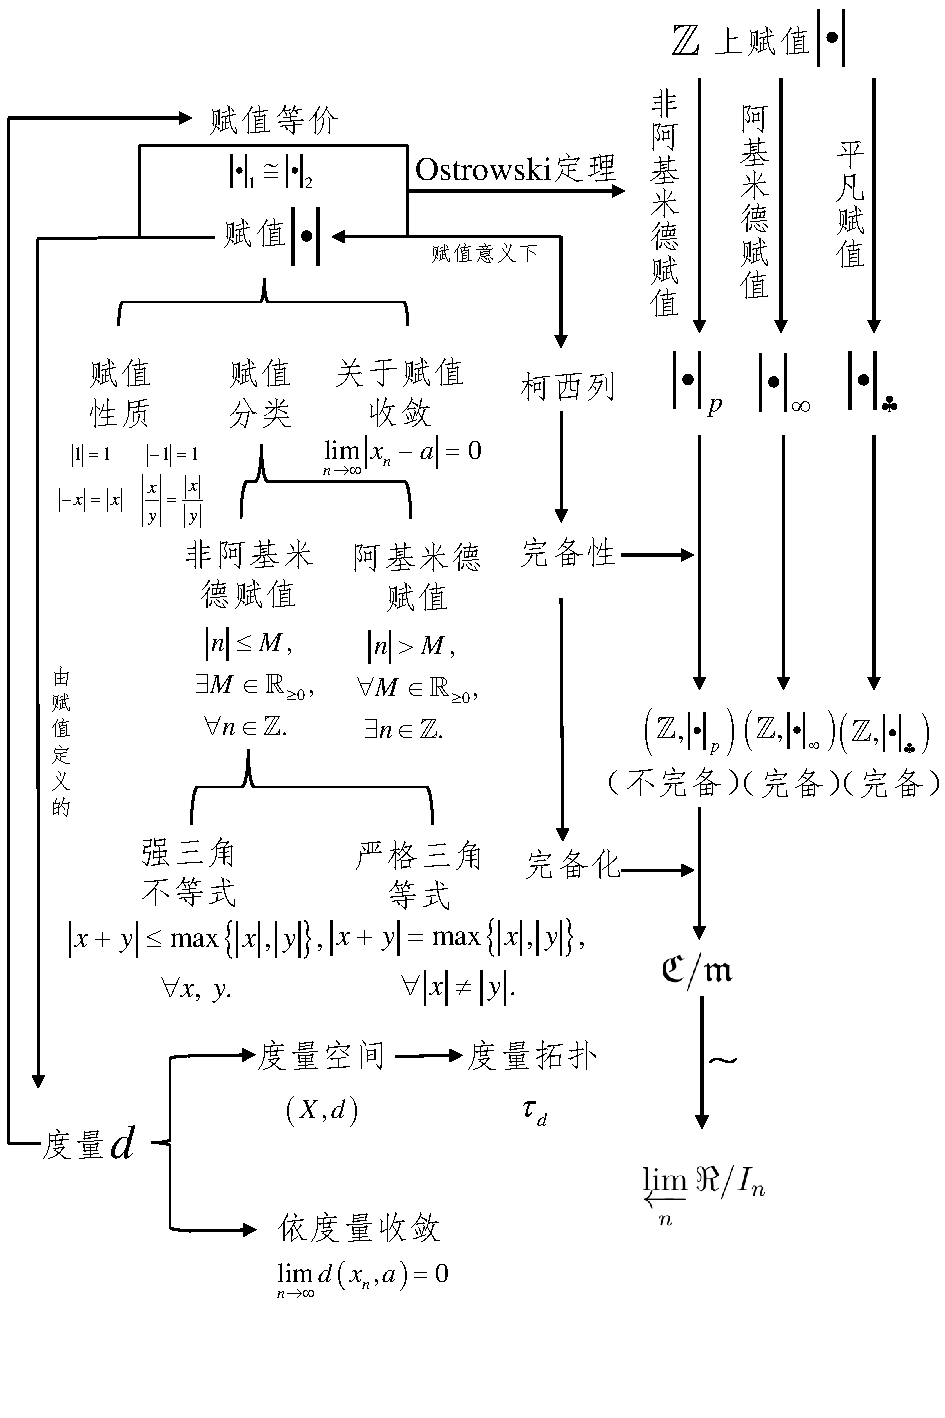
\includegraphics{likewise.pdf}
	
	% 进入Witt向量构造一节---------------------------------------------------------------------------------------
	\newpage
	\ 
	\newpage
	\section{Witt向量引入}
	\zihao{-4}
	\S~1节得到的$\varprojlim_n
	\mathbb{Z} /{{p}^{n}\mathbb{Z}}$中的每个元素是一个可数无穷序列${{\left( {{x}_{n}} \right)}_{n\in \mathbb{N}}}$, 代数结构比较清晰, 但是序列中任何两个不同的元素${{x}_{i}},\ {{x}_{j}}$包含了重叠的信息. 具体地说, 若$i\le j$, 则${{x}_{i}}$的所有信息都囊括于${{x}_{j}}$中. 于是我们首先寻求一种更典型的, 更精简的代数结构来表示$\left( \mathbb{Z},{{\left| \bigcdot  \right|}_{p}} \right)$的完备化. 这就是\S~2.1节的工作, 得到的精简结构为${{\mathbb{Z}}_{p}}$. 进一步地, 我们想要探索元素依然为可数无穷序列${{\left( {{y}_{n}} \right)}_{n\in \mathbb{N}}}$, 但是元素分量形式(或者规律)和环结构都与$\varprojlim_n
	\mathbb{Z} /{{p}^{n}\mathbb{Z}}$不同的另一种环结构, 使之与${{\mathbb{Z}}_{p}}$呈环同构, 从而拓展${{\mathbb{Z}}_{p}}$的表示方式. \S~2.2 节的工作就是为这种全新的代数结构作数学逻辑上的引入. \\
	\phantom{哈哈}
	
	\subsection{$\mathbb{Z}_p$表示法}
	\zihao{-4}
	选取$\mathbb{Z}$的一个双边理想降链
	\[
		\mathbb{Z}\supset p\mathbb{Z}\supset {{p}^{2}}\mathbb{Z}\supset \cdots ,
	\]
	存在相应的满射环同态
	\[
	\Re /{{I}_{1}}\xleftarrow{{{\lambda }_{1}}}\Re /{{I}_{2}}\xleftarrow{{{\lambda }_{2}}}\Re /{{I}_{3}}\xleftarrow{{{\lambda }_{3}}}\cdots ,
	\]
	并由此构造得到$\left( \mathbb{Z},{{\left| \bigcdot  \right|}_{p}} \right)$的一个完备化$\varprojlim_n
	\mathbb{Z} /{{p}^{n}\mathbb{Z}}	$. 源于$\lambda \left( {{x}_{n+1}} \right)={{x}_{n}}$, $n=1,\ 2,\ \cdots$的限制, $\varprojlim_n
	\mathbb{Z} /{{p}^{n}\mathbb{Z}}$中的每个元素位置在后的分量完全囊括了位置在前分量的信息. 一种形象化理解的方式是将可数无穷序列${{\left( {{x}_{n}} \right)}_{n\in \mathbb{N}}}\in \varprojlim_n
	\mathbb{Z} /{{p}^{n}\mathbb{Z}}$视为一种崭新的数, 记为$a$. $\left( {{x}_{n}} \right)$与$a$之间成立关系
	\[
		{{x}_{n}}=a\ \bmod {{p}^{n}},
	\]
	即有
	\begin{align*}
		{{x}_{1}}&=a\ \bmod p, \\ 
		{{x}_{2}}&=a\ \bmod {{p}^{2}}={{x}_{1}}+{{a}_{1}}p,\ 
		{{a}_{1}}\in \left\{ 0,\ 1,\ \cdots ,\ p-1 \right\}, \\ 
		{{x}_{3}}&=a\ \bmod {{p}^{3}}={{x}_{2}}+{{a}_{2}}{{p}^{2}}={{x}_{1}}+{{a}_{1}}p+{{a}_{2}}{{p}^{2}},\ 
		{{a}_{2}}\in \left\{ 0,\ 1,\ \cdots ,\ p-1\right\},\\ 
		&\cdots \cdots. 
	\end{align*}
	因此, 我们不妨缩小研究范围, 只考虑每个${{\left( {{x}_{n}} \right)}_{n\in \mathbb{N}}}\in \varprojlim_n
	\mathbb{Z} /{{p}^{n}\mathbb{Z}}$的第$\infty $个分量
	\footnote{更具体地说, 是考虑$\left( {{x}_{n}} \right)$的第$\infty$个分量的级数形式, 而非其求和结果. }
	, 即考虑以下集合
	\begin{align*}
		{{\mathbb{Z}}_{p}}:&=\left\{ \underset{n\to \infty }{\mathop{\lim }}\,{{x}_{n}}:
		\ {{\left( {{x}_{n}} \right)}_{n\in \mathbb{N}}}\in \varprojlim_n
		\mathbb{Z} /{{p}^{n}\mathbb{Z}} \right\}. \\ 
		& =\left\{ \sum\limits_{v=0}^{\infty }{{{a}_{v}}{{p}^{v}}}:
		\ {{a}_{v}}\in \left\{ 0,\ 1,\ \cdots ,\ p-1 \right\},\ \forall v\in \mathbb{N} \right\}.
	\end{align*}
	\vskip 0.5cm
	
	基于\S~1.3节得出的结果, ${{\mathbb{Z}}_{p}}$上的加法运算$\oplus $和乘法运算$\otimes $为
	\begin{align*}
		\sum\limits_{v=0}^{\infty }{{{a}_{v}}{{p}^{v}}}\oplus \sum\limits_{v=0}^{\infty }{{{b}_{v}}{{p}^{v}}}&:=\sum\limits_{v=0}^{\infty }{{{a}_{v}}{{p}^{v}}}+\sum\limits_{v=0}^{\infty }{{{b}_{v}}{{p}^{v}}}\ \bmod \left( \underset{n\to \infty }{\mathop{\lim }}\,{{p}^{v}} \right)=\sum\limits_{v=0}^{\infty }{\left( {{a}_{v}}+{{b}_{v}} \right){{p}^{v}}}, \\ 
		\sum\limits_{v=0}^{\infty }{{{a}_{v}}{{p}^{v}}}\otimes \sum\limits_{v=0}^{\infty }{{{b}_{v}}{{p}^{v}}}&:=\sum\limits_{v=0}^{\infty }{{{a}_{v}}{{p}^{v}}}\times \sum\limits_{v=0}^{\infty }{{{b}_{v}}{{p}^{v}}}\ \bmod \left( \underset{n\to \infty }{\mathop{\lim }}\,{{p}^{v}} \right)=\sum\limits_{v=0}^{\infty }{\left( \sum\limits_{i+j=v}^{{}}{{{a}_{i}}\times {{b}_{j}}} \right){{p}^{v}}},
	\end{align*}
	由此可见$\oplus ,\ \otimes $实质上分别就是平凡运算$+,\ \times $, 后续对二者不加区分. 此时更加典范的表达为
	\begin{align*}
		\sum\limits_{v=0}^{\infty }{{{a}_{v}}{{p}^{v}}}+\sum\limits_{v=0}^{\infty }{{{b}_{v}}{{p}^{v}}}&:=\sum\limits_{v=0}^{\infty }{{{c}_{v}}{{p}^{v}}},\ {{c}_{v}}=\left\{ \begin{gathered}
			 {{a}_{0}}+{{b}_{0}}\ \bmod p,
			 \ v=0, \\ 
			 \frac{1}{{{p}^{v}}}\left( \sum\limits_{k=0}^{v}{\left( {{a}_{k}}+{{b}_{k}} \right){{p}^{k}}}
			 \ \bmod {{p}^{v+1}}-\sum\limits_{k=0}^{v-1}{{{c}_{k}}{{p}^{k}}} \right),\ v>0.
		\end{gathered} \right. \\ 
		\sum\limits_{v=0}^{\infty }{{{a}_{v}}{{p}^{v}}}\times \sum\limits_{v=0}^{\infty }{{{b}_{v}}{{p}^{v}}}&:=\sum\limits_{v=0}^{\infty }{{{d}_{v}}{{p}^{v}}},\ {{d}_{v}}=\left\{ \begin{gathered}
			{{a}_{0}}\times {{b}_{0}}\ \bmod p,
			\ v=0, \\ 
			\frac{1}{{{p}^{v}}}\left( \sum\limits_{k=0}^{v}{\sum\limits_{i+j=k}^{{}}{{{a}_{i}}{{b}_{j}}}{{p}^{k}}}\ \bmod {{p}^{v+1}}-\sum\limits_{k=0}^{v-1}{{{d}_{k}}{{p}^{k}}} \right),\ v>0.
		\end{gathered} \right.
	\end{align*}
	显然$\left( {{\mathbb{Z}}_{p}},+,\times  \right)$是一个环结构. 而${{\mathbb{Z}}_{p}}$上的赋值${{\left| \bigcdot  \right|}_{\bigstar}}$为
	\[
		{{\left| \sum\limits_{v=0}^{\infty }{{{a}_{v}}{{p}^{v}}} \right|}_{\bigstar}}:=\underset{n\to \infty }{\mathop{\lim }}\,{{\left| \sum\limits_{v=0}^{n}{{{a}_{v}}{{p}^{v}}} \right|}_{p}}={{\left| \underset{n\to \infty }{\mathop{\lim }}\,\sum\limits_{v=0}^{n}{{{a}_{v}}{{p}^{v}}} \right|}_{p}}={{\left| \sum\limits_{v=0}^{\infty }{{{a}_{v}}{{p}^{v}}} \right|}_{p}},
	\]
	即${{\left| \bigcdot  \right|}_{\bigstar}}$实质上就是${{\left| \bigcdot  \right|}_{p}}$. 后续对二者不加区分. 对任意一个$a:=\sum_{v=0}^{\infty }{{{a}_{v}}{{p}^{v}}}\in {{\mathbb{Z}}_{p}}$, 记
	\begin{align*}
		\Lambda &:=\left\{ k\ge 0:\ {{a}_{k}}\ne 0 \right\}, \\ 
		m&:=\left\{ \begin{aligned}
			& \min \Lambda ,\ \Lambda \ne \varnothing , \\ 
			& \infty ,\ \Lambda =\varnothing . 
		\end{aligned} \right. 
	\end{align*}
	由于${{a}_{v}}\in \left\{ 0,\ 1,\ \cdots ,\ p-1 \right\}$, 因此有$\left. {{p}^{v}} \right\|{{a}_{v}}{{p}^{v}}$, 且由于${{\left| \bigcdot  \right|}_{p}}$是非阿基米德赋值, 根据推论\ref{强三角不等式推论3}, 则$a$的$p$-进赋值为
	\[
		{{\left| a \right|}_{p}}={{p}^{-m}}\in \left[ 0,1 \right].
	\]
	\vskip 0.5cm
	
	现在我们对${{\mathbb{Z}}_{p}}$能表示$\varprojlim_n \mathbb{Z} /{{p}^{n}\mathbb{Z}}$作严格的说明. 考虑映射$f$
	\[f:\ \begin{matrix}
		{{\mathbb{Z}}_{p}} & \to  & \varprojlim_n \mathbb{Z} /{{p}^{n}\mathbb{Z}}  \\
		\sum\limits_{v=0}^{\infty }{{{a}_{v}}{{p}^{v}}} & \to  & {{\left( \sum\limits_{v=0}^{n}{{{a}_{v}}{{p}^{v}}} \right)}_{n\in \mathbb{N}}}
	\end{matrix}.\]
	\begin{mingti} \label{Zp单射引理}
		设$n\in {{\mathbb{Z}}_{\ge 0}}$,\ $\sum_{v=0}^{n}{{{a}_{v}}{{p}^{v}}},
		\ \sum_{v=0}^{n}{{{b}_{v}}{{p}^{v}}}\in {{\mathbb{Z}}_{p}}$, 则成立
		\[
			\sum\limits_{v=0}^{n }{{{a}_{v}}{{p}^{v}}}=\sum\limits_{v=0}^{n}{{{b}_{v}}{{p}^{v}}}.
			\ \Longleftrightarrow \ 
			{{a}_{v}}={{b}_{v}},\ \forall v\in \left\{ 0,\ 1,\ \cdots,\ n \right\}.
		\]
	\end{mingti}
	\begin{proof}
		$\left( \Leftarrow  \right)$方向的推理是显然的, 因此只需要关注$\left( \Rightarrow  \right)$方向的推理. 
		若成立$\sum_{v=0}^{n }{{{a}_{v}}{{p}^{v}}}=\sum_{v=0}^{n }{{{b}_{v}}{{p}^{v}}}$, 则移项并合并同类项, 得到
		\begin{equation} \label{202102212248_1}
			\sum\limits_{v=0}^{n}{\left( {{a}_{v}}-{{b}_{v}} \right){{p}^{v}}}=:\sum\limits_{v=0}^{n }{{{c}_{v}}{{p}^{v}}}=0,\ {{c}_{v}}={{a}_{v}}-{{b}_{v}}.
		\end{equation}
		由于${{a}_{v}},\ {{b}_{v}}\in \left\{ 0,\ 1,\ \cdots,\ p-1 \right\}$, 因此有
		\begin{equation} \label{202102212248_3}
			{{c}_{v}}\in \left\{ -\left( p-1 \right),\ -\left( p-2 \right),\ \cdots,\ 0,\ 1,\ \cdots ,\ \left( p-2 \right),\ \left( p-1 \right) \right\},\ \forall v.
		\end{equation}
		\vskip 0.3cm
		\begin{itemize}
			\item 由式(\ref{202102212248_1}), 
			式(\ref{202102212248_3}), 有
			\begin{equation} \label{202102212248_2}
				{{c}_{0}}=-\left( {{c}_{1}}+\cdots +{{c}_{n}}{{p}^{n-1}} \right)p.
				\ \Longrightarrow \ 
				\left. p \right|{{c}_{0}}.
				\ \Longrightarrow \ 
				{{c}_{0}}=0.
			\end{equation}
			
			\item 由式(\ref{202102212248_1}), 
			式(\ref{202102212248_3}), 
			式(\ref{202102212248_2}), 有
			\begin{align*}
				&{{c}_{1}}p=-\left( {{c}_{2}}{{p}^{2}}+\cdots +{{c}_{n}}{{p}^{n}} \right)=-\left( {{c}_{2}}+\cdots +{{c}_{n}}{{p}^{n-2}} \right){{p}^{2}}. \\ 
				\Longrightarrow\ & {{c}_{1}}=-\left( {{c}_{2}}+\cdots +{{c}_{n}}{{p}^{n-2}} \right)p. \\ 
				\Longrightarrow\ & \left. p \right|{{c}_{1}}.\ \Longrightarrow \ {{c}_{1}}=0.
			\end{align*}
		
			\item \ldots \ldots.
		\end{itemize}
		\vskip 0.3cm
		重复以上操作, 即可得到
		\[
			\text{式(\ref{202102212248_1})成立.}
			\ \Longrightarrow\ 
			{{c}_{0}}={{c}_{1}}=\cdots ={{c}_{n}}=0.
		\]
		至此, 明所欲证.
	\end{proof}
	\begin{tuilun} \label{Zp单射推论}
		任取$\sum_{v=0}^{\infty }{{{a}_{v}}{{p}^{v}}},
		\ \sum_{v=0}^{\infty }{{{b}_{v}}{{p}^{v}}}\in {{\mathbb{Z}}_{p}}$, 成立
		\[
			\sum\limits_{v=0}^{\infty }{{{a}_{v}}{{p}^{v}}}=\sum\limits_{v=0}^{\infty }{{{b}_{v}}{{p}^{v}}}.
			\ \Longleftrightarrow \ 
			{{\left( {{a}_{n}} \right)}_{n\in \mathbb{N}}}={{\left( {{b}_{n}} \right)}_{n\in \mathbb{N}}}.
		\]
	\end{tuilun}
	\begin{proof}
		由于$\sum_{v=0}^{\infty }{{{a}_{v}}{{p}^{v}}},
		\ \sum_{v=0}^{\infty }{{{b}_{v}}{{p}^{v}}}\in {{\mathbb{Z}}_{p}}$,\
		于是在极限存在的前提下, 
		令命题\ref{Zp单射引理}中的$n \to \infty$即可得证.
	\end{proof}
	\vskip 0.5cm
	
	在此基础上, 若${{\mathbb{Z}}_{p}}$中
	\[
		\sum_{v=0}^{\infty }{{{a}_{v}}{{p}^{v}}}\ne \sum_{v=0}^{\infty }{{{b}_{v}}{{p}^{v}}}.
	\]
	由推论\ref{Zp单射推论}, $\exists k\ge 0$, ${{a}_{k}}\ne {{b}_{k}}$, 即有${{\left( {{a}_{n}} \right)}_{n\le k}}\ne {{\left( {{b}_{n}} \right)}_{n\le k}}$. 再根据命题\ref{Zp单射引理}, 成立$\sum_{v=0}^{k}{{{a}_{v}}{{p}^{v}}}\ne \sum_{v=0}^{k}{{{b}_{v}}{{p}^{v}}}$, 因此也就有
	\[
		{{\left( \sum_{v=0}^{n}{{{a}_{v}}{{p}^{v}}} \right)}_{n\in \mathbb{N}}}\ne {{\left( \sum_{v=0}^{n}{{{b}_{v}}{{p}^{v}}} \right)}_{n\in \mathbb{N}}}.
	\]
	于是映射$f$是一个单射. 另一方面, 显然成立
	\[
		f\left( \sum\limits_{v=0}^{\infty }{{{a}_{v}}{{p}^{v}}} \right)={{\left( \sum\limits_{v=0}^{n}{{{a}_{v}}{{p}^{v}}} \right)}_{n\in \mathbb{N}}},\ \forall {{\left( \sum\limits_{v=0}^{n}{{{a}_{v}}{{p}^{v}}} \right)}_{n\in \mathbb{N}}}\in \varprojlim_n \mathbb{Z} /{{p}^{n}\mathbb{Z}},\ \exists \sum\limits_{v=0}^{\infty }{{{a}_{v}}{{p}^{v}}}\in {{\mathbb{Z}}_{p}}.
	\]
	因此$f$是一个满射. 除此之外, $\forall a,\ b\in {{\mathbb{Z}}_{p}}$, $f$显然满足
	\begin{align*}
		f\left( a+b \right)&=f\left( a \right)+f\left( b \right), \\ 
		f\left( ab \right)&=f\left( a \right)f\left( b \right).
	\end{align*}
	于是我们导出了以下的定理. 
	\begin{dingli}
		${{\mathbb{Z}}_{p}}$是$\varprojlim_n \mathbb{Z} /{{p}^{n}\mathbb{Z}}$的环同构, 即有
		\[{{\mathbb{Z}}_{p}}\xrightarrow{\sim} \varprojlim_n \mathbb{Z} /{{p}^{n}\mathbb{Z}}.\]
	\end{dingli}
	\vskip 0.5cm
	
	最后, 我们通过对${{\mathbb{Z}}_{p}}$进行一些补充说明来结束此小节. 首先强调${{\mathbb{Z}}_{p}}$中的元素$\sum_{v=0}^{\infty }{{{a}_{v}}{{p}^{v}}}$并没有要求其部分和序列(在$\mathbb{Z}$中)收敛. 其次, ${{\mathbb{Z}}_{p}}$的构造超越了一些常识, 比如$\sum_{v=0}^{\infty }{{{p}^{v}}}$和$\sum_{v=0}^{\infty }{2{{p}^{v}}}$, 在实数域中它们都是发散的(或者说是不存在的), 都等于$\infty $. 而在${{\mathbb{Z}}_{p}}$中, 根据推论\ref{Zp单射推论}, 它们是存在且不相等的. 而对于整数环$\mathbb{Z}$嵌入${{\mathbb{Z}}_{p}}$的问题, 一方面, $\forall a\in {{\mathbb{Z}}_{\ge 0}}$, 显然可以通过一系列取模$p$算法将$a$表为具有形式
	$
		\sum\limits_{v=0}^{n}{{{a}_{v}}{{p}^{v}}}$,
		\ 
		${{a}_{v}}\in \left\{ 0,\ 1,\ \cdots ,\ p-1 \right\}
	$
	的有限和形式, 此时的嵌入是显然的:
	\[
		\begin{matrix}
			{{\mathbb{Z}}_{\ge 0}} & \hookrightarrow  & {{\mathbb{Z}}_{p}}  \\
			a & \to  & a  \\
		\end{matrix}.
	\]
	而对于$\forall \left( -a \right)\in {{\mathbb{Z}}_{<0}}$, 我们不能将其简单地表为$\sum_{v=0}^{\infty }{\left( -{{a}_{v}} \right){{p}^{v}}}$的形式, 因为此时$-{{a}_{v}}\le 0$, 该形式不被${{\mathbb{Z}}_{p}}$接纳. 对于非正整数的形式构造比较巧妙, 可见下面的例子. 
	\begin{lizi}
		$\mathbb{Z} \ni 0 \to 0+0\times p+0\times {{p}^{2}}+\cdots .$
	\end{lizi}
	\begin{lizi}
		$\mathbb{Z} \ni -1 \to \left( p-1 \right)+\left( p-1 \right)p+\left( p-1 \right){{p}^{2}}+\cdots =\sum_{v=0}^{\infty }{\left( p-1 \right){{p}^{v}}}.$
	\end{lizi}
	\begin{zhuji}
		\begin{align*}
			& -1=\left( p-1 \right)+\left( p-1 \right)p+\cdots +\left( p-1 \right){{p}^{n-1}}-{{p}^{n}}. \\ 
			\Longrightarrow\ & -1\equiv \left( p-1 \right)+\left( p-1 \right)p+\cdots +\left( p-1 \right){{p}^{n-1}}\ \bmod {{p}^{n}}. 
		\end{align*}
	\end{zhuji}
	\begin{lizi}
		$\mathbb{Q} \ni \frac{1}{1-p}\to 1+p+{{p}^{2}}+\cdots=\sum_{v=0}^{\infty }{{{p}^{v}}} .$
	\end{lizi}
	\begin{zhuji}
		\begin{align*}
			& 1=\left( 1+p+\cdots +{{p}^{n-1}} \right)\left( 1-p \right)+{{p}^{n}}. \\ 
			\Longrightarrow\ & \frac{1}{1-p}\equiv 1+p+\cdots +{{p}^{n-1}}\ \bmod {{p}^{n}}. 
		\end{align*}
	\end{zhuji}
	由$-a=a\times \left( -1 \right)$有以下嵌入
	\[\begin{matrix}
		{{\mathbb{Z}}_{\le 0}} & \hookrightarrow  & {{\mathbb{Z}}_{p}}  \\
		-a & \to  & a\times \sum\limits_{v=0}^{\infty }{\left( p-1 \right){{p}^{v}}}  \\
	\end{matrix}.\]
	
	%————————————————————————————————————————————————————
	\newpage
	\subsection{Witt向量的代数背景}
	\zihao{-4}
	在这一小节中, 我们先从\S~2.1节得到的代数结构${{\mathbb{Z}}_{p}}$出发, 一步步分析得到${{\mathbb{Z}}_{p}}$的另一种表示结构的初貌. 下面以${{\mathbb{Z}}_{p}}$的剩余环结构研究作为开始. 
	\begin{mingti} \label{Zp/pZp的等价表示}
		设$p$是一个素数.\ 存在以下环同构
		\[
			{{\mathbb{Z}}_{p}}/p{{\mathbb{Z}}_{p}}
			\xrightarrow{\sim}
			\mathbb{Z}/p\mathbb{Z}
			\xrightarrow{\sim}
			{{\mathbb{F}}_{p}}.
		\]
	\end{mingti}
	\begin{proof}
		关于后半部分的同构$\mathbb{Z}/p\mathbb{Z}
		\xrightarrow{\sim} 
		{{\mathbb{F}}_{p}}$是显然的,\ 详细说明可参见李文威\cite[例~5.2.4]{liwenwei}.\ 我们只需要说明前半部分的同构${{\mathbb{Z}}_{p}}/p{{\mathbb{Z}}_{p}}
		\xrightarrow{\sim}
		\mathbb{Z}/p\mathbb{Z}$即可.\ 
		\begin{align*}
			p{{\mathbb{Z}}_{p}}&=\left\{ \sum\limits_{v=1}^{\infty }{{{b}_{v}}{{p}^{v}}}:\ {{b}_{v}}\in \left\{ 0,\ 1,\ \cdots,\ p-1 \right\},
			\ \forall v\in {{\mathbb{Z}}_{\ge 1}} \right\}. \\ 
			&=\left\{ b\in {{\mathbb{Z}}_{p}}:
			\ {{\left| b \right|}_{p}}<1 \right\}
			\subset \mathbb{Z}_p. 
		\end{align*}
		显然是${{\mathbb{Z}}_{p}}$的一个理想,\ ${{\mathbb{Z}}_{p}}/p{{\mathbb{Z}}_{p}}$是一个剩余类环,\ 其结构可表示为
		\begin{align*}
			& {{\mathbb{Z}}_{p}}/p{{\mathbb{Z}}_{p}}\\
			=&\left\{ a+p{{\mathbb{Z}}_{p}}:\ a\in {{\mathbb{Z}}_{p}} \right\} \\ 
			=&\left\{ \left\{ \begin{gathered}
				 {{a}_{0}}+\sum\limits_{v=1}^{\infty }{{{b}_{v}}{{p}^{v}}}: \\ 
				 {{b}_{v}}\in \left\{ 0,\  1,\ \cdots ,\   p-1  \right\},\ \forall v\in {{\mathbb{Z}}_{\ge 1}} 
			\end{gathered} \right\}:\ {{a}_{0}}\in \left\{ 0,\  1,\ \cdots ,\   p-1  \right\} \right\}.
		\end{align*}
		仿$\mathbb{Z}/p\mathbb{Z}=\left\{ \widehat{0},\ \widehat{1},\ \cdots ,\ \widehat{\left( p-1 \right)} \right\}$, 可记${{\mathbb{Z}}_{p}}/p{{\mathbb{Z}}_{p}}=\left\{ \overline{0},\ \overline{1},\ \cdots ,\ \overline{\left( p-1 \right)} \right\}$, 其中
		$\overline{k}:=\left\{ k+\sum_{v=1}^{\infty }{{{b}_{v}}{{p}^{v}}} \right\}$.
		显然${{\mathbb{Z}}_{p}}/p{{\mathbb{Z}}_{p}}$与存在环同构$\phi $
		\[
			\phi :\ \begin{matrix}
				{{\mathbb{Z}}_{p}}/p{{\mathbb{Z}}_{p}} & \xrightarrow{\sim}  & \mathbb{Z}/p\mathbb{Z}  \\
				\overline{a} & \mapsto  & \widehat{a}  \\
			\end{matrix}.
		\]
		至此, 明所欲证.
	\end{proof}
	\vskip 0.5cm
	
	基于${{\mathbb{Z}}_{p}}$模去$p{{\mathbb{Z}}_{p}}$的剩余类环可视为特征为$p$的有限域${{\mathbb{F}}_{p}}$,\ 我们可选定某一映射$\tau :\ {{\mathbb{F}}_{p}}\to {{\mathbb{Z}}_{p}}$使得$\forall x\in {{\mathbb{F}}_{p}}$,\ $\tau \left( x \right)\equiv x\left( \bmod\ p{{\mathbb{Z}}_{p}} \right)$
	\footnote{$\tau \left( x \right)\equiv x\left( \bmod\ p{{\mathbb{Z}}_{p}} \right)$表示$\tau \left( x \right)+p{{\mathbb{Z}}_{p}}=x.$}
	,\ 
	称$\tau \left( x \right)$为$x$的一个提升.\ 提升的严格数学定义如下.\ 
	\begin{dingyi} \label{提升定义}
		设$\Re $是一个环,\ $\mathfrak{a}$是$\Re $的一个(双边)理想,\ 称映射$\tau $为剩余类环$\Re /\mathfrak{a}$到环$\Re $的一个{\heiti 提升}\index{提升},\ 若$\tau $满足
		\[
			\tau \left( x \right)\equiv x\text{ }\bmod \mathfrak{a},
			\ \forall x\in \Re /\mathfrak{a}.
		\]
	\end{dingyi}
	\begin{mingti} \label{提升存在性}
		设$\Re $是一个环,\ $\mathfrak{a}$是$\Re $的一个(双边)理想,\ 则剩余类环$\Re /\mathfrak{a}$到环$\Re $的提升$\tau $一定存在.\ 
	\end{mingti}
	\begin{proof}
		由于代表模去理想的映射$\phi :\ \Re \to \Re /\mathfrak{a}$是一个满射,\ 因此总是存在${{\Re }_{x}}$, 成立
		\[
			\phi \left( {{\Re }_{x}} \right)=x,
			\ \varnothing \ne {{\Re }_{x}}\subseteq \Re ,
			\ \forall x\in \Re /\mathfrak{a}.
		\]
		遍历$\Re /\mathfrak{a}$中的元素$x$,\ 任取${{r}_{x}}\in {{\Re }_{x}}$,\ 令$\tau \left( x \right):={{r}_{x}}$. 成立以下推理
		\[
		\left. \begin{aligned}
			{{r}_{x}}+\mathfrak{a}=\tau \left( x \right).\ &\Longrightarrow \ \tau \left( x \right)\equiv {{r}_{x}}\ \bmod \mathfrak{a}. \\ 
			\phi \left( {{r}_{x}} \right)={{r}_{x}}+\mathfrak{a}=x.
			\ &\Longrightarrow \ {{r}_{x}}\equiv x
			\ \bmod \mathfrak{a}.
		\end{aligned} \right\}\Longrightarrow \tau \left( x \right)\equiv x\ \bmod \mathfrak{a},\ \forall x\in \Re /\mathfrak{a}.	
		\]
		至此我们便构造得到了一个提升$\tau $,\ 其存在性得证.
	\end{proof}
	\vskip 0.5cm
	
	事实上,\ 在命题\ref{Zp/pZp的等价表示}给出的同构下,\ 不妨记
	\[
		{{\mathbb{F}}_{p}}=\left\{ \overline{0},\ \overline{1},\ \cdots ,\ \overline{\left( p-1 \right)} \right\},
	\]
	提升$\tau$的选取只需符合以下形式
	\[
		\tau :\ \begin{matrix}
			{{\mathbb{F}}_{p}} & \mapsto  & {{\mathbb{Z}}_{p}}  \\
			\overline{a} & \to  & \begin{aligned}
				\text{任意选定的}{{a}_{0}}&\text{满足} \\ 
				{{a}_{0}}\equiv a\ \bmod&\ p. 
			\end{aligned}
		\end{matrix}
	\]
	由此我们得到了以下的一个交换图
	\[
		\xymatrix{
	\mathbb{Z}_p \ar@/^/[r]^{\phi:\ \text{模去}p\mathbb{Z}_p} &
	\mathbb{F}_p \ar@/^/[l]^{\tau:\ \text{提升}}	
	}
	\]
	现任意取定一个提升$\tau$,\ 进行以下操作.\ 
	\begin{suanfa} \label{suanfa3.3}
	\ 
	\begin{itemize}
		\item $\forall \widetilde{x}\in {{\mathbb{Z}}_{p}}$,\ 记${{x}_{0}}=\phi \left( \widetilde{x} \right)\in {{\mathbb{F}}_{p}}$,\ 则$\exists \widetilde{{{x}_{1}}}\in {{\mathbb{Z}}_{p}}$使得$\widetilde{x}=\tau \left( {{x}_{0}} \right)+p\widetilde{{{x}_{1}}}.$
		
		\item 记${{x}_{1}}=\phi \left( \widetilde{{{x}_{1}}} \right)$,\ 则$\exists \widetilde{{{x}_{2}}}\in {{\mathbb{Z}}_{p}}$使得$\widetilde{{{x}_{1}}}=\tau \left( {{x}_{1}} \right)+p\widetilde{{{x}_{2}}}.$
		
		\item \ldots\ldots.
	\end{itemize}
	\end{suanfa}
	\vskip 0.5cm
	
	由此得到一个序列${{x}_{0}},\ {{x}_{1}},\ \cdots $,\ 使得$\forall n\ge 0$,\ 成立
	\begin{align*}
		\widetilde{x}&=\tau \left( {{x}_{0}} \right)+p\widetilde{{{x}_{1}}} \\ 
		& =\tau \left( {{x}_{0}} \right)+p\left( \tau \left( {{x}_{1}} \right)+p\widetilde{{{x}_{2}}} \right) \\ 
		& =\cdots \\
		& =\tau \left( {{x}_{0}} \right)+\tau \left( {{x}_{1}} \right)p+\cdots +\tau \left( {{x}_{n}} \right){{p}^{n}}+\widetilde{{{x}_{n+1}}}{{p}^{n+1}},\text{ }\widetilde{{{x}_{n+1}}}\in {{\mathbb{Z}}_{p}}.
	\end{align*}
	令$n\to \infty $,\ 即可得
	\begin{equation} \label{Zp元素的级数表示}
		\widetilde{x}=\tau \left( {{x}_{0}} \right)+\tau \left( {{x}_{1}} \right)p+\cdots +\tau \left( {{x}_{n}} \right){{p}^{n}}+\cdots=\sum\limits_{n=0}^{\infty }{\tau \left( {{x}_{n}} \right){{p}^{n}}}.
	\end{equation}
	显然由上面操作得到的无穷级数$\sum_{n=0}^{\infty }{\tau \left( {{x}_{n}} \right){{p}^{n}}}$在${{\mathbb{Z}}_{p}}$中收敛到$\widetilde{x}$.\ 针对算法\ref{suanfa3.3}有下面的命题.\ 
	\begin{mingti} \label{202102161623_1}
		$\forall \widetilde{x}\in {{\mathbb{Z}}_{p}}$,\ 满足式(\ref{Zp元素的级数表示})的序列
		$\left( {{x}_{0}},\ {{x}_{1}},\ \cdots ,\ {{x}_{n}},\ \cdots  \right)$
		是存在且唯一的.\ 
	\end{mingti}
	\begin{proof}
		任意取定一个$\widetilde{x}\in {{\mathbb{Z}}_{p}}$,\ 首先可以确定${{x}_{0}}=\phi \left( \widetilde{x} \right)$是存在且唯一的.\ 
		
		运算$\phi $的实质就是取模运算${{x}_{0}}=\widetilde{x}+p{{\mathbb{Z}}_{p}}\in {{\mathbb{F}}_{p}}$,\ 即有
		\[
			\widetilde{x}\equiv {{x}_{0}}\ \bmod p{{\mathbb{Z}}_{p}}.
		\]
		提升$\tau $的定义\ref{提升定义}蕴涵
		\[
			{{x}_{0}}\equiv \tau \left( {{x}_{0}} \right)\ \bmod p{{\mathbb{Z}}_{p}}.
		\]
		因此由同余式的传递性,\ 成立
		\begin{subequations} \label{202103060909}
			\begin{align}
			& \widetilde{x}\equiv \tau \left( {{x}_{0}} \right)\ \bmod p{{\mathbb{Z}}_{p}}. 
			\label{202103060909_1}
			\\ 
			\Longrightarrow\ & \widetilde{x}-\tau \left( {{x}_{0}} \right)\equiv 0\ \bmod p{{\mathbb{Z}}_{p}}. \\ 
			\Longrightarrow\ & \left. p \right|\widetilde{x}-\tau \left( {{x}_{0}} \right). 
			\end{align}
		\end{subequations}
		因此$\exists \widetilde{{{x}_{1}}}\in {{\mathbb{Z}}_{p}}$, 使得
		\begin{equation} \label{202103041026}
		\widetilde{x}=\tau \left( {{x}_{0}} \right)+p\widetilde{{{x}_{1}}}.
		\end{equation}
		假设存在另一个$\widetilde{{{x}_{1}}}'\in {{\mathbb{Z}}_{p}}$也成立$\widetilde{x}=\tau \left( {{x}_{0}} \right)+p\widetilde{{{x}_{1}}}'$, 则有
		\[
			p\widetilde{{{x}_{1}}}=p\widetilde{{{x}_{1}}}'.\ \Longrightarrow \ p\left( \widetilde{{{x}_{1}}}-\widetilde{{{x}_{1}}}' \right)=0.
		\]
		由于$\mathbb{Z}\subset {{\mathbb{Z}}_{p}}$,\ $\textup{char}\left( {{\mathbb{Z}}_{p}} \right)=\textup{char}\left( \mathbb{Z} \right)=0$,\ 素数$p$非整环$\mathbb{Z}_p$的零元,\ 因此即有
		\[\widetilde{{{x}_{1}}}-\widetilde{{{x}_{1}}}'=0.\ \Longrightarrow \ 
		\widetilde{{{x}_{1}}}=\widetilde{{{x}_{1}}}',\]
		即满足式(\ref{202103041026})的$\widetilde{{{x}_{1}}}$是存在且唯一的.
		因此${{x}_{1}}=\phi \left( \widetilde{{{x}_{1}}} \right)$也是存在且唯一的.\ 继续推导下去可得${{x}_{2}},{{x}_{3}},\cdots $也是存在且唯一的.\ 
	\end{proof}
	\vskip 0.5cm
	
	此外,\ 我们指出${{\mathbb{F}}_{p}}$中的任意序列${{\left( {{x}_{n}} \right)}_{n\ge 0}}$也能唯一确定一个$\widetilde{x}=\sum_{n=0}^{\infty }{\tau \left( {{x}_{n}} \right){{p}^{n}}}\in {{\mathbb{Z}}_{p}}$.\ 
	\begin{yinli} \label{yinli_202102141524}
		设$\Re $是一个环, $\left| \bigcdot  \right|$是$\Re $上的一个非阿基米德赋值, 且$\Re $关于赋值$\left| \bigcdot  \right|$是完备的, 则无穷级数$\sum_{i=1}^{\infty }{{{a}_{i}}}$在$\Re $中关于赋值$\left| \bigcdot  \right|$收敛的充要条件是
		\[
			\underset{i\to \infty }{\mathop{\lim }}\,\left| {{a}_{i}} \right|=0.
		\]
	\end{yinli}
	\begin{proof}
		记${{A}_{n}}=\sum_{i=1}^{n}{{{a}_{i}}}.$
		\begin{enumerate} % 从这里开始改.
			\item 若$\sum_{i=1}^{\infty }{{{a}_{i}}}$在$\Re $中关于赋值$\left| \bigcdot  \right|$收敛, 设收敛到$A$, 即$\lim_{n\to \infty }\left| {{A}_{n}}-A \right|=0$, 则成立
			\begin{align*}
				0\le \left| {{a}_{n}} \right|=\left| {{A}_{n+1}}-{{A}_{n}} \right|&=\left| \left( {{A}_{n+1}}-A \right)+\left( A-{{A}_{n}} \right) \right| \\ 
				& \le \left| {{A}_{n+1}}-A \right|+\left| {{A}_{n}}-A \right|\to 0\ \left( n\to \infty  \right),
			\end{align*}
			即成立$\lim_{i\to \infty }\left| {{a}_{i}} \right|=0$. 
			\vskip 0.3cm
			
			\item 若成立$\lim_{i\to \infty }\left| {{a}_{i}} \right|=0$, 则$\forall \varepsilon >0$, $\exists N\in \mathbb{N}$, 使得
			\[
				{{\left| \left| {{a}_{i}} \right|-0 \right|}_{\infty }}=\left| {{a}_{i}} \right|<\varepsilon ,\ \forall i\ge N.
			\]
			由于$\left| \bigcdot  \right|$具有非阿基米德性, 根据推论\ref{强三角不等式推论}, 成立
			\[
				\left| {{A}_{j}}-{{A}_{i}} \right|=\left| {{a}_{i+1}}+{{a}_{i+2}}+\cdots +{{a}_{j}} \right|\le \underset{i+1\le k\le j}{\mathop{\max }}\,\left\{ \left| {{a}_{k}} \right| \right\}<\varepsilon ,\ \forall j\ge i\ge N.
			\]
			从而部分和序列${{\left( {{A}_{n}} \right)}_{n\ge 0}}$是一个柯西列.\ 由于$\left( \Re ,{{\left| \bigcdot  \right|}_{p}} \right)$是完备的,\ 因此柯西列${{\left( {{A}_{n}} \right)}_{n\ge 0}}$在$\Re$中收敛,\ 
			即无穷级数$\sum_{i=1}^{\infty }{{{a}_{i}}}$在$\Re$中收敛.\ 
		\end{enumerate}
	\end{proof}
	\begin{mingti} \label{202102161623_2}
		${{\mathbb{F}}_{p}}$中的任意序列${{\left( {{x}_{n}} \right)}_{n\ge 0}}$对应的无穷级数$\widetilde{x}:=\sum_{n=0}^{\infty }{\tau \left( {{x}_{n}} \right){{p}^{n}}}$在$\left( {{\mathbb{Z}}_{p}},{{\left| \bigcdot  \right|}_{p}} \right)$中是收敛的.\ 
	\end{mingti}
	\begin{proof}
		由于
		\[
			0\le {{\left| \tau \left( {{x}_{n}} \right){{p}^{n}} \right|}_{p}}\le {{p}^{-n}}\to 0\ \left( n\to \infty  \right),
		\]
		由极限的迫敛性,\ 成立
		\[
			\underset{n\to \infty }{\mathop{\lim }}\,{{\left| \tau \left( {{x}_{n}} \right){{p}^{n}} \right|}_{p}}=0.
		\]
		由于${{\mathbb{Z}}_{p}}$关于非阿基米德的$p$-进赋值${{\left| \bigcdot  \right|}_{p}}$是完备的,\ 根据引理\ref{yinli_202102141524},\ 无穷级数$\widetilde{x}$在${{\mathbb{Z}}_{p}}$中收敛.\ 
	\end{proof}
	\vskip 0.5cm
	
	于是由命题\ref{202102161623_1}和命题\ref{202102161623_2},\ 我们可以得到以下的一个集合双射$\Gamma_0 $
	\[\Gamma_0 :\ \begin{matrix}
		\prod\limits_{n\ge 0}^{{}}{{{\mathbb{F}}_{p}}} & \xrightarrow{1:1}  & {{\mathbb{Z}}_{p}}  \\
		x={{\left( {{x}_{n}} \right)}_{n\ge 0}} & \to  & \sum\limits_{n=0}^{\infty }{\tau \left( {{x}_{n}} \right){{p}^{n}}}  
	\end{matrix}\]
	由于$\Gamma_0 $是双射,\ 因此存在同是双射的逆映射${{\Gamma_0 }^{-1}}:\ {{\mathbb{Z}}_{p}}\to \prod_{n\ge 0}^{{}}{{{\mathbb{F}}_{p}}}$.\ 至此我们完成了将环$\left( {{\mathbb{Z}}_{p}},+,\bigcdot  \right)$中的元素一一投影到$\prod_{n\ge 0}^{{}}{{{\mathbb{F}}_{p}}}$中.\ 若能进一步定义$\prod_{n\ge 0}^{{}}{{{\mathbb{F}}_{p}}}$上的运算$\oplus $和$\odot $使之成为一个环,\ 并且保证映射$\Gamma_0 $满足
	\begin{align*}
		\Gamma_0  \left( x\oplus y \right)&=\Gamma_0  \left( x \right)+\Gamma_0  \left( y \right), \\ 
		\Gamma_0  \left( x\odot y \right)&=\Gamma_0  \left( x \right)\bigcdot \Gamma_0  \left( y \right), 
	\end{align*}
	则$\Gamma_0 $便是一个环同构,\ ${{\mathbb{Z}}_{p}}$的环结构也就可以体现在$\prod_{n\ge 0}^{{}}{{{\mathbb{F}}_{p}}}$上了,\ 此时$\prod_{n\ge 0}^{{}}{{{\mathbb{F}}_{p}}}$就是${{\mathbb{Z}}_{p}}$的一个表示.\ 
	\vskip 0.5cm
	
	上面是从环${{\mathbb{Z}}_{p}}$开始进行分析和推导的,\ 最终得到了一个从$\prod_{n\ge 0}^{{}}{{{\mathbb{F}}_{p}}}$到${{\mathbb{Z}}_{p}}$的双射结构$\Gamma_0$.\ 事实上,\ 这个分析过程只是一种特殊情况,\ 而囊括于更为广泛的一种代数现象.\ 下面我们先介绍几个相关的代数概念.\ 
	\begin{dingyi}
		设$p$是一个素数,\ $\left( \Re ,+,\bigcdot  \right)$是一个特征为$p$的环,\ 称$\Re ${\heiti (关于特征$p$)是完全的}\index{完全的}或者是一个{\heiti 完全环}\index{完全环},\ 若$\Re $上的自同态
		\[
			\textup{Fr}_p:\ \begin{matrix}
				\Re  & \mapsto  & \Re   \\
				x & \mapsto  & {{x}^{p}} 
			\end{matrix}
		\]
		是$\Re $上的自同构,\ 即$\textup{Fr}_p$是一个双射,\ 
		其中$x^p$表示
		\[
			\underbracket{x \bigcdot x \bigcdot \cdots \bigcdot x}_{p\text{个}}.
		\]
	\end{dingyi}
	\begin{zhuji}
		$\textup{Fr}_p$确实是一个环同态.\ 
			一方面,\ 显然有$\textup{Fr}_p\left( xy \right)={{\left( xy \right)}^{p}}={{x}^{p}}{{y}^{p}}=\textup{Fr}_p\left( x \right)\textup{Fr}_p\left( y \right)$;\ 另一方面,\ 由于$\Re $的特征为$p$,\ 故成立$\textup{Fr}_p\left( x+y \right)={{\left( x+y \right)}^{p}}={{x}^{p}}+{{y}^{p}}=\textup{Fr}_p\left( x \right)+\textup{Fr}_p\left( y \right)$. 
	\end{zhuji}
	\begin{lizi}
		有限域${{\mathbb{F}}_{p}}$是完全的.\ 
	\end{lizi}
	\begin{zhuji}
		推导过程涉及域上不可约多项式的一些知识,\ 此处略过,\ 详见李文威\cite[推论8.4.16]{liwenwei}.\ 
	\end{zhuji}
	\vskip 0.5cm
	
	完全环$\Re $具有以下的性质.\ 
	\begin{mingti} \label{mingti_3.1.6}
		设$\Re $是一个特征为$p$的完全环,\ 则$\forall x\in \Re $,\ $x$的$p$次根在$\Re $中是存在且唯一的,\ 记为${{x}^{{{p}^{-1}}}}$.
	\end{mingti}
	\begin{proof}
		由于环$\Re $是完全的,\ 因此$\Re $上的自同态
		$\textup{Fr}_p$
		是一个双射,\ $\textup{Fr}_p$可逆且逆映射${\textup{Fr}_p}^{-1}$也是一个双射.\ 因此$\forall x\in \Re $,\ $\exists !y\in \Re $满足$y={\textup{Fr}_p}^{-1}\left( x \right)$,\ 也就有
		\[
			{{y}^{p}}=\textup{Fr}_p\left( y \right)=\textup{Fr}_p\left( {\textup{Fr}_p}^{-1}\left( x \right) \right)=x.
		\]
		因此$y$是$x$在$\Re $中的唯一一个$p$次根.\ 
	\end{proof}
	\begin{tuilun} \label{完全环幂次根存在性}
		设$\Re $是一个特征为$p$的完全环,\ 则$\forall x\in \Re $,\ $\forall n\in {{\mathbb{Z}}_{\ge 0}}$,\ $x$的${{p}^{n}}$次根在$\Re $中是存在且唯一的,\ 记为${{x}^{{{p}^{-n}}}}$.\ 
	\end{tuilun}
	\begin{proof}
		\ 
		\begin{itemize}
			\item $n=0$时,\ $x$的${{p}^{n}}=1$次根就是$x$,\ 显然是唯一的.\ 
			
			\item $n=1$的情况已由命题\ref{mingti_3.1.6}给出.\ 
			
			\item $n>1$时,\ 由命题\ref{mingti_3.1.6},\ $\forall {{x}_{0}}\in \Re $,\ $\exists !{{x}_{1}}\in \Re $使得${{x}_{1}}^{p}=x$.\ 而对于${{x}_{1}}$,\ 同样地,\ $\exists !{{x}_{2}}\in \Re $使得${{x}_{2}}^{p}={{x}_{1}}$.\ 重复此过程,\ 可以得到
			\[
				\underbracket{{\left( {{\left( {{\left( {{x}_{n}} \right)}^{p}} \right)}^{p}}\cdots  \right)}^{p}}
				_{n\text{层嵌套}}=x
				\ \Longrightarrow \ 
				{{x}_{n}}^{{{p}^{n}}}=x.
			\]
			即${{x}_{n}}$是$x$在$\Re $中唯一一个${{p}^{n}}$次根.
		\end{itemize}
	\end{proof}
	\vskip 0.5cm
	
	有了完全环的概念基础,\ 现在我们就可以引入$p$-环的相关概念如下.\ 
	\begin{dingyi}
		设$\Re $为一个含幺交换环,\ 给定$\Re $的一个双边理想降链
		\[
			\Re ={{\mathfrak{a}}_{0}}\supset {{\mathfrak{a}}_{1}}\supset {{\mathfrak{a}}_{2}}\supset \cdots,
		\]
		并设$p$是一个素数,\ 记
		\[
			\bm{p}:=\underbracket{\bm{1}+\bm{1}+\cdots+\bm{1}}_
			{p\text{个}},
		\]
		其中$\bm{1}$是环$\Re$的幺元.\ 称$\Re $是一个{\heiti $p$-环}\index{$p$-环},\ 若满足
		\begin{enumerate}
			\item 相应的拓扑使$\Re $成为一个完备的{\heiti Hausdorff拓扑环}
			\index{Hausdorff拓扑环},\ 即
			$\Re 
			\xrightarrow{\sim}
			\varprojlim_{n}\Re /{{\mathfrak{a}}_{n}};$
			
			\item 对每个$n,\ m$皆有${{\mathfrak{a}}_{n}}{{\mathfrak{a}}_{m}}\subseteq {{\mathfrak{a}}_{n+m}};$
			
			\item $\bm{p}\in {{\mathfrak{a}}_{1}}$且剩余环$\kappa :=\Re /{{\mathfrak{a}}_{1}}$是完全的.\ 
		\end{enumerate}
		特别地,\ 称$p$-环$\Re $是一个{\heiti 严格$p$-环}\index{严格$p$-环},\ 若额外满足
		\begin{enumerate}
			\item $\bm{p}$在$\Re $中非零因子,\ 即不存在
			$\lambda \in {{\Re }_{\ne 0}}$使得$\bm{p}\lambda =0$(蕴涵$\textup{char}\left( \Re  \right)\ne p$)$;$
			
			\item ${{\mathfrak{a}}_{n}}={{\bm{p}}^{n}}\Re.$
		\end{enumerate}
	\end{dingyi}
	\begin{zhuji}
		$p$-环定义的条件(3)中的$\bm{p}\in {{\mathfrak{a}}_{1}}$可以等价地改写为$\textup{char}\left( \kappa  \right)=p$. 事实上, 由于${{\mathfrak{a}}_{1}}$真包含于$\Re $, 因此$\textup{char}\left( \kappa  \right)>1$. 在此基础上可以成立以下的等价关系
		\[
			\bm{p}\in {{\mathfrak{a}}_{1}}.
			\ \xLongleftrightarrow{{\mathfrak{a}}_{1}\text{运算封闭性}} \ 
			\sum\limits_{i=1}^{p}{\left( \bm{1}+{{\mathfrak{a}}_{1}} \right)}=\sum\limits_{i=1}^{p}\bm{1}+\sum\limits_{i=1}^{p}{{{\mathfrak{a}}_{1}}}=\bm{p}+{{\mathfrak{a}}_{1}}={{\mathfrak{a}}_{1}}.
			\ \xLongleftrightarrow{\textup{char定义,\ }p\textup{素}} \ 
			\textup{char}\left( \kappa  \right)=p.
		\]
	\end{zhuji}
	\begin{lizi} \label{例子:Zp}
		$\mathbb{Z}_{p}$是一个严格$p$-环.\ 
	\end{lizi}
	\begin{proof}
		给定${{\mathbb{Z}}_{p}}$的一个理想降链
		\[
			{{\mathbb{Z}}_{p}}\supset p{{\mathbb{Z}}_{p}}\supset {{p}^{2}}{{\mathbb{Z}}_{p}}\supset \cdots .
		\]
		\begin{enumerate}
			\item 
			${{\mathbb{Z}}_{p}}\xrightarrow{\sim}\varprojlim_{n}\mathbb{Z}/{{p}^{n}}\mathbb{Z}\xrightarrow{\sim}\varprojlim_{n}\mathbb{Z}_{p}/{{p}^{n}}\mathbb{Z}_{p}$是一个完备的Hausdorff拓扑环.\ 
			
			\item
			$\forall n,\ m\ge 0$,\ $\left( {{p}^{n}}{{\mathbb{Z}}_{p}} \right)\left( {{p}^{m}}{{\mathbb{Z}}_{p}} \right)=\left( {{p}^{n}}{{p}^{m}} \right)\left( {{\mathbb{Z}}_{p}}{{\mathbb{Z}}_{p}} \right)={{p}^{n+m}}{{\mathbb{Z}}_{p}}.$
			
			\item
			剩余环${{\mathbb{Z}}_{p}}/p{{\mathbb{Z}}_{p}}\cong {{\mathbb{F}}_{p}}$是一个特征为$p$的域,\ 是完全的, 且显然有$p=p\bigcdot 1\in p{{\mathbb{Z}}_{p}}$.\ 
		\end{enumerate}
		因此$\mathbb{Z}_p$是一个$p$-环.\ 
		此外,\ 由于$\textup{char}\left( {{\mathbb{Z}}_{p}} \right)=0\neq p$,\ $p$不是整环${{\mathbb{Z}}_{p}}$中的零元
		(因此也非零因子), 因此$\mathbb{Z}_p$也是一个严格$p$-环.\ 
	\end{proof}
	\begin{lizi}
		${{\mathbb{F}}_{p}}$-代数${{\mathbb{F}}_{p}}\left[\!\left[ t \right]\!\right]$是一个$p$-环,\ 但不是一个严格$p$-环.\ 
	\end{lizi}
	\begin{proof}
		给定${{\mathbb{F}}_{p}}\left[\!\left[ t \right]\!\right]$的一个理想降链
		\[
			{{\mathbb{F}}_{p}}\left[\!\left[ t \right]\!\right]=\left( 1 \right)\supset \left( t \right)\supset \left( {{t}^{2}} \right)\supset \cdots ,
		\]
		其中$\left( {{t}^{n}} \right)$表示由${{t}^{n}}\in {{\mathbb{F}}_{p}}\left[\!\left[ t \right]\!\right]$生成的主理想.\ 由于${{\mathbb{F}}_{p}}\left[\!\left[ t \right]\!\right]$是一个含幺交换环,\ 幺元同${{\mathbb{F}}_{p}}$的幺元$\bm{1}$,\ 因此根据主理想表示的基本知识\cite[P66]{fengkeqin},\ 有
		\[
			\left( {{t}^{n}} \right)={{t}^{n}}{{\mathbb{F}}_{p}}\left[\!\left[ t \right]\!\right].
		\]
		\begin{enumerate}
			\item ${{\mathbb{F}}_{p}}\left[\!\left[ t \right]\!\right]\xrightarrow{\sim}
			\varprojlim_{n}{{\mathbb{F}}_{p}}\left[\!\left[ t \right]\!\right]/{{t}^{n}}{{\mathbb{F}}_{p}}\left[\!\left[ t \right]\!\right]$
			是一个完备的Hausdorff拓扑环.\ 
			
			\item $\forall n,\ m\ge 0$,\ 成立
			\[
				\left( {{t}^{n}} \right)\left( {{t}^{m}} \right)=\left( {{t}^{n}}{{\mathbb{F}}_{p}}\left[\!\left[ t \right]\!\right] \right)\left( {{t}^{m}}{{\mathbb{F}}_{p}}\left[\!\left[ t \right]\!\right] \right)=\left( {{t}^{n}}{{t}^{m}} \right)\left( {{\mathbb{F}}_{p}}\left[\!\left[ t \right]\!\right]{{\mathbb{F}}_{p}}\left[\!\left[ t \right]\!\right] \right)={{t}^{n+m}}{{\mathbb{F}}_{p}}\left[\!\left[ t \right]\!\right]=\left( {{t}^{n+m}} \right).
			\]
			
			\item 剩余环${{\mathbb{F}}_{p}}\left[\!\left[ t \right]\!\right]/t{{\mathbb{F}}_{p}}\left[\!\left[ t \right]\!\right]\cong {{\mathbb{F}}_{p}}$是一个特征为$p$的域,\ 是完全的. 而由于${{\mathbb{F}}_{p}}\subset {{\mathbb{F}}_{p}}\left[\!\left[ t \right]\!\right]$,\ $\textup{char}\left( {{\mathbb{F}}_{p}}\left[\!\left[ t \right]\!\right] \right)=\textup{char}\left( {{\mathbb{F}}_{p}} \right)=p$, 因此有
			$\bm{p}=\bm{0}=\sum_{n=1}^{\infty }{\bm{0}\bigcdot {{t}^{n}}}\in t{{\mathbb{F}}_{p}}\left[\!\left[ t \right]\!\right]$. \ 
		\end{enumerate}
		因此${{\mathbb{F}}_{p}}\left[\!\left[ t \right]\!\right]$是一个$p$-环.\ 
		而由于$\bm{p}$在${{\mathbb{F}}_{p}}\left[\!\left[ t \right]\!\right]$中是零元(自然也是一个零因子), 
		$\left( {{t}^{n}} \right)\ne \left\{ \bm{0} \right\}={\bm{0}^{n}}{{\mathbb{F}}_{p}}\left[\!\left[ t \right]\!\right]={{\bm{p}}^{n}}{{\mathbb{F}}_{p}}\left[\!\left[ t \right]\!\right]$,\ 
		因此${{\mathbb{F}}_{p}}\left[\!\left[ t \right]\!\right]$不构成一个严格$p$-环.
	\end{proof}
	\vskip 0.5cm
	
	有了$p$-环结构后,\ 我们可以从严格$p$-环$\Re$出发,\ 仿照本小节开头部分,\ 进行类似的推导.\ 
	还是记$\bm{p}:=\sum_{i=1}^{p}{\left( \bm{1}\in \Re  \right)}$.\ 
	$\Re$是严格$p$-环,\ 存在双边理想降链
	\[
		\Re \supset \bm{p}\Re \supset {{\bm{p}}^{2}}\Re \supset \cdots .
	\]
	$\Re $上元素投影到${\bm{p}}\Re$依然可以通过模去理想${{\bm{p}}\Re}$的方式得到,\ 我们仍可取映射$\phi $为
	\[\phi :\ \begin{matrix}
		\Re  & \to  & \Re/{\bm{p}}\Re   \\
		x & \to  & x+{{\bm{p}}\Re}  \\
	\end{matrix}\]
	而基于命题\ref{提升存在性}提供的提升存在性保证,\ 
	我们便可以取某一个${\bm{p}}\Re$到$\Re $的提升$\tau $,\ 并结合$\phi $构成以下的交换图
	\[
	\xymatrix{
		\Re \ar@/^/[r]^{\phi:\ \text{模去} \mathfrak{a}_{1}} &
		\Re/ {\bm{p}}\Re \ar@/^/[l]^{\tau:\ \text{提升}}	
	}
	\]
	接着,\ 仿算法\ref{suanfa3.3},\ 对任意$\widetilde{x}\in \Re $,\ 我们也可以得到一个序列$\left( {{x}_{n}} \right)\in \prod_{n\ge 0}^{{}}{\Re/{\bm{p}}\Re}$满足
	\begin{equation} \label{202102162102}
		\widetilde{x}=\sum\limits_{n=0}^{\infty }{\tau \left( {{x}_{n}} \right){{\bm{p}}^{n}}}.
	\end{equation}
	注意由于$\Re$是严格$p$-环,\ 蕴含$\bm{p}\ne \bm{0} \in \Re$.\ 
	仿命题\ref{202102161623_1}的证明过程,\ 我们也有相似的命题.\ 
	\begin{mingti} \label{202102221629_1}
		$\forall \widetilde{x}\in \Re $,\ 满足式(\ref{202102162102})的序列$\left( {{x}_{0}},\ {{x}_{1}},\ \cdots ,\ {{x}_{n}},\ \cdots  \right)$是存在且唯一的.\ 
	\end{mingti}
	\vskip 0.5cm
	
	由于严格$p$-环$\Re $是一个完备的Hausdorff环, 蕴含$\Re $对定义其上的广义$p$-进赋值${{\left| \bigcdot  \right|}_{\bm{p}}}$是完备的. 
	并且$\Re \xrightarrow{\sim} \varprojlim_n \Re /\bm{p}\Re $的环同构揭示了$\Re$中元素也可表为$\mathbb{Z}_p$中元素那样的级数结构. 因此
	基于引理\ref{yinli_202102141524}, 我们可以完全仿照命题\ref{202102161623_2}的证明过程, 得到下面的命题. 
	\begin{mingti} \label{202102221629_2}
		$\Re /\bm{p}\Re $中的任意序列${{\left( {{x}_{n}} \right)}_{n\ge 0}}$对应的无穷级数$\widetilde{x}:=\sum_{n=0}^{\infty }{\tau \left( {{x}_{n}} \right){{\bm{p}}^{n}}}$在$\left( \Re ,{{\left| \bigcdot  \right|}_{\bm{p}}} \right)$中是收敛的.
	\end{mingti}
	
	于是由命题\ref{202102221629_1}和命题\ref{202102221629_2}, 我们也可以得到以下的一个集合双射$\Gamma_0$
	\[\Gamma_0 :\ \begin{matrix}
		\prod\limits_{n\ge 0}^{{}}{\Re /\bm{p}\Re } & \xrightarrow{1:1}  & \Re   \\
		x={{\left( {{x}_{n}} \right)}_{n\ge 0}} & \to  & \sum\limits_{n=0}^{\infty }{\tau \left( {{x}_{n}} \right){{\bm{p}}^{n}}}
	\end{matrix}.\]
	
	至此, 我们引出了严格$p$-环的另一种表示方式的代数初貌
	: $\prod_{n\ge 0}^{{}}{\Re /\bm{p}\Re }$, 也就是下一节要介绍的Witt向量集.
	
	\newpage
	\ 
	\newpage
	\section{用$\prod_{n\ge 0}^{{}}{{{\mathbb{F}}_{p}}}$表示${{\mathbb{Z}}_{p}}$}
	\zihao{-4}
	在\S~2.2节的最后我们得到了严格$p$-环$\Re $的剩余类环序列集$\prod_{n\ge 0}^{{}}{\Re /\bm{p}\Re }$到$\Re $的一个集合双射
	\[\Gamma_0 :\ \begin{matrix}
		\prod\limits_{n\ge 0}^{{}}{\Re /\bm{p}\Re } & \xrightarrow{1:1}  & \Re   \\
		x={{\left( {{x}_{n}} \right)}_{n\ge 0}} & \to  & \sum\limits_{n=0}^{\infty }{\tau \left( {{x}_{n}} \right){{\bm{p}}^{n}}}
	\end{matrix}.\]
	而若要用$\prod_{n\ge 0}^{{}}{\Re /\bm{p}\Re }$来表示$\Re $, 即将$\left( \Re ,+,\bigcdot  \right)$的环结构体现在$\prod_{n\ge 0}^{{}}{\Re /\bm{p}\Re }$上, 则额外要求我们考虑
	\begin{description}
		\item[任务一]怎么赋予$\prod_{n\ge 0}^{{}}{\Re /\bm{p}\Re }$运算$\oplus ,\ \odot $使之成为一个环;
		
		\item[任务二]双射$\Gamma_0 $是否能够将环$\left( \prod_{n\ge 0}^{{}}{\Re /\bm{p}\Re },\oplus ,\odot  \right)$的结构线性地投射到$\left( \Re ,+,\bigcdot  \right)$上, 即双射$\Gamma_0 $能否成为一个环态射, 满足
		\begin{align*}
			\Gamma_0 \left( x\oplus y \right)&=\Gamma_0 \left( x \right)+\Gamma_0 \left( y \right), \\ 
			\Gamma_0 \left( x\odot y \right)&=\Gamma_0 \left( x \right)\bigcdot \Gamma_0\left( y \right). 
		\end{align*}
	\end{description}
	本节就是致力于完成这两个任务. 值得一提的是, 任务一与任务二本质上并非相互孤立. 同一个双射$\Gamma_0 $可能对$\prod_{n\ge 0}^{{}}{\Re /\bm{p}\Re }$上的一种环结构${\mathcal{R}_{1}}$构成环态射, 而对其上的另一种环结构${\mathcal{R}_{2}}$不构成环态射. 而观察$\Gamma_0 $的映射形式, 又可以指出$\Gamma_0 $的性质取决于提升$\tau $的选取. 因此本节的核心就是同时兼容地构建$\left( \prod_{n\ge 0}^{{}}{\Re /\bm{p}\Re },\oplus ,\odot  \right)$与选取提升$\tau $. 前者由\S~3.2节解决, 后者由\S~3.3节解决. 而\S~3.1节则是为后两节的论述引入前置性的概念基础.
	\\ \phantom{哈哈}
	
	\subsection{Witt多项式}
	\zihao{-4}
	下面先给出Witt多项式以及Witt向量的定义.\ 
	
	\begin{dingyi} \label{Witt多项式和向量的定义}
		设$\left( \kappa,+,\bigcdot \right)$是一个含幺环满足$\textup{char}\left( \kappa \right)=p$,\ 记
		\[
			\bm{\pi} = \underbracket{\bm{1}+\bm{1}+\cdots+\bm{1}}_{\pi \text{个}}
			\in \kappa,
		\]
		其中$\pi$是一个素数, $\bm{1}$是$\kappa$的幺元.\ 
		$X=\left( {{X}_{0}},{{X}_{1}},\cdots ,{{X}_{n}},\cdots \right)\in \prod_{n\ge 0}^{{}}{\kappa }$是一列可数的无穷序列.\ 称下面的多项式组
		\begin{align*}
			{{W}_{0}}\left( X,\ \pi \right)&={{X}_{0}}, \\ 
			{{W}_{1}}\left( X,\ \pi \right)&={{X}_{0}}^{\pi}+\bm{\pi}{{X}_{1}}, \\ 
			 {{W}_{2}}\left( X,\ \pi \right)&={{X}_{0}}^{{{\pi}^{2}}}+\bm{\pi}{{X}_{1}}^{\pi}+{{\bm{\pi}}^{2}}{{X}_{2}}, \\ 
			&\ \vdots  \\ 
			 {{W}_{n}}\left( X,\ \pi \right)&={{X}_{0}}^{{{\pi}^{n}}}+\bm{\pi}{{X}_{1}}^{{{\pi}^{n-1}}}+\cdots +{{\bm{\pi}}^{n}}{{X}_{n}}=\sum\limits_{i=0}^{n}{{{\bm{\pi}}^{i}}{{X}_{i}}^{{{\pi}^{n-i}}}}, \\ 
			&\ \vdots
		\end{align*}
		是
		{\heiti 由序列$X$导出的,\ 系数为$\pi$的Witt多项式组},\ 
		${W}_{n}\left( X,\ \pi \right)$是
		{\heiti 由序列$X$导出的,\ 系数为$\pi$的
			第$n+1$级Witt多项式}
		\index{Witt多项式}
		,\ 其中
		\[{{\bm{\pi}}^{i}}{{X}_{i}}^{{{\pi}^{n-i}}}=\left( \underbracket{\bm{\pi}\bigcdot \bm{\pi}\bigcdot \cdots \bigcdot \bm{\pi}}_{\pi\text{个}} \right)\bigcdot \left( \underbracket{{{X}_{i}}\bigcdot {{X}_{i}}\bigcdot \cdots \bigcdot {{X}_{i}}}_
		{\pi^{n-i}\text{个}} \right)\in \kappa.\]
		在不会混淆的情况下, 也可以将${{W}_{n}}\left( X,\pi  \right)$简记为${{W}_{n}}\left( X \right)$或者${{W}_{n}}$.
		称序列$X$为$\kappa$上的一个
		{\heiti Witt向量}\index{Witt向量}.\ 
		特别地,\ 称${{X}^{\left( n \right)}}=\left( {{X}_{0}},{{X}_{1}},\cdots ,{{X}_{n}} \right)$是
		{\heiti 长度为$n+1$的截断Witt向量}.\ 
	\end{dingyi}
	\begin{zhuji}
		\ 
		\begin{enumerate}
			\item 一般要求素数$\pi \ne p$, 否则由于$\bm{\pi} =\bm{0}\in \kappa$, 会出现${{W}_{0}}={{W}_{1}}={{W}_{2}}=\cdots ={{X}_{0}}$. 后文的叙述中没有给出说明的情况下,
			一般都默认$\pi \ne p$.
			
			\item 一般也要求$\kappa$是交换环, 免去考虑
			$\kappa$上乘法运算顺序的麻烦. 后面没有给出指明时, 默认$\kappa$是一个含幺交换环.
		\end{enumerate}
	\end{zhuji}
	\vskip 0.5cm
	
	对于含幺交换环$\kappa $上的任一个可数无穷序列$X=\left( {{X}_{0}},{{X}_{1}},\cdots ,{{X}_{n}},\cdots  \right)\in \prod_{n\ge 0}^{{}}{\kappa }$, 自身的指数运算由下面的定义给出.
	\begin{dingyi} \label{Witt向量指数运算}		
		${{X}^{m}}:=\left( {{X}_{0}}^{m},{{X}_{1}}^{m},\cdots ,{{X}_{n}}^{m},\cdots  \right)$, 其中
		\[
			{{X}_{n}}^{m}=\left\{ \begin{aligned}
				& \bm{1},\ m=0, \\ 
				& \prod\limits_{i=1}^{m}{{{X}_{n}}},
				m\in {{\mathbb{Z}}_{>0}}.
			\end{aligned} \right.
		\]
	\end{dingyi}
	\vskip 0.5cm
	
	基于定义\ref{Witt向量指数运算}给出的指数运算规则, 由任一个序列$X$导出的相邻一级Witt多项式满足下面的关系式.
	\begin{mingti} \label{Witt迭代式命题}
		${{W}_{n+1}}\left( X,\pi  \right)={{W}_{n}}\left( {{X}^{\pi }},\pi  \right)+{\bm{\pi }^{n+1}}{{X}_{n+1}}$.
	\end{mingti}
	\begin{proof}
		成立以下推理
		\begin{align*}
			& {{W}_{n}}\left( X,\pi  \right)=\sum\limits_{i=0}^{n}{{\bm{\pi }^{i}}{{X}_{i}}^{{{\pi }^{n-i}}}}. \\ 
			\Longrightarrow& {{W}_{n}}\left( {{X}^{\pi }},\pi  \right)=\sum\limits_{i=0}^{n}{{\bm{\pi }^{i}}{{\left( {{X}_{i}}^{\pi } \right)}^{{{\pi }^{n-i}}}}}=\sum\limits_{i=0}^{n}{{\bm{\pi }^{i}}{{\left( {{X}_{i}} \right)}^{{{\pi }^{\left( n+1 \right)-i}}}}}. \\ 
			\Longrightarrow& {{W}_{n}}\left( {{X}^{\pi }},\pi  \right)+{\bm{\pi }^{n+1}}{{X}_{n+1}}=\sum\limits_{i=0}^{n+1}{{\bm{\pi }^{i}}{{\left( {{X}_{i}} \right)}^{{{\pi }^{\left( n+1 \right)-i}}}}}={{W}_{n+1}}\left( X,\pi  \right).
		\end{align*}
		至此, 明所欲证.
	\end{proof}
	\vskip 0.5cm
	
	反过来, 导出的Witt多项式也可以通过逐步反解的方法来表示序列$X$的每一个分量${{X}_{i}}$. 更具体地, 
	记多项式环$Z':=\mathbb{Z}\left[ {\bm{\pi}^{-1}} \right]$, 
	显然有$\mathbb{Z}\subset Z'$. 
	有如下命题.
	\begin{mingti} \label{202102231630}
		$\forall i\in {{\mathbb{Z}}_{\ge 0}}$, $\exists \Phi_{i} \in Z'\left[ {{Y}_{0}},{{Y}_{1}},\cdots  \right]$, 使得
		\[
			{{X}_{i}}=\Phi_{i} \left( {{W}_{0}},{{W}_{1}},\cdots  \right).
		\]
	\end{mingti}
	\begin{proof}
		当$i=0$时, 显然有${{X}_{0}}={{W}_{0}}\in Z\left[ {{W}_{0}} \right]\subset Z'\left[ {{W}_{0}},{{W}_{1}},\cdots  \right]$.\\
		假设$X$的前$k$个分量均满足
		\[
			{{X}_{i}}={{\Phi }_{i}}\left( {{W}_{0}},{{W}_{1}},\cdots  \right),
			\ \exists {{\Phi }_{i}}\in Z'\left[ {{Y}_{0}},{{Y}_{1}},\cdots  \right],
			\ i=0,\ 1,\ \cdots ,\ k-1.
		\]
		则对于第$k+1$个分量${{X}_{k}}$, 由
		\[
		{{W}_{k}}={{X}_{0}}^{{\bm{\pi }^{k}}}+\pi {{X}_{1}}^{{{\pi }^{k-1}}}+\cdots +{\bm{\pi }^{k}}{{X}_{k}}	
		\]
		可以反解出
		\begin{align*}
			{{X}_{k}}&=-{\bm{\pi }^{-k}}\left( {{X}_{0}}^{{\bm{\pi }^{k}}}+\pi {{X}_{1}}^{{\bm{\pi }^{k-1}}}+\cdots +{{\pi }^{k-1}}{{X}_{k-1}}^{\pi } \right)+{\bm{\pi }^{-k}}{{W}_{k}}. \\ 
			& =-\left( {\bm{\pi }^{-k}}{{\Phi }_{0}}^{{\bm{\pi }^{k}}}+{\bm{\pi }^{-\left( k-1 \right)}}{{\Phi }_{1}}^{{{\pi }^{k-1}}}+\cdots +{\bm{\pi }^{-1}}{{\Phi }_{k-1}}^{\pi } \right)+{\bm{\pi }^{-k}}{{W}_{k}}. \\ 
			& =:{{\Phi }_{k}}.
		\end{align*}
		由${\bm{\pi }^{-1}},\ {\bm{\pi }^{-2}},\ \cdots ,\ {\bm{\pi }^{-k}};\ {{\Phi }_{0}},\ {{\Phi }_{1}},\ \cdots ,\ {{\Phi }_{k-1}};\ {{W}_{k}}\in Z'\left[ {{W}_{0}},{{W}_{1}},\cdots  \right]$和多项式环$Z'\left[ {{W}_{0}},{{W}_{1}},\cdots  \right]$的环运算封闭性, 可得${{\Phi }_{k}}\in Z'\left[ {{Y}_{0}},{{Y}_{1}},\cdots  \right]$. 至此, 由第二数学归纳法, 结论得证. 
	\end{proof}
	\begin{lizi}
		${{X}_{0}}={{W}_{0}}$.
	\end{lizi}
	\begin{lizi}
		${{X}_{1}}={\bm{\pi }^{-1}}\left( -{{W}_{0}}^{\pi }+{{W}_{1}} \right)=-{\bm{\pi }^{-1}}{{W}_{0}}^{\pi }+{\bm{\pi }^{-1}}{{W}_{1}}.$
	\end{lizi}
	\begin{lizi}
	${{X}_{2}}={\bm{\pi }^{-2}}\left( -\bm{\pi} {{X}_{1}}^{\pi }-{{X}_{0}}^{{{\pi }^{2}}}+{{W}_{2}} \right)=-{\bm{\pi }^{-\left( \pi +1 \right)}}{{\left( -{{W}_{0}}^{\pi }+{{W}_{1}} \right)}^{\pi }}-{\bm{\pi }^{-2}}{{W}_{0}}^{{{\pi }^{2}}}+{\bm{\pi }^{-2}}{{W}_{2}}.$
	\end{lizi}
	\vskip 0.5cm
	
	现在考虑由两个序列$X$和$Y$分别导出的两个Witt多项式组${{\left( {{W}_{n}}\left( X \right) \right)}_{n\ge 0}}$和${{\left( {{W}_{n}}\left( Y \right) \right)}_{n\ge 0}}$. 基于此, 我们对上面的命题\ref{202102231630}作一个推广.
	\begin{mingti}	\label{202102231727}
		$\forall \Phi \in \mathbb{Z}\left[ X,Y \right]$, 存在$ \left( {{\varphi }_{0}},{{\varphi }_{1}},\cdots ,{{\varphi }_{n}},\cdots  \right)$满足
		\[
			{{\varphi }_{i}}\in Z'\left[ {{X}_{0}},\cdots ,{{X}_{n}},\cdots ;{{Y}_{0}},\cdots ,{{Y}_{n}},\cdots  \right],
			\ \forall i\in {{\mathbb{Z}}_{\ge 0}},
		\]
		成立
		\[
			{{W}_{n}}\left( {{\varphi }_{0}},\cdots ,{{\varphi }_{n}},\cdots  \right)=\Phi \left( {{W}_{n}}\left( {{X}_{0}},\cdots  \right),{{W}_{n}}\left( {{Y}_{0}},\cdots  \right) \right),\ n=0,\ 1,\ \cdots .
		\]
	\end{mingti}
	\begin{proof}
		当$n=0$时, 成立${{W}_{0}}\left( {{\varphi }_{0}},\cdots ,{{\varphi }_{n}},\cdots  \right)=\Phi \left( {{W}_{0}}\left( {{X}_{0}},\cdots  \right),{{W}_{0}}\left( {{Y}_{0}},\cdots  \right) \right)$, 即有
		\[
			{{\varphi }_{0}}=\Phi \left( {{X}_{0}},{{Y}_{0}} \right)\in \mathbb{Z}\left[ {{X}_{0}},{{Y}_{0}} \right]\subset Z'\left[ {{X}_{0}},\cdots ,{{X}_{n}},\cdots ;{{Y}_{0}},\cdots ,{{Y}_{n}},\cdots  \right].
		\]
		假设对$\left( {{\varphi }_{n}} \right)$的前$k$个分量都成立${{\varphi }_{i}}\in Z'\left[ {{X}_{0}},\cdots ,{{X}_{n}},\cdots ;{{Y}_{0}},\cdots ,{{Y}_{n}},\cdots  \right]$, $i=0,\ 1,\ \cdots ,\ k-1$.  考虑第$k+1$个等式
		\begin{align*}
			& \sum\limits_{i=0}^{k}{{\bm{\pi }^{i}}{{\varphi }_{i}}^{{{\pi }^{k-i}}}}={{W}_{k}}\left( {{\varphi }_{0}},\cdots ,{{\varphi }_{k}} \right)=\Phi \left( {{W}_{k}}\left( {{X}_{0}},\cdots  \right),{{W}_{k}}\left( {{Y}_{0}},\cdots  \right) \right). \\ 
			\Longrightarrow\ & {\bm{\pi }^{k}}{{\varphi }_{k}}=\Phi \left( {{W}_{k}}\left( {{X}_{0}},\cdots  \right),{{W}_{k}}\left( {{Y}_{0}},\cdots  \right) \right)-\sum\limits_{i=0}^{k-1}{{\bm{\pi }^{i}}{{\varphi }_{i}}^{{{\pi }^{k-i}}}}. \\ 
			\Longrightarrow\ & {{\varphi }_{k}}={\bm{\pi }^{-k}}\Phi \left( {{W}_{k}}\left( {{X}_{0}},\cdots  \right),{{W}_{k}}\left( {{Y}_{0}},\cdots  \right) \right)-\sum\limits_{j=1}^{k}{{\bm{\pi }^{-j}}{{\varphi }_{-j+k}}^{{{\pi }^{j}}}}.
		\end{align*}
		根据
		\begin{align*}
			{\bm{\pi }^{-1}},\ {\bm{\pi }^{-2}},\ \cdots ,\ {\bm{\pi }^{-k}};\ {{\varphi }_{0}},\ {{\varphi }_{1}},\ \cdots ,\ {{\varphi }_{k-1}}&\in Z'\left[ {{X}_{0}},\cdots ,{{X}_{n}},\cdots ;{{Y}_{0}},\cdots ,{{Y}_{n}},\cdots  \right], \\ 
			\Phi \left( {{W}_{k}}\left( {{X}_{0}},\cdots  \right),{{W}_{k}}\left( {{Y}_{0}},\cdots  \right) \right)&=\Phi \left( {{X}_{0}},\cdots ,{{X}_{n}},\cdots ;{{Y}_{0}},\cdots ,{{Y}_{n}},\cdots  \right). \\ 
			&\in \mathbb{Z}\left[ {{X}_{0}},\cdots ,{{X}_{n}},\cdots ;{{Y}_{0}},\cdots ,{{Y}_{n}},\cdots  \right]. \\ 
			& \subset Z'\left[ {{X}_{0}},\cdots ,{{X}_{n}},\cdots ;{{Y}_{0}},\cdots ,{{Y}_{n}},\cdots  \right],
		\end{align*}
		和多项式环$Z'\left[ {{X}_{0}},\cdots ,{{X}_{n}},\cdots ;{{Y}_{0}},\cdots ,{{Y}_{n}},\cdots  \right]$的环运算封闭性, 得到
		\[
			{{\varphi }_{k}}\in Z'\left[ {{X}_{0}},\cdots ,{{X}_{n}},\cdots ;{{Y}_{0}},\cdots ,{{Y}_{n}},\cdots  \right].
		\]
		至此, 由第二数学归纳法, 结论得证. 
	\end{proof}
	\begin{lizi}
		规定命题\ref{202102231727}中的$\Phi \in \mathbb{Z}\left[ X,Y \right]$的形式为$\Phi =X+Y$, 此时计算得
		\begin{align*}
			{{S}_{0}}:&={{\varphi }_{0}}={{X}_{0}}+{{Y}_{0}}, \\ 
			{{S}_{1}}:&={{\varphi }_{1}}={{X}_{1}}+{{Y}_{1}}+\frac{{{X}_{0}}^{\pi }+{{Y}_{0}}^{\pi }-{{\left( {{X}_{0}}+{{Y}_{0}} \right)}^{\pi }}}{\bm{\pi }}. \\ 
			& ={{X}_{1}}+{{Y}_{1}}-\sum\limits_{v=1}^{\pi -1}\frac{1}{\bm{\pi} }
				\binom{\pi}{v} {{X}_{0}}^{v}{{Y}_{0}}^{\pi -v}, \\ 
			& \cdots \cdots 
		\end{align*}
	\end{lizi}
	\begin{lizi}
		规定命题\ref{202102231727}中的$\Phi \in \mathbb{Z}\left[ X,Y \right]$的形式为$\Phi =X\bigcdot Y$, 此时计算得
		\begin{align*}
			{{P}_{0}}:&={{\varphi }_{0}}={{X}_{0}}\bigcdot {{Y}_{0}}, \\ 
			{{P}_{1}}:&={{\varphi }_{1}}={{Y}_{0}}^{\pi }\bigcdot{{X}_{1}}+{{Y}_{1}}\bigcdot{{X}_{0}}^{\pi }+\bm{\pi} {{X}_{1}}\bigcdot{{Y}_{1}}, \\ 
			& \cdots \cdots
		\end{align*}
	\end{lizi}
	\vskip 0.5cm
	
	此外, 在一些特殊情况下, 序列$X$和$Y$的相等关系也可以迁移到Witt多项式组${{\left( {{W}_{n}}\left( X \right) \right)}_{n\ge 0}}$和${{\left( {{W}_{n}}\left( Y \right) \right)}_{n\ge 0}}$的相等关系. 具体内容由如下命题给出. 
	\begin{mingti} \label{202102231936}
		设$\kappa $是一个含幺交换环, 素数$\pi \ne \textup{char}\left( \kappa  \right)$. 
		若$\bm{\pi} $在$\kappa $中非零因子,
		则成立等价关系
		\begin{align*}
			& X=\left( {{X}_{0}},\cdots {{X}_{n}},\cdots  \right)=\left( {{Y}_{0}},\cdots ,{{Y}_{n}},\cdots  \right)=Y. \\ 
			\Longleftrightarrow\ & \left( {{W}_{0}}\left( X \right),\cdots ,{{W}_{n}}\left( X \right),\cdots  \right)=\left( {{W}_{0}}\left( Y \right),\cdots ,{{W}_{n}}\left( Y \right),\cdots  \right).
		\end{align*}
	\end{mingti}
	\begin{proof}
		若$X=Y$, 由Witt多项式组的构造方式, 显然成立${{\left( {{W}_{n}}\left( X \right) \right)}_{n\ge 0}}={{\left( {{W}_{n}}\left( Y \right) \right)}_{n\ge 0}}$. \\
		反之, 若成立${{\left( {{W}_{n}}\left( X \right) \right)}_{n\ge 0}}={{\left( {{W}_{n}}\left( Y \right) \right)}_{n\ge 0}}$, 我们逐级地比对同级的Witt多项式.
		\vskip 0.3cm
		\begin{itemize}
			\item 
			\begin{equation} \label{202102231951_1}
				{{W}_{0}}\left( X \right)={{W}_{0}}\left( Y \right).
				\ \Longleftrightarrow \ 
				{{X}_{0}}={{Y}_{0}}.
			\end{equation}
			\vskip 0.3cm
			
			\item 
			\begin{equation} \label{202102231951_2}
				{{W}_{1}}\left( X \right)={{W}_{1}}\left( Y \right).
				\ \Longleftrightarrow \ 
				{{X}_{0}}^{\pi }+\bm{\pi} {{X}_{1}}={{Y}_{0}}^{\pi }+\bm{\pi} {{Y}_{1}}.
			\end{equation}
			由式(\ref{202102231951_1})和式(\ref{202102231951_2}), 有$\bm{\pi} \left( {{X}_{1}}-{{Y}_{1}} \right)=0.$
			由于$\bm{\pi}$非环$\kappa $中的零因子, 因此只能是
			\begin{equation} \label{202103011056}
				{{X}_{1}}-{{Y}_{1}}=0.
				\ \Longrightarrow \ 
				{{X}_{1}}={{Y}_{1}}.
			\end{equation}
			\vskip 0.3cm
			
			\item 
			\begin{equation} \label{202102231951_3}
				{{W}_{2}}\left( X \right)={{W}_{2}}\left( Y \right).
				\ \Longleftrightarrow \ 
				{{X}_{0}}^{{{\pi }^{2}}}+\bm{\pi} {{X}_{1}}^{\pi }+{\bm{\pi }^{2}}{{X}_{2}}={{Y}_{0}}^{{{\pi }^{2}}}+\bm{\pi} {{Y}_{1}}^{\pi }+{\bm{\pi }^{2}}{{Y}_{2}}.
			\end{equation}
			由式(\ref{202102231951_1}), 式(\ref{202103011056})和式(\ref{202102231951_3}), 有${\bm{\pi }^{2}}\left( {{X}_{2}}-{{Y}_{2}} \right)=0$. 
			由于$\bm{\pi}$非环$\kappa$中的零因子, 因此$\forall \lambda \in {{\kappa }_{\ne 0}}$, $\bm{\pi} \lambda \ne 0$, 因此也就有
			\[
				\bm{\pi} \left( \bm{\pi} \lambda  \right)\ne 0.
				\ \Longrightarrow \ 
				{\bm{\pi }^{2}}\lambda \ne 0,
			\]
			即${{\pi }^{2}}$也非环$\kappa $中的零因子.
			因此只能是
			\[
				{{X}_{2}}-{{Y}_{2}}=0.
				\ \Longrightarrow \ 
				{{X}_{2}}={{Y}_{2}}.
			\]
			\vskip 0.3cm
			
			\item \ldots \ldots.
		\end{itemize}
		\vskip 0.3cm
		重复以上操作即可证得$X=Y$.
	\end{proof}
	\vskip 0.5cm
	
	\newpage
	\ 
	\newpage
	\subsection{Witt向量的环结构}
	\zihao{-4}
	有了\S~3.1节提供的Witt多项式和Witt向量的基础后, 在这一节我们来讨论由含幺交换环$\kappa $上Witt向量构成的集合$\prod_{n\ge 0}^{{}}{\kappa }$的环结构. 首先我们指出, $\prod_{n\ge 0}^{{}}{\kappa }$关于平凡加法和平凡乘法运算可以构成一个环. 具体地, 有下面的命题.
	\begin{mingti}
		设$\left( \kappa ,+,\bigcdot  \right)$是一个含幺交换环. 对$\prod_{n\ge 0}^{{}}{\kappa }$, $\forall X:={{\left( {{X}_{n}} \right)}_{n\ge 0}}$,$Y:={{\left( {{Y}_{n}} \right)}_{n\ge 0}}\in \prod_{n\ge 0}^{{}}{\kappa }$, 定义其上的运算$\oplus $和$\odot $为
		\begin{align*}
			{{\left( {{X}_{n}} \right)}_{n\ge 0}}\oplus {{\left( {{Y}_{n}} \right)}_{n\ge 0}}&:={{\left( {{X}_{n}}+{{Y}_{n}} \right)}_{n\ge 0}}, \\ 
			{{\left( {{X}_{n}} \right)}_{n\ge 0}}\odot {{\left( {{Y}_{n}} \right)}_{n\ge 0}}&:={{\left( {{X}_{n}}\bigcdot {{Y}_{n}} \right)}_{n\ge 0}}.
		\end{align*}
		则$\left( \prod_{n\ge 0}^{{}}{\kappa },\oplus ,\odot  \right)$构成一个含幺交换环, 记为$\mathfrak{O}\left( \kappa  \right)$. 
	\end{mingti}
	\begin{proof}
		此定义下$X,\ Y\in \prod_{n\ge 0}^{{}}{\kappa }$之间的$\oplus ,\ \odot $运算实质上归结到$X,\ Y$的同一级分量${{X}_{n}},\ {{Y}_{n}}\in \kappa $之间的$+,\ \bigcdot $运算, 因此$\left( \prod_{n\ge 0}^{{}}{\kappa },\oplus ,\odot  \right)$全部的环运算性质继承于或可溯源于环$\left( \kappa ,+,\bigcdot  \right)$. 结论是显然的.
	\end{proof}
	\vskip 0.5cm
	
	更重要地, $\prod_{n\ge 0}^{{}}{\kappa }$上可能存在其他的环结构, 而事实也是如此. 在这方面E. Witt
	\footnote{Ernst Witt, 1911.6---1991.7, 德国数学家.}
	\cite{Witt}
	作出了重大贡献. 他设计了一种极为巧妙的环结构, 具体来说, $\forall X:={{\left( {{X}_{n}} \right)}_{n\ge 0}}$, $Y:={{\left( {{Y}_{n}} \right)}_{n\ge 0}}\in \prod_{n\ge 0}^{{}}{\kappa }$, 他定义运算$\oplus $和$\odot $为
	\begin{equation} \label{Witt运算定义式}
	\begin{split}
		{{\left( {{X}_{n}} \right)}_{n\ge 0}}\oplus {{\left( {{Y}_{n}} \right)}_{n\ge 0}}&:={{\left( {{S}_{n}} \right)}_{n\ge 0}},\ \textup{s.t. }{{W}_{n}}\left( {{S}_{0}},\cdots ,{{S}_{n}},\cdots  \right)={{W}_{n}}\left( X \right)+{{W}_{n}}\left( Y \right), \\ 
		{{\left( {{X}_{n}} \right)}_{n\ge 0}}\odot {{\left( {{Y}_{n}} \right)}_{n\ge 0}}&:={{\left( {{P}_{n}} \right)}_{n\ge 0}},\ \textup{s.t. }{{W}_{n}}\left( {{P}_{0}},\cdots ,{{P}_{n}},\cdots  \right)={{W}_{n}}\left( X \right)\bigcdot {{W}_{n}}\left( Y \right).
	\end{split}
	\end{equation}
	首先, 命题\ref{202102231727}揭示了
	\[
		{{\left( {{S}_{n}} \right)}_{n\ge 0}},\ {{\left( {{P}_{n}} \right)}_{n\ge 0}}\in \prod\limits_{n\ge 0}^{{}}{Z'\left[ {{X}_{0}},\cdots ,{{X}_{n}},\cdots ;{{Y}_{0}},\cdots ,{{Y}_{n}},\cdots  \right]}.
	\]
	即满足式(\ref{Witt运算定义式})的序列${{\left( {{S}_{n}} \right)}_{n\ge 0}},\ {{\left( {{P}_{n}} \right)}_{n\ge 0}}$是存在的. 而命题\ref{202102231936}又说明了
	在Witt多项式系数$\bm{\pi}$
	非含幺交换环$\kappa$中零因子的情况下, 
	满足式(\ref{Witt运算定义式})的序列${{\left( {{S}_{n}} \right)}_{n\ge 0}},\ {{\left( {{P}_{n}} \right)}_{n\ge 0}}$是唯一的. 由此引出下面奠基性的命题.
	\begin{mingti} \label{Witt运算良定义问题}
		当Witt多项式系数$\bm{\pi}$
		非含幺交换环$\kappa$中的零因子时, 式(\ref{Witt运算定义式})定义的环运算是一个良定义.
	\end{mingti}
	\vskip 0.5cm
	
	本小节的主要任务就是来验证$\prod_{n\ge 0}^{{}}{\kappa }$在式(\ref{Witt运算定义式})给出的运算下确实构成一个环
	\footnote{严格上说, 还需要加上一些限制条件, \S~3.2.3节会明确指出, 不过这无伤大雅.}
	.
	为了系统地进行论述, 我们将后面的内容分成几个小块:
	\S~3.2.1节对讨论运算封闭性所涉及的模理想同余概念作一些必要的介绍; \S~3.2.2节对运算封闭性作正式的论述; \S~3.2.3节再对其他的环性质进行验证. 
	\vskip 0.5cm
	
	\newpage
	\subsubsection{模理想同余简述}
	\numberwithin{equation}{subsubsection}
	\zihao{-4}
	实际上本文前面某些地方也略有涉及模理想同余的使用. 现正式引入该概念如下.
	\begin{dingyi4}
		设$\Re $是一个环, $I$是$\Re $的一个双边理想, $\forall x,\ y\in \Re $, 称$x,\ y$
		{\heiti 模理想$I$同余}\index{模理想同余}, 
		若满足
		\[
			x+I=y+I,
		\]
		记为$x\equiv y\ \bmod I.$
	\end{dingyi4}
	\vskip 0.5cm
	
	模理想同余有一个常用的等价说法.
	\begin{dingli4}
		$x\equiv y\ \bmod I$的充分必要条件是$x-y\in I$, 即$\exists z\in I$, 使得$x=y+z$.
	\end{dingli4}
	\begin{proof}
		\phantom{哈哈}
		\begin{enumerate}
		\item $\left( \Rightarrow \right)$\\
		$x\equiv y\ \bmod I.\Rightarrow 
		x+I=y+I$, 即$\exists a,\ b\in I$, 成立
		\[
			x+a=y+b.\ \Longrightarrow \ x=y+\left( b-a \right).
		\]
		由理想$I$是$\Re $的子环, 运算具有封闭性, 得到$b-a\in I$. 
		
		\item $\left( \Leftarrow \right)$\\
		若$\exists z\in I$, 使得$x=y+z$, 则有
		\[
			x+I=y+z+I=y+\left( z+I \right)=y+I.
		\]
		明所欲证. 
		\end{enumerate}
	\end{proof}
	\vskip 0.5cm
	
	模理想同余有以下几个基本的性质.
	\begin{xingzhi4}[自反性]
		$x\equiv x\ \bmod I.$
	\end{xingzhi4}
	\begin{proof}
		$x+I=x+I$.
	\end{proof}
	\begin{xingzhi4}[交换性]
		若$x\equiv y\ \bmod I$, 则$y\equiv x
		\ \bmod I$.
	\end{xingzhi4}
	\begin{proof}
		$x+I=y+I.\ \Rightarrow \ y+I=x+I.$
	\end{proof}
	\begin{xingzhi4}[传递性]
		若$x\equiv y\ \bmod I$且$y\equiv z\ \bmod I$, 则有$x\equiv z\ \bmod I.$
	\end{xingzhi4}
	\begin{proof}
		\[\left. \begin{aligned}
			& x+I=y+I. \\ 
			& y+I=z+I.
		\end{aligned} \right\}
	\ \Longrightarrow \ 
	x+I=z+I.\]
	明所欲证.
	\end{proof}
	\begin{xingzhi4}[乘法运算] \label{乘法运算性质}
		若${{x}_{1}}\equiv {{y}_{1}}\ \bmod I$, ${{x}_{2}}\equiv {{y}_{2}}\ \bmod I$, 则有${{x}_{1}}{{x}_{2}}\equiv {{y}_{1}}{{y}_{2}}\ \bmod I$.
	\end{xingzhi4}
	\begin{proof}
		由${{x}_{1}}+I={{y}_{1}}+I$, ${{x}_{2}}+I={{y}_{2}}+I$, 有
		\begin{align}
			& \left( {{x}_{1}}+I \right)\left( {{x}_{2}}+I \right)=\left( {{y}_{1}}+I \right)\left( {{y}_{2}}+I \right).\notag \\ 
			\Longrightarrow\ & {{x}_{1}}{{x}_{2}}+{{x}_{1}}I+I{{x}_{2}}+I={{y}_{1}}{{y}_{2}}+{{y}_{1}}I+I{{y}_{2}}+I. 
			\label{202102271235_1}
		\end{align}
		由双边理想$I$的乘法吸收性, 有${{x}_{1}}I,\ {{y}_{1}}I,\ I{{x}_{2}},\ I{{y}_{2}}\subseteq I$, 因此也就有
		\begin{equation} \label{202102271235_2}
		{{x}_{1}}I+I{{x}_{2}}+I={{y}_{1}}I+I{{y}_{2}}+I=I.
		\end{equation}
		结合式(\ref{202102271235_1})和式(\ref{202102271235_2}), 即得
		\[
			{{x}_{1}}{{x}_{2}}+I={{y}_{1}}{{y}_{2}}+I.
		\]
		明所欲证.
	\end{proof}
	\vskip 0.5cm
	
	特别地, 若$\Re$是一个交换环, 则额外满足下面的性质.
	\begin{xingzhi4}[加法运算] \label{加法运算性质}
		若${{x}_{1}}\equiv {{y}_{1}}\ \bmod I$, ${{x}_{2}}\equiv {{y}_{2}}\ \bmod I$, 则有${{x}_{1}}+{{x}_{2}}\equiv {{y}_{1}}+{{y}_{2}}\ \bmod I$.
	\end{xingzhi4}
	\begin{proof}
		\begin{align*}
			 \left. \begin{aligned}
				& {{x}_{1}}+I={{y}_{1}}+I. \\ 
				& {{x}_{2}}+I={{y}_{2}}+I. 
			\end{aligned} \right\}
		\ \Longrightarrow \ &
		\left( {{x}_{1}}+I \right)+\left( {{x}_{2}}+I \right)=\left( {{y}_{1}}+I \right)+\left( {{y}_{2}}+I \right). \\ 
			\xLongrightarrow{\Re\text{的交换性.}}\ & \left( {{x}_{1}}+{{x}_{2}} \right)+\left( I+I \right)=\left( {{y}_{1}}+{{y}_{2}} \right)+\left( I+I \right). \\ 
			\Longrightarrow\ & \left( {{x}_{1}}+{{x}_{2}} \right)+I=\left( {{y}_{1}}+{{y}_{2}} \right)+I.
		\end{align*}
		明所欲证.
	\end{proof}
	\begin{xingzhi4}[减法运算]
		若$x+y\equiv z\ \bmod I$, 则有$x\equiv z-y
		\ \bmod I.$
	\end{xingzhi4}
	\begin{proof}
		由性质\ref{加法运算性质},有
		\begin{align*}
			&x+y\equiv z\ \bmod I. \\ 
			\Longrightarrow\ & x=\left( x+y \right)+\left( -y \right)\equiv z+\left( -y \right)=z-y\ \bmod I.
		\end{align*}
		明所欲证.
	\end{proof}
	\vskip 0.5cm
	
	于是在$\Re$是交换环的情况下, 我们又可以导出模理想同余的另一充要条件以及一个常用的延伸性质.
	\begin{dingli4}
		若$\Re $是交换环, 则$x\equiv y\ \bmod I$的充要条件是$x-y\equiv 0\ \bmod I.$
	\end{dingli4}
	\begin{xingzhi4} \label{线性组合性质}
		若$\Re $是交换环, 且${{X}_{0,1,\cdots ,n}}\equiv {{Y}_{0,1,\cdots ,n}}\text{ }\bmod I$, 则
		$\forall \Phi \in \Re \left[ {{X}_{0}},{{X}_{1}},\cdots ,{{X}_{n}} \right]$,
		成立
		\[
			\Phi \left( {{X}_{0}},{{X}_{1}},\cdots ,{{X}_{n}} \right)\equiv \Phi \left( {{Y}_{0}},{{Y}_{1}},\cdots ,{{Y}_{n}} \right)\ \bmod I.
		\]
	\end{xingzhi4}
	\begin{proof}
		基于乘法运算性质\ref{乘法运算性质}
		和加法运算性质\ref{加法运算性质},
		通过线性组合的方式, 结论是显然的.
	\end{proof}
	\begin{zhuji}
		在$\Re$是一个含幺交换环的情况下, 通常研究
		\[
			\Phi \in \mathbb{Z} \left[ {{X}_{0}},{{X}_{1}},\cdots ,{{X}_{n}} \right].
		\]
	\end{zhuji}
	\vskip 0.5cm
	
	下面我们先给出一个引理, 然后基于此研究\S~3.2.2节涉及到的一类特殊模理想同余.
	\begin{yinli4} \label{202102250946}
		设$\Re$是一个含幺交换环, 则$\forall \lambda \in \Re $, 由$\lambda $生成的主理想$\left\langle \lambda  \right\rangle $可表示为
		\[
		\left\langle \lambda  \right\rangle =\lambda \Re .
		\]
	\end{yinli4}
	\begin{proof}
		见冯克勤\cite[P66]{fengkeqin}.
	\end{proof}
	\vskip 0.5cm
	
	引理\ref{202102250946}说明了当$\Re $是一个含幺交换环时, $\forall \lambda \in \Re $, $\lambda \Re $一定是$\Re $的一个理想. 又由$\Re $的环运算封闭性, $\forall n\in {{\mathbb{Z}}_{\ge 0}}$, ${{\lambda }^{n}}\in \Re $, ${{\lambda }^{n}}\Re $也是一个$\Re $的, 由${{\lambda }^{n}}$生成的主理想. 因此我们可以考虑以下的模理想同余的关系
	\[
	x\equiv y\ \bmod {{\lambda }^{n}}\Re ,
	\ x,\ y\in \Re .
	\]
	这类同余关系也满足一些特殊的性质. 这里只介绍后续可能用到的一个性质.
	\begin{xingzhi4}
		在$\Re$是含幺交换环的前提下, 若$x\equiv y
		\ \bmod I$, 则成立
		\[
			\lambda x\equiv \lambda y\ \bmod \lambda I,\ \forall \lambda \in \Re .
		\]
	\end{xingzhi4}
	\begin{proof}
		\begin{align*}
			& x\equiv y\ \bmod I. \\ 
			\Longrightarrow\ & x+I=y+I. \\ 
			\Longrightarrow\ & \lambda x+\lambda I=\lambda \left( x+I \right)=\lambda \left( y+I \right)=\lambda y+\lambda I.
		\end{align*}
		明所欲证.
	\end{proof}
	\vskip 0.5cm
	
	至此, 我们对模理想同余作了一个大致而必要的介绍.
	
	\newpage
	\subsubsection{环运算封闭性}
	\numberwithin{equation}{subsubsection}
	\zihao{-4}
	这一小节我们正式来讨论$\oplus,\ \odot $的运算封闭性. 
	这个性质的最终证明需要立足于两个引理. 下面我们先引入两个必要的初等数论定理, 为该两个引理的提出和证明作铺垫.
	\begin{yinli4} \label{p整除(p, k)}
		设$p$是一个素数, 成立
		\[
			\left. p \right|\binom{p}{k}
			,\ \forall k\in \left\{ 1,\ 2,\ \cdots ,\ p-1 \right\}.
		\]
	\end{yinli4}
	\begin{proof}
		首先, 显然成立
		\[
			\gcd \left( p,i \right)=1,\ \forall i\in \left\{ 1,\ 2,\ \cdots,\ p-1 \right\}.
		\]
		因此对于任一个选定的$1\le k\le p-1$, 成立
		\begin{equation} \label{202102250011_1}
			\gcd \left( p,k!\left( p-k \right)! \right)=1.
		\end{equation}
		而由定理\ref{贾宪数是整数}, 成立
		\begin{equation} \label{202102250011_2}
			\left. \left( k!\left( p-k \right)! \right) \right|p!.
		\end{equation}
		由式(\ref{202102250011_1})和式(\ref{202102250011_2}), 成立
		\[
			\binom{p}{k} / p=\frac{\left( p-1 \right)!}{k!\left( p-k \right)!}\in \mathbb{Z}.
			\ \Longrightarrow \ 
			\left. p \right|\binom{p}{k}.
		\]
		至此, 明所欲证. 
	\end{proof}
	\begin{yinli4}[Fermat] \label{费马小定理}
		设$\Im $是一个含幺交换环, $p\ne \textup{char}\left( \Im  \right)$是一个素数, $\bm{p}:=\sum_{i=1}^{p}{\bm{1}\in \Im }$. $\forall a\in \Im $, 成立同余式
		\[
		{{a}^{p}}\equiv a\ \bmod \bm{p}.
		\]
	\end{yinli4}\index{费马小定理}
	\begin{proof}
		若干种证法以及狭义和广义的结论可以参见王志兰\cite{wangzhilan}.
	\end{proof}
	\vskip 0.5cm
	
	下面我们开始逐步地引入第一个目标引理\ref{Witt论文中的引理}. 该引理的证明过程参考了Witt\cite[Lemma]{Witt}.
	\begin{mingti4} \label{202102250210}
		设$\pi $是一个素数, $\Im $是一个特征不为$\pi $的含幺交换环, 并记$\bm{\pi} :=\sum_{i=1}^{\pi }{\bm{1}\in \Im }$. 则对任意的$x,\ y\in \Im $, 成立推理
		\[
			x\equiv y\ \bmod {\bm{\pi }^{r}}\Im ,
			\ \exists r\in {{\mathbb{Z}}_{\ge 0}}.
			\ \Longrightarrow \ 
			{{x}^{\pi }}\equiv {{y}^{\pi }}
			\ \bmod {\bm{\pi }^{r+1}}\Im .
		\]
	\end{mingti4}
	\begin{proof}
		首先, $\Im $可以视为自己的一个理想, 而又由于$x,\ y\in \Im $, 则一定成立
		\[
			x\equiv y\ \bmod {\bm{\pi }^{0}}\Im .
		\]
		$r$的存在性得以保证. 
		
		在此基础上, $x\equiv y\ \bmod {\bm{\pi }^{r}}\Im $蕴涵了$\exists z\in \Im $使得$x-y={\bm{\pi }^{r}}z$, 即有
		\begin{equation} \label{202102250136}
			x=y+{\bm{\pi }^{r}}z.
		\end{equation}
		式(\ref{202102250136})两边都取$\pi $次幂, 得到
		\begin{equation} \label{202102250137}
			{{x}^{\pi }}={{\left( y+{\bm{\pi }^{r}}z \right)}^{\pi }}={{y}^{\pi }}+\binom{\pi}{1}\left( {\bm{\pi }^{r}}z \right){{y}^{\pi -1}}+\cdots +
			\binom{\pi}{\pi-1}
			{{\left( {\bm{\pi }^{r}}z \right)}^{\pi -1}}y+{{\left( {\bm{\pi }^{r}}z \right)}^{\pi }}.
		\end{equation}
		根据引理\ref{p整除(p, k)}, 可令$\binom{\pi}{k}
		=\pi {{\varphi }_{k}}$, 其中${{\varphi }_{k}}\in \mathbb{Z}$. 于是式(\ref{202102250137})可以改写为
		\begin{align}
			& {{x}^{\pi }}={{y}^{\pi }}+\bm{\pi} \bm{{\varphi }_{1}}\left( {\bm{\pi }^{r}}z \right){{y}^{\pi -1}}+\cdots +\bm{\pi} \bm{{\varphi }_{\pi -1}}{{\left( {\bm{\pi }^{r}}z \right)}^{\pi -1}}y+{{\left( {\bm{\pi }^{r}}z \right)}^{\pi }}. \notag\\ 
			=&{{y}^{\pi }}+{\bm{\pi }^{r+1}}\left( {\bm{\pi }^{0}}\bm{{\varphi }_{1}}z{{y}^{\pi -1}}+\cdots +{\bm{\pi }^{\left( \pi -2 \right)r}}\bm{{\varphi }_{\pi -1}}{{z}^{\pi -1}}y+{\bm{\pi }^{\left( \pi -1 \right)r-1}}{{z}^{\pi }} \right). \notag\\ 
			=&{{y}^{\pi }}+{\bm{\pi }^{r+1}}\left( {\bm{\pi }^{\left( \pi -1 \right)r-1}}{{z}^{\pi }}+\sum\limits_{v=1}^{\pi -1}{{\bm{\pi }^{v-1}}\bm{{\varphi }_{v}}}{{z}^{v}}{{y}^{\pi -v}} \right). 
			\label{202102250150}\\ 
			=:&{{y}^{\pi }}+{\bm{\pi }^{r+1}}Q. 
			\label{202102250144}
		\end{align}
		由于$\pi \ge 2$是一个素数, 因此式(\ref{202102250150})中的指数部分$\left( \pi -1 \right)r-1,\ \pi -2\ge 0$, 且显然有$\pi -v\ge 0$, $\forall v=1,\ 2,\ \cdots ,\ \pi -1$.
		再根据$y,\ z,\ \bm{\pi};\ \bm{{\varphi }_{1}},\ \bm{{\varphi }_{2}},\ \cdots,\ \bm{{\varphi }_{\pi -1}}\in \Im $和环$\Im $的运算封闭性, 得$Q\in \Im $, 由式(\ref{202102250144})即可推得
		${{x}^{\pi }}\equiv {{y}^{\pi }}\ \bmod {\bm{\pi }^{r+1}}\Im $. 
	\end{proof}
	\begin{tuilun4} \label{202102250947}
		设$\pi $是一个素数, $\Im $是一个特征不为$\pi $的含幺交换环, 并记$\bm{\pi} :=\sum_{i=1}^{\pi }{\bm{1}\in \Im }$. 则对任意的$x,\ y\in \Im $, 成立推理
		\[
			x\equiv y\ \bmod {\bm{\pi }^{r}}\Im ,
			\ \exists r\in {{\mathbb{Z}}_{\ge 0}}.
			\ \Longrightarrow \ 
			{{x}^{{{\pi }^{n}}}}\equiv {{y}^{{{\pi }^{n}}}}\ \bmod {\bm{\pi }^{r+n}}\Im ,
			\ \forall n\in {{\mathbb{Z}}_{\ge 0}}.
		\]
	\end{tuilun4}
	\begin{proof}
		$n=0$的情况是显然的. $n=1$的情况已经由命题\ref{202102250210}给出. 由于$\pi \ge 2$是一个素数, 由$x,\ y\in \Im $和环$\Im $的运算封闭性, 仍有${{x}^{\pi }},
		\ {{y}^{\pi }}\in \Im .$ 成立以下推理
		\begin{align*}
			& x\equiv y\ \bmod {\bm{\pi }^{r}}\Im . \\ 
			\Longrightarrow\ & {{x}^{\pi }}\equiv {{y}^{\pi }}\ \bmod {\bm{\pi }^{r+1}}\Im . \\ 
			\Longrightarrow\ & {{x}^{{{\pi }^{2}}}}={{\left( {{x}^{\pi }} \right)}^{\pi }}\equiv {{\left( {{y}^{\pi }} \right)}^{\pi }}={{y}^{{{\pi }^{2}}}}\ \bmod {\bm{\pi }^{\left( r+1 \right)+1}}\Im ={\bm{\pi }^{r+2}}\Im .
		\end{align*}
		因此$n=2$的情况是成立的. 依次类推, 可证得$\forall n\in {{\mathbb{Z}}_{\ge 2}}$的情况. 
	\end{proof}
	\begin{yinli4} \label{Witt论文中的引理}
		设$\Im $是一个含幺交换环, $\pi \ne \textup{char}\left( \Im  \right)$是一个素数, $\bm{\pi} :=\sum_{i=1}^{\pi }{\bm{1}\in \Im }$. 对任意的$X:={{\left( {{X}_{n}} \right)}_{n\ge 0}},\ Y:={{\left( {{Y}_{n}} \right)}_{n\ge 0}}\in \prod_{n\ge 0}^{{}}{\Im }$, 成立推理
		\[
			{{X}_{v}}\equiv {{Y}_{v}}\ \bmod {\bm{\pi }^{r}}\Im ,\ \forall v\in \left\{ 0,\ 1,\ \cdots ,\ n \right\}.
			\ \Longrightarrow \ 
			{{W}_{n}}\left( X \right)\equiv {{W}_{n}}\left( Y \right)\ \bmod {\bm{\pi }^{r+n}}\Im .
		\]
	\end{yinli4}
	\begin{proof}
		首先由推论\ref{202102250947}可得
		\begin{align*}
			& {{X}_{v}}\equiv {{Y}_{v}}\ \bmod {\bm{\pi }^{r}}\Im . \\ 
			\Longrightarrow\ & {{X}_{v}}^{\pi }\equiv {{Y}_{v}}^{\pi }\ \bmod {\bm{\pi }^{r+1}}\Im . \\ 
			\Longrightarrow\ & {{\left( {{X}_{v}}^{\pi } \right)}^{{{\pi }^{n-1-v}}}}\equiv {{\left( {{Y}_{v}}^{\pi } \right)}^{{{\pi }^{n-1-v}}}}\ \bmod {\bm{\pi }^{r+1+\left( n-1-v \right)}}\Im ={\bm{\pi }^{r+n-v}}\Im . \\ 
			\Longrightarrow\ & {\bm{\pi }^{v}}{{\left( {{X}_{v}}^{\pi } \right)}^{{{\pi }^{n-v}}}}\equiv {\bm{\pi }^{v}}{{\left( {{Y}_{v}}^{\pi } \right)}^{{{\pi }^{n-v}}}}\ \bmod {\bm{\pi }^{r+n-v+v}}\Im ={\bm{\pi }^{r+n}}\Im ,\ \forall v\in \left\{ 0,\ 1,\ \cdots ,\ n-1 \right\}.
		\end{align*}
		结合定义\ref{Witt向量指数运算}和Witt多项式的构造方式, 有
		\[
			{{W}_{n-1}}\left( {{X}^{\pi }} \right)=\sum\limits_{v=0}^{n-1}{{\bm{\pi }^{v}}{{\left( {{X}_{v}}^{\pi } \right)}^{{{\pi }^{n-v}}}}}\equiv \sum\limits_{v=0}^{n-1}{{\bm{\pi }^{v}}{{\left( {{Y}_{v}}^{\pi } \right)}^{{{\pi }^{n-v}}}}}={{W}_{n-1}}\left( {{Y}^{\pi }} \right)\ \bmod {\bm{\pi }^{r+n}}\Im .
		\]
		再根据命题\ref{Witt迭代式命题}给出的相邻级Witt多项式关系, 可得
		\begin{align}
			& {{W}_{n-1}}\left( {{X}^{\pi }} \right)-{{W}_{n-1}}\left( {{Y}^{\pi }} \right). \notag\\ 
			=&\left( {{W}_{n}}\left( X \right)-{\bm{\pi }^{n}}{{X}_{n}} \right)-\left( {{W}_{n}}\left( Y \right)-{\bm{\pi }^{n}}{{Y}_{n}} \right).\notag \\ 
			=&\left( {{W}_{n}}\left( X \right)-{{W}_{n}}\left( Y \right) \right)-{\bm{\pi }^{n}}\left( {{X}_{n}}-{{Y}_{n}} \right)\equiv 0
			\ \bmod {\bm{\pi }^{r+n}}\Im . 
			\label{202102251019_1}
		\end{align}
		另一方面, 又成立
		\begin{align}
			& {{X}_{n}}\equiv {{Y}_{n}}\ \bmod {\bm{\pi }^{r}}\Im . \notag\\ 
			\Longrightarrow\ & {{X}_{n}}-{{Y}_{n}}\equiv 0\ \bmod {\bm{\pi }^{r}}\Im .  \notag\\ 
			\Longrightarrow\ & {\bm{\pi }^{n}}\left( {{X}_{n}}-{{Y}_{n}} \right)\equiv 0
			\ \bmod {\bm{\pi }^{r+n}}\Im .
			\label{202102251019_2}
		\end{align}
		由式(\ref{202102251019_1})和式(\ref{202102251019_2}), 可得
		\[
			{{W}_{n}}\left( X \right)-{{W}_{n}}\left( Y \right)-0\equiv 0\ \bmod {\bm{\pi }^{r+n}}\Im .
			\ \Longrightarrow \ 
			{{W}_{n}}\left( X \right)\equiv {{W}_{n}}\left( Y \right)
			\ \bmod {\bm{\pi }^{r+n}}\Im .
		\]
		至此, 明所欲证. 
	\end{proof}
	\vskip 0.5cm
	
	下面我们再引入第二个目标引理\ref{封闭性第二个引理}及其推论.
	\begin{yinli4} \label{封闭性第二个引理}
		设$\Im $是一个含幺交换环, $\pi \ne \textup{char}\left( \Im  \right)$是一个素数,
		$\bm{\pi} :=\sum_{i=1}^{\pi }{\bm{1}\in \Im }$.
		 $\forall \Phi \in \mathbb{Z}\left[ X,Y \right]$, 成立
		\[
		\Phi {{\left( X,Y \right)}^{\pi }}\equiv \Phi \left( {{X}^{\pi }},{{Y}^{\pi }} \right)
		\ \bmod \bm{\pi} \Im,\ 
		\forall X,\ Y\in \Im .
		\]
	\end{yinli4}
	\begin{proof}
		由$\Phi \in \mathbb{Z}\left[ X,Y \right]$是二元有限和形式, 设
		\[
			\Phi \left( X,Y \right)=\sum\limits_{\begin{smallmatrix} 
					0\le i\le r \\ 
					0\le j\le s 
			\end{smallmatrix}}^{{}}{\bm{{k}_{ij}}{{X}^{i}}{{Y}^{j}}},
		\ {{k}_{ij}}\in \mathbb{Z}.
		\]
		结合定义\ref{Witt向量指数运算}给出的指数运算定义, 于是有
		\begin{align*}
			& \Phi {{\left( X,Y \right)}^{\pi }}-\Phi \left( {{X}^{\pi }},{{Y}^{\pi }} \right) \\ 
			=&{{\left( \sum\limits_{\begin{smallmatrix} 
							0\le i\le r \\ 
							0\le j\le s 
					\end{smallmatrix}}^{{}}{\bm{{k}_{ij}}{{X}^{i}}{{Y}^{j}}} \right)}^{\pi }}-\sum\limits_{\begin{smallmatrix} 
					0\le i\le r \\ 
					0\le j\le s 
			\end{smallmatrix}}^{{}}{\bm{{k}_{ij}}{{X}^{\pi }}^{i}{{Y}^{\pi j}}}. \\ 
			=&\sum\limits_{\begin{smallmatrix} 
					0\le i\le r \\ 
					0\le j\le s 
			\end{smallmatrix}}^{{}}{\left( \bm{{k}_{ij}}^{\pi }-\bm{{k}_{ij}} \right){{X}^{\pi i}}{{Y}^{\pi i}}}\ +\\
		&\sum\limits_{\left( {{n}_{i,j}} \right)}^{{}}{\left( \begin{matrix}
					\pi   \\
					{{n}_{0,0}}  \\
				\end{matrix} \right){{\left( {{X}^{0}}{{Y}^{0}} \right)}^{\pi -{{n}_{0,0}}}}\prod\limits_{0\le u\le r}^{{}}{\prod\limits_{1\le v\le s}^{{}}{\left( \begin{matrix}
							{{n}_{u,v-1}}  \\
							{{n}_{u,v}}  \\
						\end{matrix} \right){{\left( \bm{k_{uv}}{{X}^{u}}{{Y}^{v}} \right)}^{{{n}_{u,v-1}}-{{n}_{u,v}}}}}}}. \\ 
			=&:J+K.
		\end{align*}
		$K$中的求和号$\sum_{\left( {{n}_{i,j}} \right)}^{{}}{{}}$表示展布在一切满足条件
		\begin{gather*}
			\pi \ge {{n}_{0,0}}\ge {{n}_{0,1}}\ge \cdots \ge {{n}_{0,s}}\ge {{n}_{1,0}}\ge \cdots \ge {{n}_{1,s}}\ge \cdots \ge {{n}_{r,s}}\ge 0, \\ 
			\exists {{n}_{i,j}},\ \textup{s.t. } {{n}_{i,j}}\ne 0,\ \pi ,
		\end{gather*}
		的序列
		\[
			\left( {{n}_{i,j}} \right) \in 	
			\prod\limits_{\begin{smallmatrix} 
					0\le i\le r \\ 
					0\le j\le s 
			\end{smallmatrix}}^{{}}{\mathbb{Z}_{\ge 0}}
		\]
		之上. 
		由引理\ref{费马小定理}得$J\in \bm{\pi} \Im .$ 由引理\ref{p整除(p, k)}得$K\in \bm{\pi} \Im $. 于是有
		\begin{align*}
			& \Phi {{\left( X,Y \right)}^{\pi }}-\Phi \left( {{X}^{\pi }},{{Y}^{\pi }} \right)\in \bm{\pi} \Im . \\ 
			\Longrightarrow\ & \Phi {{\left( X,Y \right)}^{\pi }}-\Phi \left( {{X}^{\pi }},{{Y}^{\pi }} \right)\equiv 0
			\ \bmod \bm{\pi} \Im . \\ 
			\Longrightarrow\ & \Phi {{\left( X,Y \right)}^{\pi }}\equiv \Phi \left( {{X}^{\pi }},{{Y}^{\pi }} \right)
			\ \bmod \bm{\pi} \Im . 
		\end{align*}
		至此, 明所欲证. 
	\end{proof}
	\begin{tuilun4} \label{封闭性第二个引理推论}
		设$\Im $是一个含幺交换环, $\pi \ne \textup{char}\left( \Im  \right)$是一个素数,
		$\bm{\pi} :=\sum_{i=1}^{\pi }{\bm{1}\in \Im }$.
		对任一个$X:=\left( {{X}_{n}} \right)\in \prod_{n\ge 0}^{{}}{\Im }$, 成立
		\[
			{{W}_{n}}{{\left( X \right)}^{\pi }}\equiv {{W}_{n}}\left( {{X}^{\pi }} \right)
			\ \bmod \bm{\pi} \Im,\ \forall n=0,\ 1,\ \cdots .
		\]
	\end{tuilun4}
	\begin{zhuji}
		同引理\ref{封闭性第二个引理}中的证明思想, 可将该引理中$\Phi \in \mathbb{Z}\left[ X,Y \right]$的二元情况推广到$\Psi \in \mathbb{Z}\left[ {{X}_{0}},{{X}_{1}},\cdots ,{{X}_{n}} \right]$的任意有限多元情况, 即成立
		\[
		\Psi {{\left( {{X}_{0}},{{X}_{1}},\cdots ,{{X}_{n}} \right)}^{\pi }}\equiv \Psi \left( {{X}_{0}}^{\pi },{{X}_{1}}^{\pi },\cdots ,{{X}_{n}}^{\pi } \right)\ \bmod \bm{\pi} \Im ,\ \forall {{X}_{0}},\ \cdots ,\ {{X}_{n}}\in \Im .	
		\]
		$\forall X\in \prod_{n\ge 0}^{{}}{\Im }$, $\forall n\in {{\mathbb{Z}}_{\ge 0}}$, 由Witt多项式的构造方式, 第$n+1$级Witt多项式${{W}_{n}}\left( X \right)$只涉及$X$的前$n+1$个分量, 显然有${{W}_{n}}\left( X \right)\in \mathbb{Z}\left[ {{X}_{0}},{{X}_{1}},\cdots ,{{X}_{n}} \right]$. 于是该推论显然成立. 
	\end{zhuji}
	\vskip 0.5cm
	
	至此, 启迪于Serre\cite[Chapter 2, \S~6, Theorem~6.]{serre}, 并参考Witt\cite[Satz 1.]{Witt}的证明思路, 我们来正式说明式(\ref{Witt运算定义式})所定义的运算的封闭性. 
	\begin{dingli4}
		设$\kappa $是一个含幺交换环, $\pi \ne \textup{char}\left( \kappa \right)$是一个素数, 
		$\bm{\pi} :=\sum_{i=1}^{\pi }{\bm{1}\in \kappa }$.
		$\forall \Phi \in \mathbb{Z}\left[ X,Y \right]$, $\forall X:={{\left( {{X}_{n}} \right)}_{n\ge 0}}$, $Y:={{\left( {{Y}_{n}} \right)}_{n\ge 0}}\in \prod_{n\ge 0}^{{}}{\kappa }$, 存在一个序列$\varphi = \left( {{\varphi }_{0}},{{\varphi }_{1}},\cdots ,{{\varphi }_{n}},\cdots  \right)$满足
		\[
			{{\varphi }_{i}}\in \mathbb{Z}\left[ {{X}_{0}},\cdots ,{{X}_{n}},\cdots ;{{Y}_{0}},\cdots ,{{Y}_{n}},\cdots  \right],\ \forall i\in {{\mathbb{Z}}_{\ge 0}},
		\]
		成立
		\[
			{{W}_{n}}\left( {{\varphi }_{0}},\cdots ,{{\varphi }_{n}},\cdots  \right)=\Phi \left( {{W}_{n}}\left( {{X}_{0}},\cdots  \right),{{W}_{n}}\left( {{Y}_{0}},\cdots  \right) \right),\ n=0,\ 1,\ \cdots .
		\]
	\end{dingli4}\index{Witt环运算封闭性}
	\begin{proof}
		记$\Im :=\mathbb{Z}\left[ {{X}_{0}},\cdots ,{{X}_{n}},\cdots {{Y}_{0}},\cdots ,{{Y}_{n}},\cdots  \right]$. 
		显然$\Im $是一个含幺交换环. 
		由于$\mathbb{Z}\subset \Im $, 有$\textup{char}\left( \Im  \right)=\textup{char}\left( \mathbb{Z} \right)=0\ne \pi $. 且显然对每个${{X}_{n}},\ {{Y}_{n}}$成立${{X}_{n}},\ {{Y}_{n}}\in \Im $, 也就有${{W}_{n}}\left( X \right),\ {{W}_{n}}\left( Y \right)\in \Im $. 
		\begin{enumerate}
			\item 第一步, 由命题\ref{Witt迭代式命题}给出的
			\begin{align*}
				{{W}_{n}}\left( X \right)&={{W}_{n-1}}\left( {{X}^{\pi }} \right)+{\bm{\pi }^{n}}{{X}_{n}}, \\ 
				{{W}_{n}}\left( Y \right)&={{W}_{n-1}}\left( {{Y}^{\pi }} \right)+{\bm{\pi }^{n}}{{Y}_{n}},
			\end{align*}
			成立
			\begin{align*}
				{{W}_{n}}\left( X \right)&\equiv {{W}_{n-1}}\left( {{X}^{\pi }} \right)\ \bmod {\bm{\pi }^{n}}\Im , \\ 
				{{W}_{n}}\left( Y \right)&\equiv {{W}_{n-1}}\left( {{Y}^{\pi }} \right)\ \bmod {\bm{\pi }^{n}}\Im .
			\end{align*}
			于是由性质\ref{线性组合性质}, 成立
			\begin{gather} 
				{{W}_{n}}\left( \varphi  \right)=\Phi \left( {{W}_{n}}\left( X \right),{{W}_{n}}\left( Y \right) \right)\equiv \Phi \left( {{W}_{n-1}}\left( {{X}^{\pi }} \right),{{W}_{n-1}}\left( {{Y}^{\pi }} \right) \right)=:{{W}_{n-1}}\left( \psi  \right)\ \bmod {\bm{\pi }^{n}}\Im ,\notag \\ 
				\exists \psi \in \prod\limits_{n\ge 0}^{{}}{\mathbb{Z}\left[ {{X}_{0}},\cdots ,{{X}_{n}},\cdots ;{{Y}_{0}},\cdots ,{{Y}_{n}},\cdots  \right]}. \label{202102272208_1}
			\end{gather}
			\vskip 0.3cm
			
			\item 第二步, 对$\varphi$的第一个分量$\varphi_0$, 显然成立
			\[
				{{\varphi }_{0}}=\Phi \left( {{W}_{0}}\left( X \right),{{W}_{0}}\left( Y \right) \right)=\Phi \left( {{X}_{0}},{{Y}_{0}} \right)\in \Im .
			\]
			\vskip 0.3cm
			
			\item 第三步, 我们指出成立${{\varphi }_{0}}^{\pi }\equiv {{\psi }_{0}}
			\ \bmod \bm{\pi} \Im $. 事实上, 该同余式
			由下面的交换图给出.
			\begin{equation*}
				\xymatrix{
					{\varphi_0}^{\pi}
					\ar[r]^{\equiv\left( \bmod \bm{\pi} \Im .\right)}
					\ar[d]_{=}^{\text{命题}\ref{202102231727}}
					&\psi_0 \\
					\Phi {{\left( {{W}_{0}}\left( X \right),{{W}_{0}}\left( Y \right) \right)}^{\pi }}
					\ar[r]^{\equiv}
					\ar[d]_{\equiv}^{\text{引理}\ref{封闭性第二个引理}}
					&\Phi \left( {{W}_{0}}\left( {{X}^{\pi }} \right),{{W}_{0}}\left( {{Y}^{\pi }} \right) \right) 
					\ar[u]_{=}^{\text{命题}\ref{202102231727}} \\
					\Phi \left( {{W}_{0}}{{\left( X \right)}^{\pi }},{{W}_{0}}{{\left( Y \right)}^{\pi }} \right)
					\ar[ur]^{\equiv}_{\text{推论}\ref{封闭性第二个引理推论}}
				}
			\end{equation*}
			\vskip 0.3cm
			
			\item 第四步, 在第三步的基础上, 假设对$\varphi ,\ \psi $的前$n-1\left( n\ge 1 \right)$个分量满足
			\[
				{{\varphi }_{v}}^{\pi }\equiv {{\psi }_{v}}\ \bmod \bm{\pi} \Im ,\ \forall v=0,\ 1,\ \cdots ,\ n-1.
			\]
			则由引理\ref{Witt论文中的引理}可得
			\begin{equation} \label{202102272208_2}
				{{W}_{n-1}}{{\left( \varphi  \right)}^{\pi }}\equiv {{W}_{n-1}}\left( \psi  \right)\ \bmod {\bm{\pi }^{1+\left( n-1 \right)}}\Im ={\bm{\pi }^{n}}\Im .
			\end{equation}
			由式(\ref{202102272208_1})和式(\ref{202102272208_2}), 成立
			\[
				{{W}_{n}}\left( \varphi  \right)\equiv {{W}_{n-1}}{{\left( \varphi  \right)}^{\pi }}\ \bmod {\bm{\pi }^{n}}\Im .
			\]
			再由命题\ref{Witt迭代式命题}给出的迭代式, 得到
			\[
				{\bm{\pi }^{n}}{{\varphi }_{n}}={{W}_{n}}\left( \varphi  \right)-{{W}_{n-1}}{{\left( \varphi  \right)}^{\pi }}\equiv 0\ \bmod {\bm{\pi }^{n}}\Im ,
			\]
			即有
			${{\varphi }_{n}}\in \Im ,\ \forall n\ge 1.$
		\end{enumerate}
		\vskip 0.3cm
		至此, 明所欲证.
	\end{proof}
	\begin{tuilun4} \label{Witt运算封闭性推论}
		式(\ref{Witt运算定义式})中的${{\left( {{S}_{n}} \right)}_{n\ge 0}},\ {{\left( {{P}_{n}} \right)}_{n\ge 0}}\in \prod_{n\ge 0}^{{}}{\mathbb{Z}\left[ {{X}_{0}},\cdots ,{{X}_{n}},\cdots ;{{Y}_{0}},\cdots ,{{Y}_{n}},\cdots  \right]}$. 进而由环$\kappa$的线性运算封闭性, 也就有${{\left( {{S}_{n}} \right)}_{n\ge 0}},\ {{\left( {{P}_{n}} \right)}_{n\ge 0}}\in \prod_{n\ge 0}^{{}}{\kappa }$.
	\end{tuilun4}
	
	\newpage
	\subsubsection{其他环条件的验证}
	\numberwithin{equation}{subsubsection}
	\zihao{-4}
	基于\S~3.2.2节提供的运算封闭性的保证, 我们就可以放心地对其他环条件进行验证. \S~3.2节开篇中的命题\ref{Witt运算良定义问题}提到了式(\ref{Witt运算定义式})是良定义的充分条件是
	Witt多项式系数$\bm{\pi}$在含幺交换环$\kappa $中非零因子.
	而当这个条件成立时, \S~3.1节中的命题\ref{202102231936}可以拿来使用. 事实上, 该命题将在验证其他环条件中发挥重要作用. 
	以下限制Witt多项式系数$\bm{\pi}$在含幺交换环$\kappa $中非零因子, 
	并任取$X:={{\left( {{X}_{n}} \right)}_{n\ge 0}}$, $Y:={{\left( {{Y}_{n}} \right)}_{n\ge 0}}$, $Z:={{\left( {{Z}_{n}} \right)}_{n\ge 0}}\in \prod_{n\ge 0}^{{}}{\kappa }$.
	\vskip 0.5cm
	
	首先我们指出式(\ref{Witt运算定义式})满足结合律.
	\begin{mingti4} \label{Witt运算结合律}
		成立以下恒等式
		\begin{enumerate}
			\item $\left( X\oplus Y \right)\oplus Z=X\oplus \left( Y\oplus Z \right);$
			\item $\left( X\odot Y \right)\odot Z=X\odot \left( Y\odot Z \right).$
		\end{enumerate}
	\end{mingti4}
	\begin{proof}
		由下面的交换图
		\begin{equation*}
			\xymatrix{
			A:=\left( X\oplus Y \right)\oplus Z
			\ar@{-}[r]^{=}
			\ar[d]_{{{W}_{n}}\left( A \right)=}
			&
			X\oplus \left( Y\oplus Z \right)=:B
			\ar[d]^{{{W}_{n}}\left( B \right)=}
			\\
			{{W}_{n}}\left( X\oplus Y \right)+{{W}_{n}}\left( Z \right)
			\ar@{-}[r]^{=}
			\ar[d]_{S\left( X,Y \right):=X\oplus Y}
			&
			{{W}_{n}}\left( X \right)+{{W}_{n}}\left( Y\oplus Z \right)
			\ar[d]^{S\left( Y,Z \right):=Y\oplus Z}
			\\
			{{W}_{n}}\left( S\left( X,Y \right) \right)+{{W}_{n}}\left( Z \right)
			\ar@{-}[r]^{=}
			\ar[d]_{=}
			& 
			{{W}_{n}}\left( X \right)+{{W}_{n}}\left( S\left( Y,Z \right) \right)
			\ar[d]^{=}
			\\
			\left( {{W}_{n}}\left( X \right)+{{W}_{n}}\left( Y \right) \right)+{{W}_{n}}\left( Z \right)
			\ar@{<->}[r]^{=}_{\kappa\text{交换}}
			&
			{{W}_{n}}\left( X \right)+\left( {{W}_{n}}\left( Y \right)+{{W}_{n}}\left( Z \right) \right)
			}
		\end{equation*}
		\vskip 0.3cm
			\begin{equation*}
			\xymatrix{
				C:=\left( X\odot Y \right)\odot Z
				\ar@{-}[r]^{=}
				\ar[d]_{{{W}_{n}}\left( C \right)=}
				&
				X\odot \left( Y\odot Z \right)=:D
				\ar[d]^{{{W}_{n}}\left( D \right)=}
				\\
				{{W}_{n}}\left( X\odot Y \right)\bigcdot{{W}_{n}}\left( Z \right)
				\ar@{-}[r]^{=}
				\ar[d]_{P\left( X,Y \right):=X\odot Y}
				&
				{{W}_{n}}\left( X \right)\bigcdot{{W}_{n}}\left( Y\odot Z \right)
				\ar[d]^{P\left( Y,Z \right):=Y\odot Z}
				\\
				{{W}_{n}}\left( P\left( X,Y \right) \right)\bigcdot{{W}_{n}}\left( Z \right)
				\ar@{-}[r]^{=}
				\ar[d]_{=}
				& 
				{{W}_{n}}\left( X \right)\bigcdot{{W}_{n}}\left( P\left( Y,Z \right) \right)
				\ar[d]^{=}
				\\
				\left( {{W}_{n}}\left( X \right)\bigcdot{{W}_{n}}\left( Y \right) \right)\bigcdot{{W}_{n}}\left( Z \right)
				\ar@{<->}[r]^{=}_{\kappa\text{交换}}
				&
				{{W}_{n}}\left( X \right)\bigcdot\left( {{W}_{n}}\left( Y \right)\bigcdot{{W}_{n}}\left( Z \right) \right)
			}
		\end{equation*}
		可得到
		\[
		{{W}_{n}}\left( A \right)={{W}_{n}}\left( B \right),\ {{W}_{n}}\left( C \right)={{W}_{n}}\left( D \right).
		\]
		由于$\bm{\pi}$在含幺交换环$\kappa $中非零因子, 
		根据命题\ref{202102231936}, 即可得到$A=B,\ C=D$.
	\end{proof}
	\vskip 0.5cm
	
	然后我们指出式(\ref{Witt运算定义式})满足交换律.
	\begin{mingti4} \label{Witt运算交换律}
		成立以下恒等式
		\begin{enumerate}
			\item $X\oplus Y=Y\oplus X;$
			\item $X\odot Y=Y\odot X.$
		\end{enumerate}
	\end{mingti4}
	\begin{proof}
		由下面的交换图
		\begin{equation*}
			\xymatrix{
				S\left( X,Y \right):=X\oplus Y
				\ar@{-}[r]^{=}
				\ar[d]
				&
				Y\oplus X=:S\left( Y,X \right)
				\ar[d]
				\\
				{{W}_{n}}\left( S\left( X,Y \right) \right)
				\ar@{-}[r]^{=}
				\ar[d]_{=}
				&
				{{W}_{n}}\left( S\left( Y,X \right) \right)
				\ar[d]^{=}
				\\
				{{W}_{n}}\left( X \right)+{{W}_{n}}\left( Y \right)
				\ar@{<->}[r]^{=}
				&
				{{W}_{n}}\left( Y \right)+{{W}_{n}}\left( X \right)
			}
		\end{equation*}
		\vskip 0.3cm
		
		\begin{equation*}
			\xymatrix{
				P\left( X,Y \right):=X\odot Y
				\ar@{-}[r]^{=}
				\ar[d]
				&
				Y\odot X=:P\left( Y,X \right)
				\ar[d]
				\\
				{{W}_{n}}\left( P\left( X,Y \right) \right)
				\ar@{-}[r]^{=}
				\ar[d]_{=}
				&
				{{W}_{n}}\left( P\left( Y,X \right) \right)
				\ar[d]^{=}
				\\
				{{W}_{n}}\left( X \right)\bigcdot{{W}_{n}}\left( Y \right)
				\ar@{<->}[r]^{=}
				&
				{{W}_{n}}\left( Y \right)\bigcdot{{W}_{n}}\left( X \right)
			}
		\end{equation*}
		可得到
		\[
		{{W}_{n}}\left( S\left( X,Y \right) \right)={{W}_{n}}\left( S\left( Y,X \right) \right),\ {{W}_{n}}\left( P\left( X,Y \right) \right)={{W}_{n}}\left( P\left( Y,X \right) \right).
		\]
		由于$\bm{\pi}$在含幺交换环$\kappa $中非零因子, 根据命题\ref{202102231936}, 即可得证.
	\end{proof}
	\vskip 0.5cm
	
	其次, 我们指出式(\ref{Witt运算定义式})定义的运算下, 有
	\begin{itemize}
		\item $\oplus$运算的单位元为$\textbf{0}=\left( 0,0,0,\cdots  \right);$
		\item $\odot$运算的单位元为$\textbf{1}=\left( 1,0,0,\cdots  \right).$
	\end{itemize}
	\begin{mingti4} \label{Witt运算单位元}
		成立
		\begin{enumerate}
			\item $\left( {{X}_{0}},{{X}_{1}},{{X}_{2}},\cdots  \right)\oplus \left( 0,0,0,\cdots  \right)=\left( {{X}_{0}},{{X}_{1}},{{X}_{2}},\cdots  \right);$
			\item $\left( {{Y}_{0}},{{Y}_{1}},{{Y}_{2}},\cdots  \right)\odot \left( 1,0,0,\cdots  \right)=\left( {{Y}_{0}},{{Y}_{1}},{{Y}_{2}},\cdots  \right).$
		\end{enumerate}
	\end{mingti4}
	\begin{proof}
		\ 
		\begin{enumerate}
			\item 显然成立
			\[
				{{W}_{n}}\left( \bm{0} \right)=\sum\limits_{v=0}^{n}{{{\pi }^{v}}{{0}^{{{\pi }^{n-v}}}}}=0,
				\ \forall n\in {{\mathbb{Z}}_{\ge 0}}.
			\]
			记$\varphi :=\left( {{\varphi }_{n}} \right)=X\oplus \bm{0}$, 则有
			\[
				{{W}_{n}}\left( \varphi  \right)={{W}_{n}}\left( X \right)+{{W}_{n}}\left( \bm{0} \right)={{W}_{n}}\left( X \right),
				\ \forall n\in {{\mathbb{Z}}_{\ge 0}}.
			\]
			由于$\bm{\pi}$在含幺交换环$\kappa $中非零因子, 根据命题\ref{202102231936}, 即有$\varphi =X$.
			\vskip 0.3cm
			
			\item 显然成立
			\[
				{{W}_{0}}\left( \bm{1} \right)=1;
				\ {{W}_{n}}\left( \bm{1} \right)=1+\sum\limits_{v=1}^{n}{{{\pi }^{v}}{{0}^{{{\pi }^{n-v}}}}}=1,
				\ \forall n\ge 1.
			\]
			记$\psi :=\left( {{\psi }_{n}} \right)=Y\odot \bm{1}$, 则有
			\[
				{{W}_{n}}\left( \psi  \right)={{W}_{n}}\left( Y \right)\bigcdot {{W}_{n}}\left( \bm{1} \right)={{W}_{n}}\left( Y \right),
				\ \forall n\in {{\mathbb{Z}}_{\ge 0}}.
			\]
			由于$\bm{\pi}$在含幺交换环$\kappa $中非零因子, 根据命题\ref{202102231936}, 即有$\psi =Y$.
		\end{enumerate}
	\end{proof}
	\vskip 0.5cm
	
	接着, 在$\oplus$单位元已知的情况下, 我们指出在
	Witt多项式系数$\pi \ne \textup{char}\left( \kappa  \right)$的基础上再限制$\pi \ne 2$, 可以轻松找到任意$X=\left( {{X}_{n}} \right)$的关于$\oplus $的逆元素. 
	\begin{mingti4} \label{Witt运算可逆性}
		(在Witt多项式系数$\pi \ne \textup{char}\left( \kappa  \right),\ 2$的情况下)$\forall X=\left( {{X}_{n}} \right)$, 存在$-X=\left( -{{X}_{n}} \right)$, 成立
		\[
			X\oplus \left( -X \right)=\bm{0}.
		\]
	\end{mingti4}
	\begin{proof}
		由于素数$\pi \ne 2$, 因此$\pi $是一个奇数, 也就有$\forall m\in {{\mathbb{Z}}_{\ge 0}}$, ${{\pi }^{m}}$是一个奇数. 记$\varphi :=X\oplus \left( -X \right)$, 则有
		\begin{align*}
			& {{W}_{n}}\left( \varphi  \right)={{W}_{n}}\left( X \right)+{{W}_{n}}\left( -X \right) \\ 
			=&\sum\limits_{v=0}^{n}{{{\pi }^{v}}{{X}_{v}}^{{{\pi }^{n-v}}}}+\sum\limits_{v=0}^{n}{{{\pi }^{v}}{{\left( -{{X}_{v}} \right)}^{{{\pi }^{n-v}}}}} \\ 
			=&\sum\limits_{v=0}^{n}{{{\pi }^{v}}{{X}_{v}}^{{{\pi }^{n-v}}}}-\sum\limits_{v=0}^{n}{{{\pi }^{v}}{{X}_{v}}^{{{\pi }^{n-v}}}} \\ 
			=&\ 0={{W}_{n}}\left( \bm{0} \right),
			\ \forall n\ge 0. 
		\end{align*}
		由于$\bm{\pi}$在含幺交换环$\kappa $中非零因子, 根据命题\ref{202102231936}, 即有$\varphi = \bm{0}$.
	\end{proof}
	\vskip 0.5cm
	
	最后我们指出式(\ref{Witt运算定义式})满足两个分配律.
	\begin{mingti4} \label{Witt运算分配律}
		$X\odot \left( Y\oplus Z \right)=\left( X\odot Y \right)\oplus \left( X\odot Z \right)$且$\left( X\oplus Y \right)\odot Z=\left( X\odot Z \right)\oplus \left( Y\odot Z \right)$.
	\end{mingti4}
	\begin{proof}
		由下面的交换图
			\begin{equation*}
			\xymatrix{
				A:=X\odot \left( Y\oplus Z \right)
				\ar@{-}[r]^{=\ \ \ \ }
				\ar[d]_{{{W}_{n}}\left( A \right)=}
				&
				\left( X\odot Y \right)\oplus \left( X\odot Z \right)=:B
				\ar[d]^{{{W}_{n}}\left( B \right)=}
				\\
				{{W}_{n}}\left( X \right)\bigcdot {{W}_{n}}\left( Y\oplus Z \right)
				\ar@{-}[r]^{=\ \ \ \ }
				\ar[d]^{=}_{S\left( Y,Z \right):=Y\oplus Z}
				&
				{{W}_{n}}\left( X\odot Y \right)+{{W}_{n}}\left( X\odot Z \right)
				\ar[d]_{=}^{P\left( X,Y \right):=X\odot Y,
					\ P\left( X,Z \right):=X\odot Z}
				\\
				{{W}_{n}}\left( X \right)\bigcdot {{W}_{n}}\left( S\left( Y,Z \right) \right)
				\ar@{-}[r]^{=\ \ \ \ }
				\ar[d]_{=}
				&
				{{W}_{n}}\left( P\left( X,Y \right) \right)+{{W}_{n}}\left( P\left( X,Z \right) \right)
				\ar[d]^{=}
				\\
				{{W}_{n}}\left( X \right)\bigcdot \left( {{W}_{n}}\left( Y \right)+{{W}_{n}}\left( Z \right) \right)
				\ar@{<->}[r]^{=\ \ \ \ }_{\kappa \text{分配律}\ \ \ \ }
				&
				{{W}_{n}}\left( X \right)\bigcdot {{W}_{n}}\left( Y \right)
				+{{W}_{n}}\left( X \right)\bigcdot {{W}_{n}}\left( Z \right)
			}
		\end{equation*}
		\vskip 0.3cm
		\begin{equation*}
			\xymatrix{
				C:=\left( X\oplus Y \right)\odot Z
				\ar@{-}[r]^{=\ \ \ \ }
				\ar[d]_{{{W}_{n}}\left( C \right)=}
				&
				\left( X\odot Z \right)\oplus \left( Y\odot Z \right)=:D
				\ar[d]^{{{W}_{n}}\left( D \right)=}
				\\
				{{W}_{n}}\left( X\oplus Y \right)\bigcdot {{W}_{n}}\left( Z \right)
				\ar@{-}[r]^{=\ \ \ \ }
				\ar[d]^{=}_{S\left( X,Y \right):=X\oplus Y}
				&
				{{W}_{n}}\left( X\odot Z \right)+{{W}_{n}}\left( Y\odot Z \right)
				\ar[d]_{=}^{P\left( X,Z \right):=X\odot Z,\ P\left( Y,Z \right):=Y\odot Z}
				\\
				{{W}_{n}}\left( S\left( X,Y \right) \right)\bigcdot {{W}_{n}}\left( Z \right)
				\ar@{-}[r]^{=\ \ \ \ }
				\ar[d]_{=}
				&
				{{W}_{n}}\left( P\left( X,Z \right) \right)+{{W}_{n}}\left( P\left( Y,Z \right) \right)
				\ar[d]^{=}
				\\
				\left( {{W}_{n}}\left( X \right)+{{W}_{n}}\left( Y \right) \right)\bigcdot {{W}_{n}}\left( Z \right)
				\ar@{<->}[r]^{=\ \ \ \ }_{\kappa \text{分配律}\ \ \ \ }
				&
				{{W}_{n}}\left( X \right)\bigcdot {{W}_{n}}\left( Z \right)+{{W}_{n}}\left( Y \right)\bigcdot {{W}_{n}}\left( Z \right)
			}
		\end{equation*}
	可得到
	\[
	{{W}_{n}}\left( A \right)={{W}_{n}}\left( B \right),\ {{W}_{n}}\left( C \right)={{W}_{n}}\left( D \right).
	\]
	由于$\bm{\pi}$在含幺交换环$\kappa $中非零因子, 根据命题\ref{202102231936}, 即可得到$A=B,\ C=D$.
	\end{proof}
	\vskip 0.5cm
	
	至此, 综合\S~3.2.2和\S~3.2.3节的结论, 我们最终验证得到了$\prod_{n\ge 0}^{{}}{\kappa }$上的一个崭新的环结构
	——{\heiti Witt环结构}.
	\begin{mingti4}
		设$\kappa $是一个含幺交换环, $\bm{\pi}$在$\kappa $中非零因子, 则$\prod_{n\ge 0}^{{}}{\kappa }$在运算
		\begin{equation*}
			\begin{split}
				{{\left( {{X}_{n}} \right)}_{n\ge 0}}\oplus {{\left( {{Y}_{n}} \right)}_{n\ge 0}}&:={{\left( {{S}_{n}} \right)}_{n\ge 0}},\ \textup{s.t. }{{W}_{n}}\left( {{S}_{0}},\cdots ,{{S}_{n}},\cdots  \right)={{W}_{n}}\left( X \right)+{{W}_{n}}\left( Y \right), \\ 
				{{\left( {{X}_{n}} \right)}_{n\ge 0}}\odot {{\left( {{Y}_{n}} \right)}_{n\ge 0}}&:={{\left( {{P}_{n}} \right)}_{n\ge 0}},\ \textup{s.t. }{{W}_{n}}\left( {{P}_{0}},\cdots ,{{P}_{n}},\cdots  \right)={{W}_{n}}\left( X \right)\bigcdot {{W}_{n}}\left( Y \right),
			\end{split}
		\end{equation*}
		下构成一个含幺交换环, 称为{\heiti Witt环}
		\index{Witt环}, 记为$\mathcal{W}\left( \kappa  \right)$.
	\end{mingti4}
	\begin{proof}
		\ 
		\begin{enumerate}
			\item 运算$\oplus,\ \odot$的良定义性由命题
			\ref{Witt运算良定义问题}提供支撑.
			
			\item $\left( \prod_{n\ge 0}^{{}}{\kappa },\oplus  \right)$是一个阿贝尔群, 由推论\ref{Witt运算封闭性推论}, 命题\ref{Witt运算结合律}, 命题\ref{Witt运算交换律}, 命题\ref{Witt运算单位元}, 命题\ref{Witt运算可逆性}提供支撑.
			
			\item $\left( \prod_{n\ge 0}^{{}}{\kappa },\odot  \right)$是一个阿贝尔幺半群, 由推论\ref{Witt运算封闭性推论}, 命题\ref{Witt运算结合律}, 命题\ref{Witt运算交换律}, 命题\ref{Witt运算单位元}提供支撑.
			
			\item 分配律直接由命题\ref{Witt运算分配律}提供支撑.
		\end{enumerate}
	\end{proof}
	
	\newpage
	\ 
	\newpage
	\subsection{原像集为Witt向量环的环态射}
	\numberwithin{equation}{subsection}
	\zihao{-4}
	根据本节开头提到的$\prod_{n\ge 0}^{{}}{\Re /\bm{p}\Re }$到$\Re $的双射$\Gamma_0 $映像的构造方式, 显然$\Gamma_0$的态性也直接受到提升$\tau $的选取. 鉴于$\Gamma_0$映像呈现线性组合的面貌, 我们自然地会考虑如果选取的$\tau $足够经典, 具有一些良好的性质, 如$\tau \left( x \right)\tau \left( y \right)=\tau \left( xy \right)$或者$\tau \left( x \right)+\tau \left( y \right)=\tau \left( x+y \right)$等, 那么$\Gamma_0$应该比较倾向于形成一个环态射. 本节的核心工作首先就是构建一个经典的Teichmüller提升$\tau_e $,
	这将是\S~3.3.1节的工作. 
	 然后配合之前研究的$\prod_{n\ge 0}^{{}}{\Re /\bm{p}\Re }$上的环结构, 来研究$\prod_{n\ge 0}^{{}}{\Re /\bm{p}\Re }$与$\Re $环同构的问题, 
	 这将是\S~3.3.2节的工作. 
	下面先引入一个在后面两个小小节的讨论中将被经常用到的一个引理.
	\begin{yinli} \label{引理10.9.3}
		设$A$是一个含幺交换环,\ $p$是一个素数, $\bm{p}:=\sum_{i=1}^{p}{\bm{1}\in A}$. 给定$A$的一个双边理想降链$A ={{\mathfrak{a}}_{0}}\supset {{\mathfrak{a}}_{1}}\supset {{\mathfrak{a}}_{2}}\supset \cdots $
		满足
		\[
		{{\mathfrak{a}}_{n}}{{\mathfrak{a}}_{m}}\subseteq {{\mathfrak{a}}_{n+m}}\text{\ 且\ }\bm{p}\in {{\mathfrak{a}}_{1}}.
		\]
		$\forall a,\ b\in A$, 若$\exists m\in {{\mathbb{Z}}_{\ge 1}}$, 满足$a\equiv b
		\ \bmod {{\mathfrak{a}}_{m}}$, 则成立
		\[
			{{a}^{{{p}^{n}}}}\equiv {{b}^{{{p}^{n}}}}\ \bmod {{\mathfrak{a}}_{m+n}},\ \forall n\in {{\mathbb{Z}}_{\ge 0}}.
		\]
	\end{yinli}
	\begin{zhuji}
		由于$A$是一个含幺交换环, 实际使用中常取${{\mathfrak{a}}_{n}}=
			{\bm{p}^{n}}A$.
	\end{zhuji}
	\begin{proof}
		\ 
		\begin{enumerate}
			\item 当$n=0$时,显然有
			\[
			{{a}^{{{p}^{0}}}}=a\equiv b={{b}^{{{p}^{0}}}}\ \bmod {{\mathfrak{a}}_{m}}={{\mathfrak{a}}_{m+0}}.
			\]
			\vskip 0.3cm
			
			\item 
			当$n=1$时,置
			\begin{equation} \label{eq:340_1}
				P\left( X,Y \right):={{X}^{p-1}}+{{X}^{p-2}}Y+\cdots +X{{Y}^{p-2}}+{{Y}^{p-1}}\in \mathbb{Z}\left[ X,Y \right].
			\end{equation}
			且一个已知条件为
			\begin{equation} \label{eq:340_2}
				a\equiv b\ \bmod {{\mathfrak{a}}_{m}}.
			\end{equation}
			由式(\ref{eq:340_2}),成立$a-b\equiv 0
			\ \bmod {{\mathfrak{a}}_{m}}$,即有
			\begin{equation} \label{eq:340_3}
				a-b\in {{\mathfrak{a}}_{m}}.
			\end{equation}
			由式(\ref{eq:340_1})和式(\ref{eq:340_2}),成立
			\[
			P\left( a,b \right)\equiv P\left( a,a \right)={{a}^{p-1}}+{{a}^{p-1}}+\cdots +{{a}^{p-1}}=\bm{p}{{a}^{p-1}}
			\ \bmod {{\mathfrak{a}}_{m}}.
			\]
			即有
			\begin{equation} \label{eq:340_4}
				P\left( a,b \right)\in \bm{p}{{a}^{p-1}}+{{\mathfrak{a}}_{m}}.
			\end{equation}
			由于$\bm{p}$是理想${{\mathfrak{a}}_{1}}$中的一个元素,\ ${{a}^{p-1}}\in A$,由${{\mathfrak{a}}_{1}}$的乘法吸收性: ${{\mathfrak{a}}_{1}}A\subseteq {{\mathfrak{a}}_{1}}$得到
			\[
			\bm{p}{{a}^{p-1}}\in {{\mathfrak{a}}_{1}}.
			\]
			又由于$m\ge 1$,${{\mathfrak{a}}_{m}}\subseteq {{\mathfrak{a}}_{1}}$,于是有
			\begin{equation} \label{eq:340_5}
				\bm{p}{{a}^{p-1}}+{{\mathfrak{a}}_{m}}\subseteq {{\mathfrak{a}}_{1}}.
			\end{equation}
			由式(\ref{eq:340_3}),式(\ref{eq:340_4})和式(\ref{eq:340_5}),成立
			\[
			{{a}^{p}}-{{b}^{p}}=\left( a-b \right)P\left( a,b \right)\in {{\mathfrak{a}}_{m}}{{\mathfrak{a}}_{1}}\subseteq {{\mathfrak{a}}_{m+1}},
			\]
			即有
			\[
			{{a}^{p}}-{{b}^{p}}\equiv 0
			\ \bmod {{\mathfrak{a}}_{m+1}}.
			\ \Longrightarrow \ 
			{{a}^{p}}\equiv {{b}^{p}}
			\ \bmod {{\mathfrak{a}}_{m+1}}.
			\]
			\vskip 0.3cm
			
			\item
			对于$n\ge 2$的情况,可将${{a}^{{{p}^{n}}}}$, ${{b}^{{{p}^{n}}}}$视为
			\[
			{{a}^{{{p}^{n}}}}={{\left( {{\left( {{a}^{p}} \right)}^{p}}\cdots  \right)}^{p}},
			\ {{b}^{{{p}^{n}}}}={{\left( {{\left( {{b}^{p}} \right)}^{p}}\cdots  \right)}^{p}},
			\]
			从而化归到$n=1$的情况.结论显然也是成立的.
		\end{enumerate}
	\end{proof}
	\vskip 0.7cm
	
	\subsubsection{Teichmüller提升简述}
	\numberwithin{equation}{subsubsection}
	\zihao{-4}
	参照李文威\cite[命题10.9.4]{liwenwei}, 我们来构造一个特殊的提升$\tau $. 首先我们简略地提及一下构造过程中涉及的一个点集拓扑学概念.
	\begin{dingyi4} \label{滤子基定义}
		设$X$是一个非空集, $\mathfrak{B}\subset {{2}^{X}}$是$X$的一个非空子集族, 称$\mathfrak{B}$是$X$上的
		{\heiti 滤子基}\index{滤子基}, 若满足
		\begin{enumerate}
			\item $\forall A,\ B\in \mathfrak{B}$, 存在$C\in \mathfrak{B}$使得$C\subseteq \left( A\cap B \right);$
			\item $\varnothing \notin \mathfrak{B}.$
		\end{enumerate}
		特别地, 在$\left( X,+ \right)$是一个Hausdorff交换拓扑群的情况下, 
		称滤子基$\mathfrak{B}$是一个
		{\heiti 柯西滤子基}\index{柯西滤子基}, 
		若对$\left( X,+ \right)$中单位点$0$的任何领域$U\left( 0;\delta  \right)$, 存在$E\in \mathfrak{B}$使得
		\[
			E-E:=\left\{ x-y:x,y\in E \right\}\subseteq U.
		\]
	\end{dingyi4}
	\vskip 0.5cm
	
	现正式引入一个特殊提升$\tau$的构造方法如下.
	\begin{dingyi4} \label{Tei提升定义}
		设$A$是一个$p$-环, $\kappa :=A/{{\mathfrak{a}}_{1}}$. 由于$\kappa $是完全的, 根据推论\ref{完全环幂次根存在性}, $\forall x\in \kappa $, $\forall n\in {{\mathbb{Z}}_{\ge 0}}$, 存在唯一的${{p}^{n}}$-次根${{x}^{{{p}^{-n}}}}\in \kappa $. 
		记${{x}^{{{p}^{-n}}}}$在$A$中的原像集${{L}_{n}}$以及相应的${{U}_{n}}$为
		\begin{align*}
			{{L}_{n}}\left( x \right):&=\left\{ \left[ {{x}^{{{p}^{-n}}}} \right]:\ \phi \left( \left[ {{x}^{{{p}^{-n}}}} \right] \right)={{x}^{{{p}^{-n}}}} \right\}\subseteq A, \\ 
			{{U}_{n}}\left( x \right):&=\left\{ {{\lambda }^{{{p}^{n}}}}:\ \lambda \in {{L}_{n}} \right\}=\left\{ {{\left[ {{x}^{{{p}^{-n}}}} \right]}^{{{p}^{n}}}}:\ \phi \left( \left[ {{x}^{{{p}^{-n}}}} \right] \right)={{x}^{{{p}^{-n}}}} \right\}\subseteq A,\\
			n&=0,\ 1,\ 2,\ \cdots,
		\end{align*}
		其中$\phi $是$A$到$\kappa $的, 代表模去理想${{\mathfrak{a}}_{1}}$的满射.
		称
		\begin{equation} \label{Tei提升定义式}
			{{\tau }_{e}}\left( x \right):=\underset{n\to \infty }{\mathop{\lim }}\,{{U}_{n}}\left( x \right)=\underset{n\to \infty }{\mathop{\lim }}\,\left[ {{x}^{{{p}^{-n}}}} \right]_{\forall }^{{{p}^{n}}},
			\ \forall \left[ {{x}^{{{p}^{-n}}}} \right]_{\forall }\in {{L}_{n}}\left( x \right)
		\end{equation}
		为{\heiti Teichmüller
			\footnote{Oswald Teichmüller, 1913.6--1943.9, 德国数学家, 哲学家.}
			映射}
		\index{Teichmüller映射}. 
	\end{dingyi4}
	\vskip 0.5cm
	
	在这里先补充说明一点, 由于$\phi $代表模去理想${{\mathfrak{a}}_{1}}$的操作, 而剩余类环$\kappa $上的加法$\oplus $和乘法$\otimes $为
	\begin{align*}
		\left( a+I \right)\oplus \left( b+I \right)&:=\left( a+b \right)+I, \\ 
		\left( a+I \right)\otimes \left( b+I \right)&:=ab+I,\   
		\forall a,\ b\in A.
	\end{align*}
	于是映射$\phi $既是一个保持加性的映射又是一个保持乘性的映射, 即有
	\begin{align*}
		\phi \left( a+b \right)&=\phi \left( a \right)\oplus \phi \left( b \right), \\ 
		\phi \left( ab \right)&=\phi \left( a \right)\otimes \phi \left( b \right). 
	\end{align*}
	后面的推导过程中将不可避免地使用到这些性质, 故在此作一个提及. 言归正传, 出于严谨考虑, 我们先验证定义\ref{Tei提升定义}是一个良定义.
	\begin{mingti4} \label{Tei提升良定义}
		式(\ref{Tei提升定义式})中的极限是存在的.\  Teichmüller映射${{\tau }_{e}}$确实是一个提升,
		称为{\heiti Teichmüller提升}.
		\index{Teichmüller提升}
	\end{mingti4}
	\begin{proof}
		我们只需要证明${{\left\{ {{U}_{n}}\left( x \right) \right\}}_{n\ge 0}}$是一个柯西滤子基即可.
		\vskip 0.3cm
		\begin{enumerate}
			\item 显然$\forall n\ge 0$, $\forall x^{p^{-n}}\in \kappa $, 由于模去理想映射$\phi $是一个满射, 因此总是存在$\left[ {{x}^{{{p}^{-n}}}} \right]_{\exists} \in A$满足
			\[
				\phi \left( \left[ {{x}^{{{p}^{-n}}}} \right]_{\exists} \right)={{x}^{{{p}^{-n}}}}\in \kappa .
			\]
			因此${{L}_{n}}\ne \varnothing $, 也就有${{U}_{n}}\ne \varnothing $, 也就有$\varnothing \notin {{\left\{ {{U}_{n}} \right\}}_{n\ge 0}}$.
			\vskip 0.3cm
			
			\item $\forall m,\ t\in {{\mathbb{Z}}_{\ge 0}}$, 任取${{L}_{m+t}}\left( x \right)$中的一个元素${{\left[ {{x}^{{{p}^{-\left( m+t \right)}}}} \right]}_{\forall }}$, 成立
			\[
				\phi \left( \left[ {{x}^{{{p}^{-\left( m+t \right)}}}} \right]_{\forall }^{{{p}^{t}}} \right)=\phi {{\left( {{\left[ {{x}^{{{p}^{-\left( m+t \right)}}}} \right]}_{\forall }} \right)}^{{{p}^{t}}}}={{\left( {{x}^{{{p}^{-\left( m+t \right)}}}} \right)}^{{{p}^{t}}}}={{x}^{{{p}^{-m}}}},
			\]
			因此有
			\begin{align*}
				& \left[ {{x}^{{{p}^{-\left( m+t \right)}}}} \right]_{\forall }^{{{p}^{t}}}\in \left\{ \left[ {{x}^{{{p}^{-m}}}} \right] \right\}={{L}_{m}}\left( x \right). \\ 
				\Longrightarrow\ & {{\left( \left[ {{x}^{{{p}^{-\left( m+t \right)}}}} \right]_{\forall }^{{{p}^{t}}} \right)}^{{{p}^{m}}}}=\left[ {{x}^{{{p}^{-\left( m+t \right)}}}} \right]_{\forall }^{{{p}^{m+t}}}\in {{U}_{m}}\left( x \right). \\ 
				\Longrightarrow\ & {{U}_{m+t}}\left( x \right)\subseteq {{U}_{m}}\left( x \right),\ \forall m,\ t\in {{\mathbb{Z}}_{\ge 0}}.
			\end{align*}
			因此我们得到了一个关于包含关系的降链
			\begin{equation} \label{202103041330}
				{{U}_{0}}\supseteq {{U}_{1}}\supseteq {{U}_{2}}\supseteq \cdots .
			\end{equation}
			因此$\forall {{U}_{r}},\ {{U}_{s}}\in {{\left\{ {{U}_{n}} \right\}}_{n\ge 0}}$, $\forall m\ge \max \left\{ r,\ s \right\}$, 成立
			\[
				{{U}_{m}}\subseteq {{U}_{\max \left\{ r,s \right\}}}={{U}_{r}}\cap {{U}_{s}}.
			\]
			\vskip 0.3cm
			
			\item 任取${{\left[ {{x}^{{{p}^{-m}}}} \right]}_{1}},\ {{\left[ {{x}^{{{p}^{-m}}}} \right]}_{2}}\in {{L}_{m}}\left( x \right)$, 由于二者均为${{x}^{{{p}^{-m}}}}$在模去理想${{\mathfrak{a}}_{1}}$的映射$\phi $下的原像, 因此显然有
			\[
				{{\left[ {{x}^{{{p}^{-m}}}} \right]}_{1}}\equiv {{\left[ {{x}^{{{p}^{-m}}}} \right]}_{2}}
				\ \bmod {{\mathfrak{a}}_{1}}.
			\]
			进而根据引理\ref{引理10.9.3}, 可得
			\begin{align*}
				& \left[ {{x}^{{{p}^{-m}}}} \right]_{1}^{{{p}^{m}}}\equiv \left[ {{x}^{{{p}^{-m}}}} \right]_{2}^{{{p}^{m}}}\ \bmod {{\mathfrak{a}}_{m+1}}. \\ 
				\Longrightarrow\ & \left[ {{x}^{{{p}^{-m}}}} \right]_{1}^{{{p}^{m}}}-\left[ {{x}^{{{p}^{-m}}}} \right]_{2}^{{{p}^{m}}}\equiv 0
				\ \bmod {{\mathfrak{a}}_{m+1}}. \\ 
				\Longrightarrow\ & \left[ {{x}^{{{p}^{-m}}}} \right]_{1}^{{{p}^{m}}}-\left[ {{x}^{{{p}^{-m}}}} \right]_{2}^{{{p}^{m}}}\in {{\mathfrak{a}}_{m+1}}. 
			\end{align*}
			又由于理想降链关系${{\mathfrak{a}}_{1}}\supset {{\mathfrak{a}}_{2}}\supset \cdots $, 进而成立
			\begin{align*}
				& \left[ {{x}^{{{p}^{-m}}}} \right]_{1}^{{{p}^{m}}}-\left[ {{x}^{{{p}^{-m}}}} \right]_{2}^{{{p}^{m}}}\in {{\mathfrak{a}}_{n}}\subseteq {\mathfrak{a}_{m+1}}. \\ 
				\Longrightarrow\ & \left[ {{x}^{{{p}^{-m}}}} \right]_{1}^{{{p}^{m}}}-\left[ {{x}^{{{p}^{-m}}}} \right]_{2}^{{{p}^{m}}}\equiv 0
				\ \bmod {{\mathfrak{a}}_{n}},
				\ \forall 0\le n\le m+1. 
			\end{align*}
			进而有以下的对应关系
			\[\begin{matrix}
				{{U}_{m}}\left( x \right)-{{U}_{m}}\left( x \right)\subseteq A & 
				\xrightarrow{\sim} 
				& \varprojlim_n A/{{\mathfrak{a}}_{n}}
				\\
				{{\left[ {{x}^{{{p}^{-m}}}} \right]}^{{{p}^{m}}}} & \to  & \left( \underbracket{0,0,\cdots ,0}_{m+1\text{个}},?,?,\cdots \right)
			\end{matrix}.\]
			因此任取$\left( A,+ \right)$单位点$0$的一个邻域$U$, 当$m$足够大时, 总有
			\[
				{{U}_{m}}-{{U}_{m}}\subseteq U.
			\]
		\end{enumerate} 
		\vskip 0.3cm
		
		综上三点, ${{\left\{ {{U}_{n}}\left( x \right) \right\}}_{n\ge 0}}$是环$A$一个柯西滤子基. 又由于$p$-环$A$是完备的Hausdorff环, 因此式(\ref{Tei提升定义式})中的极限是存在的, 
		即$\exists !y\in A$, 满足
		\[
			\underset{n\to \infty }{\mathop{\lim }}\,{{U}_{n}}\left( x \right)=y.
		\]
		结合式(\ref{202103041330})提供的降链关系, 也就有
		\begin{equation} \label{20210303}
			y=\bigcap\limits_{n=0}^{\infty }{{{U}_{n}}\left( x \right)}.
		\end{equation}
		由于$\forall n\ge 0$, 任取$\left[ {{x}^{{{p}^{-n}}}} \right]_{\forall }^{{{p}^{n}}}\in {{U}_{n}}$成立
		\[
		\phi \left( \left[ {{x}^{{{p}^{-n}}}} \right]_{\forall }^{{{p}^{n}}} \right)=\phi {{\left( {{\left[ {{x}^{{{p}^{-n}}}} \right]}_{\forall }} \right)}^{{{p}^{n}}}}={{\left( {{x}^{{{p}^{-n}}}} \right)}^{{{p}^{n}}}}=x.
		\ \Longrightarrow \ 
		\left[ {{x}^{{{p}^{-n}}}} \right]_{\forall }^{{{p}^{n}}}\equiv x\ \bmod {{\mathfrak{a}}_{1}}.	
		\]
		因此结合式(\ref{20210303})也就有
		\[
			{{\tau }_{e}}\left( x \right)=y\equiv x\ \bmod {{\mathfrak{a}}_{1}}.
		\]
		从而${{\tau }_{e}}:\ \kappa \to A$确实是一个提升.
	\end{proof}
	\vskip 0.5cm
	
	对定义\ref{Tei提升定义}验证完毕后, 我们指出Teichmüller提升$\tau_e$具有若干良好的性质, 从而具备研究其的动机充分性. 且某些方面上Teichmüller提升$\tau_e$具有的性质是其他提升不具备的, 因此也存在研究其的动机必要性. 
	下面我们先介绍关于式(\ref{Tei提升定义式})
	中极限的一个运算法则, 然后对Teichmüller提升$\tau_e$的若干性质进行说明. 
	\begin{dingli4} \label{极限运算定理}
		极限$\lim_{n\to \infty }{{U}_{n}}\left( x_1 \right){{U}_{n}}\left( x_2 \right)$, 
		$\lim_{n\to \infty }\left( {{U}_{n}}\left( {{x}_{1}} \right)+{{U}_{n}}\left( {{x}_{2}} \right) \right)$
		均存在, 且成立
		\begin{align*}
			\underset{n\to \infty }{\mathop{\lim }}\,{{U}_{n}}\left( x_1 \right){{U}_{n}}\left( x_2 \right)&=\underset{n\to \infty }{\mathop{\lim }}\,{{U}_{n}}\left( x_1 \right)\bigcdot \underset{n\to \infty }{\mathop{\lim }}\,{{U}_{n}}\left( x_2 \right), \\
			\underset{n\to \infty }{\mathop{\lim }}\,\left( {{U}_{n}}\left( {{x}_{1}} \right)+{{U}_{n}}\left( {{x}_{2}} \right) \right)&=\underset{n\to \infty }{\mathop{\lim }}\,{{U}_{n}}\left( {{x}_{1}} \right)+\underset{n\to \infty }{\mathop{\lim }}\,{{U}_{n}}\left( {{x}_{2}} \right).
		\end{align*}
	\end{dingli4}
	\begin{proof}
		记${{y}_{1,2}}:=\lim_{n\to \infty }{{U}_{n}}\left( {{x}_{1,2}} \right)$.
		我们只证明第一条公式, 第二条类似可证.
		\vskip 0.3cm
		\begin{enumerate}
			\item 一方面, 基于命题\ref{Tei提升良定义}中的式(\ref{202103041330}), 我们有
			\begin{equation} \label{202103041403_1}
				{{y}_{1,2}}=\bigcap\limits_{n=1}^{\infty }{{{U}_{n}}\left( {{x}_{1,2}} \right)}.
				\ \Longrightarrow \ 
				{{y}_{1}}{{y}_{2}}\in \bigcap\limits_{n=1}^{\infty }{{{U}_{n}}\left( {{x}_{1}} \right){{U}_{n}}\left( {{x}_{2}} \right)}.
			\end{equation}
			\vskip 0.3cm
			
			\item 另一方面, $\left\{ {{U}_{n}}\left( {{x}_{1}} \right){{U}_{n}}\left( {{x}_{2}} \right) \right\}$也是一个柯西滤子基.
			\vskip 0.3cm
			\begin{enumerate}
				\item 由于$\forall n\ge 0$, ${{U}_{n}}\left( {{x}_{1}} \right),\ {{U}_{n}}\left( {{x}_{2}} \right)\ne \varnothing $, 自然也就有${{U}_{n}}\left( {{x}_{1}} \right){{U}_{n}}\left( {{x}_{2}} \right)\ne \varnothing $, $\varnothing \notin \left\{ {{U}_{n}}\left( {{x}_{1}} \right){{U}_{n}}\left( {{x}_{2}} \right) \right\}$.
				\vskip 0.3cm
				
				\item 由降链关系
				\[
					{{U}_{0}}\left( {{x}_{1}} \right)\supseteq {{U}_{1}}\left( {{x}_{1}} \right)\supseteq \cdots ;\ \ {{U}_{0}}\left( {{x}_{2}} \right)\supseteq {{U}_{1}}\left( {{x}_{2}} \right)\supseteq \cdots ,
				\]
				可以推出新的降链关系
				\begin{equation} \label{202103041403_2}
				{{U}_{0}}\left( {{x}_{1}} \right){{U}_{0}}\left( {{x}_{2}} \right)\supseteq {{U}_{1}}\left( {{x}_{1}} \right){{U}_{1}}\left( {{x}_{2}} \right)\supseteq \cdots .
				\end{equation}
				\vskip 0.3cm
				
				\item 任取${{\left[ x_{1}^{{{p}^{-m}}} \right]}_{1}},\ {{\left[ x_{1}^{{{p}^{-m}}} \right]}_{2}}\in {{L}_{m}}\left( {{x}_{1}} \right)$, ${{\left[ x_{2}^{{{p}^{-m}}} \right]}_{3}},\ {{\left[ x_{2}^{{{p}^{-m}}} \right]}_{4}}\in {{L}_{m}}\left( {{x}_{2}} \right)$, 根据\S~3.2.1节介绍的模理想同余的性质, 成立
				\[\left. \begin{aligned}
					& {{\left[ x_{1}^{{{p}^{-m}}} \right]}_{1}}\equiv {{\left[ x_{1}^{{{p}^{-m}}} \right]}_{2}}\ \bmod {{\mathfrak{a}}_{1}}. \\ 
					& {{\left[ x_{2}^{{{p}^{-m}}} \right]}_{3}}\equiv {{\left[ x_{2}^{{{p}^{-m}}} \right]}_{4}}\ \bmod {{\mathfrak{a}}_{1}}.
				\end{aligned} \right\}\Longrightarrow \ {{\left[ x_{1}^{{{p}^{-m}}} \right]}_{1}}{{\left[ x_{2}^{{{p}^{-m}}} \right]}_{3}}\equiv {{\left[ x_{1}^{{{p}^{-m}}} \right]}_{2}}{{\left[ x_{2}^{{{p}^{-m}}} \right]}_{4}}
			\ \bmod {{\mathfrak{a}}_{1}}.\]
			\end{enumerate}
			\vskip 0.3cm
			
			仿命题\ref{Tei提升良定义}的证明过程, 即得$\left\{ {{U}_{n}}\left( {{x}_{1}} \right){{U}_{n}}\left( {{x}_{2}} \right) \right\}$是一个柯西滤子基. 由于$A$是完备的Hausdorff环, 结合式(\ref{202103041403_2})提供的降链形式, 即得
			\begin{equation} \label{202103041403_3}
				\#\left( \bigcap\limits_{n=1}^{\infty }{{{U}_{n}}\left( {{x}_{1}} \right){{U}_{n}}\left( {{x}_{2}} \right)} \right)=1.
			\end{equation}
			\vskip 0.3cm
			
			\item 由式(\ref{202103041403_1}), 式(\ref{202103041403_3}), 即可得
			\[
				\underset{n\to \infty }{\mathop{\lim }}\,{{U}_{n}}\left( {{x}_{1}} \right){{U}_{n}}\left( {{x}_{2}} \right)=\bigcap\limits_{n=1}^{\infty }{{{U}_{n}}\left( {{x}_{1}} \right){{U}_{n}}\left( {{x}_{2}} \right)}={{y}_{1}}{{y}_{2}}=\underset{n\to \infty }{\mathop{\lim }}\,{{U}_{n}}\left( {{x}_{1}} \right)\bigcdot \underset{n\to \infty }{\mathop{\lim }}\,{{U}_{n}}\left( {{x}_{2}} \right).
			\]
			至此, 明所欲证.
		\end{enumerate}
	\end{proof}
	\begin{mingti4}
		Teichmüller提升$\tau_e$具有以下的特点,
		\begin{enumerate}
			\item ${{\tau }_{e}}\left( 0 \right)=\bm{0}\in A$,\ ${{\tau }_{e}}\left( 1 \right)=\bm{1}
			\in A;$
			
			\item ${{\tau }_{e}}\left( {{x}^{{{p}^{n}}}} \right)={{\tau }_{e}}{{\left( x \right)}^{{{p}^{n}}}},\ \forall n\ge 0$, 且满足这种性质的提升只有${{\tau }_{e}};$
			
			\item ${{\tau }_{e}}\left( xy \right)={{\tau }_{e}}\left( x \right){{\tau }_{e}}\left( y \right)$, 且满足这种性质的提升只有${{\tau }_{e}};$
			
			\item 当$\text{char}\left( A \right)=p$时成立${{\tau }_{e}}\left( x+y \right)={{\tau }_{e}}\left( x \right)+{{\tau }_{e}}\left( y \right).$
		\end{enumerate}
	\end{mingti4}
	\begin{proof}
		\ 
		\begin{enumerate}
			\item 由于$p$-环$A$的剩余类环$\kappa $是完全的, 而$\forall n\ge 0$,  ${{1}^{{{p}^{n}}}}=1$, 因此$1$是$1$的唯一一个${{p}^{n}}$-次根. 成立
			\[
				\phi \left( \bm{1} \right)=1={{1}^{{{p}^{-n}}}}.
			\]
			因此有
			\[
				\bm{1}\in {{L}_{n}}\left( 1 \right).
				\ \Longrightarrow \ 
				\bm{1}={\bm{1}^{{{p}^{n}}}}={{U}_{n}}\left( 1 \right),\ \forall n\ge 0.
				\ \Longrightarrow \ 
				\bm{1}\in \bigcap\limits_{n=1}^{\infty }{{{U}_{n}}\left( 1 \right)}.
			\]
			因此只能是
			\[
				{{\tau }_{e}}\left( 1 \right)=\bigcap\limits_{n=1}^{\infty }{{{U}_{n}}\left( 1 \right)}=\bm{1}.
			\]
			${{\tau }_{e}}\left( 0 \right)=\bm{0}$仿此可证, 此处不作赘述. 
			\vskip 0.3cm
			
			\item 我们先证明${{\tau }_{e}}\left( {{x}^{p}} \right)={{\tau }_{e}}{{\left( x \right)}^{p}}$. \\
			记$y:={{x}^{p}}$, 则有
			\begin{align*}
				\tau_e \left( {{x}^{p}} \right)=\tau_e \left( y \right)&=\underset{n\to \infty }{\mathop{\lim }}\,\left[ {{y}^{{{p}^{-\left( n+1 \right)}}}} \right]_{\forall }^{{{p}^{n+1}}}. \\ 
				&=\underset{n\to \infty }{\mathop{\lim }}\,{{\left( \left[ {{x}^{{{p}^{-n}}}} \right]_{\forall }^{{{p}^{n}}} \right)}^{p}}=\prod\limits_{i=1}^{p}{\underset{n\to \infty }{\mathop{\lim }}\,\left[ {{x}^{{{p}^{-n}}}} \right]_{\forall }^{{{p}^{n}}}}=\prod\limits_{i=1}^{p}{\tau_e \left( x \right)}=\tau_e {{\left( x \right)}^{p}}.
			\end{align*}
			基于此, 有
			\[
				{{\tau }_{e}}\left( {{x}^{{{p}^{n}}}} \right)={{\tau }_{e}}\left( \underbracket{{{\left( {{\left( {{x}^{p}} \right)}^{p}}\cdots  \right)}^{p}}}_{n\text{层指数嵌套}} \right)={{\tau }_{e}}{{\left( \underbracket{\left( {{\left( {{x}^{p}} \right)}^{p}}\cdots  \right)}_{{n-1\text{层指数嵌套}}} \right)}^{p}}=\cdots ={{\tau }_{e}}{{\left( x \right)}^{{{p}^{n}}}}.
			\]
			最后任取一个提升$\tau '$满足$\tau '\left( {{x}^{{{p}^{n}}}} \right)=\tau '{{\left( x \right)}^{{{p}^{n}}}}$, 指定式(\ref{Tei提升定义式})中的$\left[ \cdots  \right]$为$\tau '\left( \cdots  \right)$, 则有
			\[
			{{\tau }_{e}}\left( x \right)=\underset{n\to \infty }{\mathop{\lim }}\,\tau '{{\left( {{x}^{{{p}^{-n}}}} \right)}^{{{p}^{n}}}}=\underset{n\to \infty }{\mathop{\lim }}\,\tau '\left( {{\left( {{x}^{{{p}^{-n}}}} \right)}^{{{p}^{n}}}} \right)=\underset{n\to \infty }{\mathop{\lim }}\,\tau '\left( x \right)=\tau '\left( x \right).	
			\]
			唯一性得证.
			\vskip 0.3cm
			
			\item 我们分步来进行说明. 
			\vskip 0.3cm
			\begin{enumerate}
				\item 第一步, 首先我们指出, $\forall x\in \kappa $, 取定$x$的一个原像${{\left[ x \right]}_{0}}$后, $x$关于$\phi $的原像集${{L}_{0}}\left( x \right)$可以表示为
				\begin{equation} \label{202103041702}
					{{L}_{0}}\left( x \right)={{\left[ x \right]}_{0}}+{{\mathfrak{a}}_{1}}.
				\end{equation}
				一方面, $\forall t\in {{\mathfrak{a}}_{1}}$, 由于
				\[
					\phi \left( {{\left[ x \right]}_{0}}+t \right)=\phi \left( {{\left[ x \right]}_{0}} \right)+\phi \left( t \right)=x+0=x,
				\]
				有${{\left[ x \right]}_{0}}+{{\mathfrak{a}}_{1}}\subseteq {{L}_{0}}\left( x \right)$. 另一方面, $\forall y\in {{L}_{0}}\left( x \right)$, 有
				\[
					\phi \left( y-{{\left[ x \right]}_{0}} \right)=\phi \left( y \right)-\phi \left( {{\left[ x \right]}_{0}} \right)=x-x=0.
					\ \Longrightarrow \ 
					y-{{\left[ x \right]}_{0}}\text{ }\equiv 0\ \bmod {{\mathfrak{a}}_{1}},
				\]
				即存在$t\in {{\mathfrak{a}}_{1}}$使得$y-{{\left[ x \right]}_{0}}=t$即$y={{\left[ x \right]}_{0}}+t$, 有${{L}_{0}}\left( x \right)\subseteq {{\left[ x \right]}_{0}}+{{\mathfrak{a}}_{1}}$. 
				由此成立式(\ref{202103041702}).
				\vskip 0.3cm
				
				\item 第二步, 基于第一步的结论, $\forall x,\ y\in \kappa $, 任意取定$xy,\ x,\ y$的一个原像${{\left[ xy \right]}_{0}},\ {{\left[ x \right]}_{0}},\ {{\left[ y \right]}_{0}}$, 有
				\[
					\phi \left( {{\left[ xy \right]}_{0}} \right)=xy=\phi \left( {{\left[ x \right]}_{0}} \right)\phi \left( {{\left[ y \right]}_{0}} \right),\ \text{即}{{\left[ xy \right]}_{0}}+{{\mathfrak{a}}_{1}}=\left( {{\left[ x \right]}_{0}}+{{\mathfrak{a}}_{1}} \right)\left( {{\left[ y \right]}_{0}}+{{\mathfrak{a}}_{1}} \right).
				\]
				因此对$xy$的任意一个原像${{\left[ xy \right]}_{0}}+{{t}_{0}}=:{{\left[ xy \right]}_{\forall }}$, 总是存在$x,\ y$的一个原像${{\left[ x \right]}_{0}}+{{t}_{1}}=:{{\left[ x \right]}_{1}}$, ${{\left[ y \right]}_{0}}+{{t}_{2}}=:{{\left[ y \right]}_{2}}$, 成立
				\begin{equation} \label{202103041704}
					{{\left[ xy \right]}_{\forall }}={{\left[ xy \right]}_{0}}+{{t}_{0}}=\left( {{\left[ x \right]}_{0}}+{{t}_{1}} \right)\left( {{\left[ y \right]}_{0}}+{{t}_{2}} \right)={{\left[ x \right]}_{1}}{{\left[ y \right]}_{2}}.
				\end{equation}
			\vskip 0.3cm
			
			\item 第三步, 由于
			\[
				xy={{\left( {{x}^{{{p}^{-n}}}} \right)}^{{{p}^{n}}}}{{\left( {{y}^{{{p}^{-n}}}} \right)}^{{{p}^{n}}}}={{\left( {{x}^{{{p}^{-n}}}}{{y}^{{{p}^{-n}}}} \right)}^{{{p}^{n}}}},
			\]
			而$p$-环$A$的剩余类环$\kappa $是完全的, 因此${{x}^{{{p}^{-n}}}}{{y}^{{{p}^{-n}}}}$是$xy$的唯一一个${{p}^{n}}$-次根, 即有
			\[
				{{\left( xy \right)}^{{{p}^{-n}}}}={{x}^{{{p}^{-n}}}}{{y}^{{{p}^{-n}}}}.
			\]
			基于式(\ref{202103041704}), 第二步的结论, 命题\ref{极限运算定理}第(1)条, 我们有
			\begin{align*}
				{{\tau }_{e}}\left( xy \right)&=\underset{n\to \infty }{\mathop{\lim }}\,\left[ {{\left( xy \right)}^{{{p}^{-n}}}} \right]_{\forall }^{{{p}^{n}}}=\underset{n\to \infty }{\mathop{\lim }}\,\left[ {{x}^{{{p}^{-n}}}}{{y}^{{{p}^{-n}}}} \right]_{\forall }^{{{p}^{n}}}=\underset{n\to \infty }{\mathop{\lim }}\,{{\left( {{\left[ {{x}^{{{p}^{-n}}}} \right]}_{1}}{{\left[ {{y}^{{{p}^{-n}}}} \right]}_{2}} \right)}^{{{p}^{n}}}} \\ 
				& =\underset{n\to \infty }{\mathop{\lim }}\,\left( \left[ {{x}^{{{p}^{-n}}}} \right]_{1}^{{{p}^{n}}}\left[ {{y}^{{{p}^{-n}}}} \right]_{2}^{{{p}^{n}}} \right)=\underset{n\to \infty }{\mathop{\lim }}\,\left[ {{x}^{{{p}^{-n}}}} \right]_{1}^{{{p}^{n}}}\bigcdot \underset{n\to \infty }{\mathop{\lim }}\,\left[ {{y}^{{{p}^{-n}}}} \right]_{2}^{{{p}^{n}}}={{\tau }_{e}}\left( x \right){{\tau }_{e}}\left( y \right).
			\end{align*}
			\vskip 0.3cm
			
			\item 最后, 任取一个提升$\tau '$满足$\tau '\left( xy \right)=\tau '\left( x \right)\tau '\left( y \right)$, 指定式(\ref{Tei提升定义式})中的$\left[ \cdots  \right]$为$\tau '\left( \cdots  \right)$, 则有
			\[
				{{\tau }_{e}}\left( x \right)=\underset{n\to \infty }{\mathop{\lim }}\,\prod\limits_{i=1}^{{{p}^{n}}}{\tau '\left( {{x}^{{{p}^{-n}}}} \right)}=\underset{n\to \infty }{\mathop{\lim }}\,\tau '\left( \prod\limits_{i=1}^{{{p}^{n}}}{{{x}^{{{p}^{-n}}}}} \right)=\underset{n\to \infty }{\mathop{\lim }}\,\tau '\left( x \right)=\tau '\left( x \right).
			\]
			唯一性得证.
			\end{enumerate}
			\vskip 0.3cm
			
			\item 我们还是分步来进行说明.
			\vskip 0.3cm
			\begin{enumerate}
				\item 第一步, 由于$\bm{p}\in {{\mathfrak{a}}_{1}}$, $\textup{char}\left( \kappa  \right)=p$, 结合引理\ref{p整除(p, k)}可得
				\begin{align*}
					{{\left( {{x}^{{{p}^{-n}}}}+{{y}^{{{p}^{-n}}}} \right)}^{{{p}^{n}}}}&={{\left( {{\left( {{x}^{{{p}^{-n}}}}+{{y}^{{{p}^{-n}}}} \right)}^{p}} \right)}^{{{p}^{n-1}}}}. \\ 
					& ={{\left( {{x}^{{{p}^{-\left( n-1 \right)}}}}+{{y}^{{{p}^{-\left( n-1 \right)}}}}+\sum\limits_{k=1}^{n-1}{\left( \begin{matrix}
									p  \\
									k  \\
								\end{matrix} \right){{\left( {{x}^{{{p}^{-n}}}} \right)}^{k}}{{\left( {{y}^{{{p}^{-n}}}} \right)}^{p-k}}} \right)}^{{{p}^{n-1}}}}.\\
							&={{\left( {{x}^{{{p}^{-\left( n-1 \right)}}}}+{{y}^{{{p}^{-\left( n-1 \right)}}}} \right)}^{{{p}^{n-1}}}}. \\ 
					& =\cdots =x+y. 
				\end{align*}
				又由于$\kappa $是完全的, 因此${{x}^{{{p}^{-n}}}}+{{y}^{{{p}^{-n}}}}$是$x+y$的唯一一个${{p}^{n}}$-次根, 即有
				\begin{equation} \label{202103041944_1}
					{{\left( x+y \right)}^{{{p}^{-n}}}}={{x}^{{{p}^{-n}}}}+{{y}^{{{p}^{-n}}}}.
				\end{equation}
				\vskip 0.3cm
				
				\item 第二步, 若$\textup{char}\left( A \right)=p$, 参照第一步的思想, 也能得到
				\begin{equation} \label{202103041944_2}
					{{\left( {{\left[ {{x}^{{{p}^{-n}}}} \right]}_{\forall }}+{{\left[ {{y}^{{{p}^{-n}}}} \right]}_{\forall }} \right)}^{{{p}^{n}}}}=\left[ {{x}^{{{p}^{-n}}}} \right]_{\forall }^{{{p}^{n}}}+\left[ {{y}^{{{p}^{-n}}}} \right]_{\forall }^{{{p}^{n}}}.
				\end{equation}
				\vskip 0.3cm
				
				\item 第三步, 参照(3)中的第一、二步, 也能得到$\forall x,\ y\in \kappa $, 任取$x+y$的一个原像${{\left[ x+y \right]}_{0}}$, 总是存在$x,\ y$的一个原像${{\left[ x \right]}_{1}},\ {{\left[ y \right]}_{2}}$, 成立
				\begin{equation} \label{202103041944_3}
					{{\left[ x+y \right]}_{0}}={{\left[ x \right]}_{1}}+{{\left[ y \right]}_{2}}.
				\end{equation}
				\vskip 0.3cm
				
				\item 第四步, 基于式(\ref{202103041944_1}), 式(\ref{202103041944_2}), 式(\ref{202103041944_3})和极限运算定理第(2)条, 成立
				\begin{align*}
					{{\tau }_{e}}\left( x+y \right)&=\underset{n\to \infty }{\mathop{\lim }}\,\left[ {{\left( x+y \right)}^{{{p}^{-n}}}} \right]_{\forall }^{{{p}^{n}}}=\underset{n\to \infty }{\mathop{\lim }}\,\left[ {{x}^{{{p}^{-n}}}}+{{y}^{{{p}^{-n}}}} \right]_{\forall }^{{{p}^{n}}}. \\ 
					& =\underset{n\to \infty }{\mathop{\lim }}\,{{\left( {{\left[ {{x}^{{{p}^{-n}}}} \right]}_{1}}+{{\left[ {{y}^{{{p}^{-n}}}} \right]}_{2}} \right)}^{{{p}^{n}}}}=\underset{n\to \infty }{\mathop{\lim }}\,\left( \left[ {{x}^{{{p}^{-n}}}} \right]_{1}^{{{p}^{n}}}+\left[ {{y}^{{{p}^{-n}}}} \right]_{2}^{{{p}^{n}}} \right). \\ 
					& =\underset{n\to \infty }{\mathop{\lim }}\,\left[ {{x}^{{{p}^{-n}}}} \right]_{1}^{{{p}^{n}}}+\underset{n\to \infty }{\mathop{\lim }}\,\left[ {{y}^{{{p}^{-n}}}} \right]_{2}^{{{p}^{n}}}={{\tau }_{e}}\left( x \right)+{{\tau }_{e}}\left( y \right).  
				\end{align*}
			\end{enumerate}
		\end{enumerate}
		\vskip 0.3cm
		至此, 明所欲证.
	\end{proof}
	\vskip 0.5cm
	
	到这里, 我们就初步介绍完Teichmüller提升$\tau_e$这一经典映射结构.
	
	\newpage
	\subsubsection{态射性验证}
	\numberwithin{equation}{subsubsection}
	经过了\S~2.2节, \S~3.2节和\S~3.3.1节的讨论, 我们最终选取并整理了以下的一套条件:
	\begin{equation} \label{一套条件}
		\begin{gathered}
			\Re:\ \text{一个严格}p\text{-环}; \\
			\Re\text{的剩余类环}:\ \kappa :=\Re /\bm{p}\Re ;
			\\
			\prod_{n\ge 0}^{{}}{\kappa }\text{上的环结构}
			:\ \text{Witt环}\ \mathcal{W}\left( \kappa  \right); \\
			\Gamma_0\text{像中的提升}:\ 
			\text{Teichmüller提升} {{\tau }_{e}}.
		\end{gathered}
	\end{equation}
	对于之前提及的双射$\Gamma_0:$
	\begin{equation} \label{环态射目标原式}
		\begin{matrix}
		\mathcal{W}\left( \kappa  \right) & 
		\xrightarrow{\Gamma_0} 
		& \Re   \\
		x={{\left( {{x}_{n}} \right)}_{n\ge 0}} & \to  & \sum\limits_{n=0}^{\infty }{{{\tau }_{e}}\left( {{x}_{n}} \right){\bm{p}^{n}}}
	\end{matrix}
	\end{equation}
	根据我们自己的尝试和搜集的资料, 目前无论是验证
	其保持加性和乘性
	或者发现其不保持加性或乘性, 都没有比较理想的手段.
	为此, 我们欲充分利用
	条件(\ref{一套条件}), 从双射$\Gamma_0$上导出另一个
	便于研究的双射$\Gamma_c$. 一方面, 我们还是将目光移到\S~2.2节
	命题\ref{202102161623_1}中的式(\ref{202103060909_1}), 并且考虑更为一般的情况
	\begin{equation} \label{202103061212_1}
		\widetilde{{{x}_{n}}}\equiv \tau_e \left( {{x}_{n}} \right)\ \bmod \bm{p}\Re ,
		\ n=0,\ 1,\ \cdots ,\ \widetilde{{{x}_{0}}}=\widetilde{x}.
	\end{equation}
	\vskip 0.5cm
	
	另一方面, 反复运用费马小定理\ref{费马小定理}, 不难有如下推论.
	\begin{tuilun4}[Fermat] \label{费马小定理推论}
		设$\Im $是一个含幺交换环, $p\ne \textup{char}\left( \Im  \right)$是一个素数, $\bm{p}:=\sum_{i=1}^{p}{\bm{1}\in \Im }$. $\forall a\in \Im $, 成立同余式
		\[
		{{a}^{p^n}}\equiv a\ \bmod \bm{p}.
		\]
	\end{tuilun4}
	\vskip 0.5cm
	
	由于含幺交换环$\Re$是一个严格$p$-环, $\textup{char}\left( \Re  \right)\ne p$, 
	且$\kappa$是完全的, ${{x}_{n}}^{{{p}^{-n}}}$是存在的.
	因此在$\Re$中可应用推论\ref{费马小定理推论}得到
	\begin{equation} \label{202103061212_2}
		\tau_e {{\left( {{x}_{n}}^{{{p}^{-n}}} \right)}^{{{p}^{n}}}}\equiv \tau_e \left( {{x}_{n}}^{{{p}^{-n}}} \right)\ \bmod \bm{p}.
	\end{equation}
	得益于Teichmüller提升$\tau_e$的选取, 我们可以把
	式(\ref{202103061212_2})中同余号左边的$\left( \cdots  \right)$外的指数${{p}^{n}}$移入$\left( \cdots  \right)$内, 得到
	\begin{equation} \label{202103061212_3}
		\tau_e \left( {{x}_{n}} \right)\equiv {{\tau_e }}\left( {{x}_{n}}^{{{p}^{-n}}} \right)\ \bmod \bm{p}.
		\ \Longrightarrow \ 
		\tau_e \left( {{x}_{n}} \right)\equiv {{\tau_e }}\left( {{x}_{n}}^{{{p}^{-n}}} \right)\ \bmod \bm{p}\Re .
	\end{equation}
	由式(\ref{202103061212_1})和式(\ref{202103061212_3}), 根据同余式的传递性, 即有
	\begin{equation} \label{202103061212_4}
		\widetilde{{{x}_{n}}}\equiv {{\tau }_{e}}\left( {{x}_{n}}^{{{p}^{-n}}} \right)\ \bmod \bm{p}\Re ,\ n=0,\ 1,\ \cdots.
	\end{equation}
	由此, 参考式(\ref{202103060909})的推理过程, 仿算法\ref{suanfa3.3}, 
	我们也可以得到以下一个可以正确执行的算法.
	\newpage
	\begin{suanfa4} \label{suanfa3.3改进}
		\ 
		\begin{itemize}
			\item $\forall \widetilde{x}\in \Re $, 记${{x}_{0}}=\phi \left( \widetilde{x} \right)\in \kappa $, 则$\exists \widetilde{{{x}_{1}}}\in \Re $使得$\widetilde{x}=\tau_e \left( {{x}_{0}}^{{{p}^{-0}}} \right)+\bm{p}\widetilde{{{x}_{1}}}.$
			
			\item 记${{x}_{1}}=\phi \left( \widetilde{{{x}_{1}}} \right)$, 则$\exists \widetilde{{{x}_{2}}}\in \Re $, 使得$\widetilde{{{x}_{1}}}=\tau_e \left( {{x}_{1}}^{{{p}^{-1}}} \right)+\bm{p}\widetilde{{{x}_{2}}}.$
			
			\item \ldots \ldots .
		\end{itemize}
	\end{suanfa4}
	\vskip 0.5cm
	
	无穷次执行算法\ref{suanfa3.3改进}可以得到一个收敛式
	\begin{equation} \label{202103061212_5}
		\widetilde{x}=\sum\limits_{n=0}^{\infty }{{{\tau }_{e}}\left( {{x}_{n}}^{{{p}^{-n}}} \right){\bm{p}^{n}}}
	\end{equation}
	同命题\ref{202102221629_1}和命题\ref{202102221629_2}的思想, 我们最终便在$\Gamma_0$的基础上导出了另一种
	$\mathcal{W}\left( \kappa  \right)$到$\Re $的双射形式
	\begin{equation} \label{环态射目标终式}
		{{\Gamma }_{c}}:\ \begin{matrix}
			\mathcal{W}\left( \kappa  \right) & 
			\xrightarrow{1:1}  
			& \Re   \\
			x={{\left( {{x}_{n}} \right)}_{n\ge 0}} & \to  & \sum\limits_{n=0}^{\infty }{{{\tau }_{e}}\left( {{x}_{n}}^{{{p}^{-n}}} \right){\bm{p}^{n}}}
		\end{matrix}.
	\end{equation}
	至此, 我们将研究$\Gamma_0$是否环态射的注意力转移到研究
	$\Gamma_c$是否环态射. 而实际上双射$\Gamma_c$已经被证明确实是$\mathcal{W}\left( \kappa  \right)$到$\Re $的一个环态射. 参考李文威\cite[\S~10.9]{liwenwei}, 以下我们对此进行一个系统的说明.
	\vskip 0.5cm
	
	\noindent {\heiti 第一步转换}\quad
	首先, 明确我们的目标是证明$\forall x:=\left( {{x}_{n}} \right),\ y:=\left( {{y}_{n}} \right)\in \mathcal{W}\left( \kappa  \right)$, 成立
	\begin{subequations} \label{202103061541_1}
		\begin{align}
			{{\Gamma }_{c}}\left( x\oplus y \right)&={{\Gamma }_{c}}\left( x \right)+{{\Gamma }_{c}}\left( y \right), \\ 
			{{\Gamma }_{c}}\left( x\odot y \right)&={{\Gamma }_{c}}\left( x \right)\odot {{\Gamma }_{c}}\left( y \right). 
		\end{align}
	\end{subequations}
	由\S~3.2节介绍的Witt环运算规则, 令
	\begin{align*}
		& S\left( x,y \right):=x\oplus y\in \mathbb{Z}\left[ {{x}_{0}},\cdots ,{{x}_{n}},\cdots ;{{y}_{0}},\cdots ,{{y}_{n}},\cdots  \right]\subseteq \mathcal{W}\left( \kappa  \right), \\ 
		& P\left( x,y \right):=x\odot y\in \mathbb{Z}\left[ {{x}_{0}},\cdots ,{{x}_{n}},\cdots ;{{y}_{0}},\cdots ,{{y}_{n}},\cdots  \right]\subseteq \mathcal{W}\left( \kappa  \right).
	\end{align*}
	则式(\ref{202103061541_1})可进一步地改写为
	\begin{subequations} \label{202103061541_2}
	\begin{align}
		\sum\limits_{n=0}^{\infty }{{{\tau }_{e}}\left( {{S}_{n}}{{\left( x,y \right)}^{{{p}^{-n}}}} \right){\bm{p}^{n}}}&=\sum\limits_{n=0}^{\infty }{{{\tau }_{e}}\left( {{x}_{n}}^{{{p}^{-n}}} \right){\bm{p}^{n}}}+\sum\limits_{n=0}^{\infty }{{{\tau }_{e}}\left( {{y}_{n}}^{{{p}^{-n}}} \right){\bm{p}^{n}}}, \\ 
		\sum\limits_{n=0}^{\infty }{{{\tau }_{e}}\left( {{P}_{n}}{{\left( x,y \right)}^{{{p}^{-n}}}} \right){\bm{p}^{n}}}&=\sum\limits_{n=0}^{\infty }{{{\tau }_{e}}\left( {{x}_{n}}^{{{p}^{-n}}} \right){\bm{p}^{n}}}\bigcdot \sum\limits_{n=0}^{\infty }{{{\tau }_{e}}\left( {{y}_{n}}^{{{p}^{-n}}} \right){\bm{p}^{n}}}. 
	\end{align}
	\end{subequations}
	\vskip 0.5cm
	
	\noindent {\heiti 第二步转换}\quad
	由于存在环同构
	\[
		H:\ \begin{matrix}
			\Re  & \xrightarrow{1:1}  & \varprojlim_n \Re /{\bm{p}^{n}}\Re   \\
			x & \to  & {{\left( x+{\bm{p}^{n}}\Re  \right)}_{n\ge 0}}
		\end{matrix}
	\]
	因此$\Re $中$a,\ b$的相等关系可以等价转换为$a,\ b$在$\varprojlim_n \Re /{\bm{p}^{n}}\Re $中的像$H\left( a \right),\ H\left( b \right)$的等价关系, 即
	\begin{equation} \label{202103061605}
		a=b\in \Re .
		\ \Longleftrightarrow \ 
		H\left( a \right)=H\left( b \right)\in
		\varprojlim_n \Re /{\bm{p}^{n}}\Re .
	\end{equation}
	具体地说, 若$a=b$, 则有
	\[
		H\left( a \right)-H\left( b \right)=H\left( a-b \right)=H\left( 0 \right)=0,
		\ \text{即}H\left( a \right)=H\left( b \right).
	\] 
	反过来, 若$H\left( a \right)=H\left( b \right)$, 则有
	\[
		H\left( a-b \right)=H\left( a \right)-H\left( b \right)=0.
	\]
	由于一定成立$H\left( 0 \right)=0$, 而$H$是环同构蕴涵$H$是双射, 因此只能是$a=b$. 因此式(\ref{202103061605})成立. 基于此, 
	我们可将式(\ref{202103061541_2})等价地改写为
	\begin{align*}
		H\left( \sum\limits_{n=0}^{\infty }{{{\tau }_{e}}\left( {{S}_{n}}{{\left( x,y \right)}^{{{p}^{-n}}}} \right){\bm{p}^{n}}} \right)&=H\left( \sum\limits_{n=0}^{\infty }{{{\tau }_{e}}\left( {{x}_{n}}^{{{p}^{-n}}} \right){\bm{p}^{n}}}+\sum\limits_{n=0}^{\infty }{{{\tau }_{e}}\left( {{y}_{n}}^{{{p}^{-n}}} \right){\bm{p}^{n}}} \right), \\
		H\left( \sum\limits_{n=0}^{\infty }{{{\tau }_{e}}\left( {{P}_{n}}{{\left( x,y \right)}^{{{p}^{-n}}}} \right){\bm{p}^{n}}} \right)&=H\left( \sum\limits_{n=0}^{\infty }{{{\tau }_{e}}\left( {{x}_{n}}^{{{p}^{-n}}} \right){\bm{p}^{n}}}\bigcdot \sum\limits_{n=0}^{\infty }{{{\tau }_{e}}\left( {{y}_{n}}^{{{p}^{-n}}} \right){\bm{p}^{n}}} \right).
	\end{align*}
	又由于$H\left( a \right),\ H\left( b \right)\in \varprojlim_n \Re /{\bm{p}^{n}}\Re $是可数无穷序列的形式, $H\left( a \right)=H\left( b \right)$相等, 等价于$H\left( a \right),\ H\left( b \right)$每个对应分量都相等, 即有$\forall m\in {{\mathbb{Z}}_{\ge 0}}$, 成立
	\begin{align*}
		\sum\limits_{n=0}^{\infty }{{{\tau }_{e}}\left( {{S}_{n}}{{\left( x,y \right)}^{{{p}^{-n}}}} \right){\bm{p}^{n}}}+{\bm{p}^{m+1}}\Re &=\left( \sum\limits_{n=0}^{\infty }{{{\tau }_{e}}\left( {{x}_{n}}^{{{p}^{-n}}} \right){\bm{p}^{n}}}+\sum\limits_{n=0}^{\infty }{{{\tau }_{e}}\left( {{y}_{n}}^{{{p}^{-n}}} \right){\bm{p}^{n}}} \right)+{\bm{p}^{m+1}}\Re , \\ 
		\sum\limits_{n=0}^{\infty }{{{\tau }_{e}}\left( {{P}_{n}}{{\left( x,y \right)}^{{{p}^{-n}}}} \right){\bm{p}^{n}}}+{\bm{p}^{m+1}}\Re &=\left( \sum\limits_{n=0}^{\infty }{{{\tau }_{e}}\left( {{x}_{n}}^{{{p}^{-n}}} \right){\bm{p}^{n}}}\bigcdot \sum\limits_{n=0}^{\infty }{{{\tau }_{e}}\left( {{y}_{n}}^{{{p}^{-n}}} \right){\bm{p}^{n}}} \right)+{\bm{p}^{m+1}}\Re .
	\end{align*}
	再写成便于处理的模理想${\bm{p}^{m+1}}\Re $同余的形式, 并且约去级数中带${\bm{p}^{m+1}},\ {\bm{p}^{m+2}},\ \cdots $的高阶项, 即可得到$\forall m\in {{\mathbb{Z}}_{\ge 0}}$, 成立
	\begin{subequations} \label{202103062034}
	\begin{align}
		\sum\limits_{n=0}^{m}{{{\tau }_{e}}\left( {{S}_{n}}{{\left( x,y \right)}^{{{p}^{-n}}}} \right){\bm{p}^{n}}}&
		\xlongequal{\bmod {\bm{p}^{m+1}}\Re}
		\left( \sum\limits_{n=0}^{m}{{{\tau }_{e}}\left( {{x}_{n}}^{{{p}^{-n}}} \right){\bm{p}^{n}}}+\sum\limits_{n=0}^{m}{{{\tau }_{e}}\left( {{y}_{n}}^{{{p}^{-n}}} \right){\bm{p}^{n}}} \right)\, 
		\label{202103062034_1}
		\\ 
		\sum\limits_{n=0}^{m}{{{\tau }_{e}}\left( {{P}_{n}}{{\left( x,y \right)}^{{{p}^{-n}}}} \right){\bm{p}^{n}}}&
		\xlongequal{\bmod {\bm{p}^{m+1}}\Re}
		\sum\limits_{n=0}^{m}{{{\tau }_{e}}\left( {{x}_{n}}^{{{p}^{-n}}} \right){\bm{p}^{n}}}\bigcdot \sum\limits_{n=0}^{m}{{{\tau }_{e}}\left( {{y}_{n}}^{{{p}^{-n}}} \right){\bm{p}^{n}}}.
		\label{202103062034_2}
	\end{align}
	\end{subequations}
	注意这里对于式(\ref{202103062034_2})的形式, 我们没有采用更精细的写法
	\[
		\sum\limits_{n=0}^{m}{{{\tau }_{e}}\left( {{P}_{n}}{{\left( x,y \right)}^{{{p}^{-n}}}} \right){\bm{p}^{n}}} 
		\equiv 
		\sum\limits_{n=0}^{m}{\left( \sum\limits_{i+j=n}^{{}}{{{\tau }_{e}}\left( {{x}_{i}}^{{{p}^{-i}}} \right){{\tau }_{e}}\left( {{y}_{j}}^{{{p}^{-j}}} \right)} \right){\bm{p}^{n}}}\ 
		\bmod \bm{p}^{m+1}\Re.
	\]
	后面我们会看到, 式(\ref{202103062034_2})的形式经过变形能够和$\Re$上的Witt多项式建立联系, 方便我们进一步地思考和证明.
	% 证明环态射的出发思路图
	\begin{equation*}
		\xymatrix{
			\mathcal{W}	\left( \kappa  \right)
			\ar[r]^{\text{\ \ \ 双射}\varphi}
			& 
			\Re
			\ar[r]^{\text{同构\qquad \quad}}
			\ar[dl]_{\text{模}\bm{p}\Re}
			\ar[d]_{\text{模}\bm{p}^2\Re}
			\ar[dr]_{\text{模}\bm{p}^3\Re}
			\ar[drr]
			& 
			\varprojlim_n \Re /\bm{p}^n\Re
			& \ni & {{\left( {{x}_{n}} \right)}_{n\ge 0}}
			\\
			\Re /\bm{p}\Re  
			& \Re /\bm{p}^2\Re \ar[l]^{\text{满环态射}\lambda_1} 
			& \Re /\bm{p}^3\Re \ar[l]^{\text{满环态射}\lambda_2} 
			& \cdots\cdots \ar[l]^{\text{满环态射}\lambda_3}
			&
			\\
			\ni & \ni & \ni
			\\
			x_0 \ar@{-}[r]^{\times}
			& x_1 \ar@{-}[r]^{\times}
			& x_2 \ar@{-}[r]^{\times}
			& \cdots\cdots \ar@{-}[r]
			& \ar[uuu]_{=}
		}
	\end{equation*}
	\vskip 0.5cm
	
	\noindent{\heiti 第三次转换}\quad
	接下来我们进行最后一次等价转换. 这个过程需要依托下面的引理.
	\begin{yinli4} \label{202103062028}
		任取完全环$\kappa $中的一个元素$x$, 记${{x}^{{{p}^{-m}}}}\in \kappa $关于模去理想$\bm{p}\Re $映射$\phi $的任意一个原像是$\left[ {{x}^{{{p}^{-m}}}} \right]_{\forall}$, 则恒成立同余式
		\[
			{{\tau }_{e}}\left( x \right)\equiv 
			\left[ {{x}^{{{p}^{-m}}}} \right]_{\forall }^{{{p}^{m}}}
			\ \bmod {\bm{p}^{m+1}}\Re,\ 
			\forall 0 \le m < \infty.
		\]
	\end{yinli4}
	\begin{proof}
		任取一个$x\in \kappa $. $\forall n\ge 0$, 记$x$的${{p}^{n}}$-次根${{x}^{{{p}^{-n}}}}$关于$\phi $的任一个原像为${{\left[ {{x}^{{{p}^{-n}}}} \right]}_{1}}$. 然后再规定$0\le m\le n$. 由于
		\[
			\phi \left( \left[ {{x}^{{{p}^{-n}}}} \right]_{1}^{{{p}^{n-m}}} \right)=\phi {{\left( {{\left[ {{x}^{{{p}^{-n}}}} \right]}_{1}} \right)}^{{{p}^{n-m}}}}={{\left( {{x}^{{{p}^{-n}}}} \right)}^{{{p}^{n-m}}}}={{x}^{{{p}^{-m}}}}.
		\]
		因此$\left[ {{x}^{{{p}^{-n}}}} \right]_{1}^{{{p}^{n-m}}}$是${{x}^{{{p}^{-m}}}}$的一个原像. 任取${{x}^{{{p}^{-m}}}}$的一个原像${{\left[ {{x}^{{{p}^{-m}}}} \right]}_{2}}$, 由于
		\[
			\phi \left( {{\left[ {{x}^{{{p}^{-m}}}} \right]}_{2}} \right)={{x}^{{{p}^{-m}}}}=\phi \left( \left[ {{x}^{{{p}^{-n}}}} \right]_{1}^{{{p}^{n-m}}} \right),
		\]
		因此成立同余式
		\[
			\left[ {{x}^{{{p}^{-n}}}} \right]_{1}^{{{p}^{n-m}}}\equiv {{\left[ {{x}^{{{p}^{-m}}}} \right]}_{2}}
			\ \bmod \bm{p}\Re .
		\]
		再根据引理\ref{引理10.9.3}, 成立
		\[
			{{\left( \left[ {{x}^{{{p}^{-n}}}} \right]_{1}^{{{p}^{n-m}}} \right)}^{{{p}^{m}}}}\equiv \left[ {{x}^{{{p}^{-m}}}} \right]_{2}^{{{p}^{m}}}
			\ \bmod {\bm{p}^{m+1}}\Re ,
		\]
		也就是
		\begin{equation} \label{202103062023}
			\left[ {{x}^{{{p}^{-n}}}} \right]_{1}^{{{p}^{n}}}\equiv \left[ {{x}^{{{p}^{-m}}}} \right]_{2}^{{{p}^{m}}}
			\ \bmod {\bm{p}^{m+1}}\Re ,
			\ \forall n\ge m\ge 0.
		\end{equation}
		令式(\ref{202103062023})中的$n\to \infty $, 即可得
		\[
			{{\tau }_{e}}\left( x \right)=\underset{n\to \infty }{\mathop{\lim }}\,\left[ {{x}^{{{p}^{-n}}}} \right]_{1}^{{{p}^{n}}}\equiv \left[ {{x}^{{{p}^{-m}}}} \right]_{2}^{{{p}^{m}}}\ \bmod {\bm{p}^{m+1}}\Re ,\ \forall 0\le m<\infty .
		\]
		至此, 明所欲证.
	\end{proof}
	\begin{tuilun4} \label{202103062031}
		任取完全环$\kappa $中的一个元素$x$, 则恒成立同余式
		\[
			{{\tau }_{e}}\left( x \right)\equiv {{\tau }_{e}}{{\left( {{x}^{{{p}^{-m}}}} \right)}^{{{p}^{m}}}}\ \bmod {\bm{p}^{m+1}}\Re .
		\]
	\end{tuilun4}
	\begin{proof}
		取引理\ref{202103062028}中的${{\left[ \cdots  \right]}_{\forall }}$为${{\tau }_{e}}\left( \cdots  \right)$即可.
	\end{proof}
	\vskip 0.5cm
	
	依托推论\ref{202103062031}, 我们可以直接得到与式(\ref{202103062034_1}), 式(\ref{202103062034_2})中同余号右边式子的项相关的同余式
	\begin{align*}
		& {{\tau }_{e}}\left( {{x}_{n}}^{{{p}^{-n}}} \right)\equiv {{\tau }_{e}}{{\left( {{\left( {{\left( {{x}_{n}} \right)}^{{{p}^{-n}}}} \right)}^{{{p}^{-\left( m-n \right)}}}} \right)}^{{{p}^{m-n}}}}\ \bmod {\bm{p}^{m-n+1}}\Re . \\ 
		\Longleftrightarrow\ & {{\tau }_{e}}\left( {{x}_{n}}^{{{p}^{-n}}} \right)\equiv {{\tau }_{e}}{{\left( {{x}_{n}}^{{{p}^{-m}}} \right)}^{{{p}^{m-n}}}}\ \bmod {\bm{p}^{m-n+1}}\Re . \\ 
		\Longleftrightarrow\ & {{\tau }_{e}}\left( {{x}_{n}}^{{{p}^{-n}}} \right){\bm{p}^{n}}\equiv {{\tau }_{e}}{{\left( {{x}_{n}}^{{{p}^{-m}}} \right)}^{{{p}^{m-n}}}}{\bm{p}^{n}}\ \bmod {\bm{p}^{m+1}}\Re ,\ \forall 0\le n\le m. 
	\end{align*}
	同理也有
	\begin{align*}
		&{{\tau }_{e}}\left( {{y}_{n}}^{{{p}^{-n}}} \right)\equiv {{\tau }_{e}}{{\left( {{\left( {{\left( {{y}_{n}} \right)}^{{{p}^{-n}}}} \right)}^{{{p}^{-\left( m-n \right)}}}} \right)}^{{{p}^{m-n}}}}\ \bmod {\bm{p}^{m-n+1}}\Re . \\ 
		\Longleftrightarrow\ & {{\tau }_{e}}\left( {{y}_{n}}^{{{p}^{-n}}} \right){\bm{p}^{n}}\equiv {{\tau }_{e}}{{\left( {{y}_{n}}^{{{p}^{-m}}} \right)}^{{{p}^{m-n}}}}{\bm{p}^{n}}\ \bmod {\bm{p}^{m+1}}\Re ,\ \forall 0\le n\le m. 
	\end{align*}
	至此, 我们可以再将式(\ref{202103062034})等价改写为
	\begin{equation} \label{202103071211_1}
		\xymatrix{
			W_{m}^{\left( \Re  \right)}\left( {{\tau }_{e}}\left( S{{\left( x,y \right)}^{{{p}^{-m}}}} \right) \right)
			\ar[r]^{\equiv\qquad \qquad \ }_{
			\begin{matrix}
				\bmod \\ \bm{p}^{m+1}\Re
			\end{matrix}\qquad \qquad \ 	
		}
			&
			W_{m}^{\left( \Re  \right)}\left( \left\{ {{\tau }_{e}}\left( {{x}_{n}}^{{{p}^{-m}}} \right) \right\} \right)+W_{m}^{\left( \Re  \right)}\left( \left\{ {{\tau }_{e}}\left( {{y}_{n}}^{{{p}^{-m}}} \right) \right\} \right)
			\\
			\sum\limits_{n=0}^{m}{{{\tau }_{e}}{{\left( {{S}_{n}}{{\left( x,y \right)}^{{{p}^{-m}}}} \right)}^{{{p}^{m-n}}}}{\bm{p}^{n}}}
			\ar[u]^{=}
			\ar[r]^{\equiv\qquad \qquad \ }
			&
			\sum\limits_{n=0}^{m}{ {{\tau }_{e}}{{\left( {{x}_{n}}^{{{p}^{-m}}} \right)}^{{{p}^{m-n}}}}{\bm{p}^{n}}}
			+
			\sum\limits_{n=0}^{m}{ {{\tau }_{e}}{{\left( {{y}_{n}}^{{{p}^{-m}}} \right)}^{{{p}^{m-n}}}}{\bm{p}^{n}}}
			\ar[u]_{=}
			\\
			\sum\limits_{n=0}^{m}{{{\tau }_{e}}\left( {{S}_{n}}{{\left( x,y \right)}^{{{p}^{-n}}}} \right){\bm{p}^{n}}}
			\ar[u]^{\tau_e \text{是乘性提升}}_{\text{指数运算可交换}}
			\ar[ur]^{\equiv}_{\bmod \bm{p}^{m+1}\Re}
}
	\end{equation}
	\begin{equation} \label{202103071211_2}
		\xymatrix{
			W_{m}^{\left( \Re  \right)}\left( {{\tau }_{e}}\left( P{{\left( x,y \right)}^{{{p}^{-m}}}} \right) \right)
			\ar[r]^{\equiv\qquad \qquad \ }_{
				\begin{matrix}
					\bmod \\ \bm{p}^{m+1}\Re
				\end{matrix}\qquad \qquad \ 	
			}
			&
			W_{m}^{\left( \Re  \right)}\left( \left\{ {{\tau }_{e}}\left( {{x}_{n}}^{{{p}^{-m}}} \right) \right\} \right)
			\bigcdot
			W_{m}^{\left( \Re  \right)}\left( \left\{ {{\tau }_{e}}\left( {{y}_{n}}^{{{p}^{-m}}} \right) \right\} \right)
			\\
			\sum\limits_{n=0}^{m}{{{\tau }_{e}}{{\left( {{P}_{n}}{{\left( x,y \right)}^{{{p}^{-m}}}} \right)}^{{{p}^{m-n}}}}{\bm{p}^{n}}}
			\ar[u]^{=}
			\ar[r]^{\equiv\qquad \qquad \ }
			&
			\sum\limits_{n=0}^{m}{ {{\tau }_{e}}{{\left( {{x}_{n}}^{{{p}^{-m}}} \right)}^{{{p}^{m-n}}}}{\bm{p}^{n}}}
			\bigcdot
			\sum\limits_{n=0}^{m}{ {{\tau }_{e}}{{\left( {{y}_{n}}^{{{p}^{-m}}} \right)}^{{{p}^{m-n}}}}{\bm{p}^{n}}}
			\ar[u]_{=}
			\\
			\sum\limits_{n=0}^{m}{{{\tau }_{e}}\left( {{P}_{n}}{{\left( x,y \right)}^{{{p}^{-n}}}} \right){\bm{p}^{n}}}
			\ar[u]^{\tau_e \text{是乘性提升}}_{\text{指数运算可交换}}
			\ar[ur]^{\equiv}_{\bmod \bm{p}^{m+1}\Re}
		}
	\end{equation}
	\vskip 0.3cm
	\noindent 其中
	\begin{gather*}
		W_{m}^{\left( \Re  \right)}\left( \left\{ {{\tau }_{e}}\left( {{x}_{n}}^{{{p}^{-m}}} \right) \right\} \right),\ W_{m}^{\left( \Re  \right)}\left( \left\{ {{\tau }_{e}}\left( {{y}_{n}}^{{{p}^{-m}}} \right) \right\} \right),\\
		W_{m}^{\left( \Re  \right)}\left( {{\tau }_{e}}\left( S{{\left( x,y \right)}^{{{p}^{-m}}}} \right) \right),\ W_{m}^{\left( \Re  \right)}\left( {{\tau }_{e}}\left( P{{\left( x,y \right)}^{{{p}^{-m}}}} \right) \right)
	\end{gather*}
	分别表示由$\Re $上序列
	\begin{gather*}
		\left\{ {{\tau }_{e}}\left( {{x}_{n}}^{{{p}^{-m}}} \right) \right\}_{n \ge 0},\ \left\{ {{\tau }_{e}}\left( {{y}_{n}}^{{{p}^{-m}}} \right) \right\}_{n \ge 0},\\
		{{\left\{ {{\tau }_{e}}\left( {{S}_{n}}{{\left( x,y \right)}^{{{p}^{-m}}}} \right) \right\}}_{n\ge 0}},\ {{\left\{ {{\tau }_{e}}\left( {{P}_{n}}{{\left( x,y \right)}^{{{p}^{-m}}}} \right) \right\}}_{n\ge 0}}
	\end{gather*}
	导出的第$m+1$个Witt多项式, $\forall m \ge 0$.
	\vskip 0.5cm
	
	\noindent{\heiti 态射性证明}\index{态射性证明}\quad 
	至此, 参考李文威\cite[定理10.9.11]{liwenwei}, 我们来证明
	$\Gamma_c$确实是一个环态射.
	\begin{mingti4}
		式(\ref{202103071211_1}),  式(\ref{202103071211_2})是成立的.
	\end{mingti4}
	\begin{proof}
		我们只对式(\ref{202103071211_1})作讨论. 
		式(\ref{202103071211_2})的情况同理可证.
		这里我们需要考虑$\prod_{n\ge 0}^{{}}{\Re }$上的Witt环结构$\mathcal{W}\left( \Re  \right)$.
		\vskip 0.3cm
		\begin{enumerate}
			\item 第一步, 记
			\[
				S\left( {{x}_{0}},\cdots ,{{x}_{n}},\cdots ;{{y}_{0}},\cdots ,{{y}_{n}},\cdots  \right):=x\oplus y,\ \forall x:={{\left( {{x}_{n}} \right)}_{n\ge 0}},\ y:={{\left( {{y}_{n}} \right)}_{n\ge 0}}\in \mathcal{W}\left( \kappa  \right).
			\]
			由于
			\[
				{{\left\{ {{\tau }_{e}}\left( {{x}_{n}}^{{{p}^{-m}}} \right) \right\}}_{n\ge 0}},\ {{\left\{ {{\tau }_{e}}\left( {{y}_{n}}^{{{p}^{-m}}} \right) \right\}}_{n\ge 0}}\in \mathcal{W}\left( \Re  \right),
			\]
			我们记
			\[S'\left( \begin{matrix}
				{{\tau }_{e}}\left( {{x}_{0}}^{{{p}^{-m}}} \right),\cdots ,{{\tau }_{e}}\left( {{x}_{n}}^{{{p}^{-m}}} \right),\cdots ;  \\
				{{\tau }_{e}}\left( {{y}_{0}}^{{{p}^{-m}}} \right),\cdots ,{{\tau }_{e}}\left( {{y}_{n}}^{{{p}^{-m}}} \right),\cdots   \\
			\end{matrix} \right):=\left\{ {{\tau }_{e}}\left( {{x}_{n}}^{{{p}^{-m}}} \right) \right\}\oplus \left\{ {{\tau }_{e}}\left( {{y}_{n}}^{{{p}^{-m}}} \right) \right\}.\]
			由此成立
			\begin{subequations} \label{goal_1}
			\begin{align}
				& W_{m}^{\left( \Re  \right)}\left( S'\left( \begin{matrix}
					{{\tau }_{e}}\left( {{x}_{0}}^{{{p}^{-m}}} \right),\cdots ,{{\tau }_{e}}\left( {{x}_{n}}^{{{p}^{-m}}} \right),\cdots ; \\
					{{\tau }_{e}}\left( {{y}_{0}}^{{{p}^{-m}}} \right),\cdots ,{{\tau }_{e}}\left( {{y}_{n}}^{{{p}^{-m}}} \right),\cdots \\
				\end{matrix} \right) \right)
				\label{goal_1.1} \\ 
				=&W_{m}^{\left( \Re  \right)}\left( \left\{ {{\tau }_{e}}\left( {{x}_{n}}^{{{p}^{-m}}} \right) \right\} \right)+W_{m}^{\left( \Re  \right)}\left( \left\{ {{\tau }_{e}}\left( {{y}_{n}}^{{{p}^{-m}}} \right) \right\} \right).
				\label{goal_1.2}
			\end{align}
			\end{subequations}
			\vskip 0.3cm
			
			\item 第二步, 针对式(\ref{goal_1.1})的出现, 我们考虑
			\begin{gather}
				 {{S}_{n}}'\left( \begin{matrix}
					{{\tau }_{e}}\left( {{x}_{0}}^{{{p}^{-m}}} \right),\cdots ,{{\tau }_{e}}\left( {{x}_{n}}^{{{p}^{-m}}} \right),\cdots ;  \\
					{{\tau }_{e}}\left( {{y}_{0}}^{{{p}^{-m}}} \right),\cdots ,{{\tau }_{e}}\left( {{y}_{n}}^{{{p}^{-m}}} \right),\cdots   \\
				\end{matrix} \right)\in \Re
				\label{1605_1}  \\ 
				 \text{与} \notag \\ 
				 {{\tau }_{e}}\left( {{S}_{n}}\left( {{x}_{0}}^{{{p}^{-m}}},\cdots ,{{x}_{n}}^{{{p}^{-m}}},\cdots;{{y}_{0}}^{{{p}^{-m}}},\cdots ,{{y}_{n}}^{{{p}^{-m}}},\cdots  \right) \right)\in \Re 
				 \label{1605_2}
			\end{gather}
			的关系. 基于推论\ref{Witt运算封闭性推论}, 我们知道式(\ref{1605_1}), 式(\ref{1605_2})都是整系数多项式. 而由于模去理想映射$\phi $满足
			\[
				\phi \left( \bm{z}\in \Re  \right)=\phi \left( \sum\limits_{i=1}^{z}{\bm{1}\in \Re } \right)=\sum\limits_{i=1}^{z}{\phi \left( \bm{1}\in \Re  \right)}=\sum\limits_{i=1}^{z}{1\in \kappa }=z,\ \forall z\in \mathbb{Z}.
			\]
			因此由$\phi $保持加法和乘法的性质, 成立
			\begin{align*}
				& \phi \left( {{S}_{n}}'\left( {{\tau }_{e}}\left( {{x}_{0}}^{{{p}^{-m}}} \right),\cdots ,{{\tau }_{e}}\left( {{x}_{n}}^{{{p}^{-m}}} \right),\cdots ;{{\tau }_{e}}\left( {{y}_{0}}^{{{p}^{-m}}} \right),\cdots ,{{\tau }_{e}}\left( {{y}_{n}}^{{{p}^{-m}}} \right),\cdots  \right) \right) \\ 
				=&{{S}_{n}}\left( \begin{matrix}
					\phi \left( {{\tau }_{e}}\left( {{x}_{0}}^{{{p}^{-m}}} \right) \right),\cdots ,\phi \left( {{\tau }_{e}}\left( {{x}_{n}}^{{{p}^{-m}}} \right) \right),\cdots ;  \\
					 \phi \left( {{\tau }_{e}}\left( {{y}_{0}}^{{{p}^{-m}}} \right) \right),\cdots ,\phi \left( {{\tau }_{e}}\left( {{y}_{n}}^{{{p}^{-m}}} \right) \right),\cdots \\
				\end{matrix} \right) \\ 
				=&{{S}_{n}}\left( {{x}_{0}}^{{{p}^{-m}}},\cdots ,{{x}_{n}}^{{{p}^{-m}}},\cdots;{{y}_{0}}^{{{p}^{-m}}},\cdots ,{{y}_{n}}^{{{p}^{-m}}},\cdots  \right) \\ 
				=&{{\tau }_{e}}\left( {{S}_{n}}\left( {{x}_{0}}^{{{p}^{-m}}},\cdots ,{{x}_{n}}^{{{p}^{-m}}},\cdots;{{y}_{0}}^{{{p}^{-m}}},\cdots ,{{y}_{n}}^{{{p}^{-m}}},\cdots  \right) \right). 
			\end{align*}
			因此成立
			\begin{align*}
				& {{S}_{n}}'\left( {{\tau }_{e}}\left( {{x}_{0}}^{{{p}^{-m}}} \right),\cdots ,{{\tau }_{e}}\left( {{x}_{n}}^{{{p}^{-m}}} \right),\cdots ;{{\tau }_{e}}\left( {{y}_{0}}^{{{p}^{-m}}} \right),\cdots ,{{\tau }_{e}}\left( {{y}_{n}}^{{{p}^{-m}}} \right),\cdots  \right) \\ 
				\equiv\ & {{\tau }_{e}}\left( {{S}_{n}}\left( {{x}_{0}}^{{{p}^{-m}}},\cdots ,{{x}_{n}}^{{{p}^{-m}}},\cdots;{{y}_{0}}^{{{p}^{-m}}},\cdots ,{{y}_{n}}^{{{p}^{-m}}},\cdots  \right) \right)\ \bmod \bm{p}\Re . 
			\end{align*}
			继而由引理\ref{引理10.9.3}, 成立
			\begin{align*}
				& {{S}_{n}}'{{\left( {{\tau }_{e}}\left( {{x}_{0}}^{{{p}^{-m}}} \right),\cdots ,{{\tau }_{e}}\left( {{x}_{n}}^{{{p}^{-m}}} \right),\cdots ;{{\tau }_{e}}\left( {{y}_{0}}^{{{p}^{-m}}} \right),\cdots ,{{\tau }_{e}}\left( {{y}_{n}}^{{{p}^{-m}}} \right),\cdots  \right)}^{{{p}^{m-n}}}} \\ 
				\equiv\ & {{\tau }_{e}}{{\left( {{S}_{n}}\left( {{x}_{0}}^{{{p}^{-m}}},\cdots ,{{x}_{n}}^{{{p}^{-m}}},\cdots;{{y}_{0}}^{{{p}^{-m}}},\cdots ,{{y}_{n}}^{{{p}^{-m}}},\cdots  \right) \right)}^{{{p}^{m-n}}}}\ \bmod {\bm{p}^{m-n+1}}\Re .
			\end{align*}
			同余号两端再同时乘以${\bm{p}^{n}}$, $0\le n\le m$, 成立
			\begin{align*}
				& {{S}_{n}}'{{\left( {{\tau }_{e}}\left( {{x}_{0}}^{{{p}^{-m}}} \right),\cdots ,{{\tau }_{e}}\left( {{x}_{n}}^{{{p}^{-m}}} \right),\cdots ;{{\tau }_{e}}\left( {{y}_{0}}^{{{p}^{-m}}} \right),\cdots ,{{\tau }_{e}}\left( {{y}_{n}}^{{{p}^{-m}}} \right),\cdots  \right)}^{{{p}^{m-n}}}}{\bm{p}^{n}} \\ 
				\equiv\ & {{\tau }_{e}}{{\left( {{S}_{n}}\left( {{x}_{0}}^{{{p}^{-m}}},\cdots ,{{x}_{n}}^{{{p}^{-m}}},\cdots;{{y}_{0}}^{{{p}^{-m}}},\cdots ,{{y}_{n}}^{{{p}^{-m}}},\cdots  \right) \right)}^{{{p}^{m-n}}}}{\bm{p}^{n}}
				\ \bmod {\bm{p}^{m+1}}\Re .
			\end{align*}
			因此有
			\begin{subequations} \label{goal_2}
				\begin{align}
					& W_{m}^{\left( \Re  \right)}\left( S'\left( \begin{matrix}
						{{\tau }_{e}}\left( {{x}_{0}}^{{{p}^{-m}}} \right),\cdots ,{{\tau }_{e}}\left( {{x}_{n}}^{{{p}^{-m}}} \right),\cdots ;  \\
						{{\tau }_{e}}\left( {{y}_{0}}^{{{p}^{-m}}} \right),\cdots ,{{\tau }_{e}}\left( {{y}_{n}}^{{{p}^{-m}}} \right),\cdots   \\
					\end{matrix} \right) \right) 
					\label{goal_2.1}\\ 
					\equiv\ & W_{m}^{\left( \Re  \right)}\left( {{\tau }_{e}}\left( S\left(
					\begin{matrix}
						{{x}_{0}}^{{{p}^{-m}}},\cdots ,{{x}_{n}}^{{{p}^{-m}}},\cdots;\\
						{{y}_{0}}^{{{p}^{-m}}},\cdots
						,{{y}_{n}}^{{{p}^{-m}}},\cdots
					\end{matrix}
					 \right) \right) \right)\ \bmod {\bm{p}^{m+1}}\Re .
					\label{goal_2.2}
				\end{align}
			\end{subequations}
			\vskip 0.3cm
			
			\item 第三步, 针对式(\ref{goal_2.2})的出现, 我们考虑
			\begin{gather*}
				 {{\tau }_{e}}\left( S\left( {{x}_{0}}^{{{p}^{-m}}},\cdots ,{{x}_{n}}^{{{p}^{-m}}},\cdots;{{y}_{0}}^{{{p}^{-m}}},\cdots ,{{y}_{n}}^{{{p}^{-m}}},\cdots  \right) \right) \\ 
				 \text{与} \\ 
				 {{\tau }_{e}}\left( S{{\left( {{x}_{0}},\cdots ,{{x}_{n}},\cdots;{{y}_{0}},\cdots ,{{y}_{n}},\cdots  \right)}^{{{p}^{-m}}}} \right) 
			\end{gather*}
			的关系. 由于$S{{\left( {{x}_{0}}^{{{p}^{-m}}},\cdots ,{{x}_{n}}^{{{p}^{-m}}},\cdots;{{y}_{0}}^{{{p}^{-m}}},\cdots ,{{y}_{n}}^{{{p}^{-m}}},\cdots  \right)}^{{{p}^{m}}}}\in \kappa $, 而$\textup{char}\left( \kappa  \right)=p$, 基于多项式幂的展开和引理\ref{p整除(p, k)}, 我们有
			\begin{equation} \label{1713}
				S{{\left( 
					\begin{matrix}
						{{x}_{0}}^{{{p}^{-m}}},\cdots ,{{x}_{n}}^{{{p}^{-m}}},\cdots;\\
						{{y}_{0}}^{{{p}^{-m}}},\cdots ,{{y}_{n}}^{{{p}^{-m}}},\cdots
					\end{matrix}
				\right)}^{{{p}^{m}}}}
						=S\left( {{x}_{0}},\cdots ,{{x}_{n}},\cdots;{{y}_{0}},\cdots ,{{y}_{n}},\cdots  
					\right)\in \kappa .
			\end{equation}
			又由于$\kappa $是一个完全环, $\kappa $中任一个元素都存在唯一的一个${{p}^{m}}$-次根, $\forall m\ge 0$, 于是对式(\ref{1713})左右两端取${{p}^{m}}$-次根, 可以得到
			\[
				S\left( {{x}_{0}}^{{{p}^{-m}}},\cdots ,{{x}_{n}}^{{{p}^{-m}}},\cdots;{{y}_{0}}^{{{p}^{-m}}},\cdots ,{{y}_{n}}^{{{p}^{-m}}},\cdots  \right)=S{{\left( {{x}_{0}},\cdots ,{{x}_{n}},\cdots;{{y}_{0}},\cdots ,{{y}_{n}},\cdots  \right)}^{{{p}^{-m}}}}.
			\]
			也就有
			\begin{equation} \label{goal_3}
				{{\tau }_{e}}\left( S\left( \begin{matrix}
					{{x}_{0}}^{{{p}^{-m}}},\cdots ,{{x}_{n}}^{{{p}^{-m}}},\cdots ;  \\
					{{y}_{0}}^{{{p}^{-m}}},\cdots ,{{y}_{n}}^{{{p}^{-m}}},\cdots   \\
				\end{matrix} \right) \right)
			={{\tau }_{e}}\left( S{{\left(
					\begin{matrix}
						{{x}_{0}},\cdots ,{{x}_{n}},\cdots;\\
						{{y}_{0}},\cdots ,{{y}_{n}},\cdots
					\end{matrix}
					   \right)}^{{{p}^{-m}}}} \right).
			\end{equation}
			\vskip 0.3cm
			
			\item 第四步, 综合式(\ref{goal_1}), 
			式(\ref{goal_2}), 
			式(\ref{goal_3}), 
			我们总结得到
			\begin{align*}
				& W_{m}^{\left( \Re  \right)}\left( \left\{ {{\tau }_{e}}\left( {{x}_{n}}^{{{p}^{-m}}} \right) \right\} \right)+W_{m}^{\left( \Re  \right)}\left( \left\{ {{\tau }_{e}}\left( {{y}_{n}}^{{{p}^{-m}}} \right) \right\} \right) \\ 
				\xlongequal{\text{式}(\ref{goal_1})}\ &W_{m}^{\left( \Re  \right)}\left( S'\left( {{\tau }_{e}}\left( {{x}_{0}}^{{{p}^{-m}}} \right),\cdots ,{{\tau }_{e}}\left( {{x}_{n}}^{{{p}^{-m}}} \right),\cdots ;{{\tau }_{e}}\left( {{y}_{0}}^{{{p}^{-m}}} \right),\cdots ,{{\tau }_{e}}\left( {{y}_{n}}^{{{p}^{-m}}} \right),\cdots  \right) \right) \\ 
				\xlongequal{\text{式}(\ref{goal_2})}\ & W_{m}^{\left( \Re  \right)}\left( {{\tau }_{e}}\left( S\left( {{x}_{0}}^{{{p}^{-m}}},\cdots ,{{x}_{n}}^{{{p}^{-m}}},\cdots;{{y}_{0}}^{{{p}^{-m}}},\cdots ,{{y}_{n}}^{{{p}^{-m}}},\cdots  \right) \right) \right)\ \bmod {\bm{p}^{m+1}}\Re . \\ 
				\xlongequal{\text{式}(\ref{goal_3})}\ &W_{m}^{\left( \Re  \right)}\left( {{\tau }_{e}}\left( S{{\left( {{x}_{0}},\cdots ,{{x}_{n}},\cdots;{{y}_{0}},\cdots ,{{y}_{n}},\cdots  \right)}^{{{p}^{-m}}}} \right) \right)
			\end{align*}
		\end{enumerate}
		\vskip 0.5cm
		至此, 明所欲证. 而对于式(\ref{202103071211_2})的证明, 只需将上面相应的符号和运算稍加修改即可, 例如将$S,\ S'$换成$P,\ P'$, 将式(\ref{goal_1.2})中的$+$换成$\times $, 即可给出相应的证明.
	\end{proof}
	\begin{zhuji}
		上述证明过程中涉及到Witt多项式的部分,Witt多项式的系数$\pi $可取不等于$\textup{char}\left( \kappa  \right),\ \textup{char}\left( \Re  \right)$的任一个素数. 
	\end{zhuji}
	\vskip 0.5cm
	
	至此, 我们证明了双射
	\[
		{{\Gamma }_{c}}:\begin{matrix}
			\mathcal{W}\left( \kappa  \right) & \to  & \Re   \\
			x={{\left( {{x}_{n}} \right)}_{n\ge 0}} & \to  & \sum\limits_{n=0}^{\infty }{{{\tau }_{e}}\left( {{x}_{n}}^{{{p}^{-n}}} \right){\bm{p}^{n}}}  \\
		\end{matrix}
	\]
	是一个环态射, 即$\mathcal{W}\left( \kappa  \right)$与$\Re $之间关于${{\Gamma }_{c}}$形成环同构, 这也就导出了我们\S~3节最终要探索的东西.
	\begin{dingli4}
		设$\Re $是一个严格$p$-环, $\kappa :=\Re /\bm{p}\Re $是其剩余类环,  则在环同构意义下成立
		\[
			\mathcal{W}\left( \kappa  \right)=\Re .
		\]
	\end{dingli4}
	\begin{tuilun4}
		$\mathcal{W}\left( {{\mathbb{F}}_{p}} \right)
		=
		{{\mathbb{Z}}_{p}}$.
	\end{tuilun4}
	\begin{proof}
		例子\ref{例子:Zp}说明了${{\mathbb{Z}}_{p}}$是一个严格$p$-环; 命题\ref{Zp/pZp的等价表示}说明了剩余类环${{\mathbb{Z}}_{p}}/p{{\mathbb{Z}}_{p}}$可以视为${{\mathbb{F}}_{p}}$. 因此显然有
		\[
			\mathcal{W}\left( {{\mathbb{F}}_{p}} \right)\xrightarrow{\Gamma_c} {{\mathbb{Z}}_{p}}.
		\]
		明所欲证.
	\end{proof}
	
%	% 嵌入方阵环的问题
%	\newpage
%	\section{$\textup{GL}_m\left( {{\mathcal{W}}_{r}}\left( {{\mathbb{F}}_{p}} \right) \right)$嵌入$\textup{GL}_n\left( {{\mathbb{F}}_{p}} \right)$的问题}
%	ss.
%	
%	
%	% 文章总结与结论
%	\newpage
%	\section{总结}
%	\zihao{-4}
	
	
	% 进入附录
	\newpage	
	\appendix
	\section{附录}
	\begin{itemize}
		\item 附录\ref{贾宪数}服务于第\S~2.1节;\ 
		
		\item 附录\ref{完备化附录}服务于第\S~2.3节.\ 
	\end{itemize}
	
	\subsection{关于组合数是整数的一种严格证明}
	\label{贾宪数}
	\zihao{-4}
	\begin{yinli} \label{引理1.4}
		设$n \in \mathbb{Z}_{>0}$,\ $p$是一个素数,\ 若$\left. p^i \right\| n!$,\ 则有
		\[
		i = \sum_{k=1}^{\infty} \left[ \frac{n}{p^k} \right].
		\]
	\end{yinli}
		\begin{proof}
			显然地,\ $i$即为$n!$的标准分解式中素因子$p$的指数.\ 将$n!$展开,\ 视为$n$个数的乘积
			\[
				n! = 1 \times 2 \times \dots \times n.
			\]
			
			记
			\[
				A:=\{1,\ 2,\ \dots,\ n\},\ B_k:=\{b \in A:\ p^k\mid b\},\ k=1,\ 2,\ \dots.
			\]
			注意到当$k$充分大时,\ 有$p^k > n$,\ 此时$B_k = \varnothing$,\ 即$\exists s \in \mathbb{Z}_{>0}$,\ 
			使得$\forall k > s$,\ $B_k = \varnothing$,\ $\left| B_k \right| = 0$.
			
			由于$\forall i \le j$,\ $p^j \mid b. \ \Rightarrow\  p^i \mid b$,\ 因此成立以下包含关系
			\[
				B_1 \supseteq B_2 \supseteq \dots B_s \supseteq B_{s+1} = B_{s+2} = \dots =\varnothing,
			\]
			其中$\forall k \in \mathbb{Z}_{>0}$,\ 有$\left| B_k \right| = \left[ n / p^k \right]$.
			
			另记
			\[
				C_k:=\{c \in A:\ \left. p^k \right\| c\}.
			\]
			则有$C_k = B_k \ B_{k+1}$,\ $\left| C_k \right| = \left| B_k \ B_{k+1} \right| = \left| B_k \right| - \left| B_{k+1} \right|$. 
			$n!$标准分解式中$p$的指数$i$为
			\begin{align*}
				i &= \sum_{k=1}^{\infty} k \left| C_k \right|. \\
				&= \sum_{k=1}^{\infty} k \left( \left| B_k \right| - \left| B_{k+1} \right| \right). \\
				&= \sum_{k=1}^{s} k \left( \left| B_k \right| - \left| B_{k+1} \right| \right). \\
				&= \sum_{k=1}^{s} \left| B_k \right|. \\
				&= \sum_{k=1}^{s} \left[ \frac{n}{p^k} \right].
			\end{align*}
			至此,\ 明所欲证.\ 
		\end{proof}
	
	\begin{dingli} \label{贾宪数是整数}
		设$n \in \mathbb{Z}_{>0}$,\ $\forall k \in \{0,\ 1,\ \dots,\ n\}$,\ 贾宪数$\binom{n}{k}$是正整数,\ 即有
		\[
			\binom{n}{k} = \frac{n!}{k! \left( n-k \right)!} \in \mathbb{Z}_{>0}.
		\]
	\end{dingli}
		\begin{proof}
			$\forall x,\ y \in \mathbb{R}$,\ 
			$\left[ x \right] + \left[ y \right] \le \left[ x+y \right]$. 
			在此基础上,\ 令$x = k / p^r$,\ $y = \left( n-k \right) / p^r$,\ 其中$r \in \mathbb{Z}_{\ge 0}$,\ 
			$p$是一个素数,\ 则自然成立下式
			\begin{equation} \label{1.5.1}
				\left[ \frac{k}{p^r} \right] + \left[ \frac{n-k}{p^r} \right] \le 
				\left[ \frac{n}{p^r} \right].
			\end{equation}
			
			记
			\[
			S:=\{p\text{是素数}:\ p \mid k!\ \vee\ p \mid n!\ \vee\ p \mid \left( n-k \right)!\}.
			\]
			显然地,\ 有$\max S \le \min \{k!,\ \left( n-k \right)!\}$,\ 因此$\left| S \right| < \infty$,\ 
			从而可以进一步将集合$S$表示为
			\[
				S = \{p_1,\ p_2,\ \dots,\ p_m\},
			\]
			其中$p_1,\ p_2,\ \dots,\ p_m$是$m$个两两不相等的素数.\ 而$k!$,\ $\left( n-k \right)!$,\ $n!$也可以进一步表为
			\begin{align*}
				k! &= {p_1}^{\alpha_1}\dots {p_m}^{\alpha_m}, \\
				\left( n-k \right)! &= {p_1}^{\beta_1}\dots {p_m}^{\beta_m}, \\
				n! &= {p_1}^{\gamma_1}\dots {p_m}^{\gamma_m},
			\end{align*}
			其中$a_i,\ \beta_i,\ \gamma_i \in \mathbb{Z}_{\ge 0},\ \forall i \in \{1,\ 2,\ \dots,\ m\}$. 
			显然地,\ 成立
			\begin{subequations} \label{202102180037}
				\begin{align} 
				\left. {p_i}^{\alpha_i} \right\| & k!, \\
				\left. {p_i}^{\beta_i} \right\| & \left( n-k \right)!, \\
				\left. {p_i}^{\gamma_i} \right\| & n!.
				\end{align}
			\end{subequations}
			由引理\ref{引理1.4},\ 有
			\begin{subequations} \label{1.5.2}
				\begin{align}
					\alpha_i &= \sum_{r=1}^{\infty} \left[ \frac{k}{{p_i}^r} \right], \\
					\beta_i &= \sum_{r=1}^{\infty} \left[ \frac{n-k}{{p_i}^r} \right], \\
					\gamma_i &= \sum_{r=1}^{\infty} \left[ \frac{n}{{p_i}^r} \right].
				\end{align}
			\end{subequations}
			
			式(\ref{1.5.1}),\ (\ref{1.5.2})蕴含$\alpha_i + \beta_i \le \gamma_i,\ \forall i \in \{1,\ 2,\ \dots,\ m\}$. 
			结合$k!$,\ $\left( m-k \right)!$,\ $n!$的标准分解式(\ref{202102180037}),\ 即有
			\[
				k! \left( n-k \right)! \mid n!. \ \Longrightarrow \  \frac{n!}{k! \left( n-k \right)!} \in \mathbb{Z}_{>0}.
			\]
			至此,\ 明所欲证.\ 
		\end{proof}
	
	\newpage
	\subsection{完备化的若干问题说明}
	\label{完备化附录}
	\zihao{-4}
	设$\Re $是一个环,\ $\left| \bigcdot  \right|$是$\Re $上的一个赋值,\ 记
	\begin{align*}
		\mathfrak{C}&:=\left\{ \left\{ {{a}_{n}} \right\}:\ \left\{ {{a}_{n}} \right\}
		\text{是}\Re\text{中的柯西列} \right\}, \\ 
		\mathfrak{m}&:=\left\{ \left\{ {{a}_{n}} \right\}:\ \underset{n\to \infty }{\mathop{\lim }}\,\left| {{a}_{n}} \right|=0 \right\}.
	\end{align*}
	$\forall \left\{ {{a}_{n}} \right\},\ \left\{ {{b}_{n}} \right\}\in \mathfrak{C}$,\ 定义$\mathfrak{C}$上的加法$+$,\ 乘法$\times$如下:\ 
	\begin{align*}
		\left\{ {{a}_{n}} \right\}+\left\{ {{b}_{n}} \right\}&:=\left\{ {{a}_{n}}+{{b}_{n}} \right\}, \\ 
		\left\{ {{a}_{n}} \right\}\times \left\{ {{b}_{n}} \right\}&:=\left\{ {{a}_{n}}\times {{b}_{n}} \right\}. 
	\end{align*}
	定义$\mathfrak{C}/\mathfrak{m}$上的单射${{\left| \bigcdot  \right|}_{\bigstar}}$如下:\ 
	\[
		{{\left| x \right|}_{\bigstar}}:=\underset{n\to \infty }{\mathop{\lim }}\,\left| {{a}_{n}} \right|\in \mathbb{R}_{\ge 0},\ \forall x=\left\{ {{a}_{n}} \right\}+\mathfrak{m}\in \mathfrak{C}/\mathfrak{m}.
	\]
	\vskip 0.5cm
	
	下面针对商环$\mathfrak{C}/\mathfrak{m}$的由来给出两个命题.\ 
	\begin{mingti}[商环$\mathfrak{C}/\mathfrak{m}$的由来]
		\label{202101310732-1}
		$\left( \mathfrak{C},+,\times  \right)$是一个含幺交换环.\ 
	\end{mingti}
	\begin{proof}
		\ 
		\begin{enumerate}
			\item 首先证明$\left( \mathfrak{C},+ \right)$是一个阿贝尔群.\ 
			\vskip 0.3cm
			\begin{enumerate}
				\item 封闭性 \\
				$\left\{ {{a}_{n}} \right\},\ \left\{ {{b}_{n}} \right\}$是$\Re $中的柯西列,\ 因此$\forall \varepsilon >0$,\ $\exists {{N}_{a}},\ {{N}_{b}}\in \mathbb{N}$,\ 使得
				\begin{subequations}
					\begin{align}
					\left| {{a}_{n}}-{{a}_{m}} \right|&<\frac{\varepsilon }{2},\ \forall n,\ m\ge {{N}_{a}}, 
					\label{A.3.1a}
					\\ 
					\left| {{b}_{n}}-{{b}_{m}} \right|&<\frac{\varepsilon }{2},\ \forall n,\ m\ge {{N}_{b}}. 
					\label{A.3.1b}
					\end{align} 
				\end{subequations}
				取$N=\max \left\{ {{N}_{a}},{{N}_{b}} \right\}$,\ $\forall n,\ m\ge N$,\ 成立
				\begin{align*}
					&\left| \left( {{a}_{n}}+{{b}_{n}} \right)-\left( {{a}_{m}}+{{b}_{m}} \right) \right|. \\ 
					=&\left| \left( {{a}_{n}}-{{a}_{m}} \right)+\left( {{b}_{n}}-{{b}_{m}} \right) \right|. \\ 
					\le& \left| {{a}_{n}}-{{a}_{m}} \right|+\left| {{b}_{n}}-{{b}_{m}} \right|. \\ 
					<&\frac{\varepsilon }{2}+\frac{\varepsilon }{2}=\varepsilon . 
				\end{align*}
				因此$\left\{ {{a}_{n}}+{{b}_{n}} \right\}$也是$\Re $的一个柯西列,\ $\left\{ {{a}_{n}}+{{b}_{n}} \right\}\in  \mathfrak{C}$.\ 
				\vskip 0.3cm
				
				\item 结合律 
				\begin{align*}
					& \left( \left\{ {{a}_{n}} \right\}+\left\{ {{b}_{n}} \right\} \right)+\left\{ {{c}_{n}} \right\}. \\ 
					=&\left\{ {{a}_{n}}+{{b}_{n}} \right\}+\left\{ {{c}_{n}} \right\}. \\ 
					=&\left\{ {{a}_{n}}+{{b}_{n}}+{{c}_{n}} \right\}. \\ 
					=&\left\{ {{a}_{n}}+\left( {{b}_{n}}+{{c}_{n}} \right) \right\}. \\ 
					=&\left\{ {{a}_{n}} \right\}+\left\{ {{b}_{n}}+{{c}_{n}} \right\} .\\ 
					=&\left\{ {{a}_{n}} \right\}+\left( \left\{ {{b}_{n}} \right\}+\left\{ {{c}_{n}} \right\} \right). 
				\end{align*}
				\vskip 0.3cm
				
				\item 交换律
				\[
				\left\{ {{a}_{n}} \right\}+\left\{ {{b}_{n}} \right\}=\left\{ {{a}_{n}}+{{b}_{n}} \right\}=\left\{ {{b}_{n}}+{{a}_{n}} \right\}=\left\{ {{b}_{n}} \right\}+\left\{ {{a}_{n}} \right\}.
				\]
				\vskip 0.3cm
				
				\item 单位元 \\
				显然常数列$\left\{ 0 \right\}\in \mathfrak{C}$,\ 且满足
				\[
				\left\{ {{a}_{n}} \right\}+\left\{ 0 \right\}=\left\{ {{a}_{n}}+0 \right\}=\left\{ {{a}_{n}} \right\}.
				\]
				\vskip 0.3cm
				
				\item 可逆性 \\
				对$\left\{ {{a}_{n}} \right\}\in \mathfrak{C}$,\ 存在$\left\{ -{{a}_{n}} \right\}\in \mathfrak{C}$,\ 使得
				\[
				\left\{ {{a}_{n}} \right\}+\left\{ -{{a}_{n}} \right\}=\left\{ {{a}_{n}}-{{a}_{n}} \right\}=\left\{ 0 \right\}.
				\]
			\end{enumerate}
			\vskip 0.3cm
			
			\item 其次证明$\left( C,\times  \right)$是一个阿贝尔幺半群.\ 
			\vskip 0.3cm
			\begin{enumerate}
				\item 封闭性 \\
				式(\ref{A.3.1a})中令$m={{N}_{a}}$,\ 得到
				\[
					\left| {{a}_{n}}-{{a}_{{{N}_{a}}}} \right|<\frac{\varepsilon }{2},\ \forall n\ge {{N}_{a}}.
				\]
				利用赋值的三角不等式性,\ 有
				\[
					\left| {{a}_{n}} \right|<\frac{\varepsilon }{2}+\left| {{a}_{{{N}_{a}}}} \right|,\ \forall n\ge {{N}_{a}}.
				\]
				式(\ref{A.3.1b})中令$n={{N}_{b}}$,\ 同理得到
				\[
					\left| {{b}_{m}} \right|<\frac{\varepsilon }{2}+\left| {{b}_{{{N}_{b}}}} \right|,\ \forall m\ge {{N}_{b}}.
				\]
				对新序列$\left\{ {{a}_{n}}\times {{b}_{n}} \right\}$,\ 由于
				\begin{align*}
					& \left| {{a}_{n}}\times {{b}_{n}}-{{a}_{m}}\times {{b}_{m}} \right|. \\ 
					=&\left| {{a}_{n}}\left( {{b}_{n}}-{{b}_{m}} \right)+{{b}_{m}}\left( {{a}_{n}}-{{a}_{m}} \right) \right|. \\ 
					\le& \left| {{a}_{n}} \right|\left| {{b}_{n}}-{{b}_{m}} \right|+\left| {{b}_{m}} \right|\left| {{a}_{n}}-{{a}_{m}} \right|. \\ 
					<&\left( \frac{\varepsilon }{2}+\left| {{a}_{{{N}_{a}}}} \right| \right)\times \frac{\varepsilon }{2}+\left( \frac{\varepsilon }{2}+\left| {{b}_{{{N}_{b}}}} \right| \right)\times \frac{\varepsilon }{2}. \\ 
					=&\left( \frac{1}{2}\varepsilon +\frac{\left| {{a}_{{{N}_{a}}}}+{{b}_{{{N}_{b}}}} \right|}{2} \right)\varepsilon ,  
				\end{align*}
				其中
				\[
					\left( \frac{1}{2}\varepsilon +\frac{\left| {{a}_{{{N}_{a}}}}+{{b}_{{{N}_{b}}}} \right|}{2} \right)\varepsilon \in \left( 0,\infty  \right),
					\ \varepsilon \in \left( 0,\infty  \right).
				\]
				因此$\left\{ {{a}_{n}}\times {{b}_{n}} \right\}$也是一个柯西列,\ 
				$\left\{ {{a}_{n}}\times {{b}_{n}} \right\}\in \mathfrak{C}$.\ 
				\vskip 0.3cm
				
				\item 结合律 
				\begin{align*}
					&\left( \left\{ {{a}_{n}} \right\}\times \left\{ {{b}_{n}} \right\} \right)\times \left\{ {{c}_{n}} \right\}. \\ 
					=&\left\{ {{a}_{n}}\times {{b}_{n}} \right\}\times \left\{ {{c}_{n}} \right\}. \\ 
					=&\left\{ {{a}_{n}}\times {{b}_{n}}\times {{c}_{n}} \right\}. \\ 
					=&\left\{ {{a}_{n}}\times \left( {{b}_{n}}\times {{c}_{n}} \right) \right\} .\\ 
					=&\left\{ {{a}_{n}} \right\}\times \left\{ {{b}_{n}}\times {{c}_{n}} \right\} .\\ 
					=&\left\{ {{a}_{n}} \right\}\times \left( \left\{ {{b}_{n}} \right\}\times \left\{ {{c}_{n}} \right\} \right). 
				\end{align*}
				\vskip 0.3cm
			
				\item 交换律 
				\[
					\left\{ {{a}_{n}} \right\}\times \left\{ {{b}_{n}} \right\}=\left\{ {{a}_{n}}\times {{b}_{n}} \right\}=\left\{ {{b}_{n}}\times {{a}_{n}} \right\}=\left\{ {{b}_{n}} \right\}\times \left\{ {{a}_{n}} \right\}.	
				\]
				\vskip 0.3cm
				
				\item 单位元 \\
				显然常数列$\left\{ 1 \right\}\in \mathfrak{C}$,\ 且满足
				\[
					\left\{ {{a}_{n}} \right\}\times \left\{ 1 \right\}=\left\{ {{a}_{n}}\times 1 \right\}=\left\{ {{a}_{n}} \right\}.
				\]
			\end{enumerate}
			\vskip 0.3cm
			
			\item 最后证明$\mathfrak{C}$关于$+,\ \times$满足两个分配律.\ 
			\vskip 0.3cm
			\begin{enumerate}
				\item 分配律一
				\begin{align*}
					& \left( \left\{ {{a}_{n}} \right\}+\left\{ {{b}_{n}} \right\} \right)\times \left\{ {{c}_{n}} \right\}. \\ 
					=&\left\{ {{a}_{n}}+{{b}_{n}} \right\}\times \left\{ {{c}_{n}} \right\}. \\ 
					=&\left\{ \left( {{a}_{n}}+{{b}_{n}} \right)\times {{c}_{n}} \right\}. \\ 
					=&\left\{ {{a}_{n}}\times {{c}_{n}}+{{b}_{n}}\times {{c}_{n}} \right\}. \\ 
					=&\left\{ {{a}_{n}} \right\}\times \left\{ {{c}_{n}} \right\}+\left\{ {{b}_{n}} \right\}\times \left\{ {{c}_{n}} \right\}. 
				\end{align*}
				\vskip 0.3cm
				
				\item 分配律二 
				\begin{align*}
					& \left\{ {{a}_{n}} \right\}\times \left( \left\{ {{b}_{n}} \right\}+\left\{ {{c}_{n}} \right\} \right). \\ 
					=&\left\{ {{a}_{n}} \right\}\times \left\{ {{b}_{n}}+{{c}_{n}} \right\}. \\ 
					=&\left\{ {{a}_{n}}\times \left( {{b}_{n}}+{{c}_{n}} \right) \right\}. \\ 
					=&\left\{ {{a}_{n}}\times {{b}_{n}}+{{a}_{n}}\times {{c}_{n}} \right\}. \\ 
					=&\left\{ {{a}_{n}} \right\}\times \left\{ {{b}_{n}} \right\}+\left\{ {{a}_{n}} \right\}\times \left\{ {{c}_{n}} \right\}. 
				\end{align*}
			\end{enumerate}
		\end{enumerate}
		至此,\ 明所欲证.
	\end{proof}
	
	\begin{mingti}[商环$\mathfrak{C}/\mathfrak{m}$的由来]
		\label{202101310732-2}
		$\mathfrak{m}$是$\mathfrak{C}$的一个双边理想.\ 
	\end{mingti}
	\begin{proof}
		\ 
		\begin{enumerate}
			\item 首先证明$\mathfrak{m}\subseteq \mathfrak{C}$.\ \\
			对$\left\{ {{a}_{n}} \right\}\in \mathfrak{m}$,\ 由定义,\ $\forall \varepsilon >0$,\ $\exists N\in \mathbb{N}$使得
			\[
				\left| {{a}_{n}} \right|<\frac{\varepsilon }{2},
				\ \forall n\ge \mathbb{N}.
			\]
			也就有
			\[
			\left| {{a}_{n}}-{{a}_{m}} \right|\le \left| {{a}_{n}} \right|+\left| {{a}_{m}} \right|<\frac{\varepsilon }{2}+\frac{\varepsilon }{2}=\varepsilon ,\ \forall m,\ n\ge \mathbb{N}.	
			\]
			于是$\left\{ {{a}_{n}} \right\}$也是一个柯西列,\ $\left\{ {{a}_{n}} \right\}\in \mathfrak{C}$,\ $\mathfrak{m}\subseteq \mathfrak{C}$.
			\vskip 0.3cm
			
			\item 然后证明$\left( \mathfrak{m},+ \right)$是一个群.\ 
			\begin{enumerate}
				\item 封闭性$:$\ \\
				对于$\left\{ {{a}_{n}} \right\},\ \left\{ {{b}_{n}} \right\}\in \mathfrak{m}$,\ 由于
				\[
					\underset{n\to \infty }{\mathop{\lim }}\,\left( {{a}_{n}}+{{b}_{n}} \right)=\underset{n\to \infty }{\mathop{\lim }}\,{{a}_{n}}+\underset{n\to \infty }{\mathop{\lim }}\,{{b}_{n}}=0+0=0.
				\]
				于是有$\left\{ {{a}_{n}}+{{b}_{n}} \right\}\in \mathfrak{m}$.\ 
				
				\item 结合律$:$\ 继承于$\left( \mathfrak{C},+ \right)$.\ 
				
				\item 单位元$:$\ 常数列$\left\{ 0 \right\}$.\ 
				
				\item 可逆性$:$\ \\
				对$\left\{ {{a}_{n}} \right\}\in \mathfrak{m}$,\ $\exists \left\{ -{{a}_{n}} \right\}\in \mathfrak{m}$,\ 使得
				\[
					\left\{ {{a}_{n}} \right\}+\left\{ -{{a}_{n}} \right\}=\left\{ {{a}_{n}}-{{a}_{n}} \right\}=\left\{ 0 \right\}.
				\]
			\end{enumerate}
			\vskip 0.3cm
			
			\item 最后证明$\mathfrak{m}\mathfrak{C}\subseteq \mathfrak{m}$.\ \\
			$\forall \left\{ {{a}_{n}} \right\}\in \mathfrak{m},\ \left\{ {{b}_{n}} \right\}\in \mathfrak{C}$,\ $\forall \varepsilon >0$,\ $\exists {{N}_{a}},\ {{N}_{b}}\in \mathbb{N}$,\ 成立
			\begin{subequations}
				\begin{align}
					\left| {{a}_{n}} \right|<\varepsilon &,\ \forall n\ge {{N}_{a}}, \\ 
					\left| {{b}_{n}}-{{b}_{m}} \right|<\varepsilon &,\ \forall n\ge m\ge {{N}_{b}}.  \label{202101301850}
				\end{align}
			\end{subequations}
			式(\ref{202101301850})中令$m={{N}_{b}}$,\ 
			并利用赋值的三角不等式性,\ 得到
			\[
				\left| {{b}_{n}} \right|<\varepsilon +\left| {{b}_{{{N}_{b}}}} \right|,
				\ \forall n\ge {{N}_{b}}.
			\]
			取$N=\max \left\{ {{N}_{a}},\ {{N}_{b}} \right\}$,\ 即得
			\[
				\left| {{a}_{n}}\times {{b}_{n}} \right|=\left| {{a}_{n}} \right|\times \left| {{b}_{n}} \right|<\left( \varepsilon +\left| {{b}_{{{N}_{b}}}} \right| \right)\varepsilon \in \left( 0,\infty  \right),\ \varepsilon \in \left( 0,\infty  \right).
			\]
			即有$\underset{n\to \infty }{\mathop{\lim }}\,\left| {{a}_{n}}{{b}_{n}} \right|=0$,\ $\left\{ {{a}_{n}}{{b}_{n}} \right\}\in \mathfrak{m}$,\ $\mathfrak{m}\mathfrak{C}\subseteq \mathfrak{m}$.\ 同理也有$\mathfrak{C}\mathfrak{m}\subseteq \mathfrak{m}$.
		\end{enumerate}
	\end{proof}
	\vskip 0.5cm
	
	由此,\ 我们得到一个商环结构:\ 
	\[
		\mathfrak{C}/\mathfrak{m}=\left\{ \left\{ {{a}_{n}} \right\}+\mathfrak{m}:\ \left\{ {{a}_{n}} \right\}\in \mathfrak{C} \right\}.
	\]
	其上的加法$+$,\ 乘法$\times$定义为:\ 
	\begin{align*}
		\left( \left\{ {{a}_{n}} \right\}+\mathfrak{m} \right)+\left( \left\{ {{b}_{n}} \right\}+\mathfrak{m} \right)&:=\left\{ {{a}_{n}}+{{b}_{n}} \right\}+\mathfrak{m}, \\ 
		\left( \left\{ {{a}_{n}} \right\}+\mathfrak{m} \right)\times \left( \left\{ {{b}_{n}} \right\}+\mathfrak{m} \right)&:=\left\{ {{a}_{n}}\times {{b}_{n}} \right\}+\mathfrak{m}.
	\end{align*}
	\vskip 0.5cm
	
	下面依次对$\mathfrak{C}/\mathfrak{m}$上定义的${\left| \bigcdot  \right|_{\bigstar}}$的存在性,\ 良定义问题,\ 赋值结构性分析如下.\ 
	\begin{mingti}[关于${{\left| \bigcdot  \right|}_{\bigstar}}$的存在性问题]
		\label{202101310742-1}
		$\mathfrak{C}/\mathfrak{m}$上的函数${{\left| \bigcdot  \right|}_{\bigstar}}:$\ 
		\[
			{{\left| x \right|}_{\bigstar}}:=\underset{n\to \infty }{\mathop{\lim }}\,\left| {{a}_{n}} \right|\in {{\mathbb{R}}_{\ge 0}},
			\ \forall x=\left\{ {{a}_{n}} \right\}+\mathfrak{m}\in \mathfrak{C}/\mathfrak{m},
		\]
		其值是一定存在的.\ 
	\end{mingti}
	\begin{proof}
		事实上,\ $\left\{ {{a}_{n}} \right\}\in \mathfrak{C}$是$\Re $上的柯西列,\ 有$\forall \varepsilon >0$,\ $\exists N\in \mathbb{N}$,\ 使得
		\begin{equation} \label{202101310129-1}
			\left| {{a}_{n}}-{{a}_{m}} \right|<\varepsilon ,\ \forall n,\ m\ge N.
		\end{equation}
		由赋值的三角不等式性,\ 得到
		\begin{equation} \label{202101310129-2}
			{{\left| \left| {{a}_{n}} \right|-\left| {{a}_{m}} \right| \right|}_{\infty }}<\left| {{a}_{n}}-{{a}_{m}} \right|.
		\end{equation}
		式(\ref{202101310129-1})和式(\ref{202101310129-1})蕴含了
		\[
		{{\left| \left| {{a}_{n}} \right|-\left| {{a}_{m}} \right| \right|}_{\infty }}<\varepsilon ,\ \forall n,\ m\ge N.
		\]
		说明了$\left\{ \left| {{a}_{n}} \right| \right\}$是$\mathbb{R}$上的柯西列.\ 由于$\mathbb{R}$关于普通赋值${{\left| \bigcdot  \right|}_{\infty }}$是完备的,\ 根据\cite[定理2.11]{shuxuefenxi1},\ $\left\{ \left| {{a}_{n}} \right| \right\}$收敛,\ ${{\left| x \right|}_{\bigstar}}=\underset{n\to \infty }{\mathop{\lim }}\,\left| {{a}_{n}} \right|$存在.\
	\end{proof}
	
	\begin{mingti}[关于${{\left| \bigcdot  \right|}_{\bigstar}}$的良定义问题]
		\label{202101310742-2}
		$\forall x\in \mathfrak{C}/\mathfrak{m}$,\ 若存在柯西列$\left\{ {{a}_{n}} \right\},
		\ \left\{ {{b}_{n}} \right\}\in \mathfrak{C}$,\ 满足
		\begin{equation} \label{202101310142-1}
		\left\{ {{a}_{n}} \right\}+\mathfrak{m}=\left\{ {{b}_{n}} \right\}+\mathfrak{m}=x.	
		\end{equation}
		则一定成立
		\begin{equation} \label{202101310142-2}
		\underset{n\to \infty }{\mathop{\lim }}\,\left| {{a}_{n}} \right|=\underset{n\to \infty }{\mathop{\lim }}\,\left| {{b}_{n}} \right|.
		\end{equation}
	\end{mingti}
	\begin{proof}
		事实上,\ 由式(\ref{202101310142-1}),\ 存在收敛到$0$的柯西列$\left\{ {{c}_{n}} \right\},
		\ \left\{ {{d}_{n}} \right\}\in \mathfrak{m}$,\ 使得
		\begin{align*}
			& \left\{ {{a}_{n}} \right\}+\left\{ {{c}_{n}} \right\}=\left\{ {{b}_{n}} \right\}+\left\{ {{d}_{n}} \right\}. \\ 
			\Longrightarrow& \left\{ {{a}_{n}} \right\}=\left\{ {{b}_{n}} \right\}+\left\{ {{d}_{n}} \right\}-\left\{ {{c}_{n}} \right\}. \\ 
			\Longrightarrow& \left\{ {{a}_{n}} \right\}=\left\{ {{b}_{n}}+{{d}_{n}}-{{c}_{n}} \right\}. 
		\end{align*}
		于是有
		\begin{align*}
			\left| {{a}_{n}} \right|=\left| {{b}_{n}}+{{d}_{n}}-{{c}_{n}} \right|\le \left| {{b}_{n}} \right|+\left| {{d}_{n}}-{{c}_{n}} \right| &\to \left| {{b}_{n}} \right|+0=\left| {{b}_{n}} \right|\ \left( n\to \infty  \right), \\ 
			\left| {{a}_{n}} \right|=\left| {{b}_{n}}+{{d}_{n}}-{{c}_{n}} \right|\ge {{\left| \left| {{b}_{n}} \right|-\left| {{d}_{n}}-{{c}_{n}} \right| \right|}_{\infty }}&\to {{\left| \left| {{b}_{n}} \right|-0 \right|}_{\infty }}=\left| {{b}_{n}} \right|\ \left( n\to \infty  \right). 
		\end{align*}
		于是成立式(\ref{202101310142-2}).
	\end{proof}
	
	\begin{mingti}
		\label{202101310742-3}
		$\mathfrak{C}$上的单射${\left| \bigcdot  \right|_{\bigstar}}$是$\mathfrak{C}$上的一个赋值结构.\ 
	\end{mingti}
	\begin{proof}
		对于$x=\left\{ {{a}_{n}} \right\}+\mathfrak{m}$,\ $y=\left\{ {{b}_{n}} \right\}+\mathfrak{m}$,\ $\left\{ {{a}_{n}} \right\},\ \left\{ {{b}_{n}} \right\}\in \mathfrak{C}$,
		\vskip 0.3cm
		\begin{enumerate}
			\item $\left\{ 0 \right\}+\mathfrak{m}$是商环$\mathfrak{C}/\mathfrak{m}$的加法单位元,\ 
			\begin{enumerate}
				\item 一方面,\ 显然有
				\begin{equation} \label{赋值验证:eq1}
					x=\left\{ 0 \right\}+\mathfrak{m}.
					\ \Longrightarrow \ 
					{\left| x \right|_{\bigstar}}=\underset{n\to \infty }{\mathop{\lim }}\,\left| 0 \right|=0.
				\end{equation}
				\vskip 0.3cm
				\item 另一方面,\ 
				\begin{equation} \label{赋值验证:eq2}
					{\left| x \right|_{\bigstar}}=\underset{n\to \infty }{\mathop{\lim }}\,\left| {{a}_{n}} \right|=0.
					\ \Longrightarrow \ 
					\left\{ {{a}_{n}} \right\}\in \mathfrak{m}.
				\end{equation}
				由双边理想$\mathfrak{m}$关于$+$的运算封闭性,\ 以及$\mathfrak{m}+\mathfrak{m}=\mathfrak{m}$,\ 有
				\[
					\mathfrak{m}=\left\{ 0 \right\}+\mathfrak{m}\subseteq \left\{ {{a}_{n}} \right\}+\mathfrak{m}+\mathfrak{m}=\left\{ {{a}_{n}} \right\}+\mathfrak{m}\subseteq \mathfrak{m}.
				\]
				即得
				\begin{equation} \label{赋值验证:eq3}
					\left\{ {{a}_{n}} \right\}+\mathfrak{m}=\mathfrak{m}=\left\{ 0 \right\}+\mathfrak{m}.
				\end{equation}
				由式(\ref{赋值验证:eq2})和
				式(\ref{赋值验证:eq3}),\ 即有
				\begin{equation} \label{赋值验证:eq4}
					{\left| x \right|_{\bigstar}}=\underset{n\to \infty }{\mathop{\lim }}\,\left| {{a}_{n}} \right|=0.
					\ \Longrightarrow \ 
					x=\left\{ 0 \right\}+\mathfrak{m}.
				\end{equation}
				\vskip 0.3cm
				\item 由式(\ref{赋值验证:eq1})
				和式(\ref{赋值验证:eq4}),\ 即有
				\begin{equation}
					{\left| x \right|_{\bigstar}}=\underset{n\to \infty }{\mathop{\lim }}\,\left| {{a}_{n}} \right|=0.
					\ \Longleftrightarrow \ 
					x=\left\{ 0 \right\}+\mathfrak{m},
				\end{equation}
				满足定义\ref{赋值定义}的条件(1).
			\end{enumerate}
			\vskip 0.3cm
			
			\item 成立
			\[
				{\left| xy \right|_{\bigstar}}=\underset{n\to \infty }{\mathop{\lim }}\,\left| {{a}_{n}}{{b}_{n}} \right|=\underset{n\to \infty }{\mathop{\lim }}\,\left| {{a}_{n}} \right|\bigcdot \underset{n\to \infty }{\mathop{\lim }}\,\left| {{b}_{n}} \right|={\left| x \right|_{\bigstar}}{\left| y \right|_{\bigstar}},
			\]
			满足定义\ref{赋值定义}的条件(2).
			\vskip 0.3cm
			
			\item 成立
			\[
				{\left| x+y \right|_{\bigstar}}=\underset{n\to \infty }{\mathop{\lim }}\,\left| {{a}_{n}}+{{b}_{n}} \right|\le \underset{n\to \infty }{\mathop{\lim }}\,\left( \left| {{a}_{n}} \right|+\left| {{b}_{n}} \right| \right)=\underset{n\to \infty }{\mathop{\lim }}\,\left| {{a}_{n}} \right|+\underset{n\to \infty }{\mathop{\lim }}\,\left| {{b}_{n}} \right|={\left| x \right|_{\bigstar}}+{\left| y \right|_{\bigstar}},
			\]
			满足定义\ref{赋值定义}的条件(3).\ \ 
		\end{enumerate}
	\end{proof}
	
	% 进入索印
	\newpage
	\addcontentsline{toc}{section}{索引}  % 将该节以不编号的形式加入到目录
	\printindex
	
	% 进入参考文献部分
	\newpage
	\ 
	\newpage
	\bibliography{cankao}
	\addcontentsline{toc}{section}{参考文献}  % 将该节以不编号的形式加入到目录
	
	% 进入致谢
	\newpage
	\ 
	\newpage
	\section*{致谢}
	\addcontentsline{toc}{section}{致谢}  % 将该节以不编号的形式加入到目录
	\zihao{-4}
	本学位论文是在我的导师:{\heiti 陈哲}老师的亲切关怀和悉心指导下完成的。从课题的选择,文献的阅读,课题难点的突破到论文的完稿,陈哲老师不光给了我很大的支持力度,也给了我比较自由的发挥空间,让我得以在本科学习生涯的末尾真正做到自主、自发地研究一项课题。故在此向陈哲老师致以崇高的敬意。
	
	
	其次,感谢我大学四年来理学院数学系里的,以{\heiti 娄增建教授、林福荣教授、乌兰哈斯教授、叶瑞松教授}等为代表的,所有给我授过课的老师,是他们帮助我在本科阶段接触高等数学的各个分支,并打下比较合格的数学基础。在此向这些老师的辛勤劳动表以深切的感激和肯定。此外,也感谢为人和善而负责的数学系教务员{\heiti 陈莉}老师在四年里帮助我们管理各项学习内外的杂务。
	
	最后,特别感谢{\heiti 我的母亲}。在我独自攻克难点并不断受挫和崩溃的过程中,是她一直给予我陪伴、支持和鼓励。也感谢包括{\heiti 罗铮帆}同学在内的我的舍友、包括{\heiti 黄非凡}同学在内的我的挚友,在学习、生活、做人等方面对我的帮助。
\end{document}


